%%%%%%%%%%%%%%%%%%%%%%%%%%%%%%%%%%%%%%%%%%%
%	    CARGA DE LA CLASE DOCUMENT
%            
% Las opciones permitidas son:
%   12pt / 11pt (cuerpo de los tipos de letra; no usar 10pt)
%
% spanish/english (lengua principal del trabajo)
%
% french/italian/german... (si necesitáis usar alguna otra lengua)
%
% listoffigures	(El documento incluye un índice de figuras)
% listoftables  (El documento incluye un índice de tablas)
% listofquadres (El documento incluye un índice de cuadros)
% listofalgorithms (El documento incluye un índice de algoritmos)
%
%%%%%%%%%%%%%%%%%%%%%%%%%%%%%%%%%%%%%%%%%%%

\documentclass[11pt,spanish,listoffigures,listoftables]{tfgetsinf}
%%%%%%%%%%%%%%%%%%%%%%%%%%%%%%%%%%%%%%%%%%%%%%%%%%%%%
%     CODIFICACIÓN DEL FICHERO FUENTE               %
%                                                   %
% windows utiliza normalmente 'ansinew'             %
% con linux es posible que sea 'latin1' o 'latin9'  %
% Pero lo mas recomendable es utilizar utf8         %
% (si vuestro editor lo permite)              	    %
%                                              	    % 
%%%%%%%%%%%%%%%%%%%%%%%%%%%%%%%%%%%%%%%%%%%%%%%%%%%%%

\usepackage[utf8]{inputenc} 

%%%%%%%%%%%%%%%%%%%%%%%%%%%%%%%%%%%%%%%%%%%
%       OTROS PAQUETES I DEFINICIONES     %
%                                         %
% Cargar aquí los paquetes que necesitéis %
% i declarad los comandos y entornos  	  %
% (esta sección puede estar vacía)     	  %
%										  %
%%%%%%%%%%%%%%%%%%%%%%%%%%%%%%%%%%%%%%%%%%%

\usepackage{listings}
\usepackage{pgfgantt}
\usepackage{lscape}
\usepackage{subcaption}
%\usepackage{subfig}
\usepackage{tabularx}
%\usepackage{algpseudocode}
\usepackage{biblatex}
\usepackage{csquotes}
\usepackage{wrapfig}
\addbibresource{bibliograf.bib}
\usepackage{amsmath}
\usepackage{amssymb}
\usepackage{booktabs}
\usepackage{multirow}
\usepackage{diagbox}

\usepackage{pgf,tikz}
\usetikzlibrary{matrix, shapes.geometric}
\tikzstyle{nodointRec} = [rectangle, rounded corners, minimum width=2cm, minimum height=1cm,text centered]
\tikzstyle{nodointSq} = [rectangle, rounded corners, minimum width=1cm, minimum height=1cm,text centered]
\usepackage{pgfplots}
\pgfplotsset{compat=1.15}
\usetikzlibrary{external}
\tikzexternalize[prefix=tikz/]

\colorlet{punct}{red!60!black}
\definecolor{background}{HTML}{EEEEEE}
\definecolor{delim}{RGB}{20,105,176}
\colorlet{numb}{magenta!60!black}
\lstdefinelanguage{json}{
    basicstyle=\normalfont\ttfamily\scriptsize,
    numbers=left,
    numberstyle=\scriptsize,
    stepnumber=1,
    numbersep=8pt,
    showstringspaces=false,
    breaklines=true,
    frame=lines,
    backgroundcolor=\color{background},
    literate=
     *{0}{{{\color{numb}0}}}{1}
      {1}{{{\color{numb}1}}}{1}
      {2}{{{\color{numb}2}}}{1}
      {3}{{{\color{numb}3}}}{1}
      {4}{{{\color{numb}4}}}{1}
      {5}{{{\color{numb}5}}}{1}
      {6}{{{\color{numb}6}}}{1}
      {7}{{{\color{numb}7}}}{1}
      {8}{{{\color{numb}8}}}{1}
      {9}{{{\color{numb}9}}}{1}
      {:}{{{\color{punct}{:}}}}{1}
      {,}{{{\color{punct}{,}}}}{1}
      {\{}{{{\color{delim}{\{}}}}{1}
      {\}}{{{\color{delim}{\}}}}}{1}
      {[}{{{\color{delim}{[}}}}{1}
      {]}{{{\color{delim}{]}}}}{1},
}

% argument #1: any options
\newenvironment{customlegend}[1][]{%
    \begingroup
    \csname pgfplots@init@cleared@structures\endcsname
    \pgfplotsset{#1}%
}{%
    % draws the legend:
    \csname pgfplots@createlegend\endcsname
    \endgroup
}%

\def\addlegendimage{\csname pgfplots@addlegendimage\endcsname}
\def\addlegendentry{\csname pgfplots@addlegendentry\endcsname}

%%%%%%%%%%%%%%%%%%%%%%%%%%%%%%%%%%%%%%%%%%%
%           DATOS DEL TRABAJO             %
%                                         %
% titulo, alumno, tutor y curso académico %
%										  %
%%%%%%%%%%%%%%%%%%%%%%%%%%%%%%%%%%%%%%%%%%%

\title{Optimización de mapas de consumo de combustible en vehículos eléctricos.}
\author{Josep Vicent Dols Dart}
\tutor{Antonio Garrido Tejero}
\curs{2020-2021}

%%%%%%%%%%%%%%%%%%%%%%%%%%%%%%%%%%%%%%%%%%%
%               PALABRAS CLAVE            %
%                                         %
% Independientemente de la lengua del     %
% trabajo, se han de añadir las palabras  %
% clave y el resumen en los tres idiomas  %
%										  %
%%%%%%%%%%%%%%%%%%%%%%%%%%%%%%%%%%%%%%%%%%%

\keywords{cotxe, electric, batería, estimació, ruta} 		% Palabras clave (en valenciano) 
         {coche, eléctrico, batería, estimación, ruta}      % Palabras clave (en castellano)
         {car, electrical, battery, estimate, route}        % Palabras clave (en ingles)

%%%%%%%%%%%%%%%%%%%%%%%%%%%%%%%%%%%%%%%%%%%
%           INICIO DEL DOCUMENTO          %
%%%%%%%%%%%%%%%%%%%%%%%%%%%%%%%%%%%%%%%%%%%

\begin{document}
	\lstset{language=Python, frame=none}

%%%%%%%%%%%%%%%%%%%%%%%%%%%%%%%%%%%%%%%%%%%%
% RESÚMENES DEL TFM EN CASTELLANO Y INGLES %
%%%%%%%%%%%%%%%%%%%%%%%%%%%%%%%%%%%%%%%%%%%%
\begin{abstract}[spanish]
Una de las principales limitaciones de los vehículos eléctricos es su autonomía. En este trabajo, se pretende optimizar el mapa de consumo para ofrecer la potencia (y velocidad) necesaria en función del perfil de ruta que se va a seguir. El beneficio que se puede conseguir es doble. Por un lado, tratar de incrementar la autonomía tanto como sea posible con la cantidad de batería existente. Por otro lado, tratar de analizar la forma más rápida posible de cubrir una ruta precalculada con la cantidad de batería existente. En el trabajo se analizarán distintas técnicas inteligentes y/o metaheurísticas y se desarrollará la más adecuada.
\end{abstract}

\begin{abstract}[english]
One of the main limitations of electric vehicles is their range. In this project, the aim is to optimize the consumption map to provide the necessary power (and speed) depending on the route profile to be followed. The benefit that can be achieved is dual. On the one hand, try to increase the autonomy as much as possible with the existing amount of battery. On the other hand, try to analyze the fastest possible way to cover a pre-calculated route with the existing amount of battery. In this project, different intelligent and/or metaheuristic techniques will be analyzed and the most suitable one will be developed.
\end{abstract}
%%%%%%%%%%%%%%%%%%%%%%%%%%%%%%%%%%%%%%%%%%%
%       CONTENIDO DEL TRABAJO             %
%%%%%%%%%%%%%%%%%%%%%%%%%%%%%%%%%%%%%%%%%%%

\mainmatter

%%%%%%%%%%%%%%%%%%%%%%%%%%%%%%%%%%%%%%%%%%%
%           INTRODUCCIÓN				  %
%%%%%%%%%%%%%%%%%%%%%%%%%%%%%%%%%%%%%%%%%%%

\chapter{Introducción}
Gracias a los avances tecnológicos que se están produciendo en la actualidad en diferentes ámbitos de investigación, como pudieran ser el diseño de baterías eléctricas con mayor capacidad o las mejoras en el campo de la automoción, introduciendo elementos como dichas baterías o una gran cantidad de elementos relacionados con el confort y seguridad de los pasajeros de los vehículos, este sector está evolucionando hacia una nueva forma de movilidad, actualmente observable en la comercialización de los vehículos híbridos, y tal y como indican todas las previsiones, y con el interés general de la sociedad, en un futuro cercano, en vehículos completamente eléctricos.

Uno de los principales problemas que existen actualmente dentro del ámbito de los vehículos eléctricos es la capacidad de carga de las baterías que se usan en los mismos, las cuales se encuentran aún en un proceso de evolución tecnológica; esto se traduce en la realidad, en que la autonomía de estos vehículos no es aún equiparable, en la mayoría de los casos a la de los vehículos de combustión tradicionales o a los más recientes vehículos híbridos, cuya autonomía viene a equipararse a la de vehículos de combustión debido a uso de dichos motores de combustión en la mayoría de situaciones de trayectos interurbanos.

Otro hecho a tener en cuenta es como el sector del transporte constituye una de las principales fuentes de consumo energético, y, por lo tanto, de emisiones de gases de efecto invernadero en todo el mundo. Tal y como se puede comprobar en \cite{EEAPUBL2021066}, las actividades relacionadas con el transporte constituyeron un 22\% del total de emisiones de gases de efecto invernadero en el año 2019 en el conjunto de países de la Unión Europea, suponiendo esto un incremento de un 25\% desde el año 1990. El cambio climático y el deterioro del medio ambiente está contribuyendo a la creación y el desarrollo de sistemas de transporte más sostenible, mejoras en la eficiencia de los vehículos, creación de nuevos tipos de combustibles o incluso tecnologías para mejorar la eficiencia en el tráfico y reducir las emisiones.

% 1.1 Motivación
\section{Motivación}
Desde su creación hasta la actualidad, uno de los principales componentes de los automóviles, es el uso de un combustible que permite a dichos vehículos hacer uso de un motor para poder desplazarse. Con el paso de los años y la implantación y popularización de los vehículos de combustión, se ha ido desarrollando por todo el mundo una red de gasolineras que permite recargar estos depósitos de combustible con gran facilidad. Este hecho conlleva, que, cuando una persona tiene intención de utilizar uno de estos vehículos de combustión interna, el estado del depósito de combustible no suele ser una gran preocupación, ya que en la mayoría de núcleos de población y, con las áreas de servicio, en trayectos interurbanos, existen gasolineras que permiten el repostaje.

Sin embargo, con la nueva aparición y expansión de los vehículos eléctricos, ha surgido el problema de su repostaje, o recarga, al hablar de las baterías. De nuevo, dado que no existe una red de cargadores de vehículos eléctricos igual que extendida que las gasolineras, vuelve a ser necesario disponer de la información necesaria sobre el estado de carga de un vehículo antes de comenzar su ruta y saber si con dicha carga será posible llegar a su destino, o, si no es posible, si existe algún cargador en el trayecto, o, incluso si es necesario cargar la batería antes de partir para poder alcanzar el destino. De esta forma, se hace necesario disponer de la capacidad de calcular el consumo que realizará un vehículo para un trayecto dado, y como afectará a dicho consumo tanto la conducción realizada (más deportiva, o más de confort), como el perfil de la ruta a realizar (como pudiera ser una subida a un puerto de montaña, en un caso extremo, o, en el caso contrario, una ruta completamente en plano).

En un grado superior de detalle, se podría considerar también otros elementos que afectan al transcurso de una ruta como podrían ser las horas de salida o llegada deseadas por un usuario de un vehículo para dicha ruta, y como afectaría la conducción propuesta a esas horas, o el tráfico de las vías a utilizar, al consumo durante esta ruta.

%Teniendo en cuenta las limitaciones y el estado actual de la tecnología implementada en los vehículos eléctricos, uno de los puntos más importantes a considerar es la optimización del estilo de conducción empleado durante el transcurso de una ruta, ayudando a la reducción del consumo eléctrico de la batería durante la misma. Técnicamente, este tipo de cálculos de optimización conlleva una gran cantidad de recursos computacionales asociados, especialmente si lo que se busca es conseguir es un resultado óptimo.
%Para el desarrollo que se propone, lo que se busca conseguir es el cálculo de las diferentes aceleraciones a aplicar en un vehículo para una ruta dada y en cada instante, y que estas sean lo mejor posible, en términos o bien de consumo eléctrico o bien temporales, pero siempre teniendo en cuenta la posibilidad de que esta solución no sea una solución óptima. Para conseguir esto, se busca utilizar los llamados algoritmos genéticos, ya que estos proporcionan un gran rango de posibilidades y mucha flexibilidad para un problema que incluye muchos factores a considerar a la hora de realizar los cálculos necesarios para poder alcanzar unos resultados válidos. A su vez, esta aproximación permite con relativa facilidad adaptarse a nuevos requisitos o condiciones para calcular nuevas rutas en diferentes situaciones.
\section{Objetivos del proyecto}
El objetivo principal de este proyecto es el desarrollo de una pequeña herramienta, que sea capaz de analizar una ruta por carretera dada por un punto de origen y un punto de destino introducidos por el usuario y dar como resultado de salida a dicho usuario una serie de puntos indicando en cada uno de ellos la aceleración o frenada que tiene que aplicar un vehículo eléctrico para seguir la mejor ruta posible a realizar en términos de eficiencia energética para poder alcanzar su destino.

La serie de puntos a obtener como respuesta se corresponde a una serie, en la que en sus puntos la distancia entre ellos no es uniforme. Esto permite, por ejemplo, en tramos con muchas curvas, adaptar la conducción para dichas curvas, teniendo en cuenta la aceleración y la frenada a realizar por cada una de ellas, mientras que en el caso de pasar por rectas kilométricas, no ser necesario más de dos puntos para definir como actuar sobre toda esa recta.

Dentro de ese objetivo global, hay una serie de objetivos secundarios o internos a cumplir durante el desarrollo para garantizar una funcionalidad básica dentro de la propia herramienta:
\begin{itemize}
    \item Crear diferentes métricas de optimización; principalmente, una basada en el componente temporal de la ruta, donde el usuario pueda primar ante todo tardar el menor tiempo posible en recorrerla (siempre dentro de los límites de la carga del vehículo y que sea posible alcanzar el destino con la carga actual), y otro basado en los recursos a utilizar (la capacidad de carga en este caso), donde se busca intentar consumir la menor carga de batería posible para realizar la ruta.
    \item Permitir utilizar todo el proceso de optimización con diferentes vehículos eléctricos que ya se encuentren en el mercado, y en casos más específicos, con diferentes estados de carga dentro de un mismo vehículo.
\end{itemize}
 
\section{Estructura}
En cuanto a la estructura y distribución del proyecto, dada la naturaleza de este y las tecnologías que se utilizarán para la resolución del problema, este se divide en dos bloques principales.

El primer bloque consiste en la definición y explicación de la herramienta que se va a crear, a modo de interfaz con el usuario, del proceso seguido y de las validaciones realizadas para comprobar que los datos que se introducen en la misma y que se van a utilizar en el proceso de optimización son válidos y correctos.

En cuanto al segundo bloque, este se basa en las pruebas de ajuste, o \textit{tuning}, a realizar sobre el modelo del algoritmo genético, que se corresponde a la aproximación utilizada para resolver el problema, sus diferentes parámetros y las diferentes funciones de coste utilizadas para obtener los resultados esperados. Al final de este bloque, se encontrarán todos los resultados obtenidos durante el proceso, junto a una comparación de estos.

\chapter{Estado del arte}
En cuanto al estado del arte relacionado con este proyecto, existen diferentes aproximaciones dependiendo del aspecto a valorar. Por un lado, se encuentra un campo tecnológico relacionado con el sector de la automoción, y de forma más específica, con el ámbito de los vehículos eléctricos. Por otra parte, también se encuentra el campo relacionado con las posibles técnicas de optimización a utilizar para resolver un problema como el que aquí se plantea. %, que en este caso se trata del uso y aplicación de un algoritmo genético.

Sin embargo, a la hora de buscar aproximaciones a la unión de ambos campos no se pueden encontrar una gran cantidad de publicaciones al respecto. Así, la gran mayoría de estas se centran en la resolución de un problema bastante similar, relativo al cálculo de rutas en sí o a la planificación temporal de las mismas, pero centradas en vehículos de tecnología híbrida, o, en publicaciones más antiguas, en vehículos de combustión interna. Esto se puede apreciar en publicaciones como \cite{Bader13}, \cite{KJSS10} o \cite{EVS26}. En estas primeras publicaciones se aprecia como se intenta resolver el problema de consumo de energía (o búsqueda de una estrategia para mejorarlo), lo que viene a representar un sistema de EMS (\textit{Energy Management System}) enfocado de forma global a un vehículo, en lugar de a la planificación de rutas, aplicando principalmente técnicas basadas en la programación dinámica, e incluso con la ayuda en algunos casos de métodos de retroalimentación en una especie de resolución en ``tiempo real'' basado en el uso de sistemas de información de viaje (ITS).

Pese a centrarse en vehículos híbridos, es muy conveniente observar como los modelos utilizados para simular el comportamiento de un vehículo son prácticamente idénticos entre las diferentes publicaciones, coincidiendo también con el modelo propuesto en \cite{FIORI2016257}, siendo este un modelo para un vehículo puramente eléctrico, donde lo que se busca es intentar conocer para cada instante de la ruta las fuerzas que intervienen sobre el vehículo en dicho instante, tanto la propia fuerza interna de aceleración del vehículo como las diferentes resistencias al movimiento que puedan aplicar al mismo.

En cuanto al ámbito relacionado con la técnica de optimización a utilizar para resolver el problema, se ha enfocado dentro del campo de las técnicas metaheurísticas, donde en la actualidad existen una gran variedad de métodos a poder elegir. Entre estos, hay algunos muy destacados como vendrían a ser PSO (\textit{Particle Swarm Optimization} u optimización por enjambre de partículas), DE (\textit{differential evolution}), SA (\textit{Simmulated Annealing} o enfriamiento simulado) y GA (\textit{Genetic Algorithms} o algoritmos genéticos). Comparando estas técnicas, se pueden apreciar diferentes factores a tener en cuenta. Por ejemplo, al utilizar DE, el proceso de creación de individuos y el posterior cruce de los mismos aporta una gran complejidad a los problemas, y, para este caso, su uso podría incluso ser negativo \cite{KACHI2012}.

Otro caso sería como el uso de GA otorga más flexibilidad que otras opciones como PSO o DE a la hora de adaptar una técnica a una problemática específica. Este punto es importante, ya que la técnica de optimización debería de coexistir con el modelo de simulación del vehículo y no suponerle limitaciones adicionales o problemas al juntar ambos bloques. Otro hecho importante que se ha considerado se trata del estancamiento que pueden sufrir las diferentes técnicas o la probabilidad de caer en un óptimo local, viendo como con GA, por ejemplo, era bastante más difícil alcanzar esos problemas, además de ser menos propenso a crear agrupaciones de soluciones que hagan derivar a una población a un estancamiento.

Un punto adicional a considerar se trata de cómo al utilizar un modelo para la simulación del comportamiento de un vehículo eléctrico, además de una representación indirecta de la población que se forme en una de estas técnicas, el añadir parámetros adicionales para la propia gestión del algoritmo, como podría ser el caso de los valores de velocidad e inercia de PSO o los procesos de cruce de DE puede ser contraintuitivo para lo que se busca durante el proyecto, aumentando la dificultad intrínseca del problema a resolver.

Dentro del ámbito específico del uso de algoritmos genéticos, este se trata de un campo con una gran variabilidad de propuestas y de gran versatilidad, donde centenares de diferentes modelos se han creado para resolver problemas totalmente distintos entre sí, por lo que no todas las variaciones y propuestas realizadas se pueden aplicar favorablemente ante un problema como el que se busca resolver aquí. Para el caso de este problema en específico, cabe destacar la aproximación propuesta en \cite{DEFALCO2002285}, donde se potencia mucho más la parte mutacional del algoritmo que los cruces iniciales, y que tendría sentido a aplicar en un problema donde cada elemento a considerar es dependiente de los elementos contiguos.

\section{Crítica}
Como se ha descrito brevemente en el análisis realizado sobre la situación actual en la que se encuentran los diferentes campos de investigación y desarrollo relacionados o con aplicación directa a este proyecto, no existe una profundización en el ámbito de la planificación de rutas para vehículos puramente eléctricos, ni tampoco, dentro de dichas planificaciones, enfocándolas a la obtención de un mapa de consumo para que un vehículo realice dicha ruta de la forma más óptima posible.

Una de las mayores limitaciones que se encuentran hoy en día, en un campo naciente como este, es la dificultad de encontrar estándares que permitan comparar las diferentes aproximaciones que existen en cuanto a términos de modelos de simulación y optimización. Esto se debe en gran parte al factor de la industria automovilística, donde cada fabricante dispone internamente de sus propios modelos de simulación y predicción de consumos para sus vehículos, pero sin publicarlos abiertamente, lo cual es lógico desde un punto de vista estratégico y comercial. Es por ello, que los modelos existentes (y a partir de los que se ha desarrollado este proyecto) son aproximaciones realizadas (y en muchos casos muy simplificadas) del comportamiento de un motor eléctrico de verdad.

Otro elemento que considerar se trata del hecho de que muchas de las propuestas relacionadas con la predicción de consumos, como la mencionada en \cite{Bader13}, se basan en rutas de circuito cerrado, donde prácticamente la totalidad de los parámetros de entrada a un posible sistema de optimización pueden ser conocidos de antemano. Este hecho da pie al posible uso de soluciones basadas en el uso de programación dinámica, donde existen unos campos de entrada al sistema muy acotados. En el caso de este proyecto, al tratarse de rutas que no se conocen previamente al cálculo, muchos parámetros dependen de servicios y entradas externas, que, en alguno de los casos, puede que no proporcionen una información lo suficientemente buena como para utilizar las herramientas propuestas en otras publicaciones.

\section{Propuesta}
En este proyecto se busca conseguir un modelo de optimización de rutas que combine lo mejor posible las diferentes técnicas existentes actualmente de dos campos diferentes como son la automoción y las técnicas metaheurísticas. Como se menciona en otros puntos, con la aproximación que se va a realizar se busca combinar por un lado los modelos que existan para la simulación del consumo de los motores que se encuentran en vehículos eléctricos junto con diferentes técnicas de optimización basadas en algoritmos genéticos, adaptando ambos recursos para obtener una predicción lo más acertada posible a la realidad. A partir del modelo de optimización que se obtenga, lo que se busca obtener como salida del proyecto es un mapa de combustible, que indique, para cada punto de la ruta a querer realizar, cuál sería la mejor aceleración (o frenada) a aplicar por un vehículo en los diferentes tramos de la misma.

\chapter{Análisis del problema}
\label{AnalisisProblema}
Como ya se ha indicado anteriormente, el propósito de este proyecto se basa en la creación de una pequeña herramienta destinada a la planificación de una ruta a ser realizada por un vehículo eléctrico, donde a partir de dicha ruta, es posible de obtener un mapa de consumo de combustible (en este caso, consumo eléctrico) para aplicarlo durante el transcurso real de dicha ruta. Teniendo en cuenta las limitaciones mencionadas en el capítulo 2 en cuanto a trabajos previos y el resultado que se busca obtener, se va a desarrollar dicha herramienta partiendo desde cero.

Dado que esta herramienta se trata de un ejecutable disponible para diferentes plataformas, se plantean una serie de requisitos o elementos mínimos a definir y desarrollar para garantizar una usabilidad básica que acompañe a los resultados que se puedan obtener. Entre estos requisitos, destacan:

\begin{itemize}
    \item Permitir la elección de diferentes vehículos con los que realizar la predicción y obtener los resultados. En el mejor de los casos, para la lista de vehículos disponibles, debería de encontrarse en un rango de opciones que permitiese elegir tipos u opciones de vehículos dentro de los diferentes segmentos de vehículos completamente eléctricos disponibles.
    %\item Permitir también que el usuario sea capaz de modificar las condiciones climáticas de la ruta, viéndose afectada la predicción por estos cambios.
    \item El usuario introducirá la posición tanto de origen como de destino a partir de las coordenadas geográficas de ambos puntos.
\end{itemize}

Además de estos requisitos relacionados principalmente con la interfaz de la herramienta con el usuario, existe un segundo conjunto relacionado con la funcionalidad de esta, es decir, con el proceso de optimización a realizar.

\begin{itemize}
    \item En todo momento se deben de respetar los límites de velocidad de las vías a través de las cuales se establece que debería de circular el vehículo.
    \item Además del límite de las vías, otros factores como la pendiente o incluso el tipo de superficie puede ser tomados en cuenta para realizar la predicción.
\end{itemize}

Finalmente, un último requisito que combina a los dos bloques anteriores se trata de lo siguiente:

\begin{itemize}
    \item Debe de ser posible seleccionar el modo de priorización de la ruta, es decir, elegir que indicador (energía consumida, tiempo empleado, etc.) se prefiere mejorar respecto a otros o intentar obtener una predicción que combine varios.
\end{itemize}

A partir de estos puntos, lo que se busca obtener es una visualización, similar (teniendo en cuenta las diferencias en el cálculo realizado y los objetivos de los diferentes proyectos) a las que se pueden observar en la Figura 3.11 de \cite{Bader13} o en la Figura 10b de \cite{EVS26}, donde se muestran, en función del instante de tiempo $t$, la aceleración a aplicar por el vehículo en dicho instante. La diferencia entre estas representaciones mencionadas y las que se obtendrán de esta herramienta se centra en los ejes utilizados, ya que una solución para este problema, contará con la distancia en el eje X, y la aceleración en el eje Y.

Esto es así, ya que si se utilizase un eje X temporal, una desviación del tiempo que se tarda en realizar cualquiera de los tramos que conforman la ruta, afectaría a los tramos sucesivos, dejando de concordar el punto X de la propuesta con el punto X de la realidad. En cuanto al eje Y, al utilizar la aceleración, se evita el problema de unidades de potencia, y, dado que existe la posibilidad de utilizar diferentes vehículos, para realizar una ruta, cada uno de dichos vehículos podría llegar a utilizar un rango de potencias muy diferentes entre si (siempre en el ámbito de los kW).

\begin{figure}[!htb]
    \centering
    \begin{subfigure}[b]{0.95\linewidth}
    \includegraphics[width=\linewidth]{wevj-5-sol_proposed.png}
    \end{subfigure}
    \begin{subfigure}[b]{0.95\linewidth}
    \includegraphics[width=\linewidth]{bader_sol_proposed.png}
    \end{subfigure}
    \caption{Ejemplos de visualizaciones de salida}
    \label{fig:other_solutions}
\end{figure}

\section{Identificación de posibles soluciones}
Ante los diferentes retos que se aprecian para tratar de cumplir con los objetivos mencionados anteriormente, aparece un abanico de posibilidades relacionadas con la mejor forma de abordar el problema a tratar. Todo este conjunto de posibilidades se puede englobar dentro del campo de los métodos metaheurísticos.

Como ya se ha mencionado anteriormente, dentro del campo de las técnicas metaheurísticas, existen varias de ellas a tener en cuenta a la hora de intentar proponer una solución al problema planteado previamente. En todas ellas se sigue una aproximación similar a la hora de intentar resolver un problema, dividiéndose este en tres pasos principales. Un primer paso de inicialización de las posibles soluciones, un segundo paso de evaluación de estas, y finalmente un tercer paso de generación de nuevas posibles soluciones, repitiendo el segundo y tercer paso hasta alcanzar un punto de parada predefinido para el algoritmo.

Todas estas técnicas, basadas en métodos evolutivos, comparten el factor común de que las soluciones que ofrecen son los llamados máximos locales, es decir, que dicha solución puede o puede no ser la mejor posible dado unos datos de entrada. Otro factor importante que se ha tenido en cuenta es la facilidad que aportan las diferentes técnicas para adaptarse al problema y minimizar lo máximo posible la complejidad de la aplicación a desarrollar.

Teniendo en cuenta las diferentes técnicas mencionadas en el apartado anterior, se ha optado por elegir GA para intentar resolver el problema planteado por una serie de motivos diversos. El principal de ellos, la facilidad que otorga esta técnica para adaptarse a un problema, y sobre todo, en la fase de generación de individuos, donde además en este caso, dichos individuos se verán afectados por el otro componente del problema, el modelo de simulación de un vehículo eléctrico.

Otros puntos considerados se trata de cómo la probabilidad de caer en un óptimo local es bastante más baja que con otras técnicas, lo que lleva a minimizar el tiempo empleado en procesos de generación de individuos

\section{Solución propuesta}
Adicionalmente a los diferentes factores ya mencionados en los capítulos anteriores, cabe destacar que esta aproximación basada en el uso de GA aporta una gran flexibilidad a la hora de escoger tanto la plataforma como las tecnologías (lenguajes y entornos de programación) a utilizar, ya que su implementación no viene forzada por ningún patrón marcado o estandarizado y a su vez, permite adaptar las diferentes características de dicho método a las exigencias específicas del problema.

A la hora de aplicar estas técnicas, se va a contar en todo momento con una serie de restricciones, basadas en el entorno del mundo real, ya que las soluciones a encontrar tienen como objetivo su aplicación en dichos entornos reales. Dentro de estas restricciones, se encuentran elementos como los límites de velocidad de las calzadas, dependiendo de los tramos o carreteras, los límites en cuanto a prestaciones de un vehículo eléctrico, los limites aplicados por el medio (estado meteorológico, o pendiente y peralte de un tramo de carretera) y finalmente, los propios límites impuestos por el usuario en cuanto a preferencias personales.

Para poder tener en cuenta estas restricciones, junto al desarrollo de la herramienta y la creación del algoritmo genético adaptado, se van a realizar una serie de pruebas adicionales para encontrar los puntos o regiones límites de la simulación y como se debería de comportar el sistema en dichos puntos, o que valores máximos o mínimos de ciertos aspectos se debería de requerir a los diferentes componentes de las soluciones propuestas, como pudiera ser valores mínimos de velocidad en ciertas situaciones.

\chapter{Diseño}
\section{Arquitectura del sistema}
El sistema a desarrollar se va a centrar principalmente una única herramienta para entornos de escritorio, que será la encargada de lanzar las diferentes ejecuciones del algoritmo genético y de mostrar visualmente la mejor solución obtenida. Dentro de esta herramienta, hay tres elementos diferentes a mencionar y que conforman los diferentes bloques de esta. Dichos bloques se tratan de la propia lógica del algoritmo, la gestión de la información de los vehículos y la obtención de la información de la ruta a realizar. En este caso, la información de los vehículos se introduce de forma estática en la propia herramienta, sin necesidad de agentes externos. Un posible diagrama de estas relaciones sería:

\begin{center}
\includegraphics[width=0.6\textwidth]{TFM4_1.png}    
\end{center}

\section{Diseño detallado}
Entrando en un poco más de detalle sobre la arquitectura definida en el punto anterior, nos vamos a encontrar con una herramienta formada por una clase principal (\textit{main.py}) donde se encuentra la mayoría de la lógica a utilizar durante la ejecución del algoritmo genético. Alrededor de esta clase principal, se han definido una serie de elementos auxiliares, a modo de objetos, que ayudan a la implementación de la funcionalidad del programa y a su vez incluyen algunas funciones a ser utilizadas sobre dichos objetos, estos serían \textit{par\_lib.py} y \textit{chunk.py}.

Para la definición de la base de datos de los vehículos, se ha utilizado también un fichero independiente (\textit{veh\_db.py}) en el cual se incluye toda la información a ser utilizada en el resto de los módulos de la herramienta. Finalmente, la obtención de la información queda dividida entre una parte del programa principal y un último fichero externo que hace las funciones de interfaz hacia el exterior. Siguiendo el esquema del punto anterior, un nuevo enfoque al mismo quedaría así:

\begin{center}
\includegraphics[width=0.75\textwidth]{TFM4_2.png}    
\end{center}

\section{Tecnología utilizada}
Para llevar a cabo todo este diseño mencionado anteriormente, se va a utilizar como lenguaje de programación Python 3, específicamente la versión 3.6.8. Esta elección se justifica por diversos motivos. El primero, dado a la gran cantidad de herramientas y soporte que existe para este lenguaje y la facilidad que aporta el mismo para poder realizar diferentes implementaciones y que estas no se vean limitadas por el factor tecnológico.

Un segundo punto a tener en cuenta se trata del factor multiplataforma, ya que esta elección permite que el desarrollo se haga de forma completamente idéntica desde plataformas Windows, Linux o MacOS. El tercer elemento a considerar se trata del hecho de que este lenguaje ya incorpora una librería, Tk, para realizar la gestión de las interfaces gráficas de la herramienta, junto a \textit{matplotlib}, la librería encargada de mostrar las diferentes gráficas del algoritmo a través de dichas ventanas.

Para la obtención de la información relacionada con las rutas sobre las que aplicar el algoritmo, se ha utilizado la web Graphhopper, la cual dispone de una API pública, a la que se puede acceder a través de una librería de Python (entre otros lenguajes) disponible en la web oficial y sobre la que se realizan todas las peticiones. 

Finalmente, hay que destacar que para realizar la codificación de esta herramienta se ha trabajado a través del editor Visual Studio Code de Microsoft, aprovechando sus herramientas disponibles para Python de autocompletado y de depuración.

%%%%%%%%%%%%%%%%%%%%%%%%%%%%%%%%%%%%%%%%%%%
%   CAPÍTULOS (tantos como haga falta)    %
%%%%%%%%%%%%%%%%%%%%%%%%%%%%%%%%%%%%%%%%%%%

\chapter{Desarrollo}
Como ya se ha mencionado anteriormente, el resultado que se busca obtener con este desarrollo se trata de la obtención de un mapa de consumo de combustible que pueda ser aplicado por un vehículo eléctrico para una ruta dada. Al tratarse de vehículos eléctricos, el combustible de los mismos se traduce en la capacidad o el estado de carga (SoC) de una batería. En lo referente al consumo, si nos fijamos en vehículos de combustión interna, además de que su combustible se trata de un elemento líquido (bien gasolina o gasóleo), la transformación de dicho combustible a una energía térmica y cinética que permita desplazar un vehículo es mucho más complejo que en un vehículo eléctrico. Esto es así debido al uso de elementos como serían las marchas de un motor de combustión, la transmisión entre el motor y los ejes o la propia arquitectura interna del motor de combustión.

En el caso de los vehículos eléctricos, esta transformación de la energía para producir el movimiento de un vehículo se simplifica debido principalmente a que el combustible es directamente lo que permite generar el movimiento, es decir, de la batería de un vehículo se extrae una corriente eléctrica que es directamente la que se aplica al motor eléctrico que genera el movimiento de las ruedas. Dado que la fuerza generada por estos motores eléctricos es mucho más lineal respecto a la energía eléctrica recibida, la eficiencia de estos vehículos se encuentra entorno al 77\%, mientras que, en vehículos de combustión interna, esta no suele superar el 30\% \cite{MILLER2011}.

Es por ello, que aun teniendo en cuenta esta pérdida entre la energía extraída de una batería y la generada por uno o varios motores eléctricos (dependiendo del vehículo), se puede considerar que está directamente relacionada con la aceleración aplicada por un usuario a través del acelerador de un vehículo.

Para obtener este mapa de combustible, a continuación, se separa el problema en tres secciones diferentes. En primer lugar, se explica el proceso de obtención de la información de la ruta a querer realizar y la información del vehículo a utilizar. En segundo lugar, para abordar el consumo realizado por un vehículo de la forma más próxima a la realidad posible, se detallan los modelos utilizados para simular dicho consumo, teniendo en cuenta además estas pérdidas y eficiencias mencionadas anteriormente. Finalmente, se detalla que salida se le proporciona al usuario tras la finalización del cómputo.

\section{Obtención de los datos}
\label{obtencion_de_datos}
Como ya se ha mencionado anteriormente, la herramienta a partir de la cual se han ido obteniendo los datos para realizar las estimaciones posteriores se trata de Graphhopper. Esta página web ofrece un servicio principal similar al de otras páginas como Google Maps o Bing Maps; sin embargo, la utilidad principal que se va a aprovechar de esta se basa en el uso de la API (\textit{Application Programming Interface}) que dispone, en especial de la denominada como \textit{Routing API}.

A partir de una llamada a dicha API, que se detalla a continuación, es posible obtener la ruta que debería de seguir un vehículo para llegar desde un punto A, marcado por sus coordenadas geográficas, hasta un punto B, también marcado por sus coordenadas. Esta ruta viene enmarcada dentro de un objeto JSON, donde, entre otros elementos, se encuentra la información relativa a la distancia total de la ruta, una estimación de tiempo y algunos otros elementos de utilidad para la posible representación gráfica de la ruta.

En cuanto a la propia ruta en sí, esta viene marcada por una lista de elementos (\verb|points|), donde cada uno de estos se corresponden a una coordenada geográfica (o \textit{punto}, por tal y como se referencia en la documentación de la API), incluyendo esta su latitud, longitud y altitud (en metros) sobre el nivel del mar. Es a partir de este tercer campo desde donde se obtiene el perfil de la ruta a procesar.

Adicionalmente, se obtienen las listas \verb|max_speed| y \verb|road_class|, donde se indica la velocidad máxima a aplicar en los segmentos que hay entre los dos puntos que se indican de la lista de puntos, de la misma forma que se indica el tipo de carretera. Así, es posible estimar para todos los segmentos el límite de velocidad a seguir, bien establecido directamente por el primer campo, o bien inferido del tipo de carretera a utilizar.

A continuación, se muestra la petición HTTP que se envía a la API para realizar la consulta de la ruta entre dos puntos, A (39.462160,-0.324177) Y B (39.441699,-0.595555), e indicando que esta se va a realizar en un coche (o vehículo de peso menor a 3500 Kg). Además de estos parámetros básicos referentes a la ruta en sí, también se añaden diferentes opciones para obtener la información relativa a la altitud de cada uno de los puntos y la información de las carreteras a través de las cuales se indica que vamos a realizar la ruta. Finalmente, como suele ocurrir con el uso de este tipo de APIs públicas, también se añade una clave proporcionada desde el portal de desarrolladores de Graphhopper, que permite hacer uso de toda esta funcionalidad.

\noindent Así pues, la consulta queda de la siguiente forma:
\begin{verbatim}
GET https://graphhopper.com/api/1/route?point=39.462160,-0.324177&point=39.
441699,-0.595555&vehicle=car&locale=es&elevation=true&instructions=false&po
ints_encoded=false&key=dd2e8e1b-5c27-42e4-8e54-a9f4788fdded&details=max_spe
ed&details=road_class
\end{verbatim}

En el caso en el que la consulta se realice correctamente, la respuesta a la misma devuelve la información que se ha pedido en un mensaje con formato JSON. En dicho mensaje, visible en la figura \ref{fig:graphhopper_json}, se pueden encontrar tres elementos que conforman la raíz del mismo, \textit{hints}, \textit{info} y \textit{paths}, que es el que nos interesa. Dentro de este último elemento, es donde se encuentra disponible la información de la ruta a realizar, junto a una serie de listas.

\begin{figure}[!htb]
    \begin{lstlisting}[language=json,numbers=none]
    {
        "hints": {...},
        "info": {...},
        "paths": [
            {
                "distance": 34110.374,
                "weight": 2547.098739,
                "time": 2035351,
                "transfers": 0,
                "points_encoded": false,
                "bbox": [-0.612474, 39.436952, -0.324038, 39.481743],
                "points": {
                "type": "LineString",
                "coordinates": [
                    [-0.324179, 39.462164, 1],
                    [-0.324289, 39.462153, 0.6],
                            ...
                    [-0.595565, 39.44166, 147.42]
                ]
            },
            "legs": [],
            "details": {
                "max_speed": [
                    [0, 58, -1],
                    [58, 60, 50],
                        ...
                    [339, 371, -1]
                ],
                "road_class": [
                    [0, 8, "residential"],
                    [8, 16, "tertiary"],
                            ...
                    [339, 371, "residential"]
                ]
            },
            "ascend": 290.8469420671463,
            "descend": 144.42344200611115
        }
    ]
}
    \end{lstlisting}
    \caption{Resultado de la llamada a la API}
    \label{fig:graphhopper_json}
\end{figure}

La lista \textit{coordinates}, situada dentro del elemento \textit{points} contiene una sucesión de vectores de tres elementos. Cada uno de dichos vectores, hace referencia de uno de los puntos por los que pasa la ruta. Si se viera de forma gráfica, dichos puntos corresponderían a los diferentes puntos que se representan en un mapa para trazar la ruta, visibles en figuras como la \ref{fig:figSlopes} o \ref{fig:margin_points}. Cada uno de estos tres elementos representan la latitud, longitud y altitud de un punto.

Finalmente, en el apartado \textit{details}, se encuentra la información relacionada a la velocidad máxima permitida por cada tramo y el tipo de carretera a transitar, respectivamente. En el caso del campo \textit{max\_speed}, se trata también de vectores de tres elementos, indicando el identificador del punto de inicio y del punto final donde se aplica la velocidad máxima indicada. Este orden de puntos coincide con el de la lista \textit{coordinates} indicada anteriormente. En el caso de no disponer del valor, un -1 es indicado, tal y como se puede observar en el ejemplo.

En la segunda lista, \textit{road\_class}, se indica de la misma forma que la velocidad (vector de tres valores, con los identificadores de coordenadas) que tipo de carretera se va a transitar. Esto es útil en los casos donde no se dispone de la velocidad máxima, ya que a partir del Reglamento de Circulación \footnote{http://www.dgt.es/Galerias/seguridad-vial/normativa-legislacion/reglamento-trafico/2015/reglamento\_trafico184.pdf}, es posible inferir dicha velocidad máxima según el tipo de vía.

\newpage
\section{Modelo de consumo del vehículo}
Para poder realizar los diferentes cálculos y la simulación de una ruta propuesta, es necesario disponer de un modelo capaz de realizar una estimación lo más aproximada posible del consumo de un vehículo eléctrico real. A continuación, se van a exponer dos modelos utilizados en diferentes etapas del desarrollo del proyecto.

\subsection{Modelo básico}
Como su propio nombre indica, este primer modelo se trata de una aproximación más sencilla o rudimentaria al problema tratado en este caso. Para la definición de este modelo, se han eliminado una gran cantidad de factores que pueden afectar al rendimiento de un vehículo eléctrico con el objetivo de minimizar los cálculos a realizar durante la ejecución de la aplicación.

Este modelo se basa principalmente en la aceleración del vehículo en las diferentes secciones en las que se compone una ruta dada. Dichas secciones vienen dadas automáticamente por la serie de coordenadas obtenidas tras la consulta realizada en el punto \ref{obtencion_de_datos}. Dado que cada una de estas coordenadas está compuesta por latitud, longitud y altitud sobre el nivel del mar, en el mismo proceso de obtención, se preprocesa la ruta para obtener la pendiente que existe entre dos puntos.

% Figura 1
\begin{figure}[ht]
\centering
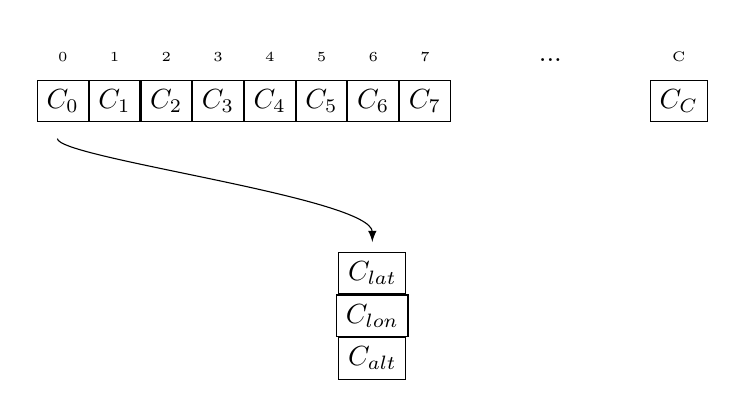
\begin{tikzpicture} [draw, minimum width=0.5cm, minimum height=0.5cm]
      \matrix(vector)[matrix of nodes,
          row 1/.style={nodes={draw=none, minimum width=0.3cm}},
          nodes={draw}] at (-1,2)
      {
          \tiny{0} & \tiny{1} & \tiny{2} & \tiny{3} & \tiny{4} & \tiny{5} & \tiny{6} & \tiny{7} & [1cm]... & [1cm]\tiny{C}\\
          $C_{0}$ & $C_{1}$ & $C_{2}$ & $C_{3}$ & $C_{4}$ & $C_{5}$ & $C_{6}$ & $C_{7}$ &  & $C_{C}$\\
      };
      
      \matrix (queue)[matrix of nodes, nodes={draw, nodes={draw, minimum height=0.6}}, nodes in empty cells] at (-1,-1)
    {
       $C_{lat}$\\ $C_{lon}$\\ $C_{alt}$\\
    };
    
    \draw[-latex] (-5,1.25) .. controls (-5,1) and (-1,0.5) .. (queue.north);
\end{tikzpicture}
\caption{Lista inicial de coordenadas}
\end{figure}

Este es uno de los primeros puntos donde se realiza un compromiso, ya que los dos puntos entre los que se calcula una distancia y pendiente corresponden a los diferentes puntos en una carretera o calle en los que se encuentran posibles desvíos (lo que en un mapa se corresponde a los nodos de unión). Este hecho puede derivar a que en zonas urbanas, la distancia que pueda existir entre los puntos que representan dos cruces consecutivos de calles sea bastante corta, por lo que la diferencia espacial entre ambos puntos es mínima y consecuentemente la pendiente también. Sin embargo, en autovías o autopistas puede haber distancias de varios kilómetros entre dichos puntos, con sus consiguientes curvas, en el plano horizontal, y con algunos tramos con mayor o menor inclinación que la media calculada posteriormente entre ambos puntos, tal y como puede verse en la figura \ref{fig:figSlopes}.

\begin{figure}[ht]
    \begin{subfigure}[b]{0.5\linewidth}
        \centering
        \includegraphics[width=0.75\linewidth]{City_Slope.png}
        \label{fig:figCitySlope}
        \caption{Puntos en entorno urbano}
    \end{subfigure}
    \begin{subfigure}[b]{0.5\linewidth}
        \centering
        \includegraphics[width=0.75\linewidth]{Highway_Slope.png} 
        \label{fig:figHighwaySlope}
        \caption{Puntos en autovía}
    \end{subfigure}
    \caption{Pendiente entre puntos}
    \label{fig:figSlopes}
\end{figure}

Para el procesado de estas rutas, la unidad de referencia que se ha creado es el \textit{chunk}. Cada uno de estos \textit{chunks} se corresponden al espacio correspondiente a dos coordenadas consecutivas ($C_{i}$ y $C_{i+1}$). A partir de dichas coordenadas, se obtiene para cada uno de estos \textit{chunks} la distancia entre sus dos coordenadas y la pendiente entre las mismas, teniendo ya en cuenta las restricciones mencionadas anteriormente. Para el cálculo de la distancia entre dos puntos, se utiliza la fórmula del semiverseno\footnote{\url{https://es.wikipedia.org/wiki/Fórmula\_del\_semiverseno} } (o más conocida como \textit{Haversine} en inglés) para calcular la distancia de círculo máximo entre las dos coordenadas. Y para la pendiente, se calcula la diferencia entre las alturas correspondientes a las coordenadas y se divide entre la distancia calculada previamente.

% Figura 2
\begin{wrapfigure}{r}{0.5\textwidth}
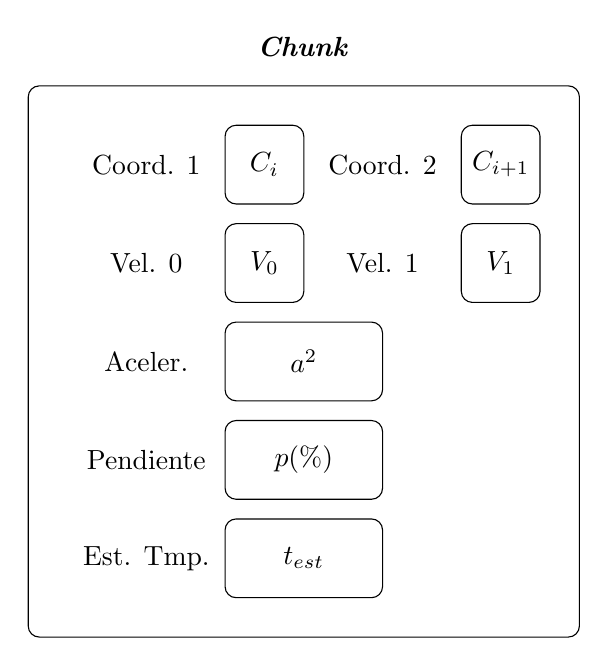
\begin{tikzpicture}[node distance=0cm]
    \node (C1) [nodointSq, draw=black] at (1.5,0) {$C_{i}$}; 
    \node (C1void) [] at (0,0) {Coord. 1};
    \node (C2) [nodointSq, draw=black] at (4.5,0) {$C_{i+1}$};
    \node (C2void) [] at (3,0) {Coord. 2};
    
    \node (V1) [nodointSq, draw=black] at (1.5,-1.25) {$V_{0}$}; 
    \node (V1void) [] at (0,-1.25) {Vel. 0};
    \node (V2) [nodointSq, draw=black] at (4.5,-1.25) {$V_{1}$};
    \node (V2void) [] at (3,-1.25) {Vel. 1};
    
    \node (AccVoid) [align=left] at (0,-2.5) {Aceler.};
    \node (Acc) [nodointRec, draw=black] at (2,-2.5) {$a^2$};
    
    \node (SlopeVoid) [align=left] at (0,-3.75) {Pendiente};
    \node (Slope) [nodointRec, draw=black] at (2,-3.75) {$p(\%)$};
    
    \node (EstVoid) [align=left] at (0,-5) {Est. Tmp.};
    \node (Est) [nodointRec, draw=black] at (2,-5) {$t_{est}$};
    
    \node (ALL) [minimum width=7cm, minimum height=7cm, rounded corners, draw=black] at (2,-2.5) {};
    \node (Title) [above of=ALL] at (2,1.5) {\textit{\textbf{Chunk}}};
\end{tikzpicture}
\caption{Representación de un \textit{chunk}}
\end{wrapfigure}

Además de las coordenadas, y la distancia y pendiente entre las mismas, dentro de cada \textit{chunk} se almacena otra información relativa a cada una de las iteraciones e individuos del algoritmo genético, que se corresponden a:
\begin{itemize}
    \item[$V_{0}$] Esta es la velocidad inicial del vehículo al pasar por la coordenada $C_{i}$ del \textit{chunk}. En el \textit{chunk} inicial, el valor es siempre 0, y para el resto de \textit{chunks}, este valor se asigna automáticamente al valor $V_{1}$ calculado del \textit{chunk} anterior.
    \item[$V_{1}$] Esta es la velocidad que tendrá el vehículo a pasar por la coordenada $C_{i+1}$ del \textit{chunk}. El cálculo de este valor se explica con detalle más adelante.
    \item[$t_{est}$] Tiempo estimado en recorrer la distancia del \textit{chunk} basado en la velocidad inicial $V_{0}$.
\end{itemize}{}

\textbf{Modelo de consumo}\newline
Como ya se ha mencionado anteriormente, este primer modelo se basa en una serie de aproximaciones, con bastantes libertades, al propio problema. Para realizar el cálculo del consumo de una ruta propuesta, se aprovecha el mismo proceso de creación de los \textit{chunks}. En este proceso, se pueden distinguir los siguientes pasos:

\begin{itemize}
    \item \textbf{Cálculo de la velocidad de crucero}. Este punto se centra en calcular cual es la aceleración estimada que tendría que hacer el vehículo para mantener la velocidad actual. Esta estimación, se realiza basándose en la velocidad de entrada al \textit{chunk}, $V_{0}$. Así pues, se definen 5 segmentos de velocidades, para los cuales, se establece cual debería de ser su aceleración para mantener la velocidad.
    \begin{table}[h]
    \centering
    \begin{tabular}{|l|l|l|l|}
    \hline
    \textbf{Segmento} & \textbf{Lim. Inferior} & \textbf{Lim. Superior} & \textbf{Acel. (0-1)} \\ \hline
    A        & 0             & 19            & 0.15         \\ \hline
    B        & 20            & 39            & 0.20         \\ \hline
    C        & 40            & 69            & 0.25         \\ \hline
    D        & 70            & 99            & 0.35         \\ \hline
    E        & 100           & 120           & 0.50         \\ \hline
    \end{tabular}
    \caption{Valores de interpolación para los segmentos de aceleración}
    \label{tab:v1_accel_interp}
    \end{table}
    
    A partir de estos niveles de aceleración, situada entre 0 y 1, se realiza una interpolación directa para situar dicho valor entre los niveles de consumo mínimo y máximo de un vehículo.
    
    \item \textbf{Cálculo de la velocidad de salida}. A partir de los datos de entrada relativos a la velocidad inicial en el tramo ($V_{0}$), la pendiente entre las coordenadas y la aceleración propuesta; y la aceleración asociada a la velocidad de crucero calculada en el paso anterior, ya se procede al cálculo de la velocidad de salida ($V_{1}$). Para ello, se utilizan de nuevo unos segmentos, para diferenciar en este caso por el nivel de pendiente. De esta forma, para que haya un aumento efectivo de la velocidad, la aceleración propuesta debe de ser superior a la estimada como de crucero y un factor asociado a la pendiente. En la tabla \ref{tab:v1_slope_accel}, se pueden ver los factores utilizados para dicho modelo.
    
    Estos factores se encuentran dentro del rango (0-1), siendo análogos a los rangos de aceleración. Así, por ejemplo, un factor de 0.1 sobre la aceleración en un tramo cuya $V_{0}$ se encuentre en el segmento B será equivalente a una aceleración de 0.3 sobre la posible aceleración de un vehículo.
    
    \begin{table}[h]
    \centering
    \begin{tabular}{|l|l|l|l|}
    \hline
    \textbf{Pendiente (\%)} & \textbf{Factor} \\ \hline
    0       &   0       \\ \hline
    +2      &   +0.1    \\ \hline
    +5      &   +0.2    \\ \hline
    +10     &   +0.25   \\ \hline
    -2      &   -0.1    \\ \hline
    -5      &   -0.2    \\ \hline
    -10     &   -0.25   \\ \hline
    \end{tabular}
    \caption{Valores de aceleración asociados a la pendiente}
    \label{tab:v1_slope_accel}
    \end{table}
\end{itemize}

\textbf{Preproceso de la iteración}\newline
Previamente a la ejecución en si de los bloques asociados a lo que sería el algoritmo genético como tal, se realiza el proceso previo encargado de obtener el consumo de cada uno de los individuos existentes en un momento dado, basándose en el modelo expuesto. De esta forma, ya se puede contar con la puntuación asociada a cada uno de los individuos, y así proceder hacia la siguiente generación.

Para el cálculo del consumo de cada uno de estos individuos, este se considera como la fuerza realizada, así, de cada uno de los \textit{chunks}, si su aceleración en ese periodo es superior a 0, se recalcula de nuevo la relación entre la aceleración realizada en el rango (0-1) y los consumos reales del vehículo, dividiendo el valor resultante entre los segundos estimados en los que el vehículo recorre el espacio asociado a un \textit{chunk}. Con los valores de consumo de cada \textit{chunk}, finalmente se realiza una suma de todos ellos obteniendo así el consumo asociado a un individuo.

Al final de este proceso, antes de entregar el valor asociado al consumo, se realiza una última comprobación para descartar, o más bien, detectar, posibles individuos inválidos. Esta comprobación se basa en la detección de que, en cualquier momento de la ruta, la velocidad calculada como $V_{1}$ en los diferentes \textit{chunks} que la conforman, no supera la velocidad máxima de la vía por la que discurre ese segmento. En tal caso, el individuo se indica como inválido devolviendo un consumo negativo (-1).\newline

\textbf{Iteración del algoritmo}\newline
En cuanto a las modificaciones relacionadas directamente con el uso de un algoritmo genético, estas son el cruce y la mutación. En este modelo, ambas opciones son bastante sencillas.

\begin{itemize}
    \item \textbf{Cruce}. En este caso el cruce se realiza por parejas de individuos contiguas (si el número de individuos es impar, el último individuo no se mezcla en esa iteración). Para realizar el cruce, se recorre a los dos individuos, y, por cada uno de los segmentos asociados a un \textit{chunk}, se calcula una probabilidad aleatoria. En el caso de superar un umbral previamente definido, se reemplazan los segmentos de ambos individuos entre sí.
\end{itemize}

% Figura 3
\begin{figure}[ht]
\centering
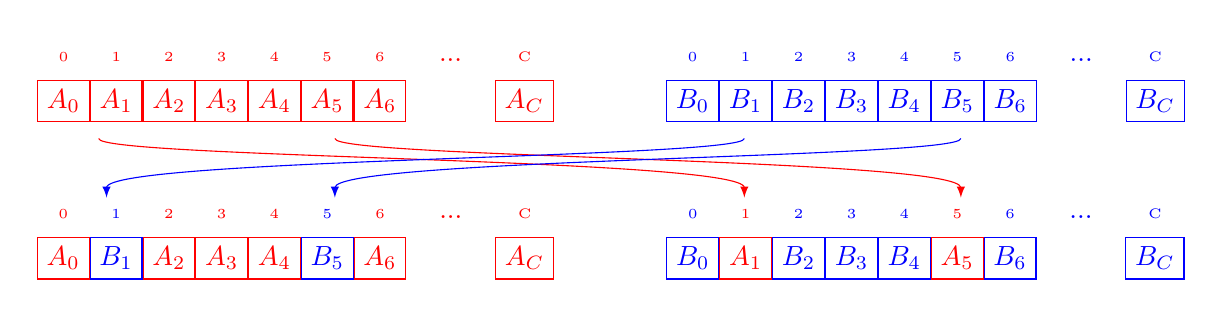
\begin{tikzpicture} [draw, minimum width=0.5cm, minimum height=0.5cm]
      \matrix(vector1)[matrix of nodes,
          row 1/.style={nodes={draw=none, minimum width=0.3cm}},
          nodes={draw}, red] at (-4,2)
      {
          \tiny{0} & \tiny{1} & \tiny{2} & \tiny{3} & \tiny{4} & \tiny{5} & \tiny{6} & [0.3cm]... & [0.3cm]\tiny{C}\\
          $A_{0}$ & $A_{1}$ & $A_{2}$ & $A_{3}$ & $A_{4}$ & $A_{5}$ & $A_{6}$ & & $A_{C}$\\
      };
      
      \matrix(vector2)[matrix of nodes,
          row 1/.style={nodes={draw=none, minimum width=0.3cm}},
          nodes={draw}, blue] at (4,2)
      {
          \tiny{0} & \tiny{1} & \tiny{2} & \tiny{3} & \tiny{4} & \tiny{5} & \tiny{6} & [0.3cm]... & [0.3cm]\tiny{C}\\
          $B_{0}$ & $B_{1}$ & $B_{2}$ & $B_{3}$ & $B_{4}$ & $B_{5}$ & $B_{6}$ & & $B_{C}$\\
      };
      
      \matrix(cvector1)[matrix of nodes,
          row 1/.style={nodes={draw=none, minimum width=0.3cm}},
          nodes={draw}, red] at (-4,0)
      {
          \tiny{0} & |[text=blue]| \tiny{1} & \tiny{2} & \tiny{3} & \tiny{4} & |[text=blue]| \tiny{5} & \tiny{6} & [0.3cm]... & [0.3cm]\tiny{C}\\
          $A_{0}$ & |[blue]|$B_{1}$ & $A_{2}$ & $A_{3}$ & $A_{4}$ & |[blue]|$B_{5}$ & $A_{6}$ & & $A_{C}$\\
      };
      
      \matrix(cvector2)[matrix of nodes,
          row 1/.style={nodes={draw=none, minimum width=0.3cm}},
          nodes={draw}, blue] at (4,0)
      {
          \tiny{0} & |[text=red]|\tiny{1} & \tiny{2} & \tiny{3} & \tiny{4} & |[text=red]|\tiny{5} & \tiny{6} & [0.3cm]... & [0.3cm]\tiny{C}\\
          $B_{0}$ & |[red]|$A_{1}$ & $B_{2}$ & $B_{3}$ & $B_{4}$ & |[red]|$A_{5}$ & $B_{6}$ & & $B_{C}$\\
      };
    
    \draw[-latex, red] (-6.5,1.25) .. controls (-6.5,1) and (1.7,1) .. (1.7,0.5);
    \draw[-latex, red] (-3.5,1.25) .. controls (-3.5,1) and (4.45,1) .. (4.45,0.5);
    
    \draw[-latex, blue] (1.7,1.25) .. controls (1.7,1) and (-6.4,1) .. (-6.4,0.5);
    \draw[-latex, blue] (4.45,1.25) .. controls (4.45,1) and (-3.5,1) .. (-3.5,0.5);
\end{tikzpicture}
\caption{Modelo básico: Diagrama de cruce entre individuos}
\end{figure}
\begin{itemize}
    \item \textbf{Mutación}. Para este caso, por cada uno de los individuos resultantes de la fase de cruce, se vuelve a calcular un valor aleatorio, y en el caso de superar un nuevo umbral, se decide aplicar una mutación a dicho individuo. En el caso afirmativo, por cada uno de los segmentos de los que se conforma el individuo, se aumenta o disminuye la aceleración aplicada en un 10\%, con una probabilidad idéntica para ambos casos. Adicionalmente, para no modificar a todos los segmentos de un individuo, se calcula un tercer valor aleatorio para decidir si se modifica dicho segmento. Es decir, se calcula un nuevo valor aleatorio para decidir si en la modificación se aumenta o disminuye la aceleración y adicionalmente un segundo valor para aplicar o no dicha modificación.
\end{itemize}
\newpage

\subsection{Modelo avanzado}
A partir del modelo anterior, en esta segunda iteración se propone el uso de un nuevo modelo de consumo ya preexistente, adaptado a las necesidades del problema abordado. Este se trata del VT-CPEM (\textit{Virginia Tech Comprehensive Power-based EV consumption Model}) \cite{FIORI2016257}. Este modelo es una evolución de un modelo de consumo, presentado por la misma entidad, pero relativo a los motores de combustión interna tradicionales, el VT-CPFM. Este modelo fue presentado en el año 2016, y cuenta en la actualidad con más de 260 referencias de otros artículos relacionados con el ámbito de los vehículos eléctricos, en su amplia mayoría de organizaciones externas a la de la publicación, como podría ser \cite{ZENG2019}, también con más de 230 citas o \cite{YUAN2017}, con más de 50 citas.

Ambos modelos están originalmente planteados dentro del ámbito de la predicción dentro de los ciclos de consumo, específicamente los ciclos relacionados con la EPA (\textit{U.S. Environmental Protection Agency}). Además de esta agencia, dada la similitud entre estos ciclos, los modelos desarrollados originalmente mantienen su validez en los ciclos relacionados con la NEDC (\textit{New European Driving Cycle}). En este punto, cabe remarcar, que tanto los ciclos de consumo de la EPA como del NEDC han sido reemplazados por los ciclos WLTP (\textit{World harmonized Light-duty vehicles Test Procedure}). Es por eso, que donde es posible, se utilizan los valores obtenidos en las pruebas realizadas en ciclos WLTP como entrada a estos modelos, y, por lo tanto, al modelo utilizado para este caso. Adicionalmente, el modelo VT-CPEM, al tratarse de una publicación más reciente ha sido creado teniendo en cuenta estos nuevos ciclos, para los que ofrece unos resultados incluso mejores si se compara con los ciclos anteriores como el NEDC \cite{FIORI2016257}.

A través del modelo VT-CPEM se realiza el cálculo de tres elementos diferentes:
\begin{itemize}
    \item \textbf{Consumo instantáneo}. Para el cálculo de este valor se tienen en cuenta una serie de valores, principalmente relacionados con la velocidad, la aceleración y una serie de características relacionadas con el entorno y el vehículo en sí. A partir de estos datos, se obtiene la energía consumida en una unidad de tiempo, que, en este caso, es cada segundo.
    
    Para calcular dicho valor, el modelo originalmente propone el uso de la siguiente fórmula:
    \begin{align*}
        P_{Wheels}(t) = & \left(ma(t) + mg\cdot cos(\vartheta) \cdot \frac{C_{r}}{1000}(C_{1}v(t) + c_{2}) + \right. \\ 
        & \left. \frac{1}{2}\rho_{Air}A_{f}C_{D}v^{2}(t) + mg \cdot sin(\vartheta) \right) \cdot v(t)
    \end{align*}
    Donde los valores utilizados se corresponden a la siguiente distribución:
    \begin{itemize}
        \item $m$ - Masa del vehículo (en $kg$).
        \item $v(t)$ - Velocidad del vehículo en el instante a calcular (en $m/s$).
        \item $a(t)$ - Aceleración del vehículo en el instante a calcular (en $m/s^2$).
        \item $\vartheta$ - Inclinación de la calzada (introducida como $rad$).
        \item $C_{r}, C_{1}, C{2}$ - Coeficientes de rozamiento del vehículo con la superficie (1.75, 0.0328 y 4.575 respectivamente) \cite{RAKHA2001}.
        \item $\rho_{Air}$ - Densidad del aire en una superficie a nivel del mar y a una temperatura media ($1.2256$ en $kg/m^3$).
        \item $A_{f}$ - Área frontal del vehículo (en $m^2$).
        \item $C_{d}$ - Coeficiente de rozamiento del vehículo con el aire.
        \item $g$ - Constante de aceleración gravitatoria en la tierra ($9.8066$ $m/s^2$).
    \end{itemize}
    
    Al utilizar dicha fórmula, se realiza una especie de sumatorio entre todas las fuerzas que intervienen en el movimiento del vehículo, principalmente, la fuerza ejercida por el motor, contrarrestada por los rozamientos aerodinámicos y de rozamiento y la pendiente.
    
    Dado que este cálculo se debe de realizar por cada tramo que conforma una ruta, por cada uno de los individuos que conforman la población del algoritmo genético y en cada una de las iteraciones a procesar, para evitar una sobrecarga de operaciones que a la larga conllevan un tiempo de cómputo superior, se han simplificado algunos de los parámetros que son constantes durante toda la ejecución, quedando de la siguiente forma:
    
    \begin{align*}
        P_{Wheels}(t) = & \left(ma(t) + A \cdot cos(\vartheta) \cdot (C_{1}v(t) + c_{2}) + B \cdot v^{2}(t) + C \cdot sin(\vartheta) \right) \cdot v(t)
    \end{align*}
    
    Donde $A$ sería la constante obtenida de $mg \cdot \frac{C_{r}}{1000}$ y $B$ la constante obtenida de $\frac{1}{2}\rho_{Air}A_{f}C_{D}$ y $C$ simplemente el cálculo de $mg$.
    
    % Figura 4
    \begin{figure}[ht]
    \centering
    \begin{tikzpicture}
        \node [rotate=12] (car) at (0,0) {\includegraphics[width=0.25\textwidth]{dummy_car.png}};
        
        \draw[-latex] (1.5,0) .. controls (3,0) and (3.5,0) .. (5,0) node[midway, above]{$ma(t)$};
        \draw[-latex] (-1.5,0) .. controls (-4,0) and (-4.5,0) .. (-6,0)  node[midway, above]{$\frac{1}{2}\rho_{Air}A_{f}C_{D}v^{2}(t)$};
        \draw[-latex] (0,0) .. controls (0,-1) and (0,-1.5) .. (0,-2) node[midway, right]{$mg\cdot cos(\vartheta) \cdot \frac{C_{r}}{1000}(C_{1}v(t) + c_{2})$};
        \draw[-latex] (0,0) .. controls (0,0) and (-2.2,-0.5) .. (-5,-1) node[left, above]{$mg \cdot sin(\vartheta)$};
    \end{tikzpicture}
    \caption{Modelo avanzado: distribución de fuerzas que interactúan}
    \end{figure}
    
    Esta fuerza resultante se corresponde a la fuerza ejercida por las ruedas del vehículo para alcanzar la velocidad y aceleración indicadas como valores de entrada. Es por ello, que para calcular el consumo real producido por el motor (o motores) eléctricos que conforman el vehículo hay que tener en consideración una serie de factores que incrementan el valor de $P_{Wheels}(t)$.
    \begin{itemize}
        \item Eficiencia de la transmisión $\eta_{Driveline}$. El valor utilizado para dicho factor es 0.92 \cite{RAKHA2011492}.
        \item Eficiencia del motor eléctrico $\eta_{Electric Motor}$. Este valor puede fluctuar entre el rango de 0.85 a 0.95, dependiendo del vehículo y sus características.
    \end{itemize}
    
    Teniendo en cuenta estos factores, se puede obtener la energía consumida realmente en un instante de tiempo dado, es decir, los kW que se consumen como entrada en un motor para generar movimiento.
    \begin{align*}
        P_{EM}(t) = P_{Wheels}(t) \cdot \eta_{Driveline}^{-1} \cdot \eta_{Electric Motor}^{-1}
    \end{align*}
    
    En el caso en el que $P_{EM}(t)$ sea menor que 0, se considera que el vehículo estará frenando. En dicho caso, un nuevo factor entra en escena, tratándose en este caso, del factor de eficiencia de frenada regenerativa $\eta_{RB}$, es decir, la energía que el vehículo es capaz de absorber del proceso de frenada.
    
    Al contrario que los factores mencionados anteriormente, este factor es dependiente de la aceleración del vehículo en dicho instante. Si la aceleración aplicada es positiva, el valor es 0, en el caso contrario (la frenada es efectiva), el valor se calcula de la siguiente forma:
    
    \begin{align*}
        \eta_{RB}(t) = \left[ \exp \left( \frac{0.0411}{a(t)} \right) \right] ^{-1}
    \end{align*}
    
    \item \textbf{Estado de la carga}.
    A partir del consumo instantáneo calculado anteriormente para un instante de tiempo dado, es posible saber cuál será el estado de carga de la batería de un vehículo en un instante dado. Para ello, por cada uno de los instantes donde se calcula un consumo, se calcula a cuanto porcentaje de la batería se corresponde para ir retirándolo del total disponible. 
    
    Para realizar este cálculo es necesario tener en cuenta el factor de eficiencia de la batería, $\eta_{Battery}$, que se corresponde a las perdidas producidas en la distribución de la energía desde la batería hasta los motores, el cual se establece como 0.9 \cite{RYDH20051957}. Adicionalmente, también hay que tener en cuenta los posibles equipos auxiliares del vehículo, como podría ser el sistema multimedia o de climatización. Este consumo está considerado de media como de 700W.
    
    \begin{align*}
        SC_{Final}(t) &= SC_{0} - \sum_{i=1}^{N}{\Delta SC_{i}(t)} \\
        \Delta SC_{i}(t) &= SC_{i-1}(t) - \frac{P_{EM}(t) \cdot \eta_{Battery}^{-1} + P_{Aux}}{3600 \cdot Capacity_{Batt}}
    \end{align*}
    
    \item \textbf{Energía total consumida}. Con los datos obtenidos y las fórmulas ya descritas, es posible obtener finalmente el consumo total de un vehículo para una ruta dada. Para ello, se integra relativo al tiempo el consumo del vehículo teniendo en cuenta como punto inicial el instante $t=0$ y como final, el instante el punto $t=T$, siendo T el tiempo transcurrido en realizar la ruta.
    
    \begin{align*}
        EC = \frac{1}{3600} \cdot \int_{0}^{T}{P_{EM}(t)dt} \quad(kWh)
    \end{align*}
    
    Para facilitar la realización de estos cálculos, se ha reutilizado la estructura basada en \textit{chunks} del modelo anterior. De esta forma, la energía consumida, se calcula independientemente en cada uno de los \textit{chunks} sumando al final el coste de todos ellos. Este modelo permite introducir una simplificación que se trata de que, por cada uno de los \textit{chunks}, la aceleración es constante en el mismo. Para los \textit{chunks} pequeños esto no supone ningún problema; y, en el caso de aquellos más largos (varios kilómetros), en el caso óptimo la aceleración utilizada debería de tender a 0 o a un valor ligeramente superior que mantuviese la velocidad constante. Con esto, el cálculo de la energía consumida, se puede simplificar a:
    
    \begin{align*}
        EC = \frac{1}{3600} \cdot \sum_{C_i=0}^{N} \lim_{\Delta x\to0} \sum_{t=0}^{T_{est}}{P_{EM}(t)\Delta t} \quad(kWh)
    \end{align*}
    
    Con esta pequeña restricción, se facilita el cálculo de la velocidad de salida del \textit{chunk} y el tiempo estimado en recorrer el mismo. Es por eso, que a partir de las ecuaciones de movimiento (uniformemente acelerado), es posible obtener dichos valores, a través de las siguientes ecuaciones:
    
    \begin{align*}
        V_{1} &= \sqrt{V_{0}^{2} + 2 a_{c} \Delta s} \\
        T_{est} &= abs \left( \frac{V_{1} - V_{0}}{a_{c}} \right)
    \end{align*}
\end{itemize}

\subsubsection{Algoritmo genético}
\label{section:adv_gen_alg}
\noindent\textbf{Preprocesado de la ruta}\newline
\label{Adv_AG}
Con este nuevo modelo, se ha añadido un nuevo elemento de configuración al sistema de predicción, llamado el \textit{margen entre puntos}. La finalidad de este nuevo valor consiste en agilizar y simplificar los cálculos a realizar durante las iteraciones del algoritmo genético. Este valor se elige entre los diferentes elementos disponibles en un desplegable a través de la interfaz gráfica, y antes de la carga de los datos de la ruta a realizar. Todos estos valores se corresponden a una distancia en metros.

Así, cuando se obtiene la información de la ruta, se comprueba punto a punto si la distancia entre el punto a procesar y el último añadido a la ruta es superior al \textit{margen} establecido. Gracias este preprocesado de los puntos, se logra eliminar aquellos puntos que se encuentren muy cerca entre ellos, y que, a la larga, durante la ejecución del algoritmo, implican un tiempo de cálculo para cada uno de los individuos en cada iteración.

Los valores disponibles para elegir son: 5, 10, 15, 20, 50 y 100 metros. Esta variedad da la posibilidad de elegir el margen de forma que este se encuentre en un compromiso entre la longitud de la ruta y la precisión de los puntos. Es decir, en rutas muy cortas se elegiría un valor pequeño, de forma que la simulación permita acercarse más a un valor real, mientras que, para rutas muy largas, lo más adecuado sea utilizar un valor alto, de forma que no se consuma una gran cantidad de potencia de cálculo en zonas con puntos muy cercanos que en el conjunto final de la ruta no aportan una diferencia.\newline

\begin{figure}[!htb]
    \centering
    \includegraphics[width=0.75\textwidth]{Margin_map_2r.png}
    \caption{Puntos de una ruta}
    \label{fig:margin_points}
\end{figure}

Este hecho permitiría, en el caso de la figura \ref{fig:margin_points}, simplificar los puntos de las dos rotondas por donde transcurre esta ruta de prueba, sobre todo, el conjunto de puntos entre el 10 y el 15, los cuales se encuentran muy juntos entre sí, y que, a efectos de la conducción de un vehículo, se pueden considerar prácticamente idénticos entre ellos.

\noindent\textbf{Generación de individuos}\newline
De forma similar al modelo básico, al inicio de la ejecución, una vez ya obtenidos los datos necesarios tanto de la ruta a procesar como el vehículo a utilizar, se procede a generar un grupo inicial de individuos.

De forma paralela, aprovechando todos los hilos de ejecución disponibles en un dispositivo, se van creando individuos de forma aleatoria. Por cada uno de estos individuos, se calcula su puntuación, para posteriormente determinar si es un individuo válido, en cuyo caso se añade al grupo con el que se iniciará la iteración del algoritmo.

Uno de los puntos a tener en cuenta cuando se realiza un trayecto en un vehículo (ya sea eléctrico o no) es el confort del mismo durante la conducción. Uno de los puntos que influyen en este confort se trata de la realización de una conducción suave, que evite tanto acelerones fuertes como frenadas bruscas. Este hecho influye, además, de la misma forma, en el consumo de un vehículo, ya que tanto una aceleración fuerte como la recuperación tras una frenada son uno de los puntos donde más consumo se realiza (bien de combustible o de batería). Es por ello, que, en la población inicial, los valores aleatorios se distribuyen entre -0.5 y 0.5, siendo el rango total entre -1 y 1, simulando así unos supuestos casos de conducción más suaves con los que iniciar el problema. Dichos rangos se pueden definir de la siguiente forma para los instantes 0 y q:
\begin{align*}
    X_{i,j}^{0} \in [-0.5, 0.5] \\
    X_{i,j}^{q} \in [-1, 1]
\end{align*}

\noindent\textbf{Iteración del algoritmo}\newline
Para realizar las diferentes iteraciones del algoritmo el paso esencial es el cálculo de las puntuaciones asociadas a cada individuo. Para esto, se utilizan las técnicas ya mencionadas anteriormente basadas en el modelo VT-CPEM. Una vez obtenida esta puntuación, se pasa a los siguientes pasos:

\begin{itemize}
    \item \textbf{Cruce}. El primer paso previo a realizar el cruce de los individuos se trata de realizar una clasificación de los mismos, en este caso basada en NGR (\textit{Normalised Geometric Ranking} o Clasificación Geométrica Normalizada). Dicha normalización se basa en una serie de valores, $q$ y $q_0$. Basándose en \cite{GARZELLI2008223}, el valor de $q$ se define como 0.1, siendo el que mejores resultados ofrece en el uso de esta clasificación. A partir de dicho valor, se calcula $q_0$ de la siguiente forma, siendo P el número de individuos:
    \begin{align*}
        q_{0} = q / (1 - (1 - q)^{P})
    \end{align*}
    A continuación, partiendo de los individuos ordenados por su puntuación obtenida, se pasa a obtener la probabilidad de ser escogidos, de la siguiente forma, y siendo $r$ la posición de un individuo ordenado por la puntuación de los mismos.
    \begin{align*}
        P_{i} = q_{0} \cdot (1 - q)^{r_{i}-1} 
    \end{align*}
    
    Una vez obtenida esta probabilidad para individuo, se eligen como candidatos para el cruce a aquellos cuyo valor se sitúe por encima de $0.4 \cdot q$ o bien hasta alcanzar el límite de candidatos para el cruce; situado en el 40\% de la población.
    
    Una vez elegidos los individuos a cruzar, estos pasan a cruzarse en pares siguiendo un cruce aritmético. Los elementos que conforman un par para realizar el cruce no se encuentran ordenados, de forma que se evita que, pese a ser los mejores de toda la población, los dos primeros únicamente se crucen entre ellos y así sucesivamente. Para realizar el cruce, se elige un número aleatorio, $r$ de una distribución uniforme entre 0 y 1, y se aplica la siguiente solución, siendo $\Vec{X}$ y $\Vec{Y}$ los individuos originales y $\Vec{X}'$ y $\Vec{Y}'$ los nuevos.
    \begin{align*}
        \Vec{X}' = r\Vec{X} + (1-r)\Vec{Y} \\
        \Vec{Y}' = (1-r)\Vec{X} + r\Vec{Y}
    \end{align*}
    
    Finalmente, estos nuevos individuos creados pasan a reemplazar a aquellos que obtuvieron peor resultado durante la última iteración del algoritmo.
    
    % Figura 5
    \begin{figure}[ht]
    \centering
    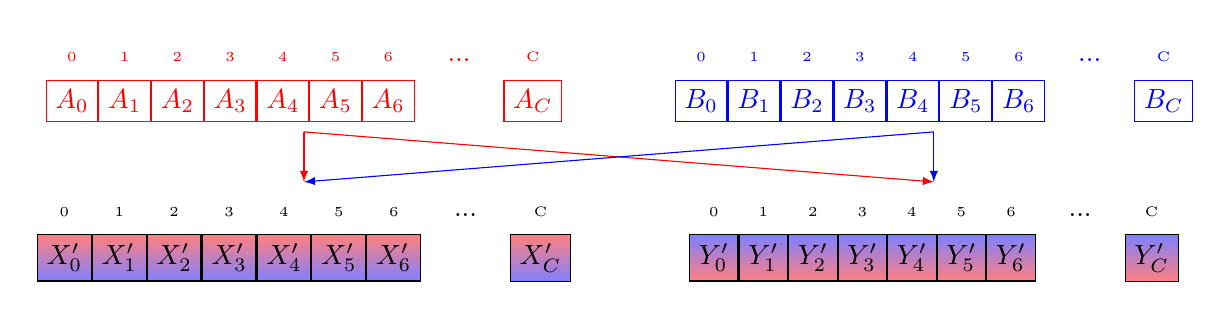
\begin{tikzpicture} [draw, minimum width=0.5cm, minimum height=0.5cm]
      \matrix(vector1)[matrix of nodes,
          row 1/.style={nodes={draw=none, minimum width=0.3cm}},
          nodes={draw}, red] at (-4,2)
      {
          \tiny{0} & \tiny{1} & \tiny{2} & \tiny{3} & \tiny{4} & \tiny{5} & \tiny{6} & [0.3cm]... & [0.3cm]\tiny{C}\\
          $A_{0}$ & $A_{1}$ & $A_{2}$ & $A_{3}$ & $A_{4}$ & $A_{5}$ & $A_{6}$ & & $A_{C}$\\
      };
      
      \matrix(vector2)[matrix of nodes,
          row 1/.style={nodes={draw=none, minimum width=0.3cm}},
          nodes={draw}, blue] at (4,2)
      {
          \tiny{0} & \tiny{1} & \tiny{2} & \tiny{3} & \tiny{4} & \tiny{5} & \tiny{6} & [0.3cm]... & [0.3cm]\tiny{C}\\
          $B_{0}$ & $B_{1}$ & $B_{2}$ & $B_{3}$ & $B_{4}$ & $B_{5}$ & $B_{6}$ & & $B_{C}$\\
      };
      
      \matrix(cvector1)[matrix of nodes,
          row 1/.style={nodes={draw=none, minimum width=0.3cm}},
          nodes={draw}] at (-4,0)
      {
          \tiny{0} & \tiny{1} & \tiny{2} & \tiny{3} & \tiny{4} & \tiny{5} & \tiny{6} & [0.3cm]... & [0.3cm]\tiny{C}\\
          |[top color=red!50, bottom color=blue!50]| $X_{0}'$ & |[top color=red!50, bottom color=blue!50]|$X_{1}'$ & |[top color=red!50, bottom color=blue!50]|$X_{2}'$ & |[top color=red!50, bottom color=blue!50]|$X_{3}'$ & |[top color=red!50, bottom color=blue!50]|$X_{4}'$ & |[top color=red!50, bottom color=blue!50]|$X_{5}'$ & |[top color=red!50, bottom color=blue!50]|$X_{6}'$ & & |[top color=red!50, bottom color=blue!50]|$X_{C}'$\\
      };
      
      \matrix(cvector2)[matrix of nodes,
          row 1/.style={nodes={draw=none, minimum width=0.3cm}},
          nodes={draw}] at (4,0)
      {
          \tiny{0} & \tiny{1} & \tiny{2} & \tiny{3} & \tiny{4} & \tiny{5} & \tiny{6} & [0.3cm]... & [0.3cm]\tiny{C}\\
          |[top color=blue!50, bottom color=red!50]|$Y_{0}'$ & |[top color=blue!50, bottom color=red!50]|$Y_{1}'$ & |[top color=blue!50, bottom color=red!50]|$Y_{2}'$ & |[top color=blue!50, bottom color=red!50]|$Y_{3}'$ & |[top color=blue!50, bottom color=red!50]|$Y_{4}'$ & |[top color=blue!50, bottom color=red!50]|$Y_{5}'$ & |[top color=blue!50, bottom color=red!50]|$Y_{6}'$ & & |[top color=blue!50, bottom color=red!50]|$Y_{C}'$\\
      };
    
    \draw[-latex, red] (vector1.south) -- (cvector1.north);
    \draw[-latex, red] (vector1.south) -- (cvector2.north);
    
    \draw[-latex, blue] (vector2.south) -- (cvector1.north);
    \draw[-latex, blue] (vector2.south) -- (cvector2.north);
\end{tikzpicture}
\caption{Modelo avanzado: Diagrama de cruce entre individuos}
\end{figure}

    \item \textbf{Mutación}. La mutación en este caso es bastante sencilla, y similar a la aplicada en el modelo básico. Del grupo de población resultante de la fase de cruce, para cada uno de los individuos, se calcula una probabilidad uniforme, y en el caso de ser superior a un umbral ($x>0.9, x \in [0,1]$ por defecto), se pasa a aplicar una mutación sobre el individuo.
    
    La mutación que se le aplica a un individuo consiste en reemplazar un elemento de entre los que conforman la lista de aceleraciones. De esta forma, la modificación realizada no es tan pronunciada, tal y como ocurría en el modelo anterior, lo que permite que el individuo resultante tenga más posibilidades de ser válido. Para el elemento a reemplazar, el nuevo valor, estará comprendido entre 0 y 1, obteniéndose a partir de una distribución uniforme.
    
    \item \textbf{Reinicio}. Una vez realizadas las modificaciones tanto de cruce como de mutación y se calculan las puntuaciones de los individuos, se realiza una última comprobación con el objetivo de intentar detectar si la simulación realizada se ha quedado estancada en un mínimo local. Para ello, si durante un número dado de iteraciones consecutivas no se consigue mejorar la mejor puntuación obtenida, se hace un reinicio de la población.
    
    Para definir cuantas iteraciones son consideradas como determinantes en este cálculo, se ha definido como elemento clave el 15\% del número total de iteraciones definidas para un cálculo, permitiendo así, en el peor de los casos (o el de mayor número de reinicios) un total de 6 reinicios durante una ejecución.
    
    En cuanto al procedimiento de reinicio, este es bastante sencillo. Dada una población, se guarda únicamente al mejor individuo registrado hasta dicho momento y se procede a regenerar el resto de la población de nuevo. Dado que este mejor individuo utilizado se guarda, en el caso en el que, tras un reinicio, este individuo se pueda ver cruzado o mutado y no mejore su puntuación obtenida, en el siguiente proceso de reinicio vuelve a ser rescatado para ser incluido en la nueva población de nuevo en su estado original de cuando obtuvo la mejor puntuación.
\end{itemize}

\noindent\textbf{Limitaciones aplicadas}\newline
Además de las propias limitaciones a tener en cuenta basadas en el entorno automovilístico en el que se desarrolla el proyecto, y que ya se ha mencionado anteriormente, como son los límites de velocidad de las diferentes vías por las que transcurre una ruta a analizar, también se ha añadido una segunda restricción a los individuos generados para poder considerarlos válidos tras una iteración.

Esta restricción se trata de forzar que, para un instante de tiempo $t$, que vendría a ser representado por un \textit{chunk} que conforma un individuo, su velocidad de salida, $v1$, debe de ser por lo menos igual o superior a la mitad de la velocidad establecida como límite en la vía que se está utilizando en dicho instante.

Esta restricción se hace necesaria ya que, en algunos casos, especialmente cuando la métrica de optimización se centra en mejorar únicamente el consumo eléctrico del vehículo, al no añadir la limitación, el resultado obtenido, aun siendo el mejor en cuanto a consumo, no es factible a ser realizado por un vehículo real en un entorno real, dado que su realización supondría ser un peligro durante la conducción.

\subsubsection{Métricas alternativas}
\label{section:adv_alt_models}
Partiendo de la base desarrollada con el modelo avanzado, se han realizado dos aproximaciones adicionales relativas a lo que vendría a ser la función de coste del algoritmo genético. Estas aproximaciones se basan en modificar el objetivo a minimizar durante la ejecución del algoritmo. Así, si inicialmente el elemento a buscar se trata de aquel que consiga realizar una ruta dada con el menor consumo posible, se añaden las posibilidades de priorizar que se realice dicha ruta en el menor tiempo posible y una tercera opción, que combina las dos anteriores.\newline

\noindent\textbf{Métricas basadas en el tiempo}\newline
En esta aproximación, el procedimiento a la hora de obtener los datos, procesarlos al inicio, la creación de los individuos y el funcionamiento general del algoritmo genético es prácticamente similar. La principal diferencia es la simplificación de los cálculos que se realizan por cada uno de los \textit{chunks} de un individuo para calcular su puntuación, ya que no se hace necesario realizar el cálculo del consumo eléctrico, manteniendo únicamente el cálculo de la velocidad de salida, $v_{1}$, y del tiempo estimado, $T_{est}$. Es este segundo valor del tiempo estimado en recorrer un \textit{chunk}, el que se acaba sumando por cada uno de los \textit{chunks} que componen un individuo para obtener su puntuación.

Una vez obtenida esta puntuación, el procedimiento ya existente para obtener los mejores individuos en una iteración y realizar las operaciones de cruce y mutación establecidas, junto a las diferentes correcciones necesarias. El método para elegir a dicho mejor individuo se mantiene igual que con la métrica original, dado que al igual que ocurre con los consumos, a menor tiempo, un individuo es considerado como mejor.\newline

\noindent\textbf{Métricas mixtas}\newline
Esta última aproximación se centra en la combinación de las dos anteriores, o, dada la simplicidad del uso de la métrica basada únicamente en el tiempo, más bien añadir dicha funcionalidad a todo el conjunto ya desarrollado basado en el consumo eléctrico del vehículo.

Como ocurre con las dos aproximaciones anteriores, el procesado de un individuo se realiza analizando los \textit{chunks} de los que se compone. Para este caso, por cada uno de los \textit{chunks}, en lugar de extraer un único valor asociado a la puntuación, se extraen tanto el consumo realizado en dicho \textit{chunk}, $P_{EM}$, como el tiempo estimado en recorrerlo, $T_{est}$. Dado que estos dos valores obtenidos se tratan de elementos completamente diferentes (consumo en W/h y tiempo en segundos), se hace necesario realizar una normalización previa a las diferentes comparaciones entre individuos.

Esta normalización se basa en obtener el valor máximo de cada una de las puntuaciones (es decir, el del peor elemento), y aplicar una interpolación entre la puntuación obtenida en cada uno de los factores y su máximo a una escala entre 0 y 10. Para mantener también la compatibilidad con el resto de funcionalidad previamente desarrollada en la aproximación inicial, aquellos individuos que no son válidos se dejan con valor -1 para su posterior identificación y corrección.

Una vez ambas medidas ya son comparables, el paso final antes de proseguir con la identificación del mejor individuo consiste en realizar una combinación de las dos puntuaciones. Tal y como se expresa con la fórmula que se encuentra a continuación, al hacer una ponderación entre ambas puntuaciones, es posible definir dinámicamente, para diferentes ejecuciones del algoritmo, si se le quiere seguir dando más prioridad a alguna de las dos variantes (valor de $r$ distinto a 0.5), o, si, por el contrario, basta con realizar una media de los dos valores obtenidos ($r$ igual a 0.5).

\begin{align*}
    \Vec{Sc} = r \cdot \Vec{ConsWh} + (1-r) \cdot \Vec{ConsS} \\
\end{align*}
    
Con esto, se obtiene la lista $Sc$, con las puntuaciones ponderadas de todos los individuos en una iteración, a partir de la cual ya se puede realizar una ordenación y aplicar las diferentes técnicas relativas al propio algoritmo genético descritas anteriormente. Dado que la puntuación se calcula cada iteración, este nuevo cálculo se tendrá que realizar en cada una de estas, añadiendo por tanto un tiempo adicional al cómputo total de tiempo de procesamiento de la solución.

\newpage
\section{Extracción de resultados}
\label{results_visualization}
Una vez finalizada la ejecución del algoritmo, se hace necesario representar de una forma concreta y clara la mejor solución obtenida tras la ejecución. Para ello, se propone una representación, similar a la de los ejemplos mostrados en el capítulo \ref{AnalisisProblema} y que se puede observar en la figura \ref{fig:result_demo}.

% Figura 6
\begin{figure}[!htb]
\centering
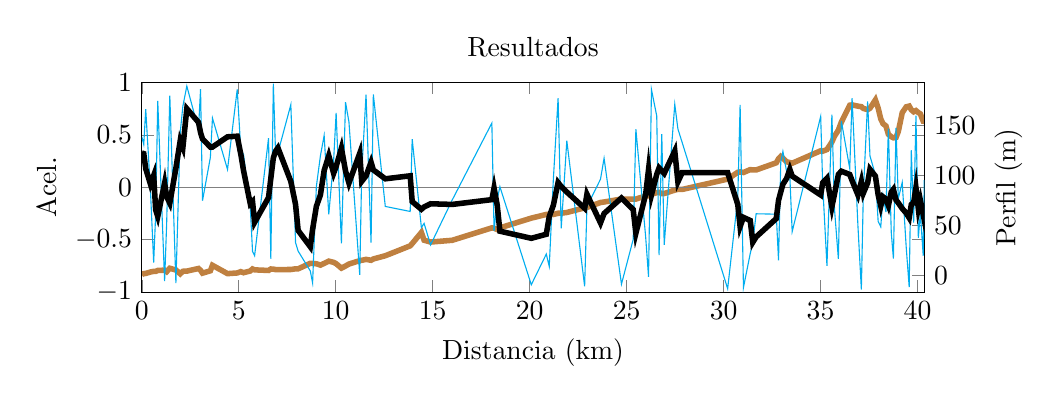
\begin{tikzpicture}
\pgfplotsset{%
    width=0.95\textwidth,
    height=0.35\textwidth
}
 \begin{axis}[
      axis y line*=right,
      axis x line=none,
      ylabel=Perfil (m),
      xmin=0,xmax=40346
    ]
    \addplot[color=brown, line width=2pt] coordinates {(0,0.87)(102.164,1.96)(203.92700000000002,2.08)(447.94500000000005,3.55)(613.325,4.17)(716.186,4.11)(823.47,5.07)(1176.592,5.38)(1282.9530000000002,3.84)(1445.4260000000002,7.25)(1759.0880000000002,5.55)(1982.15,1.73)(2119.9010000000003,4.26)(2322.943,4.41)(2924.277,7.04)(3030.437,5.18)(3130.813,2.38)(3536.143,4.74)(3644.949,10.22)(4420.9130000000005,1.9)(4921.3240000000005,2.56)(5104.733,3.87)(5245.344,2.82)(5594.861,4.54)(5710.807,6.57)(5817.772,5.68)(6534.901,5.07)(6654.088,6.53)(6783.7,6.45)(6902.016,5.91)(7020.003,5.97)(7685.297,6.03)(7928.504,6.71)(8062.249,6.71)(8688.872,12.23)(8807.58,12.11)(9002.436,11.74)(9210.017,10.43)(9403.583,12.11)(9641.305,14.38)(9892.713,13.19)(10020.635,11.84)(10293.636,7.4)(10506.469000000001,9.53)(10681.998000000001,11.49)(11237.900000000001,14.9)(11340.149000000001,15.22)(11563.322000000002,16.15)(11821.782000000003,15.26)(11939.827000000003,16.58)(12555.680000000002,19.79)(13839.171000000002,29.7)(13943.060000000001,31.97)(14416.667000000001,43.08)(14556.487000000001,35.35)(14890.702000000001,33.49)(16008.686000000002,35.26)(18050.462000000003,47.68)(18164.586000000003,47.34)(18325.663000000004,46.02)(18465.065000000002,47.71)(20084.003000000004,57.43)(20857.488000000005,61.1)(21009.720000000005,61.43)(21221.142000000003,61.07)(21465.656000000003,62.3)(21627.590000000004,62.37)(21915.516000000003,63.08)(22834.536000000004,67.72)(22952.991000000005,68.13)(23651.793000000005,73.07)(23836.670000000006,73.57)(24733.588000000007,76.53)(25338.191000000006,76.46)(25476.630000000005,76.46)(25981.370000000006,79.68)(26128.677000000007,79.76)(26280.104000000007,81.27)(26551.986000000008,82.92)(26672.823000000008,83.2)(26812.049000000006,82.04)(26937.280000000006,82.06)(27482.118000000006,85.47)(27643.210000000006,86.22)(27865.914000000008,86.13)(30208.929000000007,96.47)(30729.789000000008,103.29)(30851.175000000007,103.63)(31022.892000000007,103.08)(31373.032000000007,105.97)(31504.037000000008,105.6)(31676.333000000006,105.6)(32714.764000000006,112.78)(32831.530000000006,116.81)(32947.049000000006,119.15)(33057.22000000001,117.42)(33247.047000000006,113.82)(33414.321,113.0)(33535.26500000001,112.36)(35005.57600000001,124.81)(35109.21000000001,124.4)(35328.725000000006,126.05)(35584.062000000005,133.63)(35718.11400000001,139.43)(35917.28500000001,145.46)(36070.40500000001,153.45)(36503.86500000001,170.4)(36623.96900000001,170.76)(36926.16700000001,169.43)(37102.41000000001,168.93)(37205.05900000001,167.17)(37425.69800000001,165.97)(37546.65000000001,167.33)(37826.07800000001,175.65)(37968.48600000001,167.58)(38103.27700000001,156.65)(38220.99300000001,151.89)(38369.83800000001,149.67)(38495.22200000001,141.33)(38645.14800000001,138.8)(38754.81700000001,137.76)(38890.53500000001,138.18)(39007.28600000001,144.07)(39209.689000000006,162.84)(39413.97000000001,168.76)(39568.76400000001,169.54)(39678.03100000001,165.82)(39799.18100000001,163.8)(39916.84600000001,165.02)(40040.41400000001,163.02)(40144.534000000014,161.74)(40292.13800000001,154.38)(40345.99300000002,154.23)};
    \end{axis}
  \begin{axis}[
      title={Resultados},
      xlabel={Distancia (km)},
      ylabel={Acel.},
      ymin=-1,ymax=1,xmin=0,xmax=40346,
      scaled x ticks = false,
      xtick={0,5000,10000,15000,20000,25000,30000,35000,40000},
      xticklabels={0,5,10,15,20,25,30,35,40}]
      
      \addplot[color=gray] coordinates {(0,0)(40346,0)};
      
      \addplot[color=cyan] coordinates {(0,0.48303786)(102.164,0.4087189)(203.92700000000002,0.74541871)(447.94500000000005,-0.03099373)(613.325,-0.71799794)(716.186,-0.25708803)(823.47,0.82503353)(1176.592,-0.89579131)(1282.9530000000002,-0.34495415)(1445.4260000000002,0.8750705)(1759.0880000000002,-0.91393511)(1982.15,0.52156396)(2119.9010000000003,0.7759734)(2322.943,0.96535861)(2924.277,0.55244227)(3030.437,0.93556825)(3130.813,-0.12765526)(3536.143,0.28469026)(3644.949,0.66023547)(4420.9130000000005,0.1703067)(4921.3240000000005,0.93424731)(5104.733,0.35968597)(5245.344,0.31310484)(5594.861,-0.19239181)(5710.807,-0.61165505)(5817.772,-0.65262612)(6534.901,0.46799668)(6654.088,-0.68217857)(6783.7,0.98927139)(6902.016,0.30171766)(7020.003,0.32994364)(7685.297,0.78817003)(7928.504,-0.52764639)(8062.249,-0.60871957)(8688.872,-0.79791019)(8807.58,-0.91208745)(9002.436,0.00949483)(9210.017,0.29965309)(9403.583,0.49499163)(9641.305,-0.25738089)(9892.713,0.25853082)(10020.635,0.70977536)(10293.636,-0.53438638)(10506.469000000001,0.81140644)(10681.998000000001,0.62299643)(11237.900000000001,-0.83478558)(11340.149000000001,0.13924977)(11563.322000000002,0.88416122)(11821.782000000003,-0.52723948)(11939.827000000003,0.88548626)(12555.680000000002,-0.18235783)(13839.171000000002,-0.23037173)(13943.060000000001,0.45994851)(14416.667000000001,-0.38382441)(14556.487000000001,-0.34455891)(14890.702000000001,-0.54900648)(16008.686000000002,-0.1203613)(18050.462000000003,0.612956)(18164.586000000003,-0.41536831)(18325.663000000004,-0.1160324)(18465.065000000002,0.00579139)(20084.003000000004,-0.92957245)(20857.488000000005,-0.63705045)(21009.720000000005,-0.7551067)(21221.142000000003,0.07651198)(21465.656000000003,0.85066378)(21627.590000000004,-0.39170798)(21915.516000000003,0.44444547)(22834.536000000004,-0.9446756)(22952.991000000005,-0.18433026)(23651.793000000005,0.07708568)(23836.670000000006,0.27749306)(24733.588000000007,-0.92375565)(25338.191000000006,-0.49682093)(25476.630000000005,0.55522302)(25981.370000000006,-0.47370418)(26128.677000000007,-0.85345045)(26280.104000000007,0.93255504)(26551.986000000008,0.68141618)(26672.823000000008,-0.64725583)(26812.049000000006,0.50641209)(26937.280000000006,-0.54817083)(27482.118000000006,0.79232902)(27643.210000000006,0.55701787)(27865.914000000008,0.42626929)(30208.929000000007,-0.96735136)(30729.789000000008,-0.10498194)(30851.175000000007,0.78627818)(31022.892000000007,-0.956224)(31373.032000000007,-0.63227536)(31504.037000000008,-0.52795437)(31676.333000000006,-0.25251361)(32714.764000000006,-0.25616557)(32831.530000000006,-0.69695879)(32947.049000000006,0.24040537)(33057.22000000001,0.34257397)(33247.047000000006,0.15128995)(33414.321,0.10870376)(33535.26500000001,-0.42212792)(35005.57600000001,0.67604427)(35109.21000000001,0.02135457)(35328.725000000006,-0.74896034)(35584.062000000005,0.69268448)(35718.11400000001,-0.20984079)(35917.28500000001,-0.68353137)(36070.40500000001,0.63252321)(36503.86500000001,0.17895029)(36623.96900000001,0.85133016)(36926.16700000001,-0.36836149)(37102.41000000001,-0.9747614)(37205.05900000001,-0.05169141)(37425.69800000001,0.81879303)(37546.65000000001,0.29956233)(37826.07800000001,0.11954253)(37968.48600000001,-0.32615156)(38103.27700000001,-0.37677139)(38220.99300000001,-0.07464349)(38369.83800000001,-0.23595292)(38495.22200000001,0.55861449)(38645.14800000001,-0.43290058)(38754.81700000001,-0.6807297)(38890.53500000001,0.56767519)(39007.28600000001,-0.10721657)(39209.689000000006,0.04713388)(39413.97000000001,-0.56852504)(39568.76400000001,-0.95231977)(39678.03100000001,0.35347062)(39799.18100000001,-0.33703526)(39916.84600000001,0.68380121)(40040.41400000001,-0.48117133)(40144.534000000014,-0.24069175)(40292.13800000001,-0.65261272)(40345.99300000002,0.06811072)};

        \addplot[color=black, line width=2pt] coordinates {(0,0.3274351)(102.164,0.32123635)(203.92700000000002,0.17763676)(447.94500000000005,0.02961158)(613.325,0.11287451)(716.186,-0.2153675)(823.47,-0.27815958)(1176.592,0.04045411)(1282.9530000000002,-0.09091531)(1445.4260000000002,-0.15160922)(1759.0880000000002,0.18274372)(1982.15,0.44480627)(2119.9010000000003,0.38028063)(2322.943,0.7501813)(2924.277,0.62033745)(3030.437,0.52208083)(3130.813,0.4610562)(3536.143,0.38462908)(3644.949,0.3843649)(4420.9130000000005,0.48183314)(4921.3240000000005,0.48751606)(5104.733,0.3169906)(5245.344,0.16059825)(5594.861,-0.15677643)(5710.807,-0.13511429)(5817.772,-0.33417098)(6534.901,-0.09783834)(6654.088,0.08483621)(6783.7,0.28135016)(6902.016,0.34538483)(7020.003,0.37629126)(7685.297,0.05669307)(7928.504,-0.1632325)(8062.249,-0.41163872)(8688.872,-0.56737376)(8807.58,-0.40191386)(9002.436,-0.18117162)(9210.017,-0.07306576)(9403.583,0.1610579)(9641.305,0.301114)(9892.713,0.13430611)(10020.635,0.19758907)(10293.636,0.37366453)(10506.469000000001,0.15500125)(10681.998000000001,0.04089614)(11237.900000000001,0.32460566)(11340.149000000001,0.05687647)(11563.322000000002,0.10937444)(11821.782000000003,0.23985999)(11939.827000000003,0.16593569)(12555.680000000002,0.08109315)(13839.171000000002,0.10977616)(13943.060000000001,-0.13623287)(14416.667000000001,-0.2095626)(14556.487000000001,-0.18756052)(14890.702000000001,-0.15695902)(16008.686000000002,-0.1632678)(18050.462000000003,-0.1175625)(18164.586000000003,-0.00660292)(18325.663000000004,-0.16844515)(18465.065000000002,-0.41844644)(20084.003000000004,-0.48639412)(20857.488000000005,-0.44788525)(21009.720000000005,-0.27891077)(21221.142000000003,-0.17133788)(21465.656000000003,0.04496131)(21627.590000000004,0.00704753)(21915.516000000003,-0.04512092)(22834.536000000004,-0.19983654)(22952.991000000005,-0.06599633)(23651.793000000005,-0.33963655)(23836.670000000006,-0.25006562)(24733.588000000007,-0.10215496)(25338.191000000006,-0.21231293)(25476.630000000005,-0.43850164)(25981.370000000006,-0.0672395)(26128.677000000007,0.16840792)(26280.104000000007,-0.07208785)(26551.986000000008,0.12393541)(26672.823000000008,0.18499133)(26812.049000000006,0.15694613)(26937.280000000006,0.13206646)(27482.118000000006,0.34677149)(27643.210000000006,0.0520188)(27865.914000000008,0.14065658)(30208.929000000007,0.13944641)(30729.789000000008,-0.16320197)(30851.175000000007,-0.3749109)(31022.892000000007,-0.2870315)(31373.032000000007,-0.31653783)(31504.037000000008,-0.52502658)(31676.333000000006,-0.47317354)(32714.764000000006,-0.2986374)(32831.530000000006,-0.12453173)(32947.049000000006,-0.04377102)(33057.22000000001,0.02920285)(33247.047000000006,0.08416903)(33414.321,0.17129681)(33535.26500000001,0.10705293)(35005.57600000001,-0.07299713)(35109.21000000001,0.04379901)(35328.725000000006,0.08625644)(35584.062000000005,-0.18565869)(35718.11400000001,-0.06342496)(35917.28500000001,0.12215716)(36070.40500000001,0.1538863)(36503.86500000001,0.12218216)(36623.96900000001,0.06393615)(36926.16700000001,-0.07290677)(37102.41000000001,0.05506178)(37205.05900000001,-0.05529179)(37425.69800000001,0.04228902)(37546.65000000001,0.17201098)(37826.07800000001,0.10699499)(37968.48600000001,-0.07169232)(38103.27700000001,-0.17879537)(38220.99300000001,-0.09098097)(38369.83800000001,-0.11233078)(38495.22200000001,-0.17312244)(38645.14800000001,-0.0446587)(38754.81700000001,-0.01891144)(38890.53500000001,-0.12120756)(39007.28600000001,-0.14833245)(39209.689000000006,-0.20265046)(39413.97000000001,-0.24549138)(39568.76400000001,-0.29145511)(39678.03100000001,-0.16412165)(39799.18100000001,-0.14665091)(39916.84600000001,-0.0043253)(40040.41400000001,-0.20554197)(40144.534000000014,-0.12451277)(40292.13800000001,-0.26127302)(40345.99300000002,-0.16503875)};
      \end{axis}
   
\end{tikzpicture}
\caption{Ejemplo de posible resultado}
\label{fig:result_demo}
\end{figure}

En esta figura, aparecen dos series de datos extraídas a partir de la misma solución alcanzada tras la ejecución del algoritmo genético. Ambas soluciones comparten tanto el eje X horizontal como el eje Y vertical izquierdo. Dicho eje X se corresponde a la distancia (en kilómetros) recorrida desde el inicio de la ruta hasta la llegada al destino. En cuanto al eje Y izquierdo, este corresponde a una representación de la aceleración aplicada en el transcurso de cada uno de los \textit{chunks} que conforman la mejor solución. Dicha aceleración se encuentra escalada a un rango entre -1 y 1, siendo -1 la aplicación de la máxima frenada posible en el vehículo y 1 la máxima aceleración posible, respectivamente.

En cuanto a las series de datos, la primera de ellas, representada en azul, se corresponde al resultado directo obtenido de representar los valores del individuo marcado como el mejor tras la ejecución del algoritmo genético. Como se puede ver en el ejemplo, es bastante factible el caso en el que entre varios \textit{chunks} sucesivos, la aceleración establecida a aplicar sea dispar entre dichos puntos, generando picos bastante marcados.

Para suavizar estas representaciones dispares (y en muchos casos, irrealizables por un vehículo real), se utiliza la segunda serie de datos, de color negro, y un poco más marcada que la inicial, la cual representa los mismos datos que la serie inicial, pero aplicando una media móvil. De esta forma, se consigue suavizar la solución presentada de tal forma que la transición entre un punto y el siguiente en el transcurso de una ruta es más factible, realista y aplicable por un vehículo, sin perder a su vez la validez otorgada por el algoritmo genético tras su ejecución.

Finalmente, para otorgarle una representación a la solución aplicable al entorno real, se añade una tercera serie, marcada como una línea de color marrón, que se corresponde con el perfil de altitud de la ruta a realizar. Es por ello, que el eje X se corresponde idénticamente al de la solución propuesta, mientras que el eje Y, representado en la parte derecha, se corresponde con la altitud sobre el nivel del mar (en metros) de cada uno de los puntos que conforman la ruta.

\chapter{Pruebas}
\section{Modelo básico}
Una vez definido este primer modelo e implementado siguiendo la estructura indicada anteriormente. Se han ido realizando una serie de diferentes pruebas para determinar la calidad y el funcionamiento del mismo.

Para este primer modelo básico, debido a los datos que se muestran a continuación, se ha optado únicamente por realizar estas pruebas con un solo vehículo y con unos únicos puntos de origen y destino. El perfil de altura asociado a la ruta existente entre esos dos puntos es el mostrado en la figura \ref{fig:test_profile}.

\begin{figure}[ht]
    \centering
    \includegraphics[width=0.75\textwidth]{Demo_route_profile.png}
    \caption{Perfil de la ruta inicial de pruebas}
    \label{fig:test_profile}
\end{figure}

Con esta ruta definida, se han realizado una serie de 5 ejecuciones por cada una de las combinaciones a probar. Respecto al número de iteraciones del algoritmo, este se ha probado con 50, 100 y 200. Además, por cada una de estas cantidades de iteraciones, se ha realizado una prueba tanto con 30, como con 100 individuos.

Tal y como se puede ver en las gráficas presentadas en las figuras \ref{fig:basic_simulation_res_30} y \ref{fig:basic_simulation_res_100}, correspondientes a la puntuación obtenida por la función de \textit{fitness} del algoritmo genético, utilizando dicho modelo básico, la capacidad de aprendizaje es prácticamente nula, apareciendo únicamente algunos casos en los que se consigue mejorar la mejor puntuación en alguna de las series del caso.

Cada uno de los puntos que aparecen en estas gráficas se corresponden a la mejor puntuación obtenida por un individuo en una iteración dada del algoritmo. En el caso en el que durante una iteración no exista ningún individuo válido (ninguno cumple con las condiciones para que la ruta a realizar sea factible en términos de límites de velocidad), no se queda representado, apareciendo así algunos ``huecos`` entre las diferentes marcas.

Un hecho que puede observarse en todas las gráficas se corresponde a la relación según la cual, conforme se avanza en el número de iteraciones, la posibilidad de encontrar un individuo válido entre toda la población va disminuyendo, quedando pronunciadamente visible en los casos donde la población en menor (gráficas de la figura \ref{fig:basic_simulation_res_30}), donde aproximadamente a partir de la iteración 50, la dispersión de los puntos se vuelve muy notable, lo que equivale a una muy baja concentración de individuos válidos.

\begin{figure}[!htb]
% Figura 7
\begin{subfigure}[b]{0.43\textwidth}
\centering
\resizebox{\linewidth}{!}{
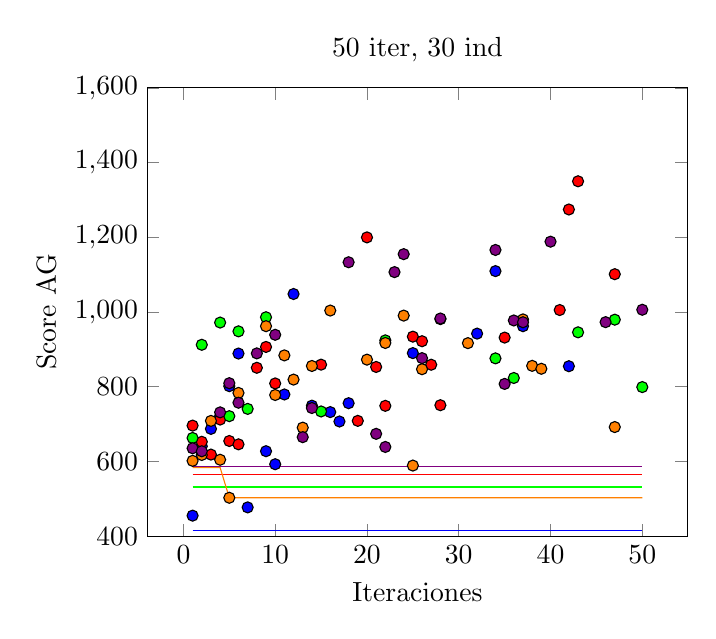
\begin{tikzpicture}
      \begin{axis}[
      title={50 iter, 30 ind},
      xlabel={Iteraciones},
      ylabel={Score AG},
      ymin=400,ymax=1600,
      ytick={400,600,...,1600}]
      
      \addplot[color=blue] coordinates {(1,414.688)(50,414.688)};
      \addplot[only marks, mark options={fill=blue}] coordinates {
      (1,455.002)(2,640.699)(3,687.203)(4,721.264)(5,801.565)(6,888.891)(7,477.115)(9,627.518)(10,592.660)(11,779.358)(12,1048.29)(14,749.370)(16,732.143)(17,706.989)(18,756.030)(25,890.072)(32,942.239)(34,1109.53)(37,962.117)(42,854.966)};
      
      \addplot[color=red] coordinates {(1,564.094)(50,564.094)};
      \addplot[only marks, mark options={fill=red}] coordinates {(1,696.036)(2,652.671)(3,618.431)(4,712.218)(5,654.812)(6,645.880)(8,850.792)(9,906.581)(10,808.870)(15,859.200)(19,708.717)(20,1199.78)(21,853.006)(22,748.915)(25,934.148)(26,921.873)(27,858.945)(28,750.592)(35,931.600)(41,1005.35)(42,1274.45)(43,1349.94)(47,1101.31)};
      
      \addplot[color=green] coordinates {(1,531.733)(50,531.733)};
      \addplot[only marks, mark options={fill=green}] coordinates {(1,662.945)(2,912.366)(4,971.847)(5,721.291)(6,948.300)(7,740.758)(9,986.071)(15,733.8689)(22,924.1769)(34,875.9981)(36,823.4571)(43,945.6761)(47,979.5601)(50,799.0926)};
      
      \addplot[color=orange] coordinates{(1,583.627)(4,583.627)(5,502.891)(50,502.891)};
      \addplot[only marks, mark options={fill=orange}] coordinates {(1,601.724)(2,617.433)(3,708.614)(4,604.592)(5,502.891)(6,783.532)(9,962.155)(10,777.942)(11,883.963)(12,819.152)(13,690.567)(14,855.631)(16,1003.95)(20,872.569)(22,917.214)(24,990.437)(25,589.059)(26,846.983)(28,980.998)(31,916.752)(37,980.284)(38,855.965)(39,848.146)(47,692.104)};
      
      \addplot[color=violet] coordinates {(1,586.663)(50,586.663)};
      \addplot[only marks, mark options={fill=violet}] coordinates {(1,635.361)(2,627.293)(4,731.443)(5,809.528)(6,757.276)(8,889.334)(10,939.062)(13,665.087)(14,743.085)(18,1133.24)(21,673.964)(22,638.867)(23,1106.84)(24,1154.95)(26,876.599)(28,982.704)(34,1166.16)(35,807.608)(36,977.438)(37,972.692)(40,1188.31)(46,972.919)(50,1006.10)};
      
      \end{axis}
\end{tikzpicture}}
\end{subfigure}
% Figura 8
\begin{subfigure}[b]{0.43\textwidth}
\centering
\resizebox{\linewidth}{!}{
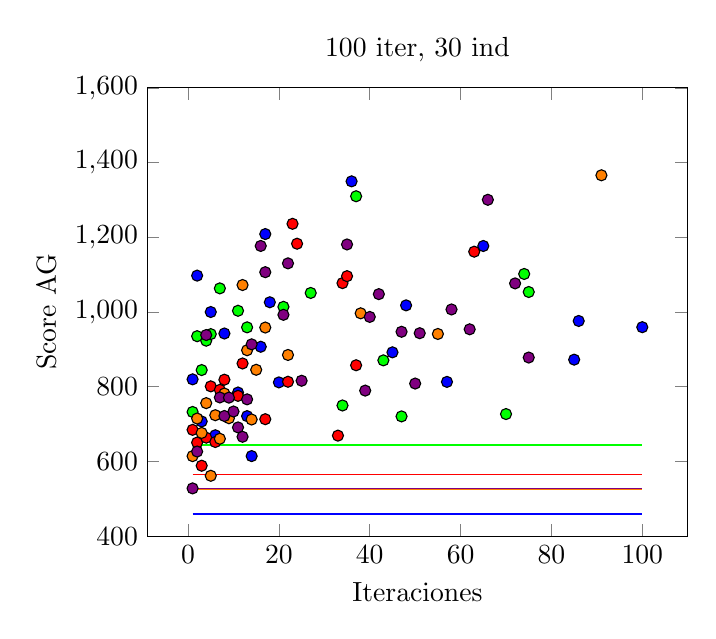
\begin{tikzpicture}
      \begin{axis}[
      title={100 iter, 30 ind},
      xlabel={Iteraciones},
      ylabel={Score AG},
      ymin=400,ymax=1600,
      ytick={400,600,...,1600}]
      
      \addplot[color=blue] coordinates {(1,459.431)(100,459.431)};
      \addplot[only marks, mark options={fill=blue}] coordinates {(1,819.856)(2,1097.47)(3,707.164)(5,1000.03)(6,670.172)(8,942.556)(11,784.586)(13,721.381)(14,614.402)(16,907.065)(17,1208.70)(18,1026.16)(20,811.678)(36,1349.81)(45,892.152)(48,1017.85)(57,813.033)(65,1176.81)(85,872.553)(86,976.110)(100,959.420)};
      
      \addplot[color=red] coordinates {(1,564.190)(100,564.190)};
      \addplot[only marks, mark options={fill=red}] coordinates {(1,684.672)(2,650.628)(3,588.617)(4,663.737)(5,801.069)(6,652.121)(7,791.738)(8,818.897)(11,775.640)(12,862.341)(17,713.155)(22,813.356)(23,1236.15)(24,1182.90)(33,669.169)(34,1077.40)(35,1096.02)(37,857.513)(63,1161.54)};
      
      \addplot[color=green] coordinates {(1,644.058)(100,644.058)};
      \addplot[only marks, mark options={fill=green}] coordinates {(1,732.523)(2,935.310)(3,844.689)(4,923.305)(5,940.877)(7,1063.31)(11,1003.38)(13,958.991)(21,1013.92)(27,1051.07)(34,749.904)(37,1309.90)(43,870.651)(47,720.655)(70,726.936)(74,1101.91)(75,1053.61)};
      
      \addplot[color=orange] coordinates {(1,524.214)(100,524.214)};
      \addplot[only marks, mark options={fill=orange}] coordinates {(1,614.304)(2,714.961)(3,676.362)(4,756.159)(5,561.712)(6,723.854)(7,660.789)(8,781.842)(9,715.805)(12,1072.32)(13,897.772)(14,712.343)(15,845.397)(17,958.507)(22,885.098)(38,996.581)(55,941.299)(91,1366.03)};
      
      \addplot[color=violet] coordinates {(1,527.978)(100,527.978)};
      \addplot[only marks, mark options={fill=violet}] coordinates {(1,527.978)(2,626.632)(4,938.403)(7,771.353)(8,721.746)(9,770.902)(10,733.737)(11,691.144)(12,666.081)(13,766.274)(14,913.553)(16,1176.89)(17,1106.66)(21,992.571)(22,1130.29)(25,816.087)(35,1180.89)(39,789.713)(40,986.924)(42,1047.93)(47,947.149)(50,808.579)(51,943.338)(58,1006.94)(62,953.785)(66,1300.42)(72,1076.66)(75,878.198)};

      \end{axis}
\end{tikzpicture}}
\end{subfigure}
\newline
\centering
% Figura 9
\begin{subfigure}[b]{0.43\textwidth}
\resizebox{\linewidth}{!}{
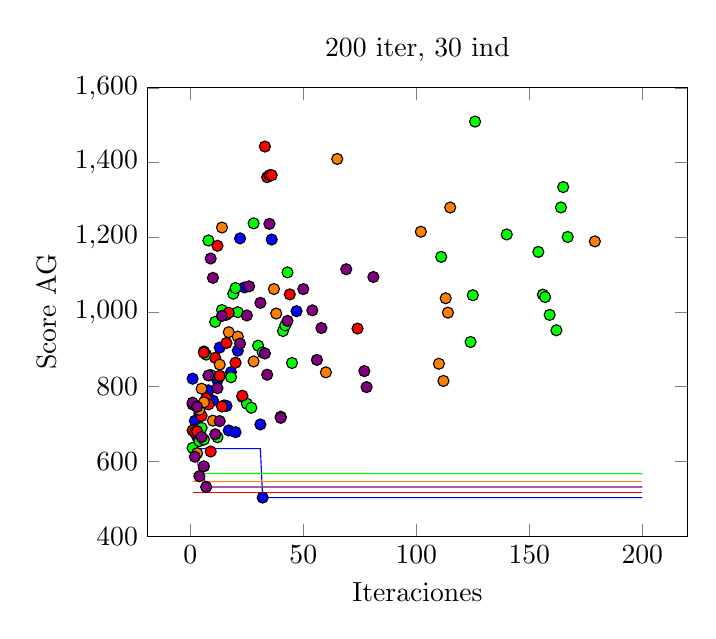
\begin{tikzpicture}
      \begin{axis}[
      title={200 iter, 30 ind},
      xlabel={Iteraciones},
      ylabel={Score AG},
      ymin=400,ymax=1600,
      ytick={400,600,...,1600}]
      
      \addplot[color=blue] coordinates {(1,634.298)(31,634.298)(32,503.287)(200,503.287)};
      \addplot[only marks, mark options={fill=blue}] coordinates {(1,821.595)(2,708.816)(3,667.164)(4,728.786)(6,894.330)(8,790.416)(10,762.906)(12,817.397)(13,905.012)(15,750.002)(16,748.767)(17,682.939)(18,838.977)(20,678.407)(21,896.569)(22,1197.18)(24,1065.87)(31,699.133)(32,503.287)(36,1194.07)(47,1002.28)};
      
      \addplot[color=green] coordinates {(1,567.917)(200,567.283)};
      \addplot[only marks, mark options={fill=green}] coordinates {(1,636.312)(2,685.176)(4,654.333)(5,689.890)(6,658.623)(7,886.028)(8,1191.53)(9,831.256)(11,973.696)(12,664.846)(13,828.474)(14,1005.33)(16,992.804)(18,825.471)(19,1049.02)(20,1064.21)(21,999.525)(23,772.981)(25,754.647)(27,743.817)(28,1237.35)(30,910.030)(32,891.872)(40,719.673)(41,949.235)(42,964.290)(43,1106.08)(45,863.617)(111,1147.68)(124,919.832)(125,1045.04)(126,1509.80)(140,1207.68)(154,1160.92)(156,1046.53)(157,1040.09)(159,992.426)(162,951.198)(164,1280.00)(165,1334.52)(167,1200.91)};
      
      \addplot[color=red] coordinates {(1,517.691)(200,517.691)};
      \addplot[only marks, mark options={fill=red}] coordinates {(1,683.021)(2,678.018)(3,680.827)(5,722.013)(6,891.317)(7,769.235)(8,752.731)(9,626.653)(11,877.428)(12,1177.33)(13,829.277)(14,747.185)(16,917.194)(17,998.077)(20,864.361)(23,776.012)(33,1442.96)(34,1360.87)(35,1366.21)(36,1366.21)(44,1047.25)(74,955.671)};
      
      \addplot[color=orange] coordinates {(1,547.137)(200,547.137)};
      \addplot[only marks, mark options={fill=orange}] coordinates {(1,752.877)(2,750.398)(3,621.830)(4,738.502)(5,794.827)(6,758.235)(10,709.293)(13,859.340)(14,1226.15)(17,946.074)(21,934.211)(28,867.729)(37,1061.58)(38,996.045)(60,838.628)(65,1409.77)(102,1214.91)(110,861.584)(112,815.561)(113,1036.86)(114,998.420)(115,1279.81)(179,1189.11)};
      
      \addplot[color=violet] coordinates {(1,639.028)(2,612.746)(3,612.746)(4,560.627)(6,560.627)(7,531.795)(200,531.795)};
      \addplot[only marks, mark options={fill=violet}] coordinates {(1,757.375)(2,612.7463)(3,746.4429)(4,560.6270)(5,665.4716)(6,587.0324)(7,531.795)(8,830.145)(9,1143.28)(10,1091.44)(11,672.840)(12,796.148)(13,708.127)(14,989.638)(22,915.605)(25,990.804)(26,1068.78)(31,1024.57)(33,889.160)(34,832.229)(35,1236.03)(40,716.617)(43,976.403)(50,1061.38)(54,1004.49)(56,871.854)(58,957.142)(69,1114.57)(77,841.834)(78,799.051)(81,1093.72)};
      
      \end{axis}
\end{tikzpicture}}
\end{subfigure}
\caption{Ejecuciones del modelo básico (30 ind.)}
\label{fig:basic_simulation_res_30}
\end{figure}


Al cambiar el número de individuos de 30 a 100, puede observarse como la densidad de los puntos en las gráficas aumenta, incrementando el umbral virtual mencionado ya anteriormente, donde se empieza a notar una gran dispersión en los puntos hasta aproximadamente las 100 iteraciones. Sin embargo, pese a una ligera mejora de los datos, se sigue sin conseguir en ningún momento que la tendencia general sea descendente, o, al menos sea más plana, por lo que queda de manifiesto la poca capacidad de aprendizaje de la que dispone el sistema al utilizar este modelo.

\begin{figure}[!htb]
% Figura 10
\begin{subfigure}[b]{0.43\textwidth}
\centering
\resizebox{\linewidth}{!}{
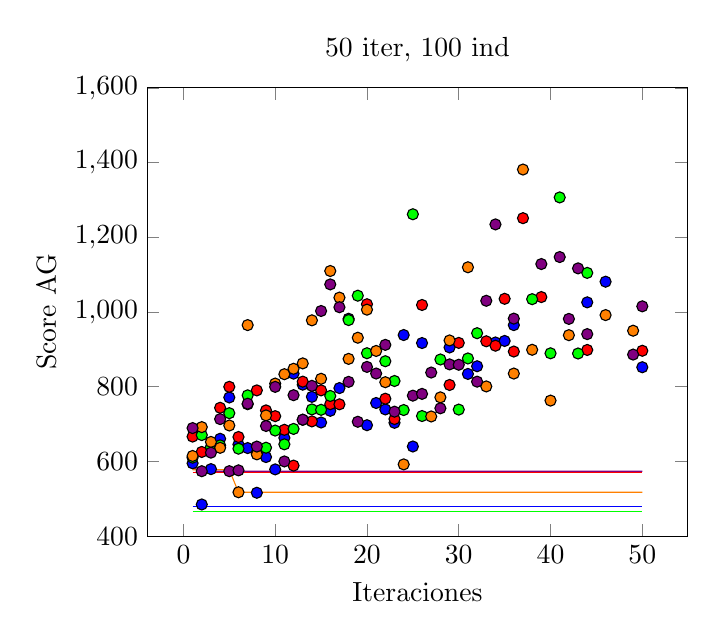
\begin{tikzpicture}
      \begin{axis}[
      title={50 iter, 100 ind},
      xlabel={Iteraciones},
      ylabel={Score AG},
      ymin=400,ymax=1600,
      ytick={400,600,...,1600}]
      
      \addplot[color=blue] coordinates {(1,480.411)(50,480.411)};
      \addplot[only marks, mark options={fill=blue}] coordinates {(1,595.160)(2,484.937)(3,579.550)(4,660.704)(5,771.356)(6,645.537)(7,635.908)(8,516.241)(9,611.817)(10,578.819)(11,663.110)(12,835.131)(13,805.609)(14,772.994)(15,704.318)(16,735.569)(17,796.436)(18,982.019)(20,697.095)(21,756.539)(22,739.343)(23,703.505)(24,938.456)(25,640.114)(26,916.993)(29,905.212)(31,834.323)(32,854.905)(34,918.540)(35,922.595)(36,965.075)(44,1025.92)(46,1081.22)(50,852.236)};
      
      \addplot[color=red] coordinates {(1,570.761)(50,570.761)};
      \addplot[only marks, mark options={fill=red}] coordinates {(1,666.642)(2,625.518)(3,637.730)(4,743.718)(5,799.822)(6,665.547)(7,753.268)(8,790.265)(9,736.724)(10,721.297)(11,684.754)(12,588.909)(13,813.687)(14,707.274)(15,790.326)(16,753.406)(17,752.983)(20,1020.88)(22,767.999)(23,713.646)(26,1018.88)(29,804.779)(30,917.405)(33,921.701)(34,909.883)(35,1035.41)(36,894.256)(37,1251.23)(39,1040.05)(44,898.484)(50,896.347)};
      
      \addplot[color=green] coordinates {(1,465.551)(50,465.551)};
      \addplot[only marks, mark options={fill=green}] coordinates {(1,610.178)(2,670.676)(3,638.131)(4,643.043)(5,729.275)(6,634.241)(7,776.965)(8,621.250)(9,636.824)(10,682.769)(11,645.883)(12,687.159)(13,711.591)(14,739.353)(15,738.276)(16,775.377)(18,978.533)(19,1043.74)(20,889.762)(22,868.319)(23,815.424)(24,737.664)(25,1261.74)(26,721.617)(28,873.006)(30,738.866)(31,875.751)(32,943.353)(38,1034.45)(40,889.532)(41,1306.76)(43,889.032)(44,1104.80)};
      
      \addplot[color=orange] coordinates{(1,577.728)(5,577.728)(6,517.625)(50,517.625)};
      \addplot[only marks, mark options={fill=orange}] coordinates {(1,614.761)(2,691.958)(3,652.320)(4,636.546)(5,696.337)(6,517.625)(7,965.025)(8,619.044)(9,723.293)(10,808.500)(11,833.631)(12,848.121)(13,862.561)(14,977.761)(15,821.315)(16,1109.85)(17,1038.63)(18,874.623)(19,931.215)(20,1006.35)(21,895.853)(22,812.202)(24,592.187)(27,720.461)(28,771.641)(29,923.968)(31,1119.81)(33,800.874)(36,835.343)(37,1381.42)(38,898.947)(40,762.916)(42,938.077)(46,991.824)(49,950.021)};
      
      \addplot[color=violet] coordinates {(1,584.276)(2,573.971)(50,573.971)};
      \addplot[only marks, mark options={fill=violet}] coordinates {(1,689.372)(2,573.971)(3,623.656)(4,713.423)(5,574.054)(6,576.227)(7,754.781)(8,639.887)(9,695.003)(10,799.688)(11,600.105)(12,777.430)(13,711.870)(14,802.439)(15,1002.80)(16,1074.00)(17,1012.84)(18,813.103)(19,706.279)(20,853.113)(21,835.444)(22,912.144)(23,733.319)(25,776.213)(26,780.920)(27,838.055)(28,742.329)(29,859.886)(30,858.915)(32,813.671)(33,1030.12)(34,1234.56)(36,982.372)(39,1128.47)(41,1147.16)(42,981.609)(43,1116.87)(44,940.924)(49,886.136)(50,1015.28)};
      
      \end{axis}
\end{tikzpicture}}
\end{subfigure}
% Figura 11
\begin{subfigure}[b]{0.43\textwidth}
\centering
\resizebox{\linewidth}{!}{
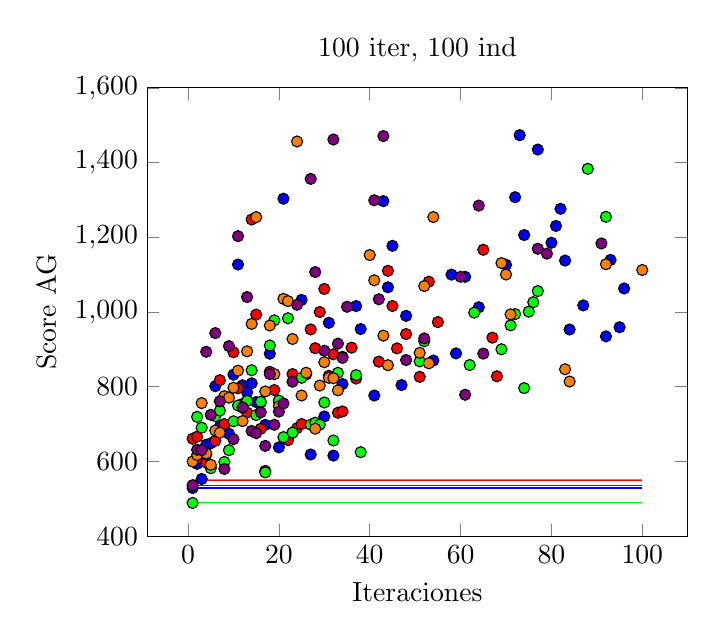
\begin{tikzpicture}
      \begin{axis}[
      title={100 iter, 100 ind},
      xlabel={Iteraciones},
      ylabel={Score AG},
      ymin=400,ymax=1600,
      ytick={400,600,...,1600}]
      
      \addplot[color=blue] coordinates {(1,528.986)(100,528.986)};
      \addplot[only marks, mark options={fill=blue}] coordinates {(1,528.986)(2,593.700)(3,553.090)(4,644.907)(5,648.794)(6,801.563)(7,693.969)(8,689.774)(9,674.341)(10,832.265)(11,1127.17)(12,803.969)(13,785.128)(14,809.254)(15,758.994)(16,758.101)(17,697.964)(18,888.463)(20,637.691)(21,1303.33)(23,676.504)(25,1032.60)(27,618.593)(30,720.479)(31,971.192)(32,615.736)(34,807.190)(37,1015.99)(38,954.341)(41,776.586)(43,1296.84)(44,1066.20)(45,1177.23)(47,804.531)(48,989.799)(54,870.108)(58,1100.17)(59,889.304)(61,1094.30)(64,1012.77)(70,1126.49)(72,1307.31)(73,1473.37)(74,1206.09)(77,1434.86)(80,1185.37)(81,1230.44)(82,1276.31)(83,1137.82)(84,953.222)(87,1017.70)(92,934.825)(93,1139.44)(95,959.294)(96,1063.09)};
      
      \addplot[color=red] coordinates {(1,549.068)(100,549.068)};
      \addplot[only marks, mark options={fill=red}] coordinates {(1,660.852)(2,666.407)(3,607.354)(4,597.262)(5,584.448)(6,655.193)(7,817.594)(8,700.118)(10,892.267)(11,795.962)(12,753.841)(13,730.861)(14,1247.67)(15,993.190)(16,687.347)(17,574.739)(18,839.997)(19,791.179)(20,758.977)(22,657.082)(23,833.915)(24,689.298)(25,700.211)(26,832.846)(27,953.467)(28,903.138)(29,1000.04)(30,1061.77)(31,829.241)(32,886.808)(33,730.422)(34,733.919)(36,904.635)(37,821.969)(42,867.188)(44,1110.32)(45,1016.17)(46,902.660)(48,941.033)(51,826.523)(53,1081.19)(55,973.080)(65,1166.69)(67,931.424)(68,828.018)};
      
      \addplot[color=green] coordinates {(1,489.003)(100,489.003)};
      \addplot[only marks, mark options={fill=green}] coordinates {(1,489.003)(2,719.458)(3,690.396)(4,618.345)(5,581.957)(6,721.231)(7,736.115)(8,598.717)(9,630.206)(10,707.552)(11,749.746)(12,744.226)(13,762.232)(14,844.151)(15,724.241)(16,759.622)(17,570.862)(18,910.532)(19,977.839)(20,762.887)(21,665.111)(22,983.399)(23,677.311)(25,824.045)(27,698.372)(28,703.609)(29,698.458)(30,757.888)(32,656.138)(33,837.361)(34,880.210)(37,831.205)(38,624.752)(51,867.936)(52,921.905)(62,858.181)(63,998.387)(69,900.364)(71,964.402)(72,994.463)(74,796.303)(75,1001.00)(76,1026.43)(77,1056.06)(88,1383.36)(92,1254.82)};
      
      \addplot[color=orange] coordinates {(1,551.723)(100,551.723)};
      \addplot[only marks, mark options={fill=orange}] coordinates {(1,599.837)(2,617.374)(3,756.323)(4,621.629)(5,591.070)(6,682.802)(7,676.916)(8,774.893)(9,770.761)(10,797.273)(11,843.035)(12,708.102)(13,894.805)(14,968.270)(15,1254.01)(17,787.431)(18,963.927)(19,833.770)(20,747.877)(21,1035.32)(22,1029.26)(23,927.834)(24,1456.53)(25,776.618)(26,837.522)(28,687.743)(29,803.286)(30,865.668)(31,823.848)(32,822.897)(33,790.343)(40,1152.52)(41,1084.96)(43,936.811)(44,857.662)(51,890.722)(52,1069.57)(53,862.829)(54,1254.17)(69,1131.06)(70,1100.38)(71,993.743)(83,846.831)(84,813.944)(92,1128.09)(100,1112.53)};
      
      \addplot[color=violet] coordinates {(1,536.370)(100,536.370)};
      \addplot[only marks, mark options={fill=violet}] coordinates {(1,536.370)(2,631.569)(3,629.995)(4,893.565)(5,724.972)(6,943.634)(7,761.127)(8,580.023)(9,908.763)(10,659.684)(11,1203.03)(12,745.168)(13,1040.05)(14,681.734)(15,675.790)(16,731.466)(17,641.636)(18,834.035)(19,698.253)(20,733.418)(21,755.310)(23,813.524)(24,1019.47)(27,1356.35)(28,1107.04)(30,896.455)(32,1461.73)(33,915.409)(34,877.381)(35,1014.09)(41,1299.16)(42,1034.14)(43,1470.92)(48,871.488)(52,929.403)(60,1094.33)(61,778.601)(64,1284.92)(65,888.706)(77,1169.37)(79,1156.35)(91,1183.51)};

      \end{axis}
\end{tikzpicture}}
\end{subfigure}
\newline
\centering
% Figura 12
\begin{subfigure}[b]{0.43\textwidth}
\resizebox{\linewidth}{!}{
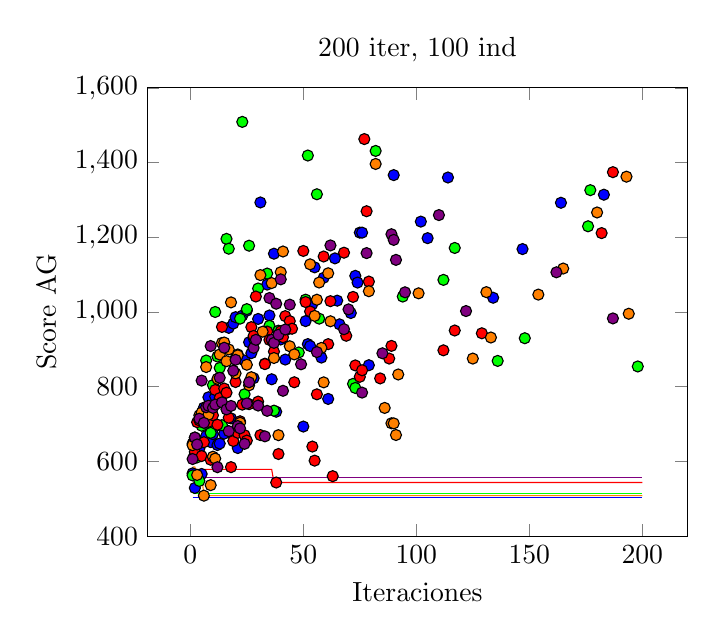
\begin{tikzpicture}
      \begin{axis}[
      title={200 iter, 100 ind},
      xlabel={Iteraciones},
      ylabel={Score AG},
      ymin=400,ymax=1600,
      ytick={400,600,...,1600}]
      
      \addplot[color=blue] coordinates {(1,504.006)(200,504.006)};
      \addplot[only marks, mark options={fill=blue}] coordinates {(1,568.263)(2,529.082)(3,612.791)(4,634.883)(5,566.537)(6,744.032)(7,668.199)(8,771.842)(9,651.837)(10,673.042)(11,773.983)(12,644.031)(13,647.959)(14,693.940)(15,674.484)(16,743.812)(17,957.715)(18,715.361)(19,969.138)(20,986.216)(21,636.007)(23,990.503)(24,870.267)(25,1003.61)(26,919.100)(27,889.964)(28,822.826)(30,981.507)(31,1293.30)(33,861.726)(34,1073.46)(35,990.742)(36,820.032)(37,1156.15)(38,733.190)(40,926.550)(42,872.804)(50,693.474)(51,975.670)(52,914.173)(53,909.029)(54,1021.25)(55,1119.64)(57,893.929)(58,878.104)(59,1091.68)(61,767.434)(64,1143.64)(65,1030.47)(66,967.110)(71,997.362)(73,1096.87)(74,1078.87)(75,1212.54)(76,1212.54)(79,857.651)(90,1366.51)(102,1242.03)(105,1197.73)(114,1360.11)(134,1038.27)(147,1168.51)(164,1292.45)(183,1314.07)};
      
      \addplot[color=green] coordinates {(1,513.151)(200,513.151)};
      \addplot[only marks, mark options={fill=green}] coordinates {(1,562.689)(2,619.136)(3,610.958)(4,547.841)(5,695.692)(6,711.006)(7,870.271)(8,725.372)(9,676.662)(10,804.429)(11,1000.18)(12,880.868)(13,850.350)(14,697.128)(15,790.605)(16,1195.83)(17,1169.50)(20,876.412)(21,886.399)(22,982.276)(23,1508.97)(24,780.107)(25,1007.79)(26,1177.56)(28,929.921)(29,928.681)(30,1062.99)(34,1103.00)(35,963.245)(37,736.039)(39,950.125)(43,953.462)(48,891.746)(51,1033.12)(52,1418.92)(56,1315.26)(57,982.355)(72,807.770)(73,796.800)(82,1431.25)(94,1041.42)(112,1086.06)(117,1171.52)(136,869.200)(148,929.901)(176,1229.52)(177,1326.22)(198,854.313)};
      
      \addplot[color=red] coordinates {(1,578.919)(36,578.919)(37,543.701)(200,543.701)};
      \addplot[only marks, mark options={fill=red}] coordinates {(1,647.826)(2,625.797)(3,705.175)(4,709.968)(5,614.520)(6,651.519)(7,715.514)(8,705.918)(9,604.603)(10,723.682)(11,791.295)(12,698.377)(13,769.661)(14,960.117)(15,795.191)(16,783.971)(17,717.143)(18,584.844)(19,654.755)(20,812.664)(21,676.754)(22,707.632)(23,752.132)(24,670.380)(25,655.875)(26,753.474)(27,959.591)(28,935.999)(29,1041.53)(30,760.227)(31,670.588)(33,860.645)(34,947.800)(35,925.404)(37,894.089)(38,543.701)(39,620.014)(40,948.538)(41,932.611)(42,989.057)(44,975.680)(45,955.351)(46,812.003)(50,1163.52)(51,1026.74)(53,1001.48)(54,639.886)(55,602.247)(56,779.721)(59,1148.63)(61,914.059)(62,1029.07)(63,560.697)(68,1158.87)(69,936.464)(72,1040.47)(73,857.094)(75,826.634)(76,844.145)(77,1462.95)(78,1269.80)(79,1081.54)(84,822.342)(88,875.486)(89,909.371)(112,897.510)(117,950.562)(129,943.155)(182,1211.28)(187,1374.40)};
      
      \addplot[color=orange] coordinates {(1,585.303)(2,585.303)(3,563.963)(5,563.963)(6,508.468)(200,508.468)};
      \addplot[only marks, mark options={fill=orange}] coordinates {(1,643.736)(2,663.912)(3,563.963)(4,723.569)(5,730.779)(6,508.468)(7,852.749)(8,725.253)(9,536.652)(10,612.789)(11,607.762)(12,821.124)(13,886.361)(14,917.265)(15,918.360)(16,868.428)(17,899.935)(18,1025.83)(20,835.835)(21,884.059)(22,703.434)(25,858.924)(26,803.894)(27,825.543)(31,1098.88)(32,947.438)(36,1077.58)(37,876.957)(39,670.408)(40,1106.61)(41,1162.00)(44,908.417)(46,886.687)(53,1127.70)(55,989.714)(56,1032.97)(57,1079.04)(58,904.006)(59,811.755)(61,1103.77)(62,975.251)(79,1055.70)(82,1396.35)(86,743.348)(89,702.245)(90,701.987)(91,670.871)(92,832.845)(101,1050.07)(125,875.448)(131,1053.23)(133,931.819)(154,1046.66)(165,1116.41)(180,1266.49)(193,1362.30)(194,995.452)};
      
      \addplot[color=violet] coordinates {(1,556.609)(200,556.609)};
      \addplot[only marks, mark options={fill=violet}] coordinates {(1,606.569)(2,664.157)(3,645.467)(4,714.586)(5,816.502)(6,703.307)(7,745.153)(8,749.152)(9,908.971)(10,743.476)(11,752.245)(12,584.661)(13,824.133)(14,758.178)(15,904.374)(16,739.366)(17,681.176)(18,748.668)(19,842.939)(20,872.126)(21,694.862)(22,688.517)(24,647.248)(25,755.465)(26,812.060)(28,904.103)(29,925.627)(30,749.720)(33,667.229)(34,735.485)(35,1037.45)(36,925.779)(37,917.511)(38,1022.23)(39,939.198)(40,1087.49)(41,789.158)(42,953.255)(44,1019.75)(49,860.129)(56,892.879)(62,1178.32)(68,954.005)(70,1007.12)(76,784.352)(78,1157.73)(85,889.592)(89,1208.29)(90,1193.10)(91,1139.59)(95,1052.84)(110,1259.52)(122,1002.63)(162,1106.36)(187,982.942)};
      
      \end{axis}
\end{tikzpicture}}
\end{subfigure}
\caption{Ejecuciones del modelo básico (100 ind.)}
\label{fig:basic_simulation_res_100}
\end{figure}

Finalmente, puede observarse en la figura \ref{fig:basic_model_results} el resultado obtenido correspondiente a la mejor ejecución obtenida utilizando el modelo básico, mostrándose centrado en la línea horizontal presente en la mitad de la imagen. Esta línea representa la aceleración o frenada que debería de aplicar un vehículo en cada uno de los instantes de la ruta, siendo el eje central, una aceleración equivalente a 0, es decir, no aplicar ninguna fuerza al vehículo. Tal y como se puede observar a simple vista, este resultado sería de poca utilidad si se llevase a cabo por un vehículo real, ya que no hay una apreciación de que con este comportamiento en un vehículo realmente se consiguiese ahorrar energía en esta ruta, y mucho menos, realizar una predicción del consumo que se asemejase a la de un vehículo real.

\begin{figure}[!htb]
    \centering
    \includegraphics[width=0.75\textwidth]{Modelo_Basico_Ruta.png}
    \caption{Resultado obtenido al utilizar el modelo básico}
    \label{fig:basic_model_results}
\end{figure}

Con todos estos resultados, se optó por, en lugar de intentar aplicar técnicas de mitigación de individuos erróneos o de suavizado de datos sobre este modelo, dar el paso hacia un modelo más avanzado, ya explicado anteriormente, y cuyos resultados se exponen en la siguiente sección.

\newpage
\section{Modelo avanzado}
Las primeras pruebas realizadas con este nuevo modelo se basan en la repetición de los casos utilizados para el modelo básico, es decir, a partir de la misma ruta inicial, repetir las diferentes combinaciones entre iteraciones y número de individuos. La métrica para la optimización utilizada por defecto inicialmente para las pruebas se centra en la mejora de los consumos eléctricos del vehículo, es decir, un sistema análogo al objetivo del modelo básico inicial.

En este caso, tal y como se explica en el capítulo "\nameref{Adv_AG}", existe también un valor para el margen entre puntos. Dado que la ruta inicial sobre la que se realizan las pruebas no es muy larga (aproximadamente 34 km), se deja el valor por defecto, 10 metros.

Las primeras ejecuciones, al igual que en el modelo básico, se trata de las combinaciones de 50, 100 y 200 iteraciones con una población total de 30 individuos. Como hecho a resaltar, tanto en estas gráficas como en las del modelo básico, se ha utilizado el mismo sistema a la hora de representar visualmente los datos, es decir, un punto por cada uno de los valores devueltos como mejor individuo en una iteración, y una línea siguiendo el mejor valor e individuo obtenido durante toda la ejecución del sistema.

Otra diferencia a destacar entre las gráficas mostradas en ambos modelos se trata de la escala utilizada en el eje Y de las mismas. En este caso, pese a tratarse también del valor de \textit{fitness} del algoritmo genético, este se asemeja más al valor del consumo que tendría un vehículo durante la ruta en vatios (W).

\begin{figure}[!htb]
% Figura 13
\begin{subfigure}[b]{0.43\textwidth}
\centering
\resizebox{\linewidth}{!}{
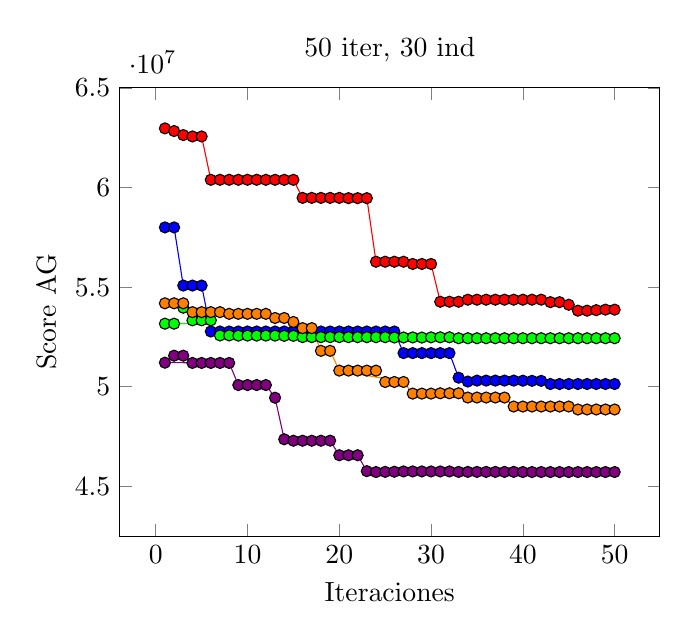
\begin{tikzpicture}
      \begin{axis}[
      title={50 iter, 30 ind},
      xlabel={Iteraciones},
      ylabel={Score AG},
      ymin=42500000,ymax=65000000]
      
      \addplot[color=blue] coordinates {(1,57997348)(2,57997348)(3,55078715)(5,55078715)(6,52773420)(19,52773420)(20,52773414)(26,52773414)(27,51688841)(32,51688841)(33,50456431)(34,50261877)(42,50261877)(43,50138136)(50,50138136)};
      \addplot[only marks, mark options={fill=blue}] coordinates {(1,57997348)(2,57997348)(3,55078715)(4,55078715)(5,55078715)(6,52773420)(7,52773420)(8,52773420)(9,52773420)(10,52773420)(11,52773420)(12,52773420)(13,52773420)(14,52773420)(15,52773420)(16,52773420)(17,52773420)(18,52773423)(19,52773423)(20,52773414)(21,52773414)(22,52773414)(23,52773415)(24,52773415)(25,52773415)(26,52773415)(27,51688841)(28,51688841)(29,51688841)(30,51688841)(31,51688841)(32,51688841)(33,50456431)(34,50261877)(35,50309132)(36,50309132)(37,50309132)(38,50309132)(39,50309132)(40,50304420)(41,50297834)(42,50296156)(43,50138136)(44,50138136)(45,50138136)(46,50138136)(47,50138136)(48,50138136)(49,50138136)(50,50138136)};
      
      \addplot[color=red] coordinates {(1,62966594)(2,62833385)(3,62630818)(4,62562171)(5,62562171)(6,60387623)(11,60387623)(12,60385729)(15,60385729)(16,59479465)(20,59479465)(21,59464553)(23,59464553)(24,56274960)(27,56274960)(28,56162937)(30,56162937)(31,54266980)(42,54266980)(43,54245981)(44,54245981)(45,54115480)(46,53819883)(50,53819883)};
      \addplot[only marks, mark options={fill=red}] coordinates {(1,62966594)(2,62833385)(3,62630818)(4,62562171)(5,62562171)(6,60387623)(7,60387623)(8,60387623)(9,60387623)(10,60387623)(11,60387655)(12,60385729)(13,60385729)(14,60385729)(15,60385729)(16,59479465)(17,59479465)(18,59479465)(19,59479465)(20,59479465)(21,59464553)(22,59464553)(23,59464553)(24,56274960)(25,56274960)(26,56274960)(27,56274960)(28,56162937)(29,56162937)(30,56162937)(31,54266980)(32,54266980)(33,54266980)(34,54369504)(35,54369504)(36,54369504)(37,54369504)(38,54369504)(39,54369504)(40,54369862)(41,54371382)(42,54371382)(43,54245981)(44,54245981)(45,54115480)(46,53819883)(47,53819883)(48,53844073)(49,53869724)(50,53869724)};
      
      \addplot[color=green] coordinates {(1,53165906)(6,53165906)(7,52574858)(8,52574858)(9,52565264)(13,52565264)(14,52555612)(15,52555612)(16,52491116)(20,52491116)(21,52487682)(25,52487682)(26,52472314)(27,52472033)(28,52472033)(29,52469568)(32,52469568)(33,52435331)(50,52435331)};
      \addplot[only marks, mark options={fill=green}] coordinates {(1,53165906)(2,53165906)(3,53966487)(4,53334657)(5,53334657)(6,53334657)(7,52574858)(8,52576959)(9,52565264)(10,52566748)(11,52566748)(12,52566748)(13,52566748)(14,52555612)(15,52555612)(16,52491116)(17,52491116)(18,52491116)(19,52491116)(20,52491116)(21,52487682)(22,52487682)(23,52487682)(24,52487682)(25,52487682)(26,52472314)(27,52472033)(28,52476228)(29,52469568)(30,52479338)(31,52481101)(32,52482684)(33,52435331)(34,52435331)(35,52435331)(36,52435331)(37,52435331)(38,52435331)(39,52435331)(40,52435639)(41,52435639)(42,52435639)(43,52435639)(44,52435673)(45,52435673)(46,52435673)(47,52435673)(48,52435673)(49,52435331)(50,52435331)};
      
      \addplot[color=orange] coordinates{(1,54188680)(3,54188680)(4,53744874)(7,53744874)(8,53660055)(12,53660055)(13,53451389)(14,53451389)(15,53250059)(16,52942711)(17,52942711)(18,51803047)(19,51803047)(20,50810593)(27,50239693)(28,49656729)(33,49656729)(34,49459193)(38,49459193)(39,49008020)(45,49008020)(46,48858472)(50,48858472)};
      \addplot[only marks, mark options={fill=orange}] coordinates {(1,54188680)(2,54188680)(3,54188680)(4,53744874)(5,53744874)(6,53744874)(7,53744874)(8,53660055)(9,53660055)(10,53660055)(11,53660055)(12,53660055)(13,53451389)(14,53451389)(15,53250059)(16,52942711)(17,52942711)(18,51803047)(19,51803047)(20,50810593)(21,50810593)(22,50810593)(23,50810593)(24,50810593)(25,50239693)(26,50239693)(27,50239693)(28,49656729)(29,49656729)(30,49656729)(31,49673013)(32,49673013)(33,49673013)(34,49459193)(35,49459193)(36,49459193)(37,49459193)(38,49459193)(39,49008020)(40,49008020)(41,49008020)(42,49008020)(43,49008020)(44,49008380)(45,49008380)(46,48858472)(47,48858472)(48,48858472)(49,48858472)(50,48858472)};
      
      \addplot[color=violet] coordinates {(1,51208062)(3,51208062)(4,51195733)(8,51195733)(9,50085896)(12,50085896)(13,49449949)(14,47364397)(15,47291436)(19,47291436)(20,46563247)(22,46563247)(23,45765011)(24,45719628)(50,45719628)};
      \addplot[only marks, mark options={fill=violet}] coordinates {(1,51208062)(2,51559457)(3,51559457)(4,51195733)(5,51195733)(6,51195733)(7,51195733)(8,51195733)(9,50085896)(10,50085896)(11,50085896)(12,50085896)(13,49449949)(14,47364397)(15,47291436)(16,47291436)(17,47291436)(18,47291436)(19,47296150)(20,46563247)(21,46563247)(22,46563247)(23,45765011)(24,45719628)(25,45728416)(26,45735754)(27,45750169)(28,45750169)(29,45750169)(30,45750169)(31,45750169)(32,45750169)(33,45727229)(34,45727229)(35,45727229)(36,45727229)(37,45727229)(38,45727229)(39,45729066)(40,45719628)(41,45719628)(42,45719628)(43,45719628)(44,45719628)(45,45719628)(46,45719628)(47,45719628)(48,45719628)(49,45720515)(50,45720978)};
      
      \end{axis}
\end{tikzpicture}}
\end{subfigure}
% Figura 14
\begin{subfigure}[b]{0.43\textwidth}
\resizebox{\linewidth}{!}{
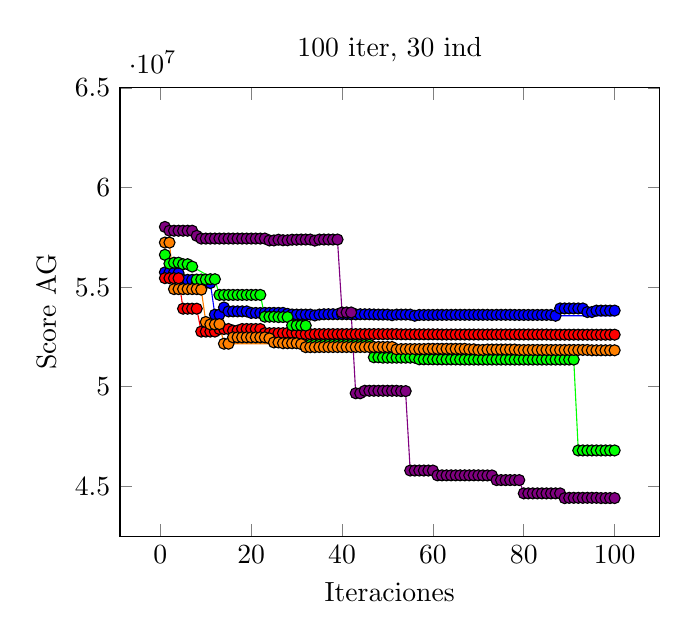
\begin{tikzpicture}
      \begin{axis}[
      title={100 iter, 30 ind},
      xlabel={Iteraciones},
      ylabel={Score AG},
      ymin=42500000,ymax=65000000]
      
      \addplot[color=blue] coordinates {(1,55741039)(2,55741039)(3,55731003)(4,55703195)(5,55366208)(7,55366208)(8,55205143)(11,55205143)(12,53618985)(33,53618985)(34,53579018)(55,53579018)(56,53563247)(100,53563247)};
      \addplot[only marks, mark options={fill=blue}] coordinates {(1,55741039)(2,55741039)(3,55731003)(4,55703195)(5,55366208)(6,55366208)(7,55366208)(8,55205143)(9,55205143)(10,55205143)(11,55205143)(12,53618985)(13,53618985)(14,53979662)(15,53783025)(16,53783025)(17,53783025)(18,53783025)(19,53783025)(20,53705143)(21,53705143)(22,53700455)(23,53707256)(24,53707256)(25,53707256)(26,53707256)(27,53707256)(28,53657995)(29,53626723)(30,53623615)(31,53623615)(32,53622510)(33,53622911)(34,53579018)(35,53623349)(36,53637312)(37,53640775)(38,53640775)(39,53640775)(40,53640775)(41,53640775)(42,53632417)(43,53632417)(44,53638256)(45,53636779)(46,53636779)(47,53628149)(48,53621829)(49,53621829)(50,53621829)(51,53592128)(52,53621829)(53,53621829)(54,53621829)(55,53621836)(56,53563247)(57,53604659)(58,53604659)(59,53604659)(60,53604659)(61,53608722)(62,53608722)(63,53608722)(64,53608722)(65,53611030)(66,53611030)(67,53611030)(68,53611030)(69,53611030)(70,53611030)(71,53611030)(72,53611030)(73,53605447)(74,53611030)(75,53611030)(76,53611031)(77,53611031)(78,53604593)(79,53604593)(80,53604593)(81,53604593)(82,53604593)(83,53605715)(84,53605715)(85,53605715)(86,53605716)(87,53563247)(88,53930098)(89,53930098)(90,53930098)(91,53930098)(92,53930098)(93,53930098)(94,53750055)(95,53750055)(96,53821788)(97,53821788)(98,53821788)(99,53821788)(100,53822645)};
      
      \addplot[color=red] coordinates {(1,55450757)(2,55450757)(3,55445387)(4,55445387)(5,53917519)(8,53917519)(9,52769361)(22,52769361)(23,52688877)(52,52641677)(53,52630107)(61,52630107)(62,52622989)(63,52622940)(67,52622940)(68,52622912)(69,52622867)(85,52622867)(86,52614650)(94,52614650)(95,52612509)(100,52612509)};
      \addplot[only marks, mark options={fill=red}] coordinates {(1,55450757)(2,55450757)(3,55445387)(4,55445387)(5,53917519)(6,53917519)(7,53917519)(8,53917519)(9,52769361)(10,52769361)(11,52769361)(12,52769361)(13,52897579)(14,52897579)(15,52897579)(16,52818196)(17,52818196)(18,52897615)(19,52897615)(20,52897615)(21,52897615)(22,52897846)(23,52688877)(24,52688877)(25,52688877)(26,52688877)(27,52688877)(28,52698875)(29,52698875)(30,52698888)(31,52641677)(32,52641677)(33,52641677)(34,52641677)(35,52641677)(36,52641677)(37,52641677)(38,52641677)(39,52641677)(40,52641677)(41,52641677)(42,52641677)(43,52641677)(44,52641677)(45,52641813)(46,52641813)(47,52641813)(48,52641813)(49,52641814)(50,52641819)(51,52641820)(52,52641820)(53,52630107)(54,52630107)(55,52630107)(56,52630107)(57,52630115)(58,52630142)(59,52630142)(60,52630142)(61,52630142)(62,52622989)(63,52622940)(64,52622940)(65,52622940)(66,52622940)(67,52622940)(68,52622912)(69,52622867)(70,52622867)(71,52622867)(72,52622867)(73,52622867)(74,52622867)(75,52622867)(76,52622875)(77,52622875)(78,52622875)(79,52622875)(80,52622875)(81,52622875)(82,52622875)(83,52622875)(84,52622876)(85,52622876)(86,52614650)(87,52614650)(88,52614650)(89,52614650)(90,52614670)(91,52614670)(92,52614670)(93,52614670)(94,52614670)(95,52612509)(96,52612509)(97,52612509)(98,52612818)(99,52613461)(100,52613461)};
      
      \addplot[color=green] coordinates {(1,56622022)(2,56178132)(4,56178132)(5,56149601)(6,56149601)(7,56031850)(12,55379550)(13,54610356)(22,54610356)(23,53515841)(25,53515841)(26,53497792)(28,53497792)(29,53076124)(31,53076124)(32,53069526)(33,52109174)(43,52109174)(44,52106663)(46,52106663)(47,51479841)(48,51479841)(49,51461199)(56,51461199)(57,51376564)(60,51376564)(61,51373209)(63,51373209)(64,51371880)(65,51371064)(66,51366217)(67,51365453)(74,51365453)(75,51364873)(77,51364873)(78,51363233)(91,51363233)(92,46804039)(100,46804039)};
      \addplot[only marks, mark options={fill=green}] coordinates {(1,56622022)(2,56178132)(3,56225517)(4,56225517)(5,56149601)(6,56149601)(7,56031850)(8,55379550)(9,55379550)(10,55379550)(11,55396760)(12,55396760)(13,54610356)(14,54610356)(15,54610356)(16,54610356)(17,54610356)(18,54610356)(19,54610356)(20,54610356)(21,54610356)(22,54610356)(23,53515841)(24,53515841)(25,53515841)(26,53497792)(27,53497792)(28,53497792)(29,53076124)(30,53076124)(31,53076124)(32,53069526)(33,52109174)(34,52109174)(35,52109174)(36,52109174)(37,52109174)(38,52109174)(39,52109174)(40,52109174)(41,52109174)(42,52109174)(43,52109174)(44,52106663)(45,52106663)(46,52106663)(47,51479841)(48,51479841)(49,51461199)(50,51461199)(51,51461199)(52,51461199)(53,51461199)(54,51461199)(55,51461199)(56,51461199)(57,51376564)(58,51376564)(59,51376564)(60,51376564)(61,51373209)(62,51373209)(63,51373209)(64,51371880)(65,51371064)(66,51366217)(67,51365453)(68,51365453)(69,51365453)(70,51365453)(71,51365453)(72,51365453)(73,51365453)(74,51365453)(75,51364873)(76,51364873)(77,51364873)(78,51363233)(79,51364877)(80,51364877)(81,51364877)(82,51364877)(83,51364252)(84,51364356)(85,51364356)(86,51364356)(87,51364356)(88,51364356)(89,51364357)(90,51364357)(91,51364357)(92,46804039)(93,46804039)(94,46804039)(95,46804039)(96,46804039)(97,46804039)(98,46804039)(99,46804039)(100,46804039)};
      
      \addplot[color=orange] coordinates{(1,57236375)(2,57236375)(3,54901427)(8,54901427)(9,54875092)(10,53249288)(13,53128888)(14,52160942)(30,52160942)(31,52139687)(32,51987435)(51,51987435)(52,51877840)(69,51877840)(70,51846677)(78,51846677)(79,51845494)(94,51845494)(95,51830398)(100,51830398)};
      \addplot[only marks, mark options={fill=orange}] coordinates {(1,57236375)(2,57236375)(3,54901427)(4,54901427)(5,54901427)(6,54901427)(7,54901427)(8,54901427)(9,54875092)(10,53249288)(11,53128888)(12,53128888)(13,53145280)(14,52160942)(15,52160942)(16,52479827)(17,52479827)(18,52479827)(19,52479827)(20,52479827)(21,52479827)(22,52479827)(23,52479827)(24,52427821)(25,52224160)(26,52224160)(27,52185435)(28,52185435)(29,52185435)(30,52185435)(31,52139687)(32,51987435)(33,51987435)(34,51987435)(35,51994303)(36,51994303)(37,51994303)(38,51994303)(39,51994395)(40,51994395)(41,51994395)(42,51994417)(43,51994895)(44,51994895)(45,51994895)(46,51994895)(47,51994895)(48,51994895)(49,51994895)(50,51994895)(51,51994895)(52,51877840)(53,51890940)(54,51890940)(55,51890940)(56,51890940)(57,51890940)(58,51890940)(59,51903417)(60,51903417)(61,51903417)(62,51903417)(63,51903417)(64,51903417)(65,51903417)(66,51902192)(67,51902737)(68,51878515)(69,51878515)(70,51846677)(71,51850682)(72,51868450)(73,51868450)(74,51868450)(75,51868450)(76,51868450)(77,51868450)(78,51868457)(79,51845494)(80,51845494)(81,51845494)(82,51847450)(83,51847450)(84,51847450)(85,51847450)(86,51847450)(87,51847450)(88,51847540)(89,51847540)(90,51847540)(91,51847540)(92,51847540)(93,51847540)(94,51847540)(95,51830398)(96,51830398)(97,51830398)(98,51830398)(99,51830398)(100,51830398)};
      
      \addplot[color=violet] coordinates {(1,58021712)(2,57831366)(7,57831366)(8,57574546)(9,57437023)(23,57437023)(24,57343824)(33,57343824)(34,57333339)(39,57333339)(40,53728297)(42,53728297)(43,49672437)(54,49672437)(55,45795194)(60,45795194)(61,45553308)(70,45553308)(71,45549632)(73,45549632)(74,45315817)(79,45315817)(80,44648894)(88,44648894)(89,44410423)(100,44410423)};
      \addplot[only marks, mark options={fill=violet}] coordinates {(1,58021712)(2,57831366)(3,57831366)(4,57831366)(5,57831366)(6,57831366)(7,57831366)(8,57574546)(9,57437023)(10,57437023)(11,57437023)(12,57437023)(13,57437449)(14,57437449)(15,57437449)(16,57437449)(17,57437449)(18,57437449)(19,57437449)(20,57437449)(21,57437449)(22,57437449)(23,57437449)(24,57343824)(25,57343824)(26,57380195)(27,57351865)(28,57351865)(29,57380195)(30,57380195)(31,57388762)(32,57388762)(33,57388762)(34,57333339)(35,57388762)(36,57388762)(37,57388762)(38,57388762)(39,57388762)(40,53728297)(41,53728297)(42,53728297)(43,49672437)(44,49672437)(45,49799349)(46,49799349)(47,49799349)(48,49799349)(49,49799349)(50,49799349)(51,49799349)(52,49799349)(53,49781395)(54,49781395)(55,45795194)(56,45795194)(57,45795194)(58,45795194)(59,45795194)(60,45795194)(61,45553308)(62,45553308)(63,45553308)(64,45553308)(65,45554302)(66,45554302)(67,45554302)(68,45554302)(69,45554302)(70,45554302)(71,45549632)(72,45549632)(73,45549632)(74,45315817)(75,45315817)(76,45315817)(77,45315817)(78,45315817)(79,45315817)(80,44648894)(81,44648894)(82,44648894)(83,44648894)(84,44648894)(85,44648894)(86,44648894)(87,44648894)(88,44648894)(89,44410423)(90,44426431)(91,44426431)(92,44426431)(93,44426431)(94,44426431)(95,44426431)(96,44426431)(97,44413128)(98,44413128)(99,44413128)(100,44413128)};
      
      \end{axis}
\end{tikzpicture}}
\end{subfigure}
\newline
\centering
% Figura 15
\begin{subfigure}[b]{0.43\textwidth}
\resizebox{\linewidth}{!}{
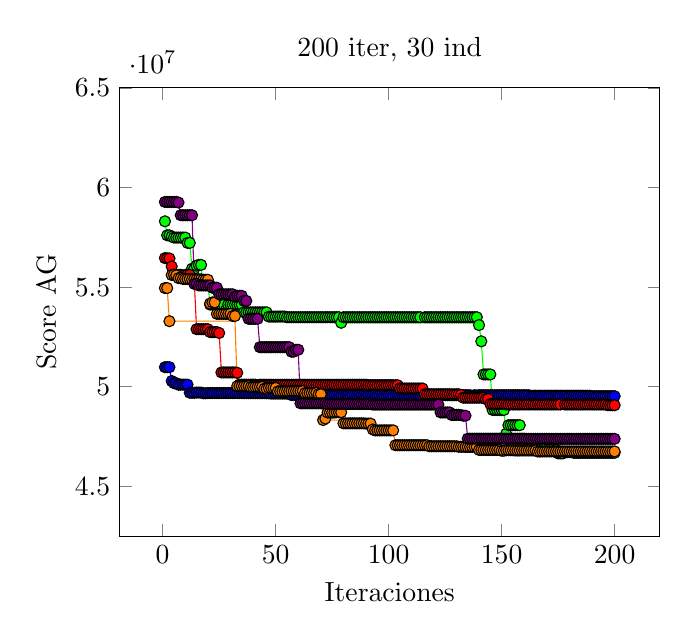
\begin{tikzpicture}
      \begin{axis}[
      title={200 iter, 30 ind},
      xlabel={Iteraciones},
      ylabel={Score AG},
      ymin=42500000,ymax=65000000]
      
      \addplot[color=blue] coordinates {(1,50981632)(3,50981632)(4,50288050)(5,50180571)(6,50180235)(7,50100596)(11,50100596)(12,49698639)(17,49698639)(18,49671276)(47,49671276)(48,49656660)(56,49656660)(57,49581229)(68,49581229)(69,49579172)(102,49579172)(103,49575126)(121,49575126)(122,49556458)(136,49556458)(137,49549219)(162,49549219)(163,49541348)(189,49541348)(190,49526688)(200,49526688)};
      \addplot[only marks, mark options={fill=blue}] coordinates {(1,50981632)(2,50981632)(3,50981632)(4,50288050)(5,50180571)(6,50180235)(7,50100596)(8,50106111)(9,50106111)(10,50106111)(11,50106111)(12,49698639)(13,49698639)(14,49698639)(15,49707515)(16,49707515)(17,49707515)(18,49671276)(19,49671276)(20,49682145)(21,49682145)(22,49682145)(23,49682145)(24,49682150)(25,49682150)(26,49682150)(27,49682154)(28,49682154)(29,49682154)(30,49682154)(31,49682154)(32,49682154)(33,49682154)(34,49682154)(35,49682154)(36,49677729)(37,49677729)(38,49677729)(39,49677729)(40,49677729)(41,49677729)(42,49677729)(43,49677729)(44,49677729)(45,49677729)(46,49671463)(47,49671463)(48,49656660)(49,49656660)(50,49656760)(51,49656760)(52,49656760)(53,49656760)(54,49656760)(55,49656760)(56,49656760)(57,49581229)(58,49581229)(59,49581229)(60,49581229)(61,49581229)(62,49581229)(63,49581229)(64,49581229)(65,49581229)(66,49581229)(67,49581229)(68,49581229)(69,49579172)(70,49579172)(71,49579215)(72,49579215)(73,49579466)(74,49579466)(75,49579466)(76,49579466)(77,49579466)(78,49579466)(79,49579466)(80,49579466)(81,49579466)(82,49579466)(83,49579466)(84,49579466)(85,49579466)(86,49579466)(87,49579466)(88,49579466)(89,49579466)(90,49579466)(91,49579466)(92,49579466)(93,49579466)(94,49579466)(95,49579466)(96,49579466)(97,49579466)(98,49579466)(99,49579466)(100,49579466)(101,49579466)(102,49579466)(103,49575126)(104,49576048)(105,49576048)(106,49576048)(107,49576048)(108,49576048)(109,49576048)(110,49576048)(111,49576048)(112,49576048)(113,49576048)(114,49576048)(115,49576048)(116,49576048)(117,49576048)(118,49576048)(119,49576048)(120,49576048)(121,49576048)(122,49556458)(123,49576048)(124,49576048)(125,49576048)(126,49576048)(127,49576048)(128,49574352)(129,49574352)(130,49574352)(131,49574352)(132,49574352)(133,49574460)(134,49574460)(135,49574460)(136,49574460)(137,49549219)(138,49574460)(139,49564276)(140,49574460)(141,49574460)(142,49574460)(143,49574460)(144,49574460)(145,49574460)(146,49574460)(147,49574460)(148,49574460)(149,49574460)(150,49574460)(151,49574460)(152,49574460)(153,49574460)(154,49574460)(155,49574460)(156,49574460)(157,49574460)(158,49574460)(159,49574460)(160,49574460)(161,49574460)(162,49574460)(163,49541348)(164,49549406)(165,49549406)(166,49549406)(167,49549406)(168,49549406)(169,49549406)(170,49549406)(171,49549406)(172,49549406)(173,49549406)(174,49549406)(175,49549406)(176,49549406)(177,49549406)(178,49549406)(179,49549406)(180,49549406)(181,49549406)(182,49549406)(183,49549406)(184,49549406)(185,49549406)(186,49549406)(187,49549406)(188,49549406)(189,49549406)(190,49526688)(191,49527119)(192,49527119)(193,49527119)(194,49527582)(195,49527582)(196,49527582)(197,49527582)(198,49527582)(199,49527585)(200,49527585)};
      
      \addplot[color=green] coordinates {(1,58301702)(2,57599724)(3,57599724)(4,57538477)(5,57486627)(10,57486627)(11,57220115)(12,57220115)(13,55927018)(17,55927018)(18,55196374)(19,55196374)(20,55160146)(21,54121883)(27,54121883)(28,53838474)(35,53838474)(36,53733241)(46,53733241)(47,53519514)(54,53519514)(55,53489145)(78,53489145)(79,53210554)(139,53210554)(140,53095570)(141,52279594)(142,50618682)(145,50618682)(146,48835725)(147,48835725)(148,48834528)(151,48834528)(152,47639620)(158,47639620)(159,47158078)(165,47158078)(166,47144074)(168,47144074)(169,46967896)(170,46967896)(171,46902685)(173,46902685)(174,46828283)(175,46654489)(200,46654489)};
      \addplot[only marks, mark options={fill=green}] coordinates {(1,58301702)(2,57599724)(3,57599724)(4,57538477)(5,57486627)(6,57486627)(7,57486627)(8,57486627)(9,57486627)(10,57486627)(11,57220115)(12,57220115)(13,55927018)(14,55927018)(15,56078619)(16,56115492)(17,56115492)(18,55196374)(19,55196374)(20,55160146)(21,54121883)(22,54121883)(23,54121883)(24,54121883)(25,54121883)(26,54121883)(27,54121883)(28,53838474)(29,54121883)(30,54121883)(31,54121883)(32,54121883)(33,54122267)(34,54122267)(35,54122274)(36,53733241)(37,53733241)(38,53733241)(39,53733241)(40,53733241)(41,53733241)(42,53733241)(43,53733241)(44,53733241)(45,53733241)(46,53733241)(47,53519514)(48,53519514)(49,53519514)(50,53519514)(51,53522699)(52,53522699)(53,53522699)(54,53522699)(55,53489145)(56,53489145)(57,53489145)(58,53489145)(59,53489145)(60,53489145)(61,53489149)(62,53489149)(63,53489149)(64,53489149)(65,53489149)(66,53489149)(67,53489149)(68,53489149)(69,53489149)(70,53489149)(71,53489149)(72,53489149)(73,53489149)(74,53489149)(75,53489149)(76,53489149)(77,53489149)(78,53489149)(79,53210554)(80,53489149)(81,53489149)(82,53489149)(83,53489149)(84,53489149)(85,53489149)(86,53489149)(87,53489149)(88,53489149)(89,53489149)(90,53489149)(91,53489149)(92,53489149)(93,53489149)(94,53489149)(95,53489149)(96,53489149)(97,53489149)(98,53489149)(99,53489149)(100,53489149)(101,53489149)(102,53489149)(103,53489149)(104,53489149)(105,53489149)(106,53489149)(107,53489149)(108,53489149)(109,53489149)(110,53489149)(111,53489149)(112,53489149)(113,53489149)(114,53489149)(115,5348919)(116,53489149)(117,53489149)(118,53489149)(119,53489149)(120,53489149)(121,53489149)(122,53489149)(123,53489149)(124,53489149)(125,53489149)(126,53489149)(127,53489149)(128,53489149)(129,53489149)(130,53489149)(131,53489149)(132,53489149)(133,53489149)(134,53489149)(135,53489149)(136,53489149)(137,53489149)(138,53489149)(139,53489149)(140,53095570)(141,52279594)(142,50618682)(143,50618682)(144,50618682)(145,50618682)(146,48835725)(147,48835725)(148,48834528)(149,48834528)(150,48834528)(151,48834578)(152,47639620)(153,48070842)(154,48070842)(155,48070842)(156,48070842)(157,48070842)(158,48070842)(159,47158078)(160,47158078)(161,47158078)(162,47158078)(163,47158078)(164,47158078)(165,47158078)(166,47144074)(167,47144074)(168,47144074)(169,46967896)(170,46967896)(171,46902685)(172,46902685)(173,46902685)(174,46828283)(175,46654489)(176,46654489)(177,46654489)(178,46715660)(179,46715660)(180,46715660)(181,46715660)(182,46682914)(183,46682914)(184,46682914)(185,46682914)(186,46683025)(187,46683025)(188,46683025)(189,46683025)(190,46683025)(191,46683057)(192,46683057)(193,46683088)(194,46683088)(195,46683088)(196,46683088)(197,46683088)(198,46683088)(199,46683088)(200,46683088)};
      
      \addplot[color=red] coordinates {(1,56455389)(2,56442469)(3,56441772)(4,56036991)(5,55616211)(8,55616211)(9,55589488)(12,55589488)(13,55383126)(14,55292970)(15,52888792)(20,52888792)(21,52743260)(22,52738421)(24,52738421)(25,52698178)(26,50718433)(32,50718433)(33,50700242)(34,50105278)(41,50105278)(42,50074878)(104,50074878)(105,49916591)(106,49913419)(107,49913187)(115,49913187)(116,49623086)(127,49623086)(128,49621018)(131,49621018)(132,49590507)(133,49450803)(142,49450803)(143,49385167)(144,49385167)(145,49130685)(151,49130685)(152,49111218)(176,49111218)(177,49110666)(196,49110666)(197,49072803)(200,49072803)};
      \addplot[only marks, mark options={fill=red}] coordinates {(1,56455389)(2,56442469)(3,56441772)(4,56036991)(5,55616211)(6,55616211)(7,55616211)(8,55616211)(9,55589488)(10,55611689)(11,55611689)(12,55611689)(13,55383126)(14,55292970)(15,52888792)(16,52888792)(17,52888792)(18,52888792)(19,52888792)(20,52888792)(21,52743260)(22,52738421)(23,52743308)(24,52743308)(25,52698178)(26,50718433)(27,50718433)(28,50718433)(29,50718433)(30,50719236)(31,50719236)(32,50719261)(33,50700242)(34,50105278)(35,50105278)(36,50105278)(37,50105278)(38,50105278)(39,50105278)(40,50105278)(41,50105278)(42,50074878)(43,50101940)(44,50101173)(45,50101173)(46,50099528)(47,50099528)(48,50099528)(49,50099434)(50,50099434)(51,50099470)(52,50099470)(53,50099470)(54,50099470)(55,50099470)(56,50099470)(57,50099470)(58,50099470)(59,50099470)(60,50099470)(61,50099470)(62,50099470)(63,50099470)(64,50099470)(65,50099470)(66,50099470)(67,50099470)(68,50099470)(69,50099470)(70,50099470)(71,50099470)(72,50099470)(73,50099470)(74,50099470)(75,50099470)(76,50099470)(77,50099470)(78,50099470)(79,50099470)(80,50099470)(81,50099470)(82,50099470)(83,50099470)(84,50099470)(85,50099470)(86,50099470)(87,50099470)(88,50099470)(89,50099470)(90,50099470)(91,50079687)(92,50079687)(93,50079687)(94,50079687)(95,50079687)(96,50079872)(97,50079872)(98,50079872)(99,50079872)(100,50079872)(101,50079872)(102,50079872)(103,50074878)(104,50074878)(105,49916591)(106,49913419)(107,49913187)(108,49913187)(109,49913187)(110,49913187)(111,49913189)(112,49913189)(113,49913189)(114,49913189)(115,49913189)(116,49623086)(117,49623086)(118,49623086)(119,49623086)(120,49623086)(121,49623086)(122,49623086)(123,49623086)(124,49623086)(125,49623086)(126,49623086)(127,49623086)(128,49621018)(129,49621018)(130,49621018)(131,49621018)(132,49590507)(133,49450803)(134,49450803)(135,49450803)(136,49450803)(137,49450803)(138,49451895)(139,49451895)(140,49451895)(141,49451895)(142,49451895)(143,49385167)(144,49385167)(145,49130685)(146,49130685)(147,49130685)(148,49130685)(149,49130832)(150,49130832)(151,49130832)(152,49111218)(153,49111218)(154,49111218)(155,49111218)(156,49111218)(157,49111218)(158,49111218)(159,49111218)(160,49111218)(161,49111218)(162,49111218)(163,49111218)(164,49111218)(165,49111218)(166,49111218)(167,49111218)(168,49111218)(169,49111218)(170,49111218)(171,49111218)(172,49111218)(173,49111218)(174,49111218)(175,49111218)(176,49111218)(177,4911066)(178,49110666)(179,49110666)(180,49110666)(181,49110666)(182,49110666)(183,49110666)(184,49110666)(185,49110666)(186,49110666)(187,49110666)(188,49110666)(189,49110666)(190,49110666)(191,49110666)(192,49110666)(193,49110666)(194,49110666)(195,49110666)(196,49110666)(197,49072803)(198,49072803)(199,49072803)(200,49072803)};
      
      \addplot[color=orange] coordinates {(1,54952515)(2,54952515)(3,53289871)(32,53289871)(33,50031338)(38,50031338)(39,49984164)(44,49984164)(45,49901860)(50,49901860)(51,49769327)(62,49769327)(63,49687630)(68,49687630)(69,49624197)(70,49624197)(71,48328349)(79,48328349)(80,48163130)(89,48163130)(90,48150786)(92,48150786)(93,47855478)(94,47809279)(102,47809279)(103,47064441)(117,47064441)(118,47013884)(128,47013884)(129,47012018)(130,47012018)(131,46987413)(133,46987413)(134,46980648)(139,46980648)(140,46826796)(149,46826796)(150,46789865)(165,46789865)(166,46750741)(200,46750741)};
      \addplot[only marks, mark options={fill=orange}] coordinates {(1,54952515)(2,54952515)(3,53289871)(4,55607794)(5,55622849)(6,55589038)(7,55452372)(8,55448830)(9,55410194)(10,55410194)(11,55410597)(12,55414301)(13,55392105)(14,55392105)(15,55392105)(16,55392105)(17,55392105)(18,55368107)(19,55368107)(20,55368107)(21,54174983)(22,54233804)(23,54233804)(24,53658203)(25,53658203)(26,53658203)(27,53658203)(28,53658203)(29,53658203)(30,53658203)(31,53550929)(32,53550929)(33,50031338)(34,50031338)(35,50031338)(36,50031338)(37,50031338)(38,50031338)(39,49984164)(40,49984164)(41,49991712)(42,49991712)(43,49991712)(44,49991712)(45,49901860)(46,49901860)(47,49941890)(48,49941890)(49,49941890)(50,49941890)(51,49769327)(52,49769327)(53,49769327)(54,49769327)(55,49769327)(56,49769327)(57,49782629)(58,49782629)(59,49782629)(60,49782629)(61,49782629)(62,49782629)(63,49687630)(64,49687630)(65,49687630)(66,49687630)(67,49687630)(68,49687630)(69,49624197)(70,49624197)(71,48328349)(72,48402359)(73,48703745)(74,48703745)(75,48703745)(76,48703745)(77,48720072)(78,48720072)(79,48720072)(80,48163130)(81,48163130)(82,48163130)(83,48163130)(84,48163130)(85,48163130)(86,48163130)(87,48163130)(88,48163130)(89,48163130)(90,48150786)(91,48150786)(92,48150786)(93,47855478)(94,47809279)(95,47809279)(96,47809279)(97,47810591)(98,47810591)(99,47810591)(100,47810591)(101,47810591)(102,47810591)(103,47064441)(104,47064441)(105,47064441)(106,47064441)(107,47064441)(108,47064441)(109,47064441)(110,47066045)(111,47066045)(112,47066045)(113,47066045)(114,47066045)(115,47066206)(116,47066206)(117,47066206)(118,47013884)(119,47013884)(120,47013884)(121,47013884)(122,47013884)(123,47013884)(124,47013884)(125,47013884)(126,47013884)(127,47013884)(128,47013884)(129,47012018)(130,47012018)(131,46987413)(132,46987413)(133,46990058)(134,46980648)(135,46980648)(136,46980648)(137,46980648)(138,46980648)(139,46980648)(140,46826796)(141,46826796)(142,46826796)(143,46826796)(144,46826796)(145,46826796)(146,46826796)(147,46826796)(148,46826796)(149,46826796)(150,46789865)(151,46789865)(152,46814964)(153,46814964)(154,46814964)(155,46814964)(156,46802637)(157,46802637)(158,46802637)(159,46802637)(160,46802637)(161,46802637)(162,46802637)(163,46802637)(164,46802637)(165,46802935)(166,46750741)(167,46750741)(168,46750741)(169,46754885)(170,46754885)(171,46754885)(172,46754885)(173,46754886)(174,46754886)(175,46754886)(176,46754886)(177,46754886)(178,46754886)(179,46754886)(180,46754886)(181,46754886)(182,46754886)(183,46754886)(184,46754886)(185,46754886)(186,46754886)(187,46754886)(188,46754886)(189,46754886)(190,46754886)(191,46753666)(192,46753666)(193,46753666)(194,46753666)(195,46753666)(196,46753666)(197,46753666)(198,46753666)(199,46753666)(200,46753666)};
      
      \addplot[color=violet] coordinates {(1,59273996)(6,59273996)(7,59244328)(8,58607783)(13,58607783)(14,55160930)(15,55160930)(16,55084668)(21,55084668)(22,54970430)(24,54970430)(25,54638599)(31,54638599)(32,54523338)(35,54523338)(36,54311225)(37,54311225)(38,53409703)(42,53409703)(43,51984748)(56,51984748)(57,51759954)(60,51759954)(61,49167542)(72,49167542)(73,49128139)(92,49128139)(93,49105804)(101,49105804)(102,49105293)(122,49105293)(123,48710417)(127,48710417)(128,48577100)(131,48577100)(132,48576061)(133,48546917)(134,48546917)(135,47393800)(160,47393800)(161,47385297)(200,47385297)};
      \addplot[only marks, mark options={fill=violet}] coordinates {(1,59273996)(2,59273996)(3,59273996)(4,59273996)(5,59273996)(6,59277502)(7,59244328)(8,58607783)(9,58607783)(10,58607783)(11,58607783)(12,58608173)(13,58608173)(14,55160930)(15,55160930)(16,55084668)(17,55084668)(18,55084668)(19,55084668)(20,55084668)(21,55084668)(22,54970430)(23,54970430)(24,54970430)(25,54638599)(26,54638599)(27,54638599)(28,54638599)(29,54638599)(30,54638599)(31,54638605)(32,54523338)(33,54563834)(34,54563834)(35,54563834)(36,54311225)(37,54311225)(38,53409703)(39,53409703)(40,53409703)(41,53409703)(42,53409703)(43,51984748)(44,51984748)(45,51984748)(46,51984748)(47,51984748)(48,51985418)(49,51985418)(50,51985418)(51,51985418)(52,51985418)(53,51985418)(54,51985418)(55,51985418)(56,51985418)(57,51759954)(58,51759954)(59,51854341)(60,51854341)(61,49167542)(62,49167542)(63,49167542)(64,49167542)(65,49167542)(66,49167542)(67,49167542)(68,49167542)(69,49167542)(70,49167545)(71,49167550)(72,49167550)(73,49128139)(74,49128139)(75,49128139)(76,49128139)(77,49130702)(78,49135660)(79,49135895)(80,49135895)(81,49135895)(82,49135895)(83,49135895)(84,49135931)(85,49135931)(86,49135931)(87,49135931)(88,49135931)(89,49135947)(90,49135989)(91,49135994)(92,49135994)(93,49105804)(94,49105804)(95,49105804)(96,49105804)(97,49105804)(98,49105804)(99,49105804)(100,49106583)(101,49106583)(102,49105293)(103,49105293)(104,49105293)(105,49105293)(106,49105293)(107,49105293)(108,49105293)(109,49105293)(110,49105293)(111,49105293)(112,49105293)(113,49105293)(114,49105293)(115,49105293)(116,49105299)(117,49105302)(118,49105302)(119,49105302)(120,49105302)(121,49105302)(122,49105302)(123,48710417)(124,48710417)(125,48710417)(126,48710417)(127,48710417)(128,48577100)(129,48577100)(130,48591581)(131,48591581)(132,48576061)(133,48546917)(134,48546917)(135,47393800)(136,47393800)(137,47393800)(138,47393800)(139,47393800)(140,47393800)(141,47393800)(142,47394651)(143,47394651)(144,47394737)(145,47394810)(146,47394810)(147,47394810)(148,47394810)(149,47394831)(150,47394831)(151,47394831)(152,47394831)(153,47394831)(154,47394831)(155,47394831)(156,47394831)(157,47394831)(158,47394831)(159,47394831)(160,47394831)(161,47385297)(162,47385297)(163,47385297)(164,47385297)(165,47385297)(166,47385297)(167,47385297)(168,47385297)(169,47385297)(170,47385297)(171,47385297)(172,47385297)(173,47385297)(174,47385297)(175,47385297)(176,47385297)(177,47385297)(178,47385297)(179,47385297)(180,47385297)(181,47385297)(182,47385297)(183,47385297)(184,47385297)(185,47385297)(186,47385297)(187,47385297)(188,47385297)(189,47385297)(190,47385297)(191,47385297)(192,47385297)(193,47385297)(194,47385297)(195,47385297)(196,47385297)(197,47385297)(198,47385297)(199,47385297)(200,47385297)};
      
      \end{axis}
\end{tikzpicture}}
\end{subfigure}
\caption{Ejecuciones del modelo avanzado (30 ind.)}
\label{fig:adv_simulation_res_30}
\end{figure}

En la figura \ref{fig:adv_simulation_res_30} se puede ver la primera serie de ejecuciones realizadas con 30 individuos como población. El primer hecho a destacar en las mismas es como la dispersión de puntos que se veía en el modelo básico, debido a los diferentes individuos inválidos,  desaparece por completo con este nuevo modelo. Esto se debe al hecho de incluir una política de corrección de individuos, la cual, para estas ejecuciones, como se ha explicado anteriormente, reemplaza a los individuos que no son válidos en una iteración por nuevos individuos, en cuyo proceso de creación, una de las condiciones es la validez del mismo.

El gran hecho a destacar es como, con este modelo, los valores que se van obteniendo conforme avanza el número de iteraciones continúa descendiendo continuamente en lugar de incrementarse, como ocurría con el modelo expuesto inicialmente. Así, mientras que en el modelo anterior se consideraba casi como excepción el hecho de que el algoritmo fuera capaz de mejorar su puntuación inicial, aquí se produce el caso contrario. En todas las ejecuciones realizadas se puede ver como el mejor valor obtenido por el sistema mejora por lo menos varias veces durante la ejecución, sin importar el número de iteración en la que se encuentra.

\begin{table}[!htb]
    \centering
    \begin{tabular}{m{0.15\textwidth}*6c}
    \toprule
    \multirow{2}*{\textbf{Medida}} & \multicolumn{3}{c}{\textbf{Modelo básico}} & \multicolumn{3}{c}{\textbf{Modelo avanzado}} \\
     & \textbf{50 it.} & \textbf{100 it.} & \textbf{200 it.} & \textbf{50 it.} & \textbf{100 it.} & \textbf{200 it.} \\
    \midrule
    \textbf{Desviación típica} & 160,18 & 185,21 & 204,78 & 1516340,109 & 1366946,431 & 1609001,44 \\
    \textbf{Media} & 821,93 & 868,78 & 883,89 & 51943674,12 & 52293420,68 & 50153101,26 \\
    \textbf{Coeficiente de variación} & 19,49\% & 21,32\% & 23,17\% & 2,92\% & 2,61\% & 3,21\% \\
    \bottomrule
    \end{tabular}
    \caption{Valores de dispersión de los modelos (30 ind.)}
    \label{tab:adv_simulation_cv_30}
\end{table}

Una forma bastante directa de constatar esta mejora respecto al modelo original es a través del cálculo del coeficiente de variación a partir de los datos obtenidos con ambas pruebas. Estos resultados se pueden comprobar en la tabla \ref{tab:adv_simulation_cv_30}, donde se puede ver de forma clara como con el modelo avanzado el coeficiente de variación (en porcentaje) es de media aproximadamente un 18\% menor respecto al modelo básico inicial.

\begin{figure}[!htb]
% Figura 16
\begin{subfigure}[b]{0.43\textwidth}
\centering
\resizebox{\linewidth}{!}{
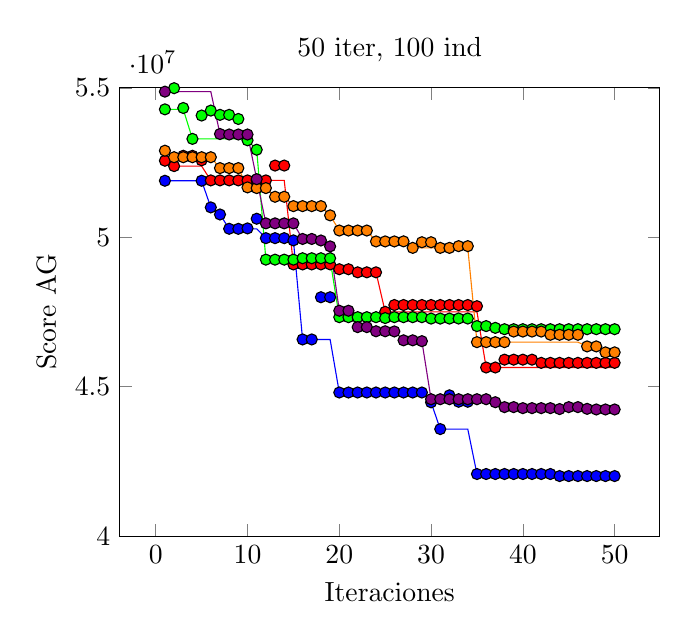
\begin{tikzpicture}
      \begin{axis}[
      title={50 iter, 100 ind},
      xlabel={Iteraciones},
      ylabel={Score AG},
      ymin=40000000,ymax=55000000]
      
      \addplot[color=blue] coordinates {(1,51892449)(5,51892449)(6,51000875)(7,50764126)(8,50285734)(9,50283434)(11,50283434)(12,49971857)(14,49971857)(15,49897775)(16,46582707)(19,46582707)(20,44807750)(29,44807750)(30,44479355)(31,43583463)(34,43583463)(35,42080470)(43,42080470)(44,42012213)(45,42012166)(46,42012166)(47,42011586)(50,42011586)};
      \addplot[only marks, mark options={fill=blue}] coordinates {(1,51892449)(5,51892449)(6,51000875)(7,50764126)(8,50285734)(9,50283434)(10,50298620)(11,50621603)(12,49971857)(13,49971857)(14,49971857)(15,49897775)(16,46582707)(17,46582707)(18,47995168)(19,47995168)(20,44807750)(21,44807750)(22,44807750)(23,44807750)(24,44807750)(25,44807750)(26,44807750)(27,44807750)(28,44807750)(29,44807750)(30,44479355)(31,43583463)(32,44713372)(33,44498108)(34,44498108)(35,42080470)(36,42080470)(37,42080470)(38,42080470)(39,42080470)(40,42080470)(41,42080470)(42,42080470)(43,42080470)(44,42012213)(45,42012166)(46,42012213)(47,42011586)(48,42012213)(49,42012212)(50,42011698)};
      
      \addplot[color=red] coordinates {(1,52562732)(2,52382371)(5,52382371)(6,51904500)(14,51904500)(15,49093248)(19,49093248)(20,48932056)(21,48932056)(22,48828427)(24,48828427)(25,47506836)(35,47506836)(36,45644361)(50,45644361)};
      \addplot[only marks, mark options={fill=red}] coordinates {(1,52562732)(2,52382371)(3,52727607)(4,52727607)(5,52577185)(6,51904500)(7,51904500)(8,51904500)(9,51904500)(10,51904500)(11,51904500)(12,51904500)(13,52400696)(14,52400696)(15,49093248)(16,49093248)(17,49093248)(18,49093248)(19,49093248)(20,48932056)(21,48932056)(22,48828427)(23,48828427)(24,48828427)(25,47506836)(26,47734441)(27,47734441)(28,47734441)(29,47734441)(30,47734441)(31,47734441)(32,47734441)(33,47734441)(34,47734441)(35,47695826)(36,45644361)(37,45644361)(38,45906774)(39,45906774)(40,45906774)(41,45906774)(42,45799975)(43,45799975)(44,45799975)(45,45799975)(46,45799975)(47,45799975)(48,45799975)(49,45799975)(50,45799989)};
      
      \addplot[color=green] coordinates {(1,54280957)(3,54280957)(4,53293386)(9,53293386)(10,53245740)(11,52930796)(12,49252889)(19,49252889)(20,47328073)(24,47328073)(25,47298661)(29,47298661)(30,47280933)(34,47280933)(35,47029249)(36,47029249)(37,46970345)(38,46925428)(50,46925428)};
      \addplot[only marks, mark options={fill=green}] coordinates {(1,54280957)(2,54989383)(3,54326661)(4,53293386)(5,54074973)(6,54240043)(7,54097418)(8,54097418)(9,53959471)(10,53245740)(11,52930796)(12,49252889)(13,49252889)(14,49252889)(15,49252889)(16,49299839)(17,49299839)(18,49299839)(19,49299839)(20,47328073)(21,47328073)(22,47328073)(23,47328073)(24,47328073)(25,47298661)(26,47328073)(27,47328073)(28,47328073)(29,47328073)(30,47280933)(31,47280933)(32,47280933)(33,47282870)(34,47282870)(35,47029249)(36,47029249)(37,46970345)(38,46925428)(39,46925428)(40,46925428)(41,46925428)(42,46925428)(43,46925428)(44,46925428)(45,46926154)(46,46926154)(47,46926173)(48,46926173)(49,46926173)(50,46926173)};
      
      \addplot[color=orange] coordinates{(1,52898080)(2,52680108)(6,52680108)(7,52315907)(9,52315907)(10,51670462)(11,51646954)(12,51646954)(13,51356623)(14,51356623)(15,51043322)(18,51043322)(19,50734099)(20,50226995)(23,50226995)(24,49862406)(27,49862406)(28,49646933)(30,49646933)(31,49646639)(34,49646639)(35,46492437)(46,46492437)(47,46349576)(48,46349576)(49,46150372)(50,46150372)};
      \addplot[only marks, mark options={fill=orange}] coordinates {(1,52898080)(2,52680108)(3,52680108)(4,52680108)(5,52680108)(6,52680108)(7,52315907)(8,52315907)(9,52315907)(10,51670462)(11,51646954)(12,51646954)(13,51356623)(14,51356623)(15,51043322)(16,51043322)(17,51043322)(18,51043322)(19,50734099)(20,50226995)(21,50226995)(22,50226995)(23,50226995)(24,49862406)(25,49862406)(26,49862406)(27,49864865)(28,49646933)(29,49835213)(30,49835213)(31,49646639)(32,49646639)(33,49704723)(34,49704723)(35,46492437)(36,46492437)(37,46492437)(38,46492437)(39,46846821)(40,46846821)(41,46846821)(42,46846821)(43,46739620)(44,46739620)(45,46739620)(46,46739620)(47,46349576)(48,46349576)(49,46150372)(50,46150372)};
      
      \addplot[color=violet] coordinates {(1,54873951)(6,54873951)(7,53456868)(8,53440332)(9,53440332)(10,53439467)(11,51945615)(12,50466994)(15,50466994)(16,49945099)(17,49945099)(18,49893665)(19,49696811)(20,47543627)(21,47543627)(22,46995141)(23,46995141)(24,46856509)(25,46856509)(26,46851226)(27,46553584)(28,46553584)(29,46525335)(30,44583266)(36,44583266)(37,44482452)(38,44318464)(39,44318464)(40,44284569)(43,44284569)(44,44253355)(47,44253355)(48,44239613)(50,44239613)};
      \addplot[only marks, mark options={fill=violet}] coordinates {(1,54873951)(2,55304855)(3,55304855)(4,55304855)(5,55304855)(6,55420601)(7,53456868)(8,53440332)(9,53440332)(10,53439467)(11,51945615)(12,50466994)(13,50466994)(14,50466994)(15,50466994)(16,49945099)(17,49945099)(18,49893665)(19,49696811)(20,47543627)(21,47543627)(22,46995141)(23,46995141)(24,46856509)(25,46856509)(26,46851226)(27,46553584)(28,46553584)(29,46525335)(30,44583266)(31,44583266)(32,44583266)(33,44583266)(34,44583266)(35,44583266)(36,44583266)(37,44482452)(38,44318464)(39,44318464)(40,44284569)(41,44284569)(42,44284569)(43,44284569)(44,44253355)(45,44318464)(46,44318464)(47,44260674)(48,44239613)(49,44239613)(50,44239613)};
      
      \end{axis}
\end{tikzpicture}}
\end{subfigure}
% Figura 17
\begin{subfigure}[b]{0.43\textwidth}
\resizebox{\linewidth}{!}{
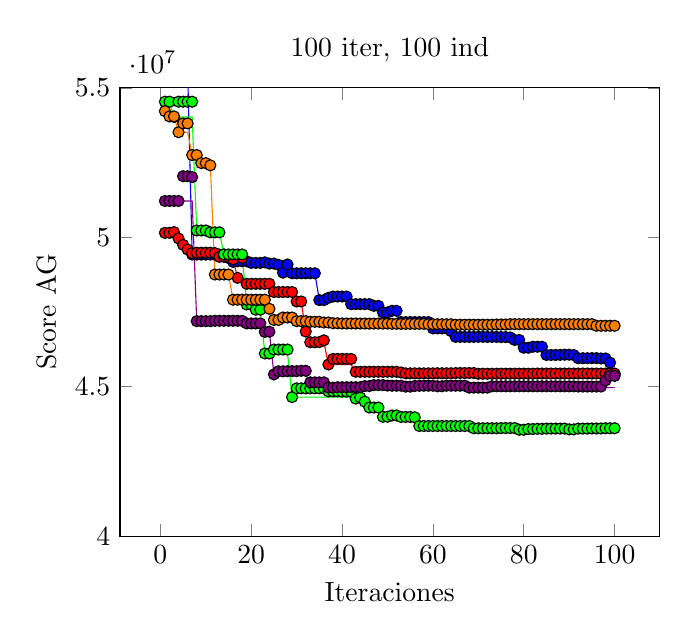
\begin{tikzpicture}
      \begin{axis}[
      title={100 iter, 100 ind},
      xlabel={Iteraciones},
      ylabel={Score AG},
      ymin=40000000,ymax=55000000]
      
      \addplot[color=blue] coordinates {(1,55970905)(2,55859331)(3,55859331)(4,55644000)(5,55644000)(6,55594626)(7,49421724)(14,49421724)(15,49307306)(16,49176813)(19,49176813)(20,49143995)(23,49143995)(24,49120673)(25,49120673)(26,49079662)(27,48818235)(28,48818235)(29,48796709)(34,48796709)(35,47898942)(41,47898942)(42,47764254)(46,47764254)(47,47706061)(48,47706061)(49,47485527)(52,47485527)(53,47164081)(59,47164081)(60,46952365)(63,46952365)(64,46861584)(65,46667664)(71,46667664)(72,46666836)(74,46666836)(75,46662057)(76,46662057)(77,46650280)(78,46565318)(79,46565318)(80,46305751)(84,46305751)(85,46063339)(90,46063339)(91,46060001)(92,45954330)(96,45954330)(97,45945945)(98,45945945)(99,45806693)(100,45429507)};
      \addplot[only marks, mark options={fill=blue}] coordinates {(1,55970905)(2,55859331)(3,55859331)(4,55644000)(5,55644000)(6,55594626)(7,49421724)(8,49421724)(9,49421724)(10,49421724)(11,49421724)(12,49421724)(13,49421724)(14,49421724)(15,49307306)(16,49176813)(17,49199130)(18,49199130)(19,49199130)(20,49143995)(21,49143995)(22,49143995)(23,49162177)(24,49120673)(25,49120673)(26,49079662)(27,48818235)(28,49091902)(29,48796709)(30,48796709)(31,48796709)(32,48796709)(33,48796709)(34,48796709)(35,47898942)(36,47898942)(37,47973755)(38,48018320)(39,48018320)(40,48018320)(41,48018320)(42,47764254)(43,47764254)(44,47764254)(45,47764254)(46,47764254)(47,47706061)(48,47706061)(49,47485527)(50,47485527)(51,47541040)(52,47541040)(53,47164081)(54,47164081)(55,47164081)(56,47164081)(57,47164081)(58,47164081)(59,47164081)(60,46952365)(61,46952365)(62,46952365)(63,46952365)(64,46861584)(65,46667664)(66,46667664)(67,46667664)(68,46667664)(69,46667664)(70,46670355)(71,46670355)(72,46666836)(73,46666836)(74,46666836)(75,46662057)(76,46662057)(77,46650280)(78,46565318)(79,46565318)(80,46305751)(81,46305751)(82,46338441)(83,46338441)(84,46338552)(85,46063339)(86,46063339)(87,46063339)(88,46067658)(89,46072552)(90,46072552)(91,46060001)(92,45954330)(93,45954330)(94,45954330)(95,45957829)(96,45957829)(97,45945945)(98,45945945)(99,45806693)(100,45429507)};
      
      \addplot[color=red] coordinates {(1,50148835)(3,50148835)(4,49961099)(5,49746684)(6,49591369)(7,49470845)(12,49470845)(13,49346217)(15,49346217)(16,49265405)(17,48643926)(18,48643926)(19,48443623)(24,48443623)(25,48169730)(29,48169730)(30,47854110)(31,47854110)(32,46847449)(33,46488694)(36,46488694)(37,45744260)(42,45744260)(43,45500648)(52,45500648)(53,45476899)(54,45448010)(69,45448010)(70,45434662)(100,45434662)};
      \addplot[only marks, mark options={fill=red}] coordinates {(1,50148835)(2,50148835)(3,50174001)(4,49961099)(5,49746684)(6,49591369)(7,49470845)(8,49485855)(9,49485855)(10,49485855)(11,49485855)(12,49471736)(13,49346217)(14,49346217)(15,49346217)(16,49265405)(17,48643926)(18,49314422)(19,48443623)(20,48443623)(21,48443623)(22,48443623)(23,48443623)(24,48443623)(25,48169730)(26,48169730)(27,48169730)(28,48169730)(29,48169730)(30,47854110)(31,47854110)(32,46847449)(33,46488694)(34,46488694)(35,46495688)(36,46553261)(37,45744260)(38,45930797)(39,45930797)(40,45930797)(41,45930797)(42,45930797)(43,45500648)(44,45500648)(45,45500648)(46,45500648)(47,45500648)(48,45500648)(49,45500648)(50,45500702)(51,45500702)(52,45500702)(53,45476899)(54,45448010)(55,45448010)(56,45448010)(57,45448010)(58,45448475)(59,45448475)(60,45448475)(61,45452452)(62,45450876)(63,45450876)(64,45451332)(65,45457898)(66,45459651)(67,45459651)(68,45459651)(69,45459651)(70,45434662)(71,45434662)(72,45434662)(73,45434662)(74,45437630)(75,45437630)(76,45437630)(77,45437630)(78,45438513)(79,45438513)(80,45438513)(81,45436213)(82,45436213)(83,45441754)(84,45441754)(85,45441754)(86,45441867)(87,45441867)(88,45441867)(89,45442017)(90,45442017)(91,45442433)(92,45443435)(93,45443435)(94,45443435)(95,45441842)(96,45441842)(97,45441225)(98,45441225)(99,45441225)(100,45441225)};
      
      \addplot[color=green] coordinates {(1,54537497)(2,54537497)(3,54025445)(7,54025445)(8,50228983)(10,50228983)(11,50166624)(13,50166624)(14,49427189)(18,49427189)(19,47753614)(20,47753614)(21,47577209)(22,47577209)(23,46114831)(28,46114831)(29,44654724)(42,44654724)(43,44603728)(44,44603728)(45,44500290)(46,44304198)(48,44304198)(49,43995680)(52,43995680)(53,43989356)(55,43989356)(56,43977271)(57,43686725)(68,43686725)(69,43611580)(78,43611580)(79,43561179)(100,43561179)};
      \addplot[only marks, mark options={fill=green}] coordinates {(1,54537497)(2,54537497)(3,54025445)(4,54537497)(5,54537497)(6,54537497)(7,54537497)(8,50228983)(9,50228983)(10,50228983)(11,50166624)(12,50166624)(13,50166624)(14,49427189)(15,49427189)(16,49427189)(17,49427189)(18,49427189)(19,47753614)(20,47753614)(21,47577209)(22,47577209)(23,46114831)(24,46114831)(25,46244894)(26,46244894)(27,46244894)(28,46244894)(29,44654724)(30,44947189)(31,44947189)(32,44947189)(33,44947189)(34,44947189)(35,44947189)(36,44947189)(37,44847677)(38,44847677)(39,44847677)(40,44836816)(41,44836816)(42,44836816)(43,44603728)(44,44638783)(45,44500290)(46,44304198)(47,44304198)(48,44304198)(49,43995680)(50,43995680)(51,44039626)(52,44039626)(53,43989356)(54,43989356)(55,43989356)(56,43977271)(57,43686725)(58,43686725)(59,43686725)(60,43686725)(61,43686725)(62,43686725)(63,43686725)(64,43686725)(65,43686725)(66,43686725)(67,43686725)(68,43686725)(69,43611580)(70,43611580)(71,43611580)(72,43611580)(73,43611580)(74,43611580)(75,43616920)(76,43617881)(77,43617881)(78,43617881)(79,43561179)(80,43561179)(81,43585102)(82,43585102)(83,43591826)(84,43591826)(85,43599839)(86,43599839)(87,43599839)(88,43599839)(89,43599839)(90,43573616)(91,43573616)(92,43599839)(93,43599839)(94,43599839)(95,43604766)(96,43604766)(97,43604766)(98,43612358)(99,43612358)(100,43612358)};
      
      \addplot[color=orange] coordinates{(1,54221345)(3,54044845)(4,53516368)(6,53516368)(7,52752842)(8,52752842)(9,52483170)(10,52483170)(11,52407364)(12,48755639)(15,48755639)(16,47912019)(22,47912019)(23,47911554)(24,47607171)(25,47235558)(29,47235558)(30,47195754)(32,47195754)(33,47173432)(35,47173432)(36,47149903)(37,47149903)(38,47126656)(39,47125637)(40,47117939)(41,47116855)(43,47116855)(44,47114035)(45,47114035)(46,47111526)(50,47111526)(51,47106496)(52,47106496)(53,47104301)(58,47104301)(59,47091855)(64,47091855)(65,47074968)(95,47074968)(96,47039766)(100,47039766)};
      \addplot[only marks, mark options={fill=orange}] coordinates {(1,54221345)(2,54044845)(3,54044845)(4,53516368)(5,53810966)(6,53810966)(7,52752842)(8,52752842)(9,52483170)(10,52483170)(11,52407364)(12,48755639)(13,48755639)(14,48755639)(15,48755639)(16,47912019)(17,47912019)(18,47912019)(19,47912019)(20,47912019)(21,47912019)(22,47912019)(23,47911554)(24,47607171)(25,47235558)(26,47235558)(27,47316384)(28,47316384)(29,47316384)(30,47195754)(31,47195754)(32,47195754)(33,47173432)(34,47173432)(35,47173432)(36,47149903)(37,47149903)(38,47126656)(39,47125637)(40,47117939)(41,47116855)(42,47116855)(43,47116855)(44,47114035)(45,47114896)(46,47111526)(47,47113122)(48,47113122)(49,47112917)(50,47112917)(51,47106496)(52,47106496)(53,47104301)(54,47104301)(55,47104367)(56,47104367)(57,47104367)(58,47104367)(59,47091855)(60,47091855)(61,47091855)(62,47091855)(63,47091855)(64,47091855)(65,47074968)(66,47074968)(67,47074968)(68,47074968)(69,47075150)(70,47075150)(71,47075150)(72,47075150)(73,47075150)(74,47082791)(75,47082791)(76,47082791)(77,47094503)(78,47094997)(79,47094997)(80,47094997)(81,47094997)(82,47094997)(83,47094997)(84,47095002)(85,47095077)(86,47095118)(87,47095118)(88,47095118)(89,47095126)(90,47095126)(91,47095145)(92,47095157)(93,47095157)(94,47095157)(95,47095157)(96,47039766)(97,47039766)(98,47039766)(99,47039766)(100,47040356)};
      
      \addplot[color=violet] coordinates {(1,51216317)(7,51216317)(8,47194826)(18,47194826)(19,47119693)(22,47119693)(23,46835128)(24,46835128)(25,45413049)(32,45413049)(33,45147014)(36,45147014)(37,44970528)(100,44970528)};
      \addplot[only marks, mark options={fill=violet}] coordinates {(1,51216317)(2,51216317)(3,51216317)(4,51216317)(5,52044039)(6,52044039)(7,52014422)(8,47194826)(9,47194826)(10,47194826)(11,47194826)(12,47207159)(13,47207159)(14,47207172)(15,47207175)(16,47207175)(17,47207175)(18,47203404)(19,47119693)(20,47119693)(21,47119693)(22,47119693)(23,46835128)(24,46843087)(25,45413049)(26,45517272)(27,45517272)(28,45521705)(29,45521705)(30,45521705)(31,45533905)(32,45533905)(33,45147014)(34,45147014)(35,45147014)(36,45147014)(37,44970528)(38,44970528)(39,44984419)(40,44984419)(41,44984419)(42,44984419)(43,44984419)(44,44984419)(45,45022072)(46,45022072)(47,45054429)(48,45054429)(49,45054429)(50,45038842)(51,45034683)(52,45034683)(53,45034683)(54,45003571)(55,45003571)(56,45026993)(57,45030764)(58,45034146)(59,45034687)(60,45034815)(61,45016901)(62,45016901)(63,45034815)(64,45034815)(65,45034664)(66,45034815)(67,45034815)(68,44970528)(69,44970528)(70,44970528)(71,44970528)(72,44970528)(73,45015663)(74,45015663)(75,45015663)(76,45015663)(77,45015663)(78,45015663)(79,45015663)(80,45015663)(81,45015672)(82,45015672)(83,45015672)(84,45015672)(85,45015672)(86,45015672)(87,45015672)(88,45015672)(89,45013434)(90,45013434)(91,45013434)(92,45006671)(93,45006671)(94,45006671)(95,45006671)(96,45006671)(97,45006671)(98,45209455)(99,45363507)(100,45363507)};
      
      \end{axis}
\end{tikzpicture}}
\end{subfigure}
\newline
\centering
% Figura 18
\begin{subfigure}[b]{0.43\textwidth}
\resizebox{\linewidth}{!}{
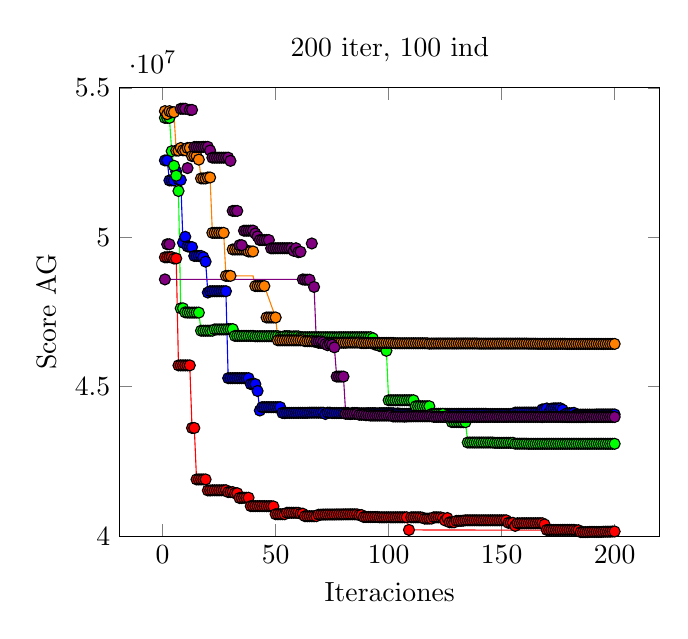
\begin{tikzpicture}
      \begin{axis}[
      title={200 iter, 100 ind},
      xlabel={Iteraciones},
      ylabel={Score AG},
      ymin=40000000,ymax=55000000]
      
      \addplot[color=blue] coordinates {(1,52572707)(2,52572707)(3,51903102)(8,51903102)(9,49820089)(10,49820089)(11,49696716)(12,49682450)(13,49672288)(14,49376673)(17,49376673)(18,49334100)(19,49185921)(20,48152945)(28,48152945)(29,45287286)(38,45287286)(39,45088542)(41,45088542)(42,44859002)(43,44205797)(52,44205797)(53,44125062)(54,44117186)(71,44117186)(72,44090022)(82,44090022)(83,44086346)(177,44086346)(178,44072364)(182,44072364)(183,44067407)(200,44067407)};
      \addplot[only marks, mark options={fill=blue}] coordinates {(1,52572707)(2,52572707)(3,51903102)(4,51903102)(5,51903102)(6,52197529)(7,51944268)(8,51918623)(9,49820089)(10,50017811)(11,49696716)(12,49682450)(13,49672288)(14,49376673)(15,49376673)(16,49376673)(17,49376673)(18,49334100)(19,49185921)(20,48152945)(21,48196055)(22,48196055)(23,48196055)(24,48196055)(25,48196055)(26,48196055)(27,48196055)(28,48196055)(29,45287286)(30,45287286)(31,45287286)(32,45287286)(33,45287286)(34,45287286)(35,45287286)(36,45287286)(37,45287286)(38,45287286)(39,45088542)(40,45088542)(41,45088542)(42,44859002)(43,44205797)(44,44317133)(45,44317133)(46,44317133)(47,44317133)(48,44317133)(49,44317133)(50,44317133)(51,44317133)(52,44317134)(53,44125062)(54,44117186)(55,44125062)(56,44125062)(57,44125693)(58,44125693)(59,44125693)(60,44125693)(61,44126628)(62,44126628)(63,44126628)(64,44126628)(65,44132277)(66,44132277)(67,44132277)(68,44132277)(69,44132277)(70,44132415)(71,44132415)(72,44090022)(73,44132448)(74,44132448)(75,44119689)(76,44119689)(77,44119689)(78,44119689)(79,44119689)(80,44121896)(81,44121896)(82,44121896)(83,44086346)(84,44123509)(85,44123509)(86,44123509)(87,44112126)(88,44112126)(89,44112126)(90,44112126)(91,44116641)(92,44116641)(93,44117221)(94,44117221)(95,44108719)(96,44117221)(97,44117221)(98,44117629)(99,44117629)(100,44117713)(101,44114387)(102,44114387)(103,44094917)(104,44109410)(105,44099438)(106,44094543)(107,44094543)(108,44094543)(109,44097069)(110,44097069)(111,44097069)(112,44097069)(113,44097069)(114,44097069)(115,44095310)(116,44095310)(117,44095310)(118,44095310)(119,44092620)(120,44092620)(121,44092620)(122,44092889)(123,44092889)(124,44092994)(125,44092994)(126,44092994)(127,44092994)(128,44092994)(129,44092994)(130,44092994)(131,44093220)(132,44093220)(133,44092540)(134,44092540)(135,44093982)(136,44093982)(137,44093982)(138,44093982)(139,44093982)(140,44093982)(141,44093982)(142,44093982)(143,44093982)(144,44086346)(145,44086346)(146,44086346)(147,44086346)(148,44086346)(149,44086346)(150,44086346)(151,44086346)(152,44086346)(153,44086346)(154,44086346)(155,44086346)(156,44135017)(157,44135017)(158,44135017)(159,44135017)(160,44136122)(161,44136122)(162,44136122)(163,44136122)(164,44136122)(165,44136122)(166,44136122)(167,44136122)(168,44242679)(169,44242679)(170,44273783)(171,44125903)(172,44267301)(173,44276946)(174,44276946)(175,44276946)(176,44278954)(177,44232231)(178,44072364)(179,44114783)(180,44114783)(181,44114783)(182,44126545)(183,44067407)(184,44067407)(185,44067407)(186,44067407)(187,44067407)(188,44067407)(189,44067407)(190,44067407)(191,44067407)(192,44074540)(193,44074540)(194,44074540)(195,44074540)(196,44074540)(197,44074540)(198,44074540)(199,44074540)(200,44074540)};
      
      \addplot[color=green] coordinates {(1,53996086)(3,53996086)(4,52881382)(5,52391887)(6,52062925)(7,51550156)(8,47623923)(9,47623923)(10,47489181)(11,47480932)(16,47480932)(17,46875408)(31,46875408)(32,46701421)(40,46701421)(41,46689715)(51,46689715)(52,46670823)(53,46669562)(54,46669562)(60,46669562)(61,46660713)(62,46656470)(76,46656470)(77,46653067)(92,46653067)(93,46621592)(94,46411298)(95,46411298)(96,46362571)(97,46349018)(98,46349018)(99,46203548)(100,44547833)(111,44547833)(112,44347258)(118,44347258)(119,44090086)(124,44090086)(125,44000639)(127,44000639)(128,43817272)(131,43817272)(132,43815179)(134,43815179)(135,43133718)(146,43133718)(147,43122954)(155,43122954)(156,43095325)(161,43095325)(162,43090433)(200,43090433)};
      \addplot[only marks, mark options={fill=green}] coordinates {(1,53996086)(2,53996086)(3,53996086)(4,52881382)(5,52391887)(6,52062925)(7,51550156)(8,47623923)(9,47623923)(10,47489181)(11,47480932)(12,47480932)(13,47480932)(14,47480932)(15,47480932)(16,47480932)(17,46875408)(18,46875408)(19,46875408)(20,46875408)(21,46875408)(22,46875408)(23,46918633)(24,46918633)(25,46918633)(26,46918633)(27,46918633)(28,46918633)(29,46928186)(30,46928186)(31,46928186)(32,46701421)(33,46701421)(34,46701421)(35,46701421)(36,46701421)(37,46701421)(38,46701421)(39,46701421)(40,46701421)(41,46689715)(42,46689715)(43,46691617)(44,46691617)(45,46691617)(46,46691617)(47,46691617)(48,46691617)(49,46691617)(50,46691617)(51,46691617)(52,46670823)(53,46669562)(54,46691617)(55,46691617)(56,46691617)(57,46679447)(58,46685494)(59,46685569)(60,46685569)(61,46660713)(62,46656470)(63,46656470)(64,46656470)(65,46656470)(66,46656470)(67,46656470)(68,46656470)(69,46656470)(70,46656470)(71,46656470)(72,46656470)(73,46656470)(74,46656470)(75,46656470)(76,46656472)(77,46653067)(78,46656472)(79,46656472)(80,46656472)(81,46656480)(82,46656480)(83,46656480)(84,46656480)(85,46656480)(86,46656480)(87,46656480)(88,46656480)(89,46656480)(90,46656480)(91,46656480)(92,46656480)(93,46621592)(94,46411298)(95,46411298)(96,46362571)(97,46349018)(98,46349018)(99,46203548)(100,44547833)(101,44547833)(102,44547833)(103,44547833)(104,44547833)(105,44547833)(106,44547833)(107,44548230)(108,44548230)(109,44548230)(110,44548235)(111,44548235)(112,44347258)(113,44347258)(114,44347258)(115,44347258)(116,44347258)(117,44347258)(118,44347679)(119,44090086)(120,44090086)(121,44090086)(122,44090086)(123,44090086)(124,44090086)(125,44000639)(126,44000639)(127,44000639)(128,43817272)(129,43817272)(130,43817272)(131,43817272)(132,43815179)(133,43815179)(134,43815179)(135,43133718)(136,43133718)(137,43133718)(138,43133718)(139,43133718)(140,43133718)(141,43133718)(142,43133718)(143,43133739)(144,43133739)(145,43133739)(146,43133739)(147,43122954)(148,43122954)(149,43123544)(150,43123544)(151,43123544)(152,43123544)(153,43123544)(154,43123544)(155,43123544)(156,43095325)(157,43095325)(158,43095325)(159,43095325)(160,43095325)(161,43095325)(162,43090433)(163,43090433)(164,43090433)(165,43090433)(166,43090499)(167,43090499)(168,43090506)(169,43090842)(170,43091538)(171,43091538)(172,43091538)(173,43091538)(174,43091560)(175,43091560)(176,43091560)(177,43091560)(178,43091560)(179,43091568)(180,43091568)(181,43091568)(182,43091568)(183,43091568)(184,43091568)(185,43091572)(186,43091572)(187,43091572)(188,43091572)(189,43091574)(190,43091574)(191,43091574)(192,43091574)(193,43091578)(194,43091578)(195,43091578)(196,43091578)(197,43091578)(198,43091578)(199,43091578)(200,43091579)};
      
      \addplot[color=red] coordinates {(1,49331295)(4,49331295)(5,49290994)(6,49290994)(7,45715179)(12,45715179)(13,43621696)(14,43621696)(15,41899597)(19,41899597)(20,41531387)(28,41531387)(29,41474919)(31,41474919)(32,41439000)(33,41439000)(34,41278730)(38,41278730)(39,41006065)(45,41006065)(46,41003443)(48,41003443)(49,40997319)(50,40735198)(62,40735198)(63,40668714)(88,40668714)(89,40641216)(95,40641216)(96,40632305)(108,40632305)(109,40209879)(184,40198379)(185,40136747)(200,40136747)};
      \addplot[only marks, mark options={fill=red}] coordinates {(1,49331295)(2,49331295)(3,49337658)(4,49337658)(5,49290994)(6,49290994)(7,45715179)(8,45715179)(9,45715179)(10,45715179)(11,45715179)(12,45715179)(13,43621696)(14,43621696)(15,41899597)(16,41899597)(17,41899597)(18,41899597)(19,41899597)(20,41531387)(21,41531387)(22,41534872)(23,41534872)(24,41534872)(25,41534872)(26,41534872)(27,41537239)(28,41537385)(29,41474919)(30,41474919)(31,41474919)(32,41439000)(33,41439000)(34,41278730)(35,41278730)(36,41286535)(37,41286535)(38,41286535)(39,41006065)(40,41006065)(41,41006065)(42,41006065)(43,41006206)(44,41006206)(45,41006219)(46,41003443)(47,41003443)(48,41003443)(49,40997319)(50,40735198)(51,40735198)(52,40735198)(53,40735198)(54,40735198)(55,40783096)(56,40783096)(57,40783096)(58,40783096)(59,40783096)(60,40783096)(61,40753627)(62,40753627)(63,40668714)(64,40668714)(65,40668714)(66,40668714)(67,40668714)(68,40668714)(69,40719261)(70,40719261)(71,40723891)(72,40723891)(73,40725360)(74,40725360)(75,40725360)(76,40725845)(77,40728954)(78,40728954)(79,40728954)(80,40729909)(81,40730984)(82,40730984)(83,40731479)(84,40731479)(85,40731479)(86,40731479)(87,40706832)(88,40706832)(89,40641216)(90,40641216)(91,40641216)(92,40641216)(93,40641216)(94,40641216)(95,40641216)(96,40632305)(97,40632305)(98,40632305)(99,40632305)(100,40632305)(101,40632404)(102,40632404)(103,40632404)(104,40632404)(105,40632404)(106,40632404)(107,40632404)(108,40632404)(109,40209879)(110,40632404)(111,40632404)(112,40632404)(113,40632404)(114,40632404)(115,40617351)(116,40587359)(117,40587359)(118,40589137)(119,40589137)(120,40632404)(121,40632404)(122,40629483)(123,40629483)(124,40607027)(125,40525898)(126,40607027)(127,40464292)(128,40464292)(129,40464292)(130,40512486)(131,40512486)(132,40512486)(133,40518697)(134,40531390)(135,40531390)(136,40531390)(137,40531390)(138,40531390)(139,40531390)(140,40531390)(141,40531390)(142,40531390)(143,40531390)(144,40531390)(145,40531390)(146,40531390)(147,40531390)(148,40531390)(149,40531390)(150,40531390)(151,40531390)(152,40531462)(153,40447621)(154,40447621)(155,40447621)(156,40345189)(157,40433139)(158,40429956)(159,40433139)(160,40433139)(161,40433139)(162,40433139)(163,40433558)(164,40433558)(165,40433558)(166,40433628)(167,40433628)(168,40433628)(169,40393709)(170,40209879)(171,40209879)(172,40209879)(173,40209879)(174,40209879)(175,40209879)(176,40209879)(177,40211321)(178,40211321)(179,40211321)(180,40211321)(181,40211321)(182,40211321)(183,40198379)(184,40198379)(185,40136747)(186,40136747)(187,40136747)(188,40136747)(189,40143265)(190,40143265)(191,40143265)(192,40143265)(193,40143265)(194,40143265)(195,40147298)(196,40151495)(197,40151495)(198,40151495)(199,40156234)(200,40157098)};
      
      \addplot[color=orange] coordinates {(1,54221414)(2,54119241)(5,54119241)(6,52902404)(12,52902404)(13,52718209)(15,52718209)(16,52599535)(17,51970292)(21,51970292)(22,50149712)(27,50149712)(28,48709697)(40,48709697)(41,48368885)(45,48368885)(50,47317440)(51,46552986)(62,46552986)(63,46525485)(64,46524361)(66,46524361)(67,46512142)(68,46499557)(69,46469729)(87,46469729)(88,46460825)(102,46460825)(103,46454663)(117,46454663)(118,46441524)(161,46441524)(162,46440640)(165,46440640)(166,46436544)(178,46436544)(179,46433547)(194,46433547)(195,46431686)(200,46431686)};
      \addplot[only marks, mark options={fill=orange}] coordinates {(1,54221414)(2,54119241)(3,54221414)(4,54184760)(5,54184760)(6,52902404)(7,52902404)(8,52988794)(9,52913095)(10,52913095)(11,52988794)(12,52988520)(13,52718209)(14,52718209)(15,52718209)(16,52599535)(17,51970292)(18,51970292)(19,51970292)(20,52001696)(21,52001696)(22,50149712)(23,50149712)(24,50149712)(25,50149712)(26,50149712)(27,50149712)(28,48709697)(29,48709697)(30,48709697)(31,49593581)(32,49593581)(33,49593581)(34,49593581)(35,49593581)(36,49593581)(37,49565614)(38,49525902)(39,49525902)(40,49525902)(41,48368885)(42,48368885)(43,48368885)(44,48368885)(45,48368885)(46,47317440)(47,47317440)(48,47317440)(49,47317440)(50,47317440)(51,46552986)(52,46552986)(53,46552986)(54,46552986)(55,46552986)(56,46552986)(57,46552986)(58,46552986)(59,46553182)(60,46553182)(61,46553182)(62,46553182)(63,46525485)(64,46524361)(65,46525485)(66,46525551)(67,46512142)(68,46499557)(69,46469729)(70,46469729)(71,46469729)(72,46471439)(73,46471439)(74,46471439)(75,46471439)(76,46471439)(77,46471439)(78,46471439)(79,46472408)(80,46472408)(81,46472408)(82,46478112)(83,46478112)(84,46478112)(85,46478112)(86,46478112)(87,46478112)(88,46460825)(89,46460825)(90,46460825)(91,46465734)(92,46465734)(93,46465734)(94,46465734)(95,46465734)(96,46465734)(97,46465734)(98,46465734)(99,46465734)(100,46465734)(101,46465797)(102,46465797)(103,46454663)(104,46454663)(105,46454663)(106,46454663)(107,46454663)(108,46454663)(109,46454663)(110,46454697)(111,46454697)(112,46454697)(113,46454697)(114,46455144)(115,46455144)(116,46455144)(117,46455144)(118,46441524)(119,46446869)(120,46446869)(121,46446869)(122,46446869)(123,46446869)(124,46446869)(125,46446869)(126,46446869)(127,46446869)(128,46446869)(129,46446869)(130,46447133)(131,46447962)(132,46448107)(133,46448107)(134,46448107)(135,46448171)(136,46448171)(137,46448171)(138,46448171)(139,46448171)(140,46443068)(141,46443068)(142,46443068)(143,46443068)(144,46443068)(145,46443068)(146,46443068)(147,46443128)(148,46443345)(149,46443345)(150,46443598)(151,46443598)(152,46443598)(153,46443598)(154,46443598)(155,46443598)(156,46443598)(157,46443598)(158,46443598)(159,46443598)(160,46443598)(161,46443598)(162,46440640)(163,46440640)(164,46440640)(165,46440640)(166,46436544)(167,46436544)(168,46436544)(169,46436544)(170,46436544)(171,46436544)(172,46436737)(173,46436737)(174,46437204)(175,46437204)(176,46437204)(177,46437204)(178,46437204)(179,46433547)(180,46433547)(181,46433547)(182,46433547)(183,46433547)(184,46433547)(185,46433547)(186,46433632)(187,46433632)(188,46433632)(189,46433632)(190,46433632)(191,46433632)(192,46433632)(193,46433632)(194,46433632)(195,46431686)(196,46433632)(197,46433632)(198,46433632)(199,46433632)(200,46433632)};
      
      \addplot[color=violet] coordinates {(1,48591609)(62,48591609)(63,48581803)(66,48581803)(67,48339361)(68,46522388)(69,46518323)(70,46518323)(71,46487191)(72,46425890)(73,46390391)(75,46390391)(76,46318031)(77,45340502)(80,45340502)(81,44094135)(86,44094135)(87,44063654)(89,44063654)(90,44048264)(91,44048264)(92,44036042)(101,44036042)(102,44006106)(106,44006106)(107,44000000)(119,44000000)(120,43991609)(132,43991609)(133,43990735)(167,43990735)(168,43984314)(200,43984314)};
      \addplot[only marks, mark options={fill=violet}] coordinates {(1,48591609)(2,49767313)(3,49767313)(4,57030692)(5,56340181)(6,55889980)(7,55504438)(8,54300631)(9,54300631)(10,54300631)(11,52315543)(12,54263470)(13,54263470)(14,53020296)(15,53020296)(16,53020296)(17,53020296)(18,53025621)(19,53025621)(20,53025621)(21,52904897)(22,52664790)(23,52664790)(24,52664790)(25,52664790)(26,52664790)(27,52665253)(28,52665253)(29,52665253)(30,52558519)(31,50883434)(32,50883434)(33,50883434)(34,49735753)(35,49735753)(36,50221189)(37,50221189)(38,50221189)(39,50223911)(40,50224246)(41,50127515)(42,50030961)(43,49907873)(44,49907873)(45,49907873)(46,49907873)(47,49907873)(48,49630576)(49,49630576)(50,49634827)(51,49634827)(52,49634827)(53,49634827)(54,49634827)(55,49634827)(56,49634827)(57,49634827)(58,49547595)(59,49634827)(60,49501619)(61,49515231)(62,48591609)(63,48581803)(64,48581803)(65,48581803)(66,49794087)(67,48339361)(68,46522388)(69,46518323)(70,46518323)(71,46487191)(72,46425890)(73,46390391)(74,46425890)(75,46406756)(76,46318031)(77,45340502)(78,45340502)(79,45340502)(80,45340502)(81,44094135)(82,44094135)(83,44094135)(84,44094135)(85,44094135)(86,44094860)(87,44063654)(88,44063654)(89,44063654)(90,44048264)(91,44048264)(92,44036042)(93,44036042)(94,44036042)(95,44036042)(96,44036042)(97,44036042)(98,44036042)(99,44036042)(100,44036042)(101,44036042)(102,44006106)(103,44006106)(104,44006106)(105,44006106)(106,44006106)(107,44000000)(108,44006106)(109,44009863)(110,44009863)(111,44011953)(112,44011953)(113,44011953)(114,44011953)(115,44011953)(116,44011953)(117,44011953)(118,44011953)(119,44011953)(120,43991609)(121,43991609)(122,43991609)(123,43991609)(124,43991609)(125,43991609)(126,44010417)(127,43993173)(128,43993173)(129,43993173)(130,43993173)(131,43993173)(132,43993173)(133,43990735)(134,43990735)(135,43990735)(136,43990735)(137,43990735)(138,43990735)(139,43990735)(140,43990735)(141,43990735)(142,43990735)(143,43990751)(144,43991260)(145,43991578)(146,43991578)(147,43991578)(148,43991578)(149,43991578)(150,43991578)(151,43991578)(152,43991579)(153,43991579)(154,43991579)(155,43991579)(156,43991579)(157,43991723)(158,43991727)(159,43991727)(160,43991727)(161,43991727)(162,43991727)(163,43991727)(164,43991727)(165,43991727)(166,43991727)(167,43991727)(168,43984314)(169,43991727)(170,43991727)(171,43991727)(172,43991727)(173,43991727)(174,43991727)(175,43991727)(176,43991727)(177,43988242)(178,43988242)(179,43984414)(180,43984414)(181,43984404)(182,43984397)(183,43984414)(184,43984404)(185,43984414)(186,43984414)(187,43984406)(188,43991727)(189,43991727)(190,43988375)(191,43988375)(192,43988375)(193,43988375)(194,43988375)(195,43988375)(196,43988375)(197,43988375)(198,43988689)(199,43988689)(200,43988505)};
      
      \end{axis}
\end{tikzpicture}}
\end{subfigure}
\caption{Ejecuciones del modelo avanzado (100 ind.)}
\label{fig:adv_simulation_res_100}
\end{figure}

Al igual que con el modelo básico, la siguiente prueba realizada consiste en aumentar el número de individuos en la población de 30 a 100, manteniendo las series de 5 ejecuciones de 50, 100 y 200 iteraciones para obtener los nuevos resultados.

El resultado de estas ejecuciones puede observarse en la figura \ref{fig:adv_simulation_res_100}, donde, al igual que el conjunto de gráficas mostradas anteriormente, se mantiene el mismo estilo de representación de puntos y líneas para indicar la mejor puntuación obtenida en una iteración y la mejor puntuación del sistema, respectivamente.

Se puede observar como el aumento de individuos permite reducir considerablemente el valor de \textit{fitness} obtenido durante las ejecuciones. Siendo ya visible en la serie de 50 iteraciones que las mejores puntuaciones obtenidas mejoran cualquiera de las obtenidas en las series con poblaciones de 30 individuos. Debido al hecho ya comentado que con este nuevo modelo se consigue que la mejora se extienda con las iteraciones (y sobre todo que no empeore el resultado conforme avanza el sistema), se puede observar como los mejores resultados se obtienen con las series de 200 iteraciones, alcanzando en la mejor de las series un resultado equivalente a consumir 11,1 kWh para el trayecto ya mencionado de 34 km.

\begin{table}[!htb]
    \centering
    \begin{tabular}{m{0.15\textwidth}*6c}
    \toprule
    \multirow{2}*{\textbf{Medida}} & \multicolumn{3}{c}{\textbf{Modelo básico}} & \multicolumn{3}{c}{\textbf{Modelo avanzado}} \\
     & \textbf{50 it.} & \textbf{100 it.} & \textbf{200 it.} & \textbf{50 it.} & \textbf{100 it.} & \textbf{200 it.} \\
    \midrule
    \textbf{Desviación típica} & 164,43 & 198,62 & 200,83 & 2978458,67 & 2101684,18 & 2276895,05 \\
    \textbf{Media} & 801,51 & 853,42 & 874,27 & 48105904,99 & 46762999,86 & 44992810,2 \\
    \textbf{Coeficiente de variación} & 20,51\% & 23,27\% & 22,97\% & 6,19\% & 4,49\% & 5,06\% \\
    \bottomrule
    \end{tabular}
    \caption{Valores de dispersión de los modelos (100 ind.)}
    \label{tab:adv_simulation_cv_100}
\end{table}

Repitiendo la comparación realizada en las series anteriores con 30 individuos basada en el coeficiente de variación, se puede observar como  con el modelo avanzado y una población de 100 individuos la mejora respecto al modelo básico, pese a ser menor que la obtenida con el sistema de 30 individuos, es aún bastante notable. Sin embargo, este aumento de los coeficientes respecto al sistema de 30 individuos no es más que el reflejo de que con este modelo, conforme se avanza en las iteraciones, la diferencia respecto a los primeros elementos obtenidos no deja de crecer, lo que equivale a una mayor variación en los datos. En la tabla \ref{tab:adv_simulation_cv_100} se pueden observar los datos obtenidos.

Otro hecho indicativo de la mejora obtenida con el sistema de 100 individuos es el valor de media obtenido para cada una de las series, siendo en todos los casos mejor que el de los sistemas de 30 individuos. Dado que este valor está relacionado directamente con el consumo de un vehículo, a menor valor, se considera mejor el resultado.

\newpage 
\textbf{Pruebas con diferentes márgenes}\newline
A partir de la información y los resultados obtenidos de las pruebas anteriores, se elige partir de la configuración de 100 individuos y 100 iteraciones, a modo de compromiso entre la rapidez en el tiempo de cálculo de las soluciones y los resultados obtenidos, para realizar la siguiente prueba. Esta consiste en ver el efecto que tienen los diferentes márgenes entre puntos de la ruta utilizados para simplificar la complejidad que conforman en una ruta dada, ya mencionados anteriormente en la sección \ref{section:adv_gen_alg}. Al igual que en los casos anteriores, para realizar dicha prueba, por cada uno de los márgenes a probar se realiza una serie de 5 ejecuciones diferentes, de forma que posteriormente se puede realizar una media de los datos obtenidos con tal de evitar posibles datos anómalos puntuales de una ejecución en específico.

% Figura 19
\begin{figure}[!htb]
    \centering
    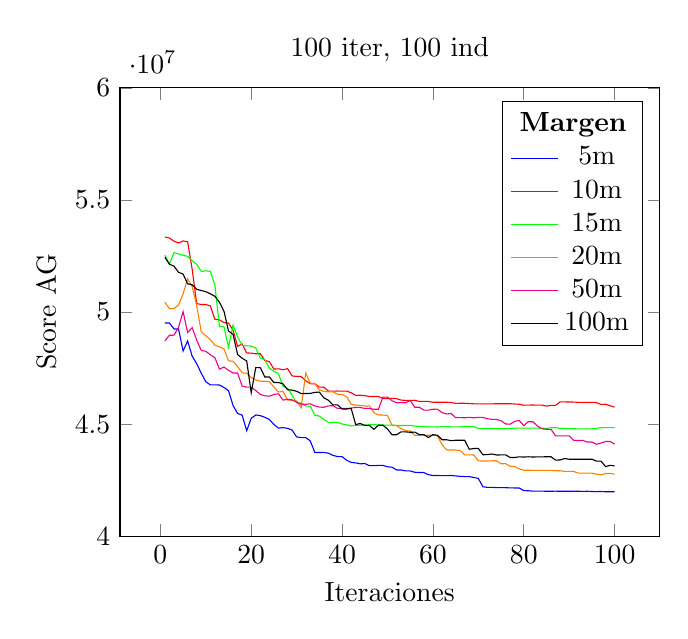
\begin{tikzpicture}
      \begin{axis}[
      title={100 iter, 100 ind},
      xlabel={Iteraciones},
      ylabel={Score AG},
      ymin=40000000,ymax=60000000,
      legend pos=north east]
      
      \addlegendimage{empty legend}
      
      \addplot[color=blue] coordinates {(1,49511238)(2,49511238)(3,49243804)(4,49243804)(5,48261231)(6,48710469)(7,48030981)(8,47694104)(9,47273222)(10,46890093)(11,46748440)(12,46750645)(13,46744881)(14,46638565)(15,46490811)(16,45831135)(17,45476237)(18,45401630)(19,44706526)(20,45258174)(21,45409314)(22,45377674)(23,45303450)(24,45207942)(25,44981775)(26,44819389)(27,44842417)(28,44810410)(29,44735911)(30,44428886)(31,44399896)(32,44399896)(33,44249452)(34,43733996)(35,43733996)(36,43734157)(37,43705707)(38,43602788)(39,43553159)(40,43550659)(41,43390326)(42,43290989)(43,43271696)(44,43227907)(45,43241863)(46,43146253)(47,43146253)(48,43158112)(49,43159311)(50,43096433)(51,43077635)(52,42953636)(53,42953660)(54,42911774)(55,42911783)(56,42851513)(57,42840727)(58,42838872)(59,42743950)(60,42706675)(61,42706597)(62,42702856)(63,42702856)(64,42708500)(65,42688558)(66,42671165)(67,42658165)(68,42658165)(69,42618731)(70,42578313)(71,42205802)(72,42177355)(73,42177727)(74,42168220)(75,42164972)(76,42164972)(77,42155336)(78,42151888)(79,42149914)(80,42033246)(81,42027831)(82,42010212)(83,42009502)(84,42009281)(85,42005841)(86,42006274)(87,42008263)(88,42003674)(89,42004016)(90,42004016)(91,42007774)(92,42006221)(93,41998687)(94,42004115)(95,41992532)(96,41989703)(97,41993451)(98,41982166)(99,41984784)(100,41984813)};
      
      \addplot[color=red] coordinates {(1,53348495)(2,53301783)(3,53157702)(4,53082379)(5,53171982)(6,53136416)(7,51906086)(8,50378497)(9,50335615)(10,50335615)(11,50273504)(12,49671755)(13,49650728)(14,49528002)(15,49508874)(16,49189614)(17,48466702)(18,48576763)(19,48176326)(20,48167324)(21,48137623)(22,48137623)(23,47842380)(24,47786215)(25,47455301)(26,47466827)(27,47428346)(28,47473326)(29,47149856)(30,47127363)(31,47123603)(32,46934615)(33,46804212)(34,46794725)(35,46651293)(36,46645777)(37,46474255)(38,46473111)(39,46475336)(40,46472195)(41,46472017)(42,46403569)(43,46282077)(44,46287675)(45,46270302)(46,46235706)(47,46231842)(48,46231842)(49,46142349)(50,46139697)(51,46146434)(52,46135996)(53,46069692)(54,46059508)(55,46059519)(56,46062768)(57,46012549)(58,46013203)(59,46011258)(60,45976074)(61,45973696)(62,45973430)(63,45976479)(64,45961728)(65,45927913)(66,45928629)(67,45928629)(68,45917695)(69,45904552)(70,45900786)(71,45900786)(72,45900315)(73,45902678)(74,45909732)(75,45909885)(76,45910054)(77,45910054)(78,45896337)(79,45886388)(80,45843712)(81,45847521)(82,45852914)(83,45846220)(84,45846239)(85,45802160)(86,45837177)(87,45837177)(88,45990011)(89,45990471)(90,45985860)(91,45983845)(92,45969874)(93,45969874)(94,45969874)(95,45971055)(96,45962039)(97,45872802)(98,45887511)(99,45819626)(100,45756623)};
      
      \addplot[color=green] coordinates {(1,52540188)(2,52130594)(3,52651126)(4,52589491)(5,52537315)(6,52481524)(7,52282430)(8,52133382)(9,51810769)(10,51840036)(11,51813547)(12,51196913)(13,49356186)(14,49341908)(15,48425998)(16,49420370)(17,48895565)(18,48512514)(19,48495188)(20,48481514)(21,48392672)(22,47950630)(23,47880743)(24,47491130)(25,47361299)(26,47247520)(27,46692084)(28,46593793)(29,46296453)(30,45942250)(31,45942250)(32,45804895)(33,45804895)(34,45400099)(35,45357639)(36,45201572)(37,45075781)(38,45075612)(39,45076069)(40,45007171)(41,44971728)(42,44912943)(43,44948230)(44,44948230)(45,44958629)(46,44972913)(47,44975196)(48,44965822)(49,44959470)(50,44954411)(51,44954411)(52,44944204)(53,44935904)(54,44944365)(55,44943719)(56,44910789)(57,44896328)(58,44894062)(59,44874392)(60,44879807)(61,44871532)(62,44886782)(63,44886440)(64,44878015)(65,44880018)(66,44877448)(67,44891851)(68,44892119)(69,44892189)(70,44808420)(71,44798504)(72,44798525)(73,44798167)(74,44800410)(75,44800410)(76,44796941)(77,44797913)(78,44818641)(79,44818899)(80,44818952)(81,44819264)(82,44818646)(83,44818649)(84,44817114)(85,44810504)(86,44837236)(87,44843850)(88,44813989)(89,44807758)(90,44796324)(91,44797172)(92,44784977)(93,44787259)(94,44783937)(95,44791415)(96,44807762)(97,44844093)(98,44844878)(99,44844117)(100,44844112)};
      
      \addplot[color=orange] coordinates {(1,50435877)(2,50145352)(3,50157397)(4,50313057)(5,50811086)(6,51480972)(7,51135074)(8,50281986)(9,49113503)(10,48940476)(11,48769901)(12,48518423)(13,48446892)(14,48357173)(15,47821212)(16,47809257)(17,47566622)(18,47288834)(19,47268105)(20,47076652)(21,46976287)(22,46909004)(23,46915849)(24,46897161)(25,46652145)(26,46432086)(27,46461550)(28,46071229)(29,46063392)(30,46032626)(31,45723700)(32,47277127)(33,46825792)(34,46815486)(35,46517071)(36,46459334)(37,46443420)(38,46442769)(39,46331549)(40,46327305)(41,46222492)(42,45880192)(43,45849984)(44,45834330)(45,45809563)(46,45811070)(47,45504554)(48,45409698)(49,45405180)(50,45386223)(51,44945517)(52,44934841)(53,44793747)(54,44708529)(55,44693366)(56,44495611)(57,44495611)(58,44505268)(59,44505268)(60,44505268)(61,44470757)(62,44090926)(63,43848683)(64,43843862)(65,43844107)(66,43820983)(67,43624991)(68,43627217)(69,43623199)(70,43362896)(71,43352864)(72,43353789)(73,43364273)(74,43364288)(75,43232103)(76,43235572)(77,43117941)(78,43117139)(79,43003643)(80,42940216)(81,42940216)(82,42938088)(83,42938775)(84,42938775)(85,42938775)(86,42937770)(87,42919709)(88,42919709)(89,42889586)(90,42889017)(91,42889017)(92,42811362)(93,42811362)(94,42811362)(95,42811362)(96,42770437)(97,42729822)(98,42798083)(99,42800440)(100,42766500)};
      
      \addplot[color=magenta] coordinates {(1,48717329)(2,48966210)(3,48966921)(4,49319156)(5,50019140)(6,49085228)(7,49300548)(8,48748851)(9,48283579)(10,48249737)(11,48094051)(12,47964572)(13,47451493)(14,47545834)(15,47403366)(16,47282022)(17,47278768)(18,46696073)(19,46649884)(20,46649884)(21,46497273)(22,46324399)(23,46264488)(24,46244106)(25,46322831)(26,46350483)(27,46069972)(28,46109313)(29,46082458)(30,45977964)(31,45887316)(32,45882240)(33,45907272)(34,45811251)(35,45759020)(36,45750825)(37,45812911)(38,45822042)(39,45699331)(40,45699331)(41,45698098)(42,45713415)(43,45751709)(44,45741926)(45,45699057)(46,45700313)(47,45661434)(48,45661434)(49,46206636)(50,46206659)(51,46040380)(52,45954560)(53,45956260)(54,45950910)(55,46056949)(56,45752285)(57,45752673)(58,45624208)(59,45623072)(60,45662806)(61,45667781)(62,45515516)(63,45452361)(64,45474217)(65,45289479)(66,45292544)(67,45281310)(68,45300666)(69,45280532)(70,45301998)(71,45301998)(72,45239118)(73,45212147)(74,45208027)(75,45149685)(76,45007640)(77,44996105)(78,45125894)(79,45161064)(80,44931078)(81,45108037)(82,45107152)(83,44918290)(84,44789198)(85,44769058)(86,44765192)(87,44473953)(88,44473953)(89,44474286)(90,44475874)(91,44274491)(92,44269511)(93,44271867)(94,44203240)(95,44204556)(96,44098704)(97,44157947)(98,44223960)(99,44225568)(100,44107082)};
      
      \addplot[color=black] coordinates {(1,52443460)(2,52131682)(3,52048584)(4,51771908)(5,51695366)(6,51258589)(7,51215128)(8,51015774)(9,50958275)(10,50908911)(11,50810487)(12,50703392)(13,50435979)(14,50036864)(15,49154142)(16,49003800)(17,48104633)(18,47938516)(19,47820077)(20,46397886)(21,47523229)(22,47516701)(23,47101433)(24,47100645)(25,46854973)(26,46855132)(27,46796446)(28,46536340)(29,46516691)(30,46464010)(31,46361621)(32,46365311)(33,46369206)(34,46416221)(35,46426871)(36,46170322)(37,46061798)(38,45856459)(39,45860386)(40,45674601)(41,45674601)(42,45702406)(43,44978224)(44,45026591)(45,44941568)(46,44941628)(47,44767492)(48,44949843)(49,44950214)(50,44780704)(51,44526300)(52,44526300)(53,44655285)(54,44653901)(55,44634543)(56,44642582)(57,44531820)(58,44531820)(59,44402500)(60,44528866)(61,44501699)(62,44303744)(63,44303744)(64,44261664)(65,44279509)(66,44279509)(67,44279509)(68,43879363)(69,43912626)(70,43915204)(71,43631815)(72,43642401)(73,43666652)(74,43622722)(75,43625469)(76,43629748)(77,43509552)(78,43512242)(79,43541351)(80,43529914)(81,43542851)(82,43531224)(83,43539085)(84,43539122)(85,43544744)(86,43545505)(87,43394209)(88,43400456)(89,43463580)(90,43432512)(91,43432699)(92,43433077)(93,43433077)(94,43433077)(95,43435006)(96,43349193)(97,43349193)(98,43108046)(99,43160325)(100,43138326)};
      
        \addlegendentry{\hspace{-.6cm}\textbf{Margen}}
        \addlegendentry{5m}
        \addlegendentry{10m}
        \addlegendentry{15m}
        \addlegendentry{20m}
        \addlegendentry{50m}
        \addlegendentry{100m}
      \end{axis}
    \end{tikzpicture}
    \caption{Ejecuciones con diferentes márgenes}
    \label{fig:adv_multi_margin}
\end{figure}

A partir de los resultados visibles en la figura \ref{fig:adv_multi_margin} se puede observar como, por regla general, el impacto obtenido al cambiar el valor de margen a utilizar entre puntos no es muy significativo. Para la mayoría de los valores utilizados, la media entre las diferentes ejecuciones se mueve en general entre los mismos valores de \textit{fitness} conforme avanzan las iteraciones. Entre los diferentes márgenes, el único de ellos que destaca (de forma positiva) es de 5 metros, con el cual se obtiene, de forma visible una puntuación mejor que con el resto de las opciones de los márgenes. Este hecho tiene sentido, basándose en que, de cara a un cálculo más preciso, este margen de 5 metros permite eliminar posibles errores obtenidos de la ruta original (con algunos puntos solapados, o muy cercanos) mientras que el cálculo por cada uno de los \textit{chunks} es más acotado a un tramo de vía de verdad.

\begin{table}[h]
    \centering
    \begin{tabular}{l*6c}
    \toprule
    \backslashbox{\textbf{Medida}}{\textbf{Margen}} & \textbf{5m} & \textbf{10m} & \textbf{15m} & \textbf{20m} & \textbf{50m} & \textbf{100m} \\
    \midrule
    \textbf{Desviación típica} & 2174289 & 2101684 & 2476409 & 2637240 & 1579917 & 2474392 \\
    \textbf{Media} & 44667300 & 46763000 & 46294552 & 45511247 & 45688738 & 45718853 \\
    \textbf{Coef. de variación} & 4,87\% & 4,49\% & 5,35\% & 5,81\% & 3,46\% & 5,41\% \\
    \bottomrule
    \end{tabular}
    \caption{Valores de dispersión según márgenes (100 ind.)}
    \label{tab:adv_margin}
\end{table}

Al igual que con las pruebas ya realizadas, se ha reunido en la tabla \ref{tab:adv_margin} la misma información estadística de las diferentes series con distintos márgenes. Con estos datos, se puede verificar, a través de la media obtenida al utilizar el margen de 5 metros, que a través de dicho margen se obtienen unos resultados con un consumo menor al resto. En este caso, al tratarse del mismo modelo y grupo de individuos durante todas las ejecuciones, valores como la desviación típica, y, sobre todo, el coeficiente de variación, no se ven tan alterados como en pruebas anteriores, siendo su rango de valores (en el caso del coeficiente de variación) de un 2\%.\newline

\textbf{Método alternativo de corrección de individuos}\newline
Otra de las pruebas realizadas se ha tratado de la modificación del procedimiento para corregir a aquellos individuos que se detectan como no válidos durante la ejecución para el modelo, es decir, aquellos en los que, en alguno de sus \textit{chunks}, alguna de las  condiciones indicadas en el capítulo \ref{section:adv_gen_alg} no se cumplen.

Es importante destacar en este punto la segunda condición, que establece que, a partir de cierto punto, el vehículo debe de llevar una velocidad mínima. Esto se debe al hecho que, cuando la métrica de optimización se basa únicamente en consumos eléctricos, algunas ejecuciones tienden a devolver resultados donde la velocidad alcanzada por un vehículo es mínima, y, por lo tanto, su consumo menor.

En cuanto a la técnica de corrección aplicada, esta consiste en los siguientes cambios: en el procedimiento de cálculo del valor de \textit{fitness} de cada uno de los individuos, se comprueba, para cada uno de ellos la validez del individuo, devolviendo, como ya se ha podido ver anteriormente (sobre todo en el modelo básico), un valor de $-1$ en el caso en el que no sea válido. Es en este punto, una vez obtenida la puntuación de todos los individuos, donde, para aquellos que tienen esta puntuación especial, se pasa a aplicar la corrección.

Una vez ya detectado un individuo ``defectuoso``, se recorren los \textit{chunks} que lo conforman buscando aquellos que hacen incumplir las condiciones de correctitud. Es importante indicar como, durante las pruebas, en la amplia mayoría de los casos, cuando un individuo no es correcto, el problema se suele observar en un grupo contiguo de \textit{chunks}, en lugar de puntos aislados. Es por ello, que la corrección no se debe centrar en un primer punto de fallo, si no en el individuo entero.

\begin{figure}[!htb]
    \centering
    \includegraphics[width=0.5\textwidth]{AG_Repair.png}
    \caption{Diagrama de reparación de un individuo}
    \label{fig:adv_repair_diagram}
\end{figure}

Cuando un \textit{chunk} inválido ya ha sido detectado, el primer paso que se realiza para intentar corregirlo se basa en realizar un suavizado de la aceleración a realizar, multiplicando el valor que tenía originalmente por un factor de 0,9 si se debe a un exceso de velocidad, o por un factor de 1,1 si es por falta de velocidad. En este punto, se vuelve a comprobar si el problema local (del \textit{chunk}) se ha corregido. En dicho caso, si esta corrección consigue arreglar al individuo se termina el proceso de corrección; y, en el caso contrario, se procede a continuar con el mismo proceso ya descrito en los siguientes \textit{chunks} que conforman al individuo.

\begin{figure}[!htb]
    \centering
    % Figura 20
    \begin{subfigure}[b]{0.44\textwidth}
        \resizebox{\linewidth}{!}{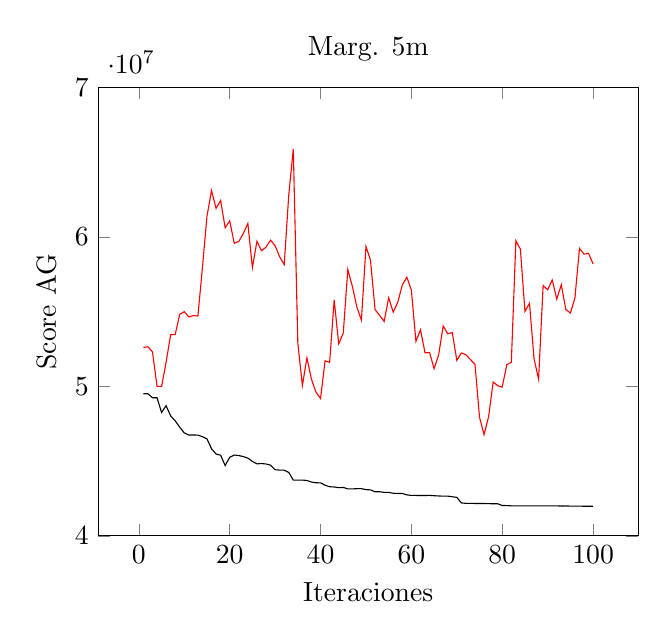
\begin{tikzpicture}
            \begin{axis}[
              title={Marg. 5m},
              xlabel={Iteraciones},
              ylabel={Score AG},
              ymin=40000000,ymax=70000000]
              
              \addplot[color=red] coordinates {(1,52608990)(2,52652841)(3,52313151)(4,50016487)(5,49983444)(6,51622143)(7,53466368)(8,53471966)(9,54829460)(10,55002570)(11,54650560)(12,54743609)(13,54709456)(14,57968265)(15,61390899)(16,63106326)(17,61918949)(18,62440156)(19,60622837)(20,61077639)(21,59583871)(22,59698009)(23,60240323)(24,60904701)(25,57957547)(26,59716318)(27,59081948)(28,59323667)(29,59788103)(30,59415984)(31,58666948)(32,58152196)(33,62794760)(34,65883503)(35,52890253)(36,50061395)(37,51909290)(38,50472807)(39,49615900)(40,49192770)(41,51718905)(42,51610388)(43,55785894)(44,52854812)(45,53567768)(46,57818358)(47,56703924)(48,55309511)(49,54433204)(50,59368027)(51,58436195)(52,55141205)(53,54765867)(54,54350971)(55,55931047)(56,54973258)(57,55636051)(58,56794665)(59,57316257)(60,56427515)(61,53020385)(62,53789581)(63,52248644)(64,52265788)(65,51191657)(66,52108782)(67,54047982)(68,53522867)(69,53605362)(70,51746265)(71,52241442)(72,52124675)(73,51793898)(74,51482484)(75,47933314)(76,46773934)(77,47984713)(78,50298973)(79,50046792)(80,49958206)(81,51459289)(82,51614447)(83,59755949)(84,59179930)(85,55023650)(86,55562216)(87,51857910)(88,50484656)(89,56753133)(90,56466813)(91,57126584)(92,55850323)(93,56804542)(94,55154980)(95,54908903)(96,55916315)(97,59240655)(98,58850680)(99,58904655)(100,58191812)};
              
              \addplot[color=black] coordinates {(1,49511238)(2,49511238)(3,49243804)(4,49243804)(5,48261231)(6,48710469)(7,48030981)(8,47694104)(9,47273222)(10,46890093)(11,46748440)(12,46750645)(13,46744881)(14,46638565)(15,46490811)(16,45831135)(17,45476237)(18,45401630)(19,44706526)(20,45258174)(21,45409314)(22,45377674)(23,45303450)(24,45207942)(25,44981775)(26,44819389)(27,44842417)(28,44810410)(29,44735911)(30,44428886)(31,44399896)(32,44399896)(33,44249452)(34,43733996)(35,43733996)(36,43734157)(37,43705707)(38,43602788)(39,43553159)(40,43550659)(41,43390326)(42,43290989)(43,43271696)(44,43227907)(45,43241863)(46,43146253)(47,43146253)(48,43158112)(49,43159311)(50,43096433)(51,43077635)(52,42953636)(53,42953660)(54,42911774)(55,42911783)(56,42851513)(57,42840727)(58,42838872)(59,42743950)(60,42706675)(61,42706597)(62,42702856)(63,42702856)(64,42708500)(65,42688558)(66,42671165)(67,42658165)(68,42658165)(69,42618731)(70,42578313)(71,42205802)(72,42177355)(73,42177727)(74,42168220)(75,42164972)(76,42164972)(77,42155336)(78,42151888)(79,42149914)(80,42033246)(81,42027831)(82,42010212)(83,42009502)(84,42009281)(85,42005841)(86,42006274)(87,42008263)(88,42003674)(89,42004016)(90,42004016)(91,42007774)(92,42006221)(93,41998687)(94,42004115)(95,41992532)(96,41989703)(97,41993451)(98,41982166)(99,41984784)(100,41984813)};
            \end{axis}
        \end{tikzpicture}}
    \end{subfigure}
    % Figura 21
    \begin{subfigure}[b]{0.44\textwidth}
        \resizebox{\linewidth}{!}{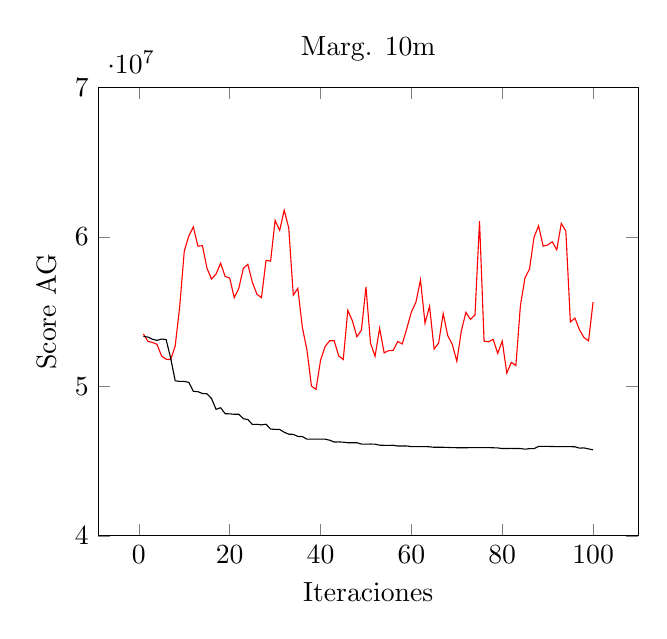
\begin{tikzpicture}
            \begin{axis}[
              title={Marg. 10m},
              xlabel={Iteraciones},
              ylabel={Score AG},
              ymin=40000000,ymax=70000000]
              
              \addplot[color=red] coordinates {(1,53512750)(2,53015975)(3,52944982)(4,52817681)(5,52036146)(6,51823144)(7,51793523)(8,52702732)(9,55361076)(10,59057535)(11,60073659)(12,60670419)(13,59392020)(14,59415443)(15,57903460)(16,57192089)(17,57524007)(18,58244238)(19,57362104)(20,57255767)(21,55939698)(22,56560877)(23,57903776)(24,58171799)(25,56953722)(26,56171562)(27,55938138)(28,58443489)(29,58383329)(30,61112897)(31,60444817)(32,61797393)(33,60590409)(34,56112047)(35,56561224)(36,53947431)(37,52448256)(38,50022703)(39,49806522)(40,51750099)(41,52672151)(42,53055052)(43,53057109)(44,52044716)(45,51800218)(46,55090590)(47,54404141)(48,53324824)(49,53768339)(50,56657865)(51,52895256)(52,52017340)(53,53890362)(54,52247363)(55,52393687)(56,52415699)(57,53006377)(58,52843556)(59,53889145)(60,54987264)(61,55637744)(62,57130968)(63,54227147)(64,55363817)(65,52503632)(66,52910139)(67,54879967)(68,53396381)(69,52819535)(70,51684088)(71,53719658)(72,54959956)(73,54483804)(74,54782355)(75,61064413)(76,53026329)(77,52988548)(78,53151649)(79,52215146)(80,53034437)(81,50895005)(82,51612298)(83,51396403)(84,55405364)(85,57267985)(86,57851153)(87,59989792)(88,60747855)(89,59391108)(90,59465369)(91,59680066)(92,59144873)(93,60905932)(94,60401119)(95,54309632)(96,54573125)(97,53793211)(98,53271855)(99,53054325)(100,55645448)};
              
              \addplot[color=black] coordinates {(1,53348495)(2,53301783)(3,53157702)(4,53082379)(5,53171982)(6,53136416)(7,51906086)(8,50378497)(9,50335615)(10,50335615)(11,50273504)(12,49671755)(13,49650728)(14,49528002)(15,49508874)(16,49189614)(17,48466702)(18,48576763)(19,48176326)(20,48167324)(21,48137623)(22,48137623)(23,47842380)(24,47786215)(25,47455301)(26,47466827)(27,47428346)(28,47473326)(29,47149856)(30,47127363)(31,47123603)(32,46934615)(33,46804212)(34,46794725)(35,46651293)(36,46645777)(37,46474255)(38,46473111)(39,46475336)(40,46472195)(41,46472017)(42,46403569)(43,46282077)(44,46287675)(45,46270302)(46,46235706)(47,46231842)(48,46231842)(49,46142349)(50,46139697)(51,46146434)(52,46135996)(53,46069692)(54,46059508)(55,46059519)(56,46062768)(57,46012549)(58,46013203)(59,46011258)(60,45976074)(61,45973696)(62,45973430)(63,45976479)(64,45961728)(65,45927913)(66,45928629)(67,45928629)(68,45917695)(69,45904552)(70,45900786)(71,45900786)(72,45900315)(73,45902678)(74,45909732)(75,45909885)(76,45910054)(77,45910054)(78,45896337)(79,45886388)(80,45843712)(81,45847521)(82,45852914)(83,45846220)(84,45846239)(85,45802160)(86,45837177)(87,45837177)(88,45990011)(89,45990471)(90,45985860)(91,45983845)(92,45969874)(93,45969874)(94,45969874)(95,45971055)(96,45962039)(97,45872802)(98,45887511)(99,45819626)(100,45756623)};
            \end{axis}
        \end{tikzpicture}}
    \end{subfigure}
    \newline
    % Figura 22
    \begin{subfigure}[b]{0.44\textwidth}
        \resizebox{\linewidth}{!}{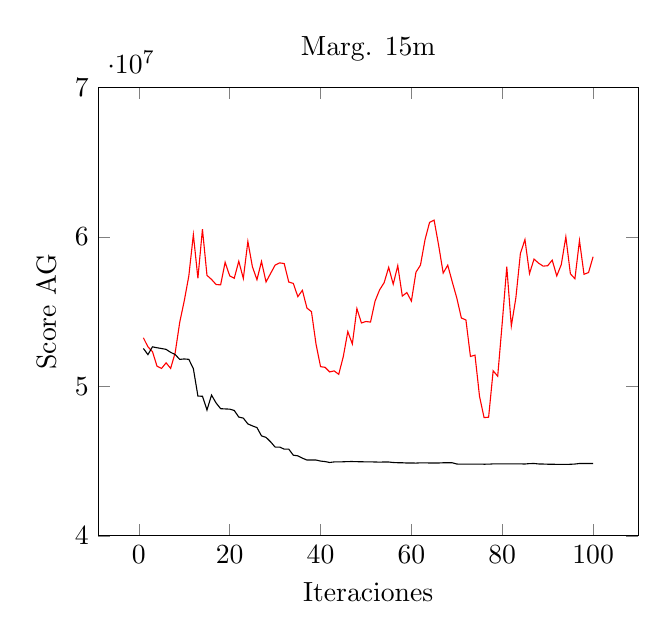
\begin{tikzpicture}
            \begin{axis}[
              title={Marg. 15m},
              xlabel={Iteraciones},
              ylabel={Score AG},
              ymin=40000000,ymax=70000000]
              
              \addplot[color=red] coordinates {(1,53255648)(2,52649692)(3,52330434)(4,51352390)(5,51208115)(6,51579001)(7,51208562)(8,52258805)(9,54297071)(10,55734614)(11,57395033)(12,60156471)(13,57241019)(14,60521727)(15,57432654)(16,57161265)(17,56822760)(18,56796222)(19,58311480)(20,57400859)(21,57239643)(22,58377011)(23,57225840)(24,59700786)(25,58008162)(26,57143960)(27,58359548)(28,56991731)(29,57560745)(30,58119613)(31,58270083)(32,58223439)(33,56988459)(34,56895379)(35,56009406)(36,56433954)(37,55246368)(38,55005415)(39,52840810)(40,51324059)(41,51279842)(42,50972497)(43,51039758)(44,50809928)(45,51988455)(46,53672693)(47,52842203)(48,55210458)(49,54248168)(50,54345349)(51,54306654)(52,55706706)(53,56462017)(54,56944742)(55,57970760)(56,56840998)(57,58081536)(58,56046876)(59,56282961)(60,55711497)(61,57640321)(62,58122508)(63,59820314)(64,60980224)(65,61127853)(66,59441745)(67,57585927)(68,58114808)(69,56991101)(70,55909965)(71,54578721)(72,54452022)(73,52005772)(74,52093172)(75,49333318)(76,47913263)(77,47942902)(78,51046191)(79,50685576)(80,54267996)(81,58008979)(82,54042619)(83,55928630)(84,58908841)(85,59827061)(86,57555624)(87,58521350)(88,58249930)(89,58050497)(90,58079244)(91,58451140)(92,57398915)(93,58158148)(94,60011224)(95,57539176)(96,57207408)(97,59763375)(98,57505564)(99,57622396)(100,58681312)};
              
              \addplot[color=black] coordinates {(1,52540188)(2,52130594)(3,52651126)(4,52589491)(5,52537315)(6,52481524)(7,52282430)(8,52133382)(9,51810769)(10,51840036)(11,51813547)(12,51196913)(13,49356186)(14,49341908)(15,48425998)(16,49420370)(17,48895565)(18,48512514)(19,48495188)(20,48481514)(21,48392672)(22,47950630)(23,47880743)(24,47491130)(25,47361299)(26,47247520)(27,46692084)(28,46593793)(29,46296453)(30,45942250)(31,45942250)(32,45804895)(33,45804895)(34,45400099)(35,45357639)(36,45201572)(37,45075781)(38,45075612)(39,45076069)(40,45007171)(41,44971728)(42,44912943)(43,44948230)(44,44948230)(45,44958629)(46,44972913)(47,44975196)(48,44965822)(49,44959470)(50,44954411)(51,44954411)(52,44944204)(53,44935904)(54,44944365)(55,44943719)(56,44910789)(57,44896328)(58,44894062)(59,44874392)(60,44879807)(61,44871532)(62,44886782)(63,44886440)(64,44878015)(65,44880018)(66,44877448)(67,44891851)(68,44892119)(69,44892189)(70,44808420)(71,44798504)(72,44798525)(73,44798167)(74,44800410)(75,44800410)(76,44796941)(77,44797913)(78,44818641)(79,44818899)(80,44818952)(81,44819264)(82,44818646)(83,44818649)(84,44817114)(85,44810504)(86,44837236)(87,44843850)(88,44813989)(89,44807758)(90,44796324)(91,44797172)(92,44784977)(93,44787259)(94,44783937)(95,44791415)(96,44807762)(97,44844093)(98,44844878)(99,44844117)(100,44844112)};
            \end{axis}
        \end{tikzpicture}}
    \end{subfigure}
    % FIGURE 22
    \begin{subfigure}[b]{0.44\textwidth}
        \resizebox{\linewidth}{!}{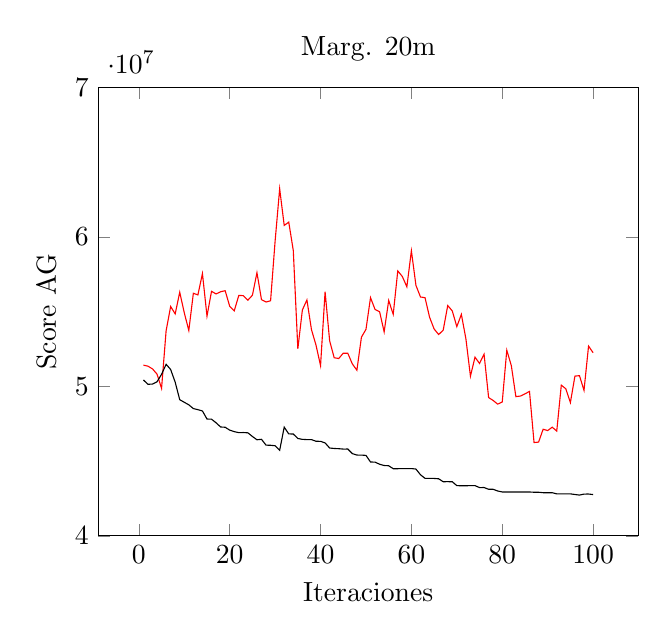
\begin{tikzpicture}
            \begin{axis}[
              title={Marg. 20m},
              xlabel={Iteraciones},
              ylabel={Score AG},
              ymin=40000000,ymax=70000000]
              
              \addplot[color=red] coordinates {(1,51425358)(2,51357313)(3,51175292)(4,50826084)(5,49869943)(6,53723341)(7,55349260)(8,54855249)(9,56304903)(10,54929490)(11,53743189)(12,56235924)(13,56125896)(14,57554984)(15,54705957)(16,56365736)(17,56190830)(18,56336531)(19,56406846)(20,55365771)(21,55059563)(22,56089257)(23,56077500)(24,55772710)(25,56102403)(26,57613129)(27,55810643)(28,55649947)(29,55733803)(30,59735653)(31,63227528)(32,60773840)(33,60997544)(34,59094929)(35,52515896)(36,55119813)(37,55788287)(38,53803809)(39,52765172)(40,51392357)(41,56339641)(42,53057883)(43,51921735)(44,51868614)(45,52225575)(46,52219139)(47,51507594)(48,51085569)(49,53295382)(50,53821030)(51,55940249)(52,55149495)(53,55000922)(54,53652353)(55,55751200)(56,54829656)(57,57730244)(58,57359768)(59,56667746)(60,59078923)(61,56762767)(62,55986334)(63,55939064)(64,54634355)(65,53845210)(66,53475413)(67,53764481)(68,55415237)(69,55053346)(70,54003953)(71,54820744)(72,53187783)(73,50684911)(74,51960194)(75,51539276)(76,52153692)(77,49257165)(78,49060506)(79,48816648)(80,48963034)(81,52424110)(82,51390654)(83,49316867)(84,49357641)(85,49503306)(86,49667959)(87,46246289)(88,46275108)(89,47135603)(90,47048426)(91,47273047)(92,47012540)(93,50083971)(94,49843130)(95,48918057)(96,50692164)(97,50722358)(98,49736423)(99,52700616)(100,52256738)};
              
              \addplot[color=black] coordinates {(1,50435877)(2,50145352)(3,50157397)(4,50313057)(5,50811086)(6,51480972)(7,51135074)(8,50281986)(9,49113503)(10,48940476)(11,48769901)(12,48518423)(13,48446892)(14,48357173)(15,47821212)(16,47809257)(17,47566622)(18,47288834)(19,47268105)(20,47076652)(21,46976287)(22,46909004)(23,46915849)(24,46897161)(25,46652145)(26,46432086)(27,46461550)(28,46071229)(29,46063392)(30,46032626)(31,45723700)(32,47277127)(33,46825792)(34,46815486)(35,46517071)(36,46459334)(37,46443420)(38,46442769)(39,46331549)(40,46327305)(41,46222492)(42,45880192)(43,45849984)(44,45834330)(45,45809563)(46,45811070)(47,45504554)(48,45409698)(49,45405180)(50,45386223)(51,44945517)(52,44934841)(53,44793747)(54,44708529)(55,44693366)(56,44495611)(57,44495611)(58,44505268)(59,44505268)(60,44505268)(61,44470757)(62,44090926)(63,43848683)(64,43843862)(65,43844107)(66,43820983)(67,43624991)(68,43627217)(69,43623199)(70,43362896)(71,43352864)(72,43353789)(73,43364273)(74,43364288)(75,43232103)(76,43235572)(77,43117941)(78,43117139)(79,43003643)(80,42940216)(81,42940216)(82,42938088)(83,42938775)(84,42938775)(85,42938775)(86,42937770)(87,42919709)(88,42919709)(89,42889586)(90,42889017)(91,42889017)(92,42811362)(93,42811362)(94,42811362)(95,42811362)(96,42770437)(97,42729822)(98,42798083)(99,42800440)(100,42766500)};
            \end{axis}
        \end{tikzpicture}}
    \end{subfigure}
    \newline
    % FIGURE 23
    \begin{subfigure}[b]{0.44\textwidth}
        \resizebox{\linewidth}{!}{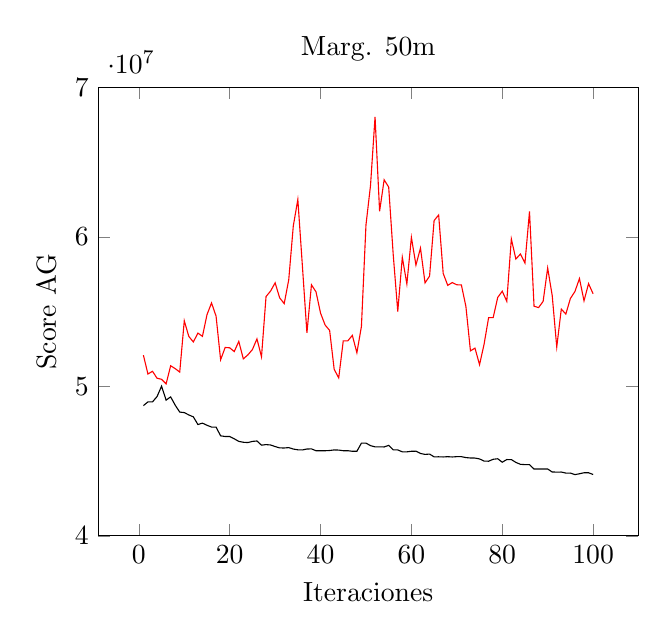
\begin{tikzpicture}
            \begin{axis}[
              title={Marg. 50m},
              xlabel={Iteraciones},
              ylabel={Score AG},
              ymin=40000000,ymax=70000000]
              
              \addplot[color=red] coordinates {(1,52093476)(2,50830539)(3,51014262)(4,50552019)(5,50477128)(6,50172755)(7,51385066)(8,51191802)(9,50963370)(10,54392808)(11,53344627)(12,52979338)(13,53569282)(14,53353873)(15,54800636)(16,55586979)(17,54704472)(18,51784282)(19,52608464)(20,52585979)(21,52333672)(22,53011764)(23,51845117)(24,52110346)(25,52469268)(26,53183076)(27,51985369)(28,56016174)(29,56383222)(30,56933757)(31,55926907)(32,55545433)(33,57142876)(34,60736846)(35,62512340)(36,58080656)(37,53579888)(38,56801632)(39,56328318)(40,54907966)(41,54112141)(42,53747631)(43,51148677)(44,50570629)(45,53052449)(46,53052910)(47,53416342)(48,52254463)(49,54018648)(50,60807594)(51,63449842)(52,68042119)(53,61719692)(54,63827171)(55,63343485)(56,58812347)(57,55012928)(58,58642589)(59,56855152)(60,59973398)(61,58122538)(62,59259586)(63,56930272)(64,57380792)(65,61101213)(66,61474450)(67,57562778)(68,56764484)(69,56952431)(70,56803144)(71,56794110)(72,55349990)(73,52381612)(74,52563161)(75,51456782)(76,52824822)(77,54606791)(78,54603564)(79,55951938)(80,56375343)(81,55696716)(82,59872700)(83,58524081)(84,58861318)(85,58254102)(86,61706585)(87,55367969)(88,55276639)(89,55693606)(90,57927650)(91,56077426)(92,52638652)(93,55177012)(94,54843115)(95,55884374)(96,56352862)(97,57219829)(98,55726491)(99,56878922)(100,56201149)};
              
              \addplot[color=black] coordinates {(1,48717329)(2,48966210)(3,48966921)(4,49319156)(5,50019140)(6,49085228)(7,49300548)(8,48748851)(9,48283579)(10,48249737)(11,48094051)(12,47964572)(13,47451493)(14,47545834)(15,47403366)(16,47282022)(17,47278768)(18,46696073)(19,46649884)(20,46649884)(21,46497273)(22,46324399)(23,46264488)(24,46244106)(25,46322831)(26,46350483)(27,46069972)(28,46109313)(29,46082458)(30,45977964)(31,45887316)(32,45882240)(33,45907272)(34,45811251)(35,45759020)(36,45750825)(37,45812911)(38,45822042)(39,45699331)(40,45699331)(41,45698098)(42,45713415)(43,45751709)(44,45741926)(45,45699057)(46,45700313)(47,45661434)(48,45661434)(49,46206636)(50,46206659)(51,46040380)(52,45954560)(53,45956260)(54,45950910)(55,46056949)(56,45752285)(57,45752673)(58,45624208)(59,45623072)(60,45662806)(61,45667781)(62,45515516)(63,45452361)(64,45474217)(65,45289479)(66,45292544)(67,45281310)(68,45300666)(69,45280532)(70,45301998)(71,45301998)(72,45239118)(73,45212147)(74,45208027)(75,45149685)(76,45007640)(77,44996105)(78,45125894)(79,45161064)(80,44931078)(81,45108037)(82,45107152)(83,44918290)(84,44789198)(85,44769058)(86,44765192)(87,44473953)(88,44473953)(89,44474286)(90,44475874)(91,44274491)(92,44269511)(93,44271867)(94,44203240)(95,44204556)(96,44098704)(97,44157947)(98,44223960)(99,44225568)(100,44107082)};
            \end{axis}
        \end{tikzpicture}}
    \end{subfigure}
    % FIGURE 24
    \begin{subfigure}[b]{0.44\textwidth}
        \resizebox{\linewidth}{!}{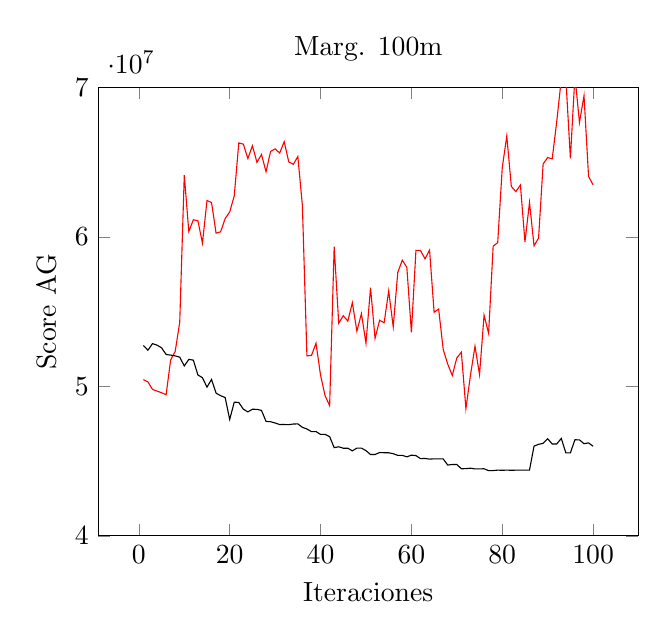
\begin{tikzpicture}
            \begin{axis}[
              title={Marg. 100m},
              xlabel={Iteraciones},
              ylabel={Score AG},
              ymin=40000000,ymax=70000000]
              
              \addplot[color=red] coordinates {(1,50453634)(2,50304132)(3,49803484)(4,49688507)(5,49579801)(6,49445164)(7,51773870)(8,52343887)(9,54296340)(10,64142884)(11,60367160)(12,61152796)(13,61088836)(14,59586996)(15,62436241)(16,62310195)(17,60259353)(18,60345229)(19,61233460)(20,61674643)(21,62749613)(22,66293959)(23,66217142)(24,65252595)(25,66107106)(26,64995658)(27,65523227)(28,64366120)(29,65724387)(30,65896421)(31,65618958)(32,66379042)(33,65028420)(34,64866339)(35,65381338)(36,62123947)(37,52050233)(38,52074641)(39,52887834)(40,50751896)(41,49375272)(42,48712740)(43,59362235)(44,54236081)(45,54732965)(46,54372433)(47,55601388)(48,53700306)(49,54873322)(50,52886478)(51,56613377)(52,53218156)(53,54428681)(54,54261387)(55,56389431)(56,53987118)(57,57629912)(58,58451361)(59,57965529)(60,53618455)(61,59109336)(62,59094851)(63,58538713)(64,59124495)(65,54965120)(66,55180451)(67,52477736)(68,51496126)(69,50732140)(70,51913411)(71,52292470)(72,48515940)(73,50745681)(74,52688774)(75,50794992)(76,54774284)(77,53558811)(78,59388304)(79,59619665)(80,64629364)(81,66754930)(82,63388203)(83,63037271)(84,63482146)(85,59663484)(86,62315341)(87,59407975)(88,59933532)(89,64886943)(90,65318558)(91,65232510)(92,67734791)(93,70564936)(94,70632535)(95,65267256)(96,70770528)(97,67667448)(98,69459872)(99,64054354)(100,63491254)};
              
              \addplot[color=black] coordinates {(1,52739608)(2,52426069)(3,52863490)(4,52765419)(5,52584554)(6,52140265)(7,52096055)(8,52047714)(9,51960646)(10,51371355)(11,51812271)(12,51760648)(13,50765421)(14,50587078)(15,49954287)(16,50468446)(17,49552263)(18,49381147)(19,49257900)(20,47791472)(21,48950615)(22,48925832)(23,48480166)(24,48298286)(25,48472039)(26,48469248)(27,48394707)(28,47660397)(29,47640273)(30,47553991)(31,47449201)(32,47452977)(33,47440982)(34,47484490)(35,47495384)(36,47264975)(37,47153878)(38,46976150)(39,46980173)(40,46789852)(41,46790404)(42,46644205)(43,45905099)(44,45962012)(45,45867687)(46,45867687)(47,45689960)(48,45876068)(49,45876445)(50,45703441)(51,45446054)(52,45446054)(53,45577704)(54,45565202)(55,45561319)(56,45500523)(57,45387632)(58,45387632)(59,45290256)(60,45401559)(61,45373696)(62,45171862)(63,45180813)(64,45137900)(65,45154787)(66,45154787)(67,45148474)(68,44740476)(69,44777040)(70,44779669)(71,44490701)(72,44501809)(73,44527848)(74,44483364)(75,44486130)(76,44490493)(77,44367927)(78,44370727)(79,44400411)(80,44388747)(81,44401950)(82,44390093)(83,44398109)(84,44398147)(85,44403880)(86,44404658)(87,46007396)(88,46126120)(89,46193208)(90,46500075)(91,46151480)(92,46151881)(93,46523118)(94,45554717)(95,45556741)(96,46431470)(97,46426395)(98,46168130)(99,46224698)(100,45998804)};
            \end{axis}
        \end{tikzpicture}}
    \end{subfigure}
    \newline
    % FIGURE 25?
    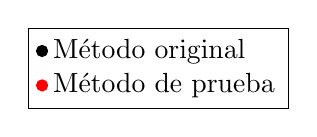
\begin{tikzpicture}
    \begin{customlegend}[legend entries={Método original, Método de prueba}, legend cell align={left}]
    \addlegendimage{black,fill=black!50!black,mark=*,only marks} % sharp plot
    \addlegendimage{red,fill=red!50!red,mark=*,only marks} % sharp plot
    \end{customlegend}
    \end{tikzpicture}
    \caption{Comparaciones entre los métodos de corrección}
    \label{fig:adv_new_method}
\end{figure}

En el caso en el que tras el primer intento de corrección de un \textit{chunk} este sigue sin ser válido, se pasa entonces a realizar un segundo suavizado, basado disminuir o incrementar, según que condición falle, la aceleración (que se encuentra escalada en un rango entre -1 y 1) en escalones de 0.05. Tras esto se comprueba de nuevo si se soluciona el problema. En caso de no solucionarlo, se repite este último proceso tantas veces sean necesarias hasta que el \textit{chunk} es válido. En caso de realizar todos los intentos posibles y no conseguir la corrección del \textit{chunk}, este se deja tal y como estaba en su último intento de corrección para intentar corregirlo en la siguiente iteración de nuevo.

Todo este proceso descrito se puede ver esquematizado en la figura \ref{fig:adv_repair_diagram}, donde el valor $x$ hace referencia al \textit{chunk} que se encuentra en procesamiento y la operación $x=x+1$ se aplica para saltar al siguiente \textit{chunk} de la lista que conforma al individuo.

Finalmente, en la figura \ref{fig:adv_new_method} se pueden observar los resultados obtenidos al comparar este nuevo método con el método de reemplazo utilizado inicialmente. En estas gráficas, ambas series de datos representan, para cada iteración, la media de los valores correspondientes al mejor individuo existente en dicha iteración. Las series en color rojo hacen referencia al nuevo método, mientras que las series en negro se corresponden al método ya probado anteriormente. En la totalidad de las series\footnotemark  ejecutadas es observable como el utilizar este nuevo método propuesto no aporta ningún tipo de mejora. En la mayoría de las combinaciones se puede ver como con este método el algoritmo es incapaz de aprender, y, pese a los valores puntuales, la tendencia de la gráfica en plana. Incluso en algunos casos, se vuelve a vislumbrar los problemas que aparecían con el modelo básico, donde conforme avanzan las iteraciones, la puntuación obtenida va empeorando poco a poco.

Un último hecho a destacar se trata del efecto que tiene el reinicio de las poblaciones en las gráficas. Dado que no hay prácticamente aprendizaje, con 100 iteraciones, este reinicio salta tras 30 iteraciones seguidas estancadas, lo que se corresponde con un primer reinicio entre las iteraciones 30 y 40, muy observable en todas las gráficas, con cambios muy abruptos, y algunos otros reinicios alrededor de las iteraciones 70 y 80, muy visibles por ejemplo en las gráficas de 15 y 100 metros de márgenes.

\footnotetext{Al igual que el resto de las pruebas realizadas, las series han consistido en la ejecución del sistema de forma independiente en 5 ocasiones. Para esta prueba, el número de individuos utilizado ha sido de 100, siguiendo el mejor resultado obtenido en las pruebas anteriores.}

\newpage
\subsection{Métricas basadas en el tiempo}
Una vez analizado el modelo avanzado, centrado en una métrica de optimización basada únicamente en los consumos eléctricos, a continuación, se detallan las pruebas que se han realizado sobre el modelo de optimización utilizando una métrica basada únicamente en el tiempo empleado para realizar una ruta, utilizando el modelo descrito en la sección \ref{section:adv_alt_models}.

Siguiendo los resultados obtenidos con las pruebas anteriores, para esta serie de pruebas se va a utilizar el método original de corrección de individuos, es decir, el reemplazo por uno nuevo, al igual que el reinicio general de la población si no se mejora la mejor puntuación durante una serie de iteraciones. Para estas pruebas, se ha utilizado directamente una población de 100 individuos, ya que es con la que se obtenía mejores resultados en las pruebas anteriores. También, siguiendo el mismo patrón que en las pruebas anteriores, la primera prueba realizada se trata de la comparación del efecto que tiene el número de iteraciones a realizar sobre la puntuación final obtenida.

\begin{figure}[!htb]
% FIGURE 26
\begin{subfigure}[b]{0.43\textwidth}
\centering
\resizebox{\linewidth}{!}{
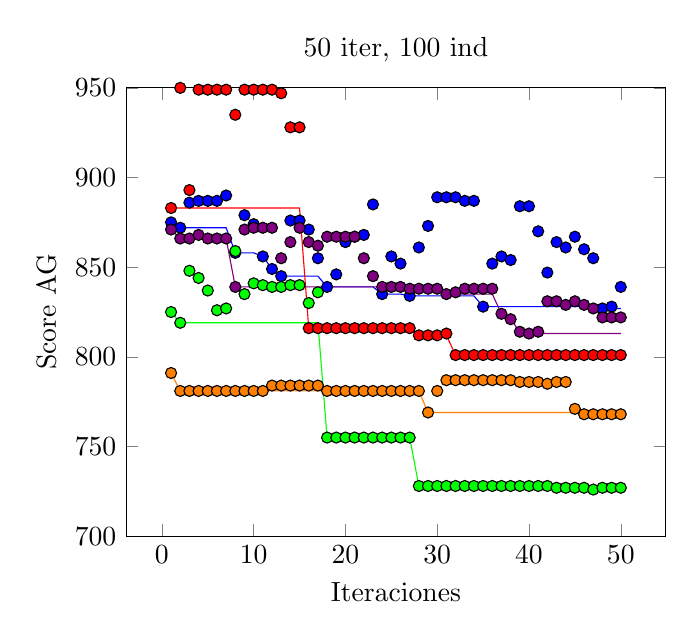
\begin{tikzpicture}
      \begin{axis}[
      title={50 iter, 100 ind},
      xlabel={Iteraciones},
      ylabel={Score AG},
      ymin=700,ymax=950]
      
      \addplot[color=blue] coordinates {(1,875)(2,872)(7,872)(8,858)(10,858)(11,856)(12,849)(13,845)(17,845)(18,839)(23,839)(24,835)(26,835)(27,834)(34,834)(35,828)(47,828)(48,827)(50,827)};
      \addplot[only marks, mark options={fill=blue}] coordinates {(1,875)(2,872)(3,886)(4,887)(5,887)(6,887)(7,890)(8,858)(9,879)(10,874)(11,856)(12,849)(13,845)(14,876)(15,876)(16,871)(17,855)(18,839)(19,846)(20,864)(21,867)(22,868)(23,885)(24,835)(25,856)(26,852)(27,834)(28,861)(29,873)(30,889)(31,889)(32,889)(33,887)(34,887)(35,828)(36,852)(37,856)(38,854)(39,884)(40,884)(41,870)(42,847)(43,864)(44,861)(45,867)(46,860)(47,855)(48,827)(49,828)(50,839)};
      
      \addplot[color=red] coordinates {(1,883)(15,883)(16,816)(27,816)(28,812)(31,812)(32,801)(50,801)};
      \addplot[only marks, mark options={fill=red}] coordinates {(1,883)(2,950)(3,893)(4,949)(5,949)(6,949)(7,949)(8,935)(9,949)(10,949)(11,949)(12,949)(13,947)(14,928)(15,928)(16,816)(17,816)(18,816)(19,816)(20,816)(21,816)(22,816)(23,816)(24,816)(25,816)(26,816)(27,816)(28,812)(29,812)(30,812)(31,813)(32,801)(33,801)(34,801)(35,801)(36,801)(37,801)(38,801)(39,801)(40,801)(41,801)(42,801)(43,801)(44,801)(45,801)(46,801)(47,801)(48,801)(49,801)(50,801)};
      
      \addplot[color=green] coordinates {(1,825)(2,819)(17,819)(18,755)(27,755)(28,728)(42,728)(43,727)(46,727)(47,726)(50,726)};
      \addplot[only marks, mark options={fill=green}] coordinates {(1,825)(2,819)(3,848)(4,844)(5,837)(6,826)(7,827)(8,859)(9,835)(10,841)(11,840)(12,839)(13,839)(14,840)(15,840)(16,830)(17,836)(18,755)(19,755)(20,755)(21,755)(22,755)(23,755)(24,755)(25,755)(26,755)(27,755)(28,728)(29,728)(30,728)(31,728)(32,728)(33,728)(34,728)(35,728)(36,728)(37,728)(38,728)(39,728)(40,728)(41,728)(42,728)(43,727)(44,727)(45,727)(46,727)(47,726)(48,727)(49,727)(50,727)};
      
      \addplot[color=orange] coordinates{(1,791)(2,781)(28,781)(29,769)(45,769)(46,768)(50,768)};
      \addplot[only marks, mark options={fill=orange}] coordinates {(1,791)(2,781)(3,781)(4,781)(5,781)(6,781)(7,781)(8,781)(9,781)(10,781)(11,781)(12,784)(13,784)(14,784)(15,784)(16,784)(17,784)(18,781)(19,781)(20,781)(21,781)(22,781)(23,781)(24,781)(25,781)(26,781)(27,781)(28,781)(29,769)(30,781)(31,787)(32,787)(33,787)(34,787)(35,787)(36,787)(37,787)(38,787)(39,786)(40,786)(41,786)(42,785)(43,786)(44,786)(45,771)(46,768)(47,768)(48,768)(49,768)(50,768)};
      
      \addplot[color=violet] coordinates {(1,871)(2,866)(7,866)(8,839)(26,839)(27,838)(30,838)(31,835)(36,835)(37,824)(38,821)(39,814)(40,813)(50,813)};
      \addplot[only marks, mark options={fill=violet}] coordinates {(1,871)(2,866)(3,866)(4,868)(5,866)(6,866)(7,866)(8,839)(9,871)(10,872)(11,872)(12,872)(13,855)(14,864)(15,872)(16,864)(17,862)(18,867)(19,867)(20,867)(21,867)(22,855)(23,845)(24,839)(25,839)(26,839)(27,838)(28,838)(29,838)(30,838)(31,835)(32,836)(33,838)(34,838)(35,838)(36,838)(37,824)(38,821)(39,814)(40,813)(41,814)(42,831)(43,831)(44,829)(45,831)(46,829)(47,827)(48,822)(49,822)(50,822)};
      
      \end{axis}
\end{tikzpicture}}
\end{subfigure}
% FIGURE 27
\begin{subfigure}[b]{0.43\textwidth}
\resizebox{\linewidth}{!}{
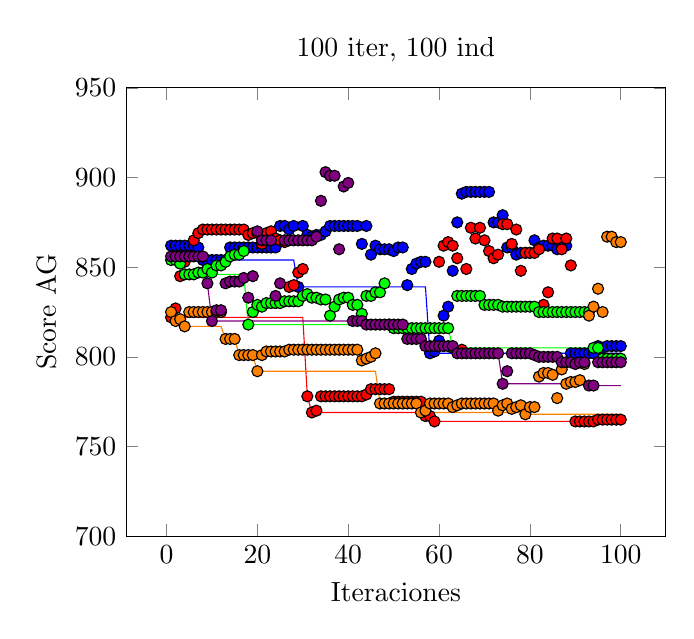
\begin{tikzpicture}
      \begin{axis}[
      title={100 iter, 100 ind},
      xlabel={Iteraciones},
      ylabel={Score AG},
      ymin=700,ymax=950]
      
      \addplot[color=blue] coordinates {(1,861)(7,861)(8,854)(28,854)(29,839)(57,839)(58,802)(100,802)};
      \addplot[only marks, mark options={fill=blue}] coordinates {(1,862)(2,862)(3,862)(4,862)(5,862)(6,862)(7,861)(8,854)(9,854)(10,854)(11,854)(12,854)(13,854)(14,861)(15,861)(16,861)(17,861)(18,861)(19,861)(20,861)(21,861)(22,861)(23,861)(24,861)(25,873)(26,873)(27,871)(28,873)(29,839)(30,873)(31,868)(32,867)(33,868)(34,868)(35,870)(36,873)(37,873)(38,873)(39,873)(40,873)(41,873)(42,873)(43,863)(44,873)(45,857)(46,862)(47,860)(48,860)(49,860)(50,859)(51,861)(52,861)(53,840)(54,849)(55,852)(56,853)(57,853)(58,802)(59,803)(60,809)(61,823)(62,828)(63,848)(64,875)(65,891)(66,892)(67,892)(68,892)(69,892)(70,892)(71,892)(72,875)(73,875)(74,879)(75,861)(76,861)(77,857)(78,858)(79,858)(80,858)(81,865)(82,861)(83,862)(84,862)(85,862)(86,860)(87,861)(88,862)(89,802)(90,802)(91,802)(92,802)(93,802)(94,802)(95,806)(96,805)(97,806)(98,806)(99,806)(100,806)};
      
      \addplot[color=red] coordinates {(1,822)(30,822)(31,778)(32,769)(56,769)(57,767)(58,767)(59,764)(100,764)};
      \addplot[only marks, mark options={fill=red}] coordinates {(1,822)(2,827)(3,845)(4,853)(5,856)(6,865)(7,869)(8,871)(9,871)(10,871)(11,871)(12,871)(13,871)(14,871)(15,871)(16,871)(17,871)(18,868)(19,869)(20,869)(21,863)(22,869)(23,870)(24,866)(25,865)(26,864)(27,839)(28,840)(29,847)(30,849)(31,778)(32,769)(33,770)(34,778)(35,778)(36,778)(37,778)(38,778)(39,778)(40,778)(41,778)(42,778)(43,778)(44,779)(45,782)(46,782)(47,782)(48,782)(49,782)(50,775)(51,775)(52,775)(53,775)(54,775)(55,775)(56,775)(57,767)(58,767)(59,764)(60,853)(61,862)(62,864)(63,862)(64,855)(65,804)(66,849)(67,872)(68,866)(69,872)(70,865)(71,859)(72,855)(73,857)(74,874)(75,874)(76,863)(77,871)(78,848)(79,858)(80,858)(81,858)(82,860)(83,829)(84,836)(85,866)(86,866)(87,860)(88,866)(89,851)(90,764)(91,764)(92,764)(93,764)(94,764)(95,765)(96,765)(97,765)(98,765)(99,765)(100,765)};
      
      \addplot[color=green] coordinates {(1,854)(2,854)(3,852)(4,846)(17,846)(18,818)(49,818)(50,816)(62,816)(63,805)(95,805)(96,799)(100,799)};
      \addplot[only marks, mark options={fill=green}] coordinates {(1,854)(2,854)(3,852)(4,846)(5,846)(6,846)(7,847)(8,847)(9,849)(10,847)(11,851)(12,851)(13,853)(14,856)(15,857)(16,857)(17,859)(18,818)(19,825)(20,829)(21,828)(22,830)(23,830)(24,830)(25,830)(26,831)(27,831)(28,831)(29,831)(30,834)(31,835)(32,833)(33,833)(34,832)(35,832)(36,823)(37,828)(38,832)(39,833)(40,833)(41,829)(42,829)(43,824)(44,834)(45,834)(46,836)(47,836)(48,841)(49,818)(50,816)(51,816)(52,816)(53,816)(54,816)(55,816)(56,816)(57,816)(58,816)(59,816)(60,816)(61,816)(62,816)(63,805)(64,834)(65,834)(66,834)(67,834)(68,834)(69,834)(70,829)(71,829)(72,829)(73,829)(74,828)(75,828)(76,828)(77,828)(78,828)(79,828)(80,828)(81,828)(82,825)(83,825)(84,825)(85,825)(86,825)(87,825)(88,825)(89,825)(90,825)(91,825)(92,825)(93,825)(94,805)(95,805)(96,799)(97,799)(98,799)(99,799)(100,799)};
      
      \addplot[color=orange] coordinates{(1,825)(2,820)(3,820)(4,817)(12,817)(13,810)(15,810)(16,801)(19,801)(20,792)(46,792)(47,774)(55,774)(56,769)(78,769)(79,768)(100,768)};
      \addplot[only marks, mark options={fill=orange}] coordinates {(1,825)(2,820)(3,821)(4,817)(5,825)(6,825)(7,825)(8,825)(9,825)(10,825)(11,825)(12,825)(13,810)(14,810)(15,810)(16,801)(17,801)(18,801)(19,801)(20,792)(21,801)(22,803)(23,803)(24,803)(25,803)(26,803)(27,804)(28,804)(29,804)(30,804)(31,804)(32,804)(33,804)(34,804)(35,804)(36,804)(37,804)(38,804)(39,804)(40,804)(41,804)(42,804)(43,798)(44,799)(45,800)(46,802)(47,774)(48,774)(49,774)(50,774)(51,774)(52,774)(53,774)(54,774)(55,774)(56,769)(57,770)(58,774)(59,774)(60,774)(61,774)(62,774)(63,772)(64,773)(65,774)(66,774)(67,774)(68,774)(69,774)(70,774)(71,774)(72,774)(73,770)(74,773)(75,774)(76,771)(77,772)(78,773)(79,768)(80,772)(81,772)(82,789)(83,791)(84,791)(85,790)(86,777)(87,793)(88,785)(89,786)(90,786)(91,787)(92,796)(93,823)(94,828)(95,838)(96,825)(97,867)(98,867)(99,864)(100,864)};
      
      \addplot[color=violet] coordinates {(1,856)(8,856)(9,841)(10,820)(43,820)(44,818)(52,818)(53,810)(56,810)(57,806)(63,806)(64,802)(73,802)(74,785)(92,785)(93,784)(100,784)};
      \addplot[only marks, mark options={fill=violet}] coordinates {(1,856)(2,856)(3,856)(4,856)(5,856)(6,856)(7,856)(8,856)(9,841)(10,820)(11,826)(12,826)(13,841)(14,842)(15,842)(16,842)(17,844)(18,833)(19,845)(20,870)(21,865)(22,865)(23,865)(24,834)(25,841)(26,865)(27,865)(28,865)(29,865)(30,865)(31,865)(32,865)(33,867)(34,887)(35,903)(36,901)(37,901)(38,860)(39,895)(40,897)(41,820)(42,820)(43,820)(44,818)(45,818)(46,818)(47,818)(48,818)(49,818)(50,818)(51,818)(52,818)(53,810)(54,810)(55,810)(56,810)(57,806)(58,806)(59,806)(60,806)(61,806)(62,806)(63,806)(64,802)(65,802)(66,802)(67,802)(68,802)(69,802)(70,802)(71,802)(72,802)(73,802)(74,785)(75,792)(76,802)(77,802)(78,802)(79,802)(80,802)(81,801)(82,800)(83,800)(84,800)(85,800)(86,800)(87,797)(88,797)(89,797)(90,796)(91,797)(92,797)(93,784)(94,784)(95,797)(96,797)(97,797)(98,797)(99,797)(100,797)};
      
      \end{axis}
\end{tikzpicture}}
\end{subfigure}
\newline
\centering
% FIGURE 28
\begin{subfigure}[b]{0.43\textwidth}
\resizebox{\linewidth}{!}{
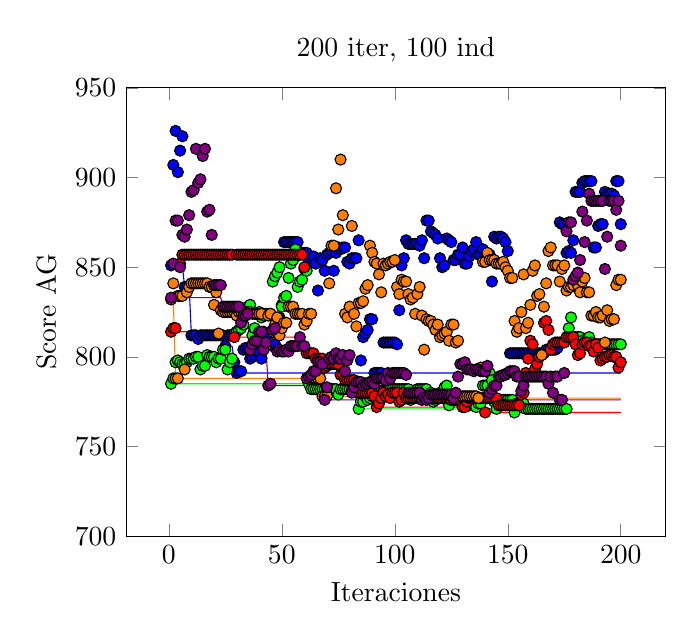
\begin{tikzpicture}
      \begin{axis}[
      title={200 iter, 100 ind},
      xlabel={Iteraciones},
      ylabel={Score AG},
      ymin=700,ymax=950]
      
      \addplot[color=blue] coordinates {(1,851)(6,851)(7,839)(9,839)(10,812)(12,812)(13,810)(24,810)(25,806)(28,806)(29,797)(30,791)(200,791)};
      \addplot[only marks, mark options={fill=blue}] coordinates {(1,851)(2,907)(3,926)(4,903)(5,915)(6,923)(7,839)(8,839)(9,839)(10,812)(11,812)(12,812)(13,810)(14,812)(15,812)(16,812)(17,812)(18,812)(19,812)(20,812)(21,812)(22,812)(23,812)(24,812)(25,806)(26,812)(27,812)(28,812)(29,797)(30,791)(31,792)(32,792)(33,804)(34,805)(35,805)(36,799)(37,800)(38,801)(39,803)(40,803)(41,799)(42,814)(43,813)(44,813)(45,813)(46,806)(47,807)(48,814)(49,822)(50,829)(51,864)(52,864)(53,864)(54,864)(55,864)(56,864)(57,864)(58,857)(59,858)(60,858)(61,858)(62,853)(63,855)(64,856)(65,852)(66,837)(67,855)(68,854)(69,848)(70,857)(71,858)(72,859)(73,848)(74,858)(75,861)(76,860)(77,861)(78,861)(79,853)(80,852)(81,855)(82,855)(83,855)(84,865)(85,798)(86,811)(87,813)(88,815)(89,821)(90,821)(91,791)(92,791)(93,791)(94,791)(95,808)(96,808)(97,808)(98,808)(99,808)(100,808)(101,807)(102,826)(103,851)(104,855)(105,865)(106,863)(107,863)(108,863)(109,863)(110,863)(111,862)(112,865)(113,855)(114,876)(115,876)(116,870)(117,869)(118,868)(119,866)(120,855)(121,850)(122,851)(123,866)(124,865)(125,864)(126,854)(127,854)(128,857)(129,857)(130,861)(131,852)(132,852)(133,856)(134,859)(135,860)(136,864)(137,857)(138,857)(139,860)(140,856)(141,856)(142,857)(143,842)(144,867)(145,866)(146,867)(147,867)(148,866)(149,864)(150,859)(151,802)(152,802)(153,802)(154,802)(155,802)(156,802)(157,802)(158,802)(159,802)(160,802)(161,802)(162,802)(163,802)(164,802)(165,802)(166,802)(167,804)(168,804)(169,804)(170,804)(171,804)(172,805)(173,875)(174,874)(175,874)(176,858)(177,859)(178,858)(179,865)(180,892)(181,892)(182,892)(183,897)(184,898)(185,898)(186,898)(187,898)(188,861)(189,861)(190,873)(191,874)(192,874)(193,892)(194,891)(195,891)(196,891)(197,890)(198,898)(199,898)(200,874)};
      
      \addplot[color=green] coordinates {(1,785)(62,785)(63,782)(74,782)(75,779)(83,779)(84,771)(152,771)(153,769)(200,769)};
      \addplot[only marks, mark options={fill=green}] coordinates {(1,785)(2,788)(3,797)(4,798)(5,797)(6,796)(7,796)(8,797)(9,799)(10,799)(11,799)(12,800)(13,800)(14,793)(15,795)(16,795)(17,801)(18,800)(19,800)(20,800)(21,797)(22,799)(23,799)(24,804)(25,804)(26,793)(27,797)(28,799)(29,813)(30,814)(31,815)(32,816)(33,818)(34,826)(35,828)(36,829)(37,812)(38,816)(39,824)(40,825)(41,822)(42,823)(43,824)(44,824)(45,824)(46,842)(47,845)(48,847)(49,850)(50,828)(51,833)(52,834)(53,844)(54,852)(55,854)(56,860)(57,839)(58,842)(59,843)(60,849)(61,848)(62,785)(63,782)(64,782)(65,782)(66,782)(67,782)(68,782)(69,782)(70,782)(71,782)(72,782)(73,782)(74,782)(75,779)(76,782)(77,782)(78,782)(79,782)(80,782)(81,782)(82,782)(83,782)(84,771)(85,775)(86,775)(87,778)(88,776)(89,777)(90,778)(91,779)(92,780)(93,781)(94,781)(95,781)(96,781)(97,781)(98,782)(99,782)(100,782)(101,782)(102,782)(103,782)(104,782)(105,782)(106,782)(107,776)(108,779)(109,780)(110,782)(111,782)(112,782)(113,782)(114,782)(115,779)(116,780)(117,775)(118,776)(119,777)(120,780)(121,777)(122,783)(123,784)(124,773)(125,776)(126,778)(127,778)(128,778)(129,775)(130,777)(131,774)(132,776)(133,773)(134,774)(135,774)(136,772)(137,774)(138,774)(139,784)(140,784)(141,784)(142,791)(143,787)(144,775)(145,771)(146,776)(147,776)(148,776)(149,776)(150,776)(151,776)(152,776)(153,769)(154,774)(155,774)(156,774)(157,774)(158,771)(159,771)(160,771)(161,771)(162,771)(163,771)(164,771)(165,771)(166,771)(167,771)(168,771)(169,771)(170,771)(171,771)(172,771)(173,771)(174,771)(175,771)(176,771)(177,816)(178,822)(179,811)(180,811)(181,811)(182,811)(183,809)(184,807)(185,810)(186,811)(187,808)(188,807)(189,807)(190,807)(191,807)(192,807)(193,807)(194,807)(195,807)(196,807)(197,807)(198,807)(199,807)(200,807)};
      
      \addplot[color=red] coordinates {(1,814)(28,814)(29,811)(60,811)(61,802)(64,802)(65,799)(68,799)(69,794)(75,794)(76,790)(77,790)(78,787)(82,787)(83,780)(90,780)(91,778)(92,772)(139,772)(140,769)(200,769)};
      \addplot[only marks, mark options={fill=red}] coordinates {(1,814)(2,816)(3,816)(4,834)(5,852)(6,857)(7,857)(8,857)(9,857)(10,857)(11,857)(12,857)(13,857)(14,857)(15,857)(16,857)(17,857)(18,857)(19,857)(20,857)(21,857)(22,857)(23,857)(24,857)(25,857)(26,857)(27,857)(28,857)(29,811)(30,857)(31,857)(32,857)(33,857)(34,857)(35,857)(36,857)(37,857)(38,857)(39,857)(40,857)(41,857)(42,857)(43,857)(44,857)(45,857)(46,857)(47,857)(48,857)(49,857)(50,857)(51,857)(52,857)(53,857)(54,857)(55,857)(56,857)(57,857)(58,857)(59,857)(60,850)(61,802)(62,802)(63,802)(64,802)(65,799)(66,799)(67,799)(68,799)(69,794)(70,795)(71,796)(72,796)(73,796)(74,796)(75,796)(76,790)(77,790)(78,787)(79,787)(80,787)(81,787)(82,787)(83,780)(84,780)(85,780)(86,780)(87,780)(88,780)(89,780)(90,780)(91,778)(92,772)(93,774)(94,777)(95,780)(96,778)(97,779)(98,777)(99,780)(100,780)(101,780)(102,775)(103,776)(104,780)(105,777)(106,777)(107,777)(108,777)(109,777)(110,777)(111,777)(112,777)(113,777)(114,777)(115,777)(116,777)(117,777)(118,777)(119,777)(120,777)(121,777)(122,777)(123,777)(124,777)(125,776)(126,776)(127,776)(128,776)(129,776)(130,772)(131,772)(132,775)(133,777)(134,777)(135,777)(136,777)(137,777)(138,777)(139,777)(140,769)(141,777)(142,777)(143,777)(144,777)(145,777)(146,773)(147,773)(148,773)(149,773)(150,773)(151,773)(152,773)(153,773)(154,773)(155,773)(156,779)(157,780)(158,791)(159,799)(160,809)(161,807)(162,793)(163,796)(164,800)(165,801)(166,819)(167,820)(168,815)(169,804)(170,807)(171,808)(172,808)(173,808)(174,808)(175,808)(176,811)(177,811)(178,811)(179,811)(180,807)(181,801)(182,802)(183,807)(184,808)(185,808)(186,806)(187,806)(188,803)(189,807)(190,805)(191,798)(192,799)(193,800)(194,800)(195,801)(196,801)(197,800)(198,800)(199,794)(200,797)};
      
      \addplot[color=orange] coordinates {(1,832)(2,832)(3,788)(67,788)(68,778)(136,778)(137,777)(200,777)};
      \addplot[only marks, mark options={fill=orange}] coordinates {(1,832)(2,841)(3,788)(4,788)(5,834)(6,834)(7,793)(8,836)(9,839)(10,841)(11,841)(12,841)(13,841)(14,841)(15,841)(16,841)(17,841)(18,839)(19,839)(20,829)(21,836)(22,813)(23,826)(24,825)(25,825)(26,825)(27,825)(28,825)(29,825)(30,823)(31,825)(32,825)(33,825)(34,825)(35,825)(36,825)(37,824)(38,824)(39,824)(40,824)(41,824)(42,807)(43,806)(44,823)(45,824)(46,814)(47,818)(48,822)(49,812)(50,816)(51,819)(52,819)(53,828)(54,828)(55,828)(56,824)(57,824)(58,824)(59,824)(60,818)(61,820)(62,824)(63,824)(64,788)(65,788)(66,788)(67,788)(68,778)(69,778)(70,778)(71,841)(72,862)(73,862)(74,894)(75,871)(76,910)(77,879)(78,824)(79,822)(80,828)(81,873)(82,824)(83,817)(84,830)(85,830)(86,831)(87,838)(88,840)(89,862)(90,858)(91,853)(92,852)(93,846)(94,836)(95,852)(96,851)(97,852)(98,853)(99,853)(100,854)(101,839)(102,835)(103,843)(104,842)(105,842)(106,835)(107,832)(108,833)(109,824)(110,835)(111,839)(112,823)(113,804)(114,821)(115,820)(116,820)(117,818)(118,815)(119,818)(120,811)(121,812)(122,813)(123,814)(124,809)(125,818)(126,818)(127,808)(128,809)(129,778)(130,778)(131,778)(132,778)(133,778)(134,778)(135,778)(136,778)(137,777)(138,794)(139,853)(140,853)(141,858)(142,854)(143,854)(144,854)(145,852)(146,852)(147,852)(148,853)(149,850)(150,848)(151,844)(152,844)(153,820)(154,814)(155,816)(156,825)(157,846)(158,816)(159,819)(160,829)(161,848)(162,851)(163,834)(164,835)(165,801)(166,828)(167,841)(168,859)(169,861)(170,851)(171,851)(172,851)(173,842)(174,849)(175,851)(176,837)(177,839)(178,839)(179,840)(180,843)(181,840)(182,836)(183,842)(184,844)(185,836)(186,836)(187,823)(188,823)(189,825)(190,822)(191,822)(192,823)(193,808)(194,826)(195,820)(196,821)(197,821)(198,840)(199,843)(200,843)};
      
      \addplot[color=violet] coordinates {(1,833)(23,833)(24,828)(31,828)(32,819)(35,819)(36,804)(43,804)(44,784)(68,784)(69,776)(200,776)};
      \addplot[only marks, mark options={fill=violet}] coordinates {(1,833)(2,852)(3,876)(4,876)(5,850)(6,868)(7,867)(8,871)(9,879)(10,892)(11,893)(12,916)(13,897)(14,899)(15,912)(16,916)(17,881)(18,882)(19,868)(20,840)(21,840)(22,840)(23,840)(24,828)(25,828)(26,828)(27,828)(28,828)(29,828)(30,828)(31,828)(32,819)(33,823)(34,823)(35,824)(36,804)(37,807)(38,809)(39,809)(40,814)(41,814)(42,804)(43,808)(44,784)(45,785)(46,815)(47,816)(48,803)(49,804)(50,803)(51,803)(52,804)(53,803)(54,806)(55,806)(56,806)(57,806)(58,811)(59,806)(60,806)(61,788)(62,789)(63,790)(64,792)(65,792)(66,797)(67,797)(68,796)(69,776)(70,783)(71,799)(72,800)(73,799)(74,802)(75,799)(76,799)(77,801)(78,792)(79,798)(80,801)(81,780)(82,783)(83,786)(84,786)(85,786)(86,784)(87,785)(88,785)(89,786)(90,786)(91,785)(92,788)(93,788)(94,788)(95,788)(96,787)(97,791)(98,788)(99,791)(100,791)(101,791)(102,791)(103,791)(104,791)(105,790)(106,780)(107,780)(108,780)(109,780)(110,780)(111,780)(112,776)(113,777)(114,776)(115,777)(116,779)(117,779)(118,779)(119,779)(120,779)(121,779)(122,779)(123,779)(124,779)(125,779)(126,777)(127,780)(128,789)(129,796)(130,796)(131,797)(132,793)(133,793)(134,793)(135,792)(136,793)(137,793)(138,792)(139,792)(140,792)(141,795)(142,780)(143,782)(144,784)(145,784)(146,789)(147,789)(148,790)(149,790)(150,791)(151,792)(152,792)(153,792)(154,789)(155,789)(156,781)(157,784)(158,789)(159,789)(160,789)(161,789)(162,789)(163,789)(164,789)(165,789)(166,789)(167,789)(168,785)(169,789)(170,780)(171,789)(172,789)(173,776)(174,776)(175,791)(176,870)(177,875)(178,875)(179,843)(180,845)(181,847)(182,854)(183,881)(184,864)(185,876)(186,891)(187,887)(188,887)(189,887)(190,887)(191,887)(192,887)(193,849)(194,867)(195,887)(196,887)(197,887)(198,882)(199,887)(200,862)};
      
      \end{axis}
\end{tikzpicture}}
\end{subfigure}
\caption{Ejecuciones del modelo avanzado con métrica basada en tiempo (100 ind.)}
\label{fig:adv_simulation_time_res_100}
\end{figure}

Como se puede ver en la figura \ref{fig:adv_simulation_time_res_100}, por lo general, los resultados obtenidos son bastante diferentes de los obtenidos en las pruebas anteriores basadas en las métricas centradas en el consumo eléctrico. En estos resultados, se puede ver como el aprendizaje del sistema es bastante menor al observado originalmente, apareciendo de nuevo los casos en el que los mejores valores de una iteración empeoran conforme avanzan las iteraciones, aunque, en todo caso, en una medida mucho menor de lo observado en el modelo básico.

Esta diferencia respecto al modelo básico se puede ver reflejada claramente en la tabla \ref{tab:adv_simulation_time}, donde el coeficiente de variación es prácticamente similar al obtenido en las primeras pruebas del modelo avanzado, de las tablas \ref{tab:adv_simulation_cv_30} y \ref{tab:adv_simulation_cv_100}. De esta misma tabla es posible extraer el hecho que, al igual que ocurre con las métricas centradas en el consumo eléctrico, el dedicarle una cantidad mayor de iteraciones (200 en comparación a 100), no implica una mejora sustancial de los resultados, más allá de posibles resultados individuales dentro de alguna de las repeticiones realizadas que destaquen, tanto para bien como para mal en los resultados obtenidos.

\begin{table}[!htb]
    \centering
    \begin{tabular}{m{0.15\textwidth}*3c}
    \toprule
    \multirow{3}*{\textbf{Medida}} & \multicolumn{3}{c}{\textbf{Modelo avanzado}} \\
     & \textbf{50 it.} & \textbf{100 it.} & \textbf{200 it.} \\
    \midrule
    \textbf{Desviación típica} & 22,999 & 25,397 & 28,637 \\
    \textbf{Media} & 820 & 826 & 816 \\
    \textbf{Coeficiente de variación} & 2,80\% & 3,08\% & 3,51\% \\
    \bottomrule
    \end{tabular}
    \caption{Valores de dispersión basados en tiempo (100 ind.)}
    \label{tab:adv_simulation_time}
\end{table}

Otra de las pruebas realizadas, siguiendo la misma estela de las métricas basadas en la mejora de los consumos se trata de poder observar si un margen diferente entre los puntos implica un cambio sustancial en los resultados. Los resultados de estas ejecuciones se pueden observar en la figura \ref{fig:adv_multi_margin_time}. En este caso, al igual que en las pruebas anteriores, cada serie de la figura representa, en cada iteración, la media de las puntuaciones del mejor individuo obtenido hasta dicho momento entre las 5 ejecuciones realizadas por cada valor de margen a probar.

% FIGURE 29
\begin{figure}[!htb]
    \centering
    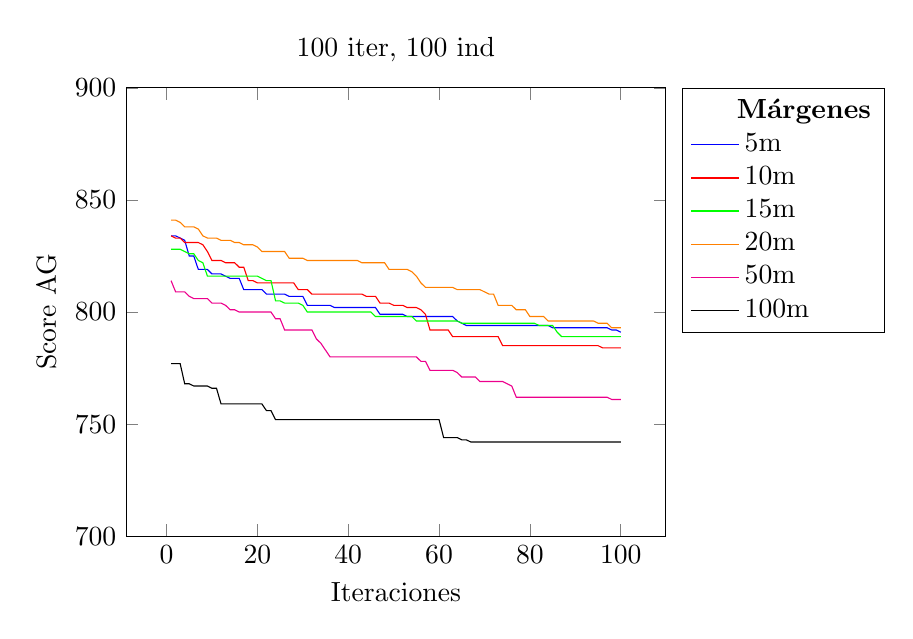
\begin{tikzpicture}
      \begin{axis}[
      title={100 iter, 100 ind},
      xlabel={Iteraciones},
      ylabel={Score AG},
      ymin=700,ymax=900,
      legend cell align={left},
      legend pos=outer north east]
      
      \addlegendimage{empty legend}
      
      %\addplot[color=blue] coordinates {(1,842)(2,842)(3,842)(4,841)(5,834)(6,836)(7,830)(8,838)(9,837)(10,831)(11,833)(12,836)(13,832)(14,832)(15,833)(16,836)(17,832)(18,835)(19,835)(20,835)(21,838)(22,829)(23,839)(24,836)(25,836)(26,842)(27,835)(28,840)(29,832)(30,831)(31,816)(32,817)(33,818)(34,821)(35,822)(36,819)(37,817)(38,814)(39,814)(40,820)(41,822)(42,830)(43,829)(44,828)(45,819)(46,820)(47,818)(48,814)(49,809)(50,815)(51,815)(52,816)(53,816)(54,815)(55,815)(56,813)(57,813)(58,807)(59,809)(60,813)(61,816)(62,816)(63,811)(64,810)(65,813)(66,809)(67,807)(68,807)(69,807)(70,808)(71,812)(72,818)(73,817)(74,820)(75,820)(76,820)(77,817)(78,816)(79,818)(80,819)(81,819)(82,813)(83,814)(84,812)(85,805)(86,809)(87,820)(88,815)(89,814)(90,815)(91,823)(92,823)(93,823)(94,822)(95,825)(96,827)(97,807)(98,807)(99,808)(100,801)};
      
      %\addplot[color=red] coordinates {(1,844)(2,844)(3,847)(4,847)(5,849)(6,851)(7,852)(8,851)(9,848)(10,844)(11,845)(12,846)(13,846)(14,848)(15,848)(16,846)(17,847)(18,836)(19,840)(20,844)(21,844)(22,846)(23,846)(24,839)(25,843)(26,847)(27,842)(28,843)(29,837)(30,845)(31,830)(32,827)(33,828)(34,833)(35,837)(36,835)(37,836)(38,829)(39,836)(40,836)(41,821)(42,821)(43,817)(44,821)(45,818)(46,820)(47,814)(48,815)(49,810)(50,808)(51,809)(52,809)(53,803)(54,805)(55,805)(56,804)(57,802)(58,793)(59,793)(60,812)(61,816)(62,817)(63,818)(64,828)(65,821)(66,830)(67,834)(68,833)(69,834)(70,832)(71,831)(72,827)(73,826)(74,827)(75,825)(76,825)(77,826)(78,822)(79,823)(80,823)(81,825)(82,827)(83,821)(84,823)(85,828)(86,825)(87,827)(88,827)(89,812)(90,795)(91,795)(92,797)(93,800)(94,797)(95,802)(96,798)(97,807)(98,807)(99,806)(100,806)};
      
      %\addplot[color=green] coordinates {(1,828)(2,845)(3,851)(4,855)(5,845)(6,847)(7,830)(8,839)(9,831)(10,837)(11,833)(12,839)(13,839)(14,846)(15,845)(16,851)(17,843)(18,848)(19,839)(20,838)(21,830)(22,826)(23,836)(24,826)(25,828)(26,826)(27,821)(28,830)(29,829)(30,829)(31,816)(32,821)(33,819)(34,816)(35,813)(36,813)(37,813)(38,812)(39,816)(40,816)(41,819)(42,820)(43,818)(44,816)(45,816)(46,813)(47,814)(48,814)(49,815)(50,815)(51,813)(52,802)(53,802)(54,805)(55,803)(56,804)(57,810)(58,807)(59,807)(60,807)(61,804)(62,805)(63,801)(64,802)(65,803)(66,805)(67,807)(68,813)(69,813)(70,808)(71,819)(72,815)(73,814)(74,810)(75,806)(76,808)(77,810)(78,815)(79,815)(80,811)(81,807)(82,804)(83,803)(84,802)(85,803)(86,803)(87,801)(88,804)(89,803)(90,803)(91,802)(92,802)(93,803)(94,803)(95,803)(96,803)(97,803)(98,803)(99,803)(100,803)};
      
      %\addplot[color=orange] coordinates {(1,847)(2,848)(3,846)(4,841)(5,841)(6,842)(7,840)(8,836)(9,839)(10,841)(11,842)(12,839)(13,835)(14,836)(15,836)(16,835)(17,832)(18,836)(19,835)(20,833)(21,827)(22,829)(23,833)(24,831)(25,839)(26,841)(27,841)(28,836)(29,836)(30,840)(31,843)(32,855)(33,849)(34,871)(35,870)(36,874)(37,869)(38,884)(39,887)(40,874)(41,867)(42,868)(43,861)(44,865)(45,853)(46,850)(47,849)(48,851)(49,840)(50,846)(51,841)(52,840)(53,839)(54,834)(55,836)(56,836)(57,832)(58,830)(59,823)(60,833)(61,832)(62,837)(63,832)(64,829)(65,832)(66,832)(67,832)(68,833)(69,833)(70,829)(71,826)(72,829)(73,823)(74,825)(75,826)(76,826)(77,821)(78,826)(79,828)(80,819)(81,817)(82,816)(83,821)(84,825)(85,832)(86,828)(87,822)(88,821)(89,821)(90,821)(91,822)(92,824)(93,820)(94,818)(95,820)(96,822)(97,823)(98,828)(99,833)(100,832)};
      
      %\addplot[color=magenta] coordinates {(1,814)(2,816)(3,823)(4,822)(5,825)(6,824)(7,827)(8,828)(9,829)(10,831)(11,843)(12,842)(13,841)(14,824)(15,825)(16,827)(17,839)(18,843)(19,843)(20,837)(21,836)(22,839)(23,839)(24,832)(25,838)(26,840)(27,845)(28,852)(29,845)(30,846)(31,844)(32,845)(33,830)(34,828)(35,821)(36,824)(37,825)(38,825)(39,824)(40,847)(41,844)(42,841)(43,838)(44,832)(45,830)(46,830)(47,821)(48,828)(49,825)(50,826)(51,825)(52,826)(53,830)(54,834)(55,814)(56,820)(57,795)(58,790)(59,791)(60,797)(61,797)(62,795)(63,801)(64,800)(65,792)(66,792)(67,789)(68,784)(69,784)(70,785)(71,784)(72,789)(73,788)(74,787)(75,780)(76,778)(77,771)(78,775)(79,776)(80,782)(81,782)(82,781)(83,782)(84,782)(85,782)(86,779)(87,774)(88,774)(89,776)(90,776)(91,776)(92,772)(93,771)(94,771)(95,771)(96,773)(97,773)(98,768)(99,773)(100,775)};
      
      %\addplot[color=black] coordinates {(1,781)(2,789)(3,796)(4,792)(5,783)(6,782)(7,797)(8,797)(9,797)(10,796)(11,796)(12,790)(13,790)(14,790)(15,790)(16,790)(17,790)(18,790)(19,790)(20,790)(21,790)(22,787)(23,795)(24,791)(25,788)(26,787)(27,787)(28,789)(29,791)(30,789)(31,771)(32,772)(33,780)(34,780)(35,782)(36,782)(37,782)(38,784)(39,797)(40,809)(41,814)(42,810)(43,800)(44,801)(45,798)(46,798)(47,811)(48,811)(49,810)(50,816)(51,814)(52,814)(53,801)(54,801)(55,791)(56,791)(57,802)(58,808)(59,818)(60,819)(61,791)(62,793)(63,791)(64,796)(65,800)(66,807)(67,818)(68,820)(69,820)(70,821)(71,821)(72,816)(73,820)(74,812)(75,812)(76,812)(77,811)(78,826)(79,822)(80,822)(81,820)(82,816)(83,823)(84,812)(85,824)(86,825)(87,815)(88,819)(89,839)(90,854)(91,860)(92,860)(93,837)(94,840)(95,840)(96,811)(97,804)(98,788)(99,792)(100,792)};
      
        
        
      \addplot[color=blue] coordinates {(1,834)(2,834)(3,833)(4,832)(5,825)(6,825)(7,819)(8,819)(9,819)(10,817)(11,817)(12,817)(13,816)(14,815)(15,815)(16,815)(17,810)(18,810)(19,810)(20,810)(21,810)(22,808)(23,808)(24,808)(25,808)(26,808)(27,807)(28,807)(29,807)(30,807)(31,803)(32,803)(33,803)(34,803)(35,803)(36,803)(37,802)(38,802)(39,802)(40,802)(41,802)(42,802)(43,802)(44,802)(45,802)(46,802)(47,799)(48,799)(49,799)(50,799)(51,799)(52,799)(53,798)(54,798)(55,798)(56,798)(57,798)(58,798)(59,798)(60,798)(61,798)(62,798)(63,798)(64,796)(65,795)(66,794)(67,794)(68,794)(69,794)(70,794)(71,794)(72,794)(73,794)(74,794)(75,794)(76,794)(77,794)(78,794)(79,794)(80,794)(81,794)(82,794)(83,794)(84,794)(85,793)(86,793)(87,793)(88,793)(89,793)(90,793)(91,793)(92,793)(93,793)(94,793)(95,793)(96,793)(97,793)(98,792)(99,792)(100,791)};
      
      \addplot[color=red] coordinates {(1,834)(2,833)(3,833)(4,831)(5,831)(6,831)(7,831)(8,830)(9,827)(10,823)(11,823)(12,823)(13,822)(14,822)(15,822)(16,820)(17,820)(18,814)(19,814)(20,813)(21,813)(22,813)(23,813)(24,813)(25,813)(26,813)(27,813)(28,813)(29,810)(30,810)(31,810)(32,808)(33,808)(34,808)(35,808)(36,808)(37,808)(38,808)(39,808)(40,808)(41,808)(42,808)(43,808)(44,807)(45,807)(46,807)(47,804)(48,804)(49,804)(50,803)(51,803)(52,803)(53,802)(54,802)(55,802)(56,801)(57,799)(58,792)(59,792)(60,792)(61,792)(62,792)(63,789)(64,789)(65,789)(66,789)(67,789)(68,789)(69,789)(70,789)(71,789)(72,789)(73,789)(74,785)(75,785)(76,785)(77,785)(78,785)(79,785)(80,785)(81,785)(82,785)(83,785)(84,785)(85,785)(86,785)(87,785)(88,785)(89,785)(90,785)(91,785)(92,785)(93,785)(94,785)(95,785)(96,784)(97,784)(98,784)(99,784)(100,784)};
      
      \addplot[color=green] coordinates {(1,828)(2,828)(3,828)(4,827)(5,826)(6,826)(7,823)(8,822)(9,816)(10,816)(11,816)(12,816)(13,816)(14,816)(15,816)(16,816)(17,816)(18,816)(19,816)(20,816)(21,815)(22,814)(23,814)(24,805)(25,805)(26,804)(27,804)(28,804)(29,804)(30,803)(31,800)(32,800)(33,800)(34,800)(35,800)(36,800)(37,800)(38,800)(39,800)(40,800)(41,800)(42,800)(43,800)(44,800)(45,800)(46,798)(47,798)(48,798)(49,798)(50,798)(51,798)(52,798)(53,798)(54,798)(55,796)(56,796)(57,796)(58,796)(59,796)(60,796)(61,796)(62,796)(63,796)(64,796)(65,795)(66,795)(67,795)(68,795)(69,795)(70,795)(71,795)(72,795)(73,795)(74,795)(75,795)(76,795)(77,795)(78,795)(79,795)(80,795)(81,795)(82,794)(83,794)(84,794)(85,794)(86,791)(87,789)(88,789)(89,789)(90,789)(91,789)(92,789)(93,789)(94,789)(95,789)(96,789)(97,789)(98,789)(99,789)(100,789)};
      
      \addplot[color=orange] coordinates {(1,841)(2,841)(3,840)(4,838)(5,838)(6,838)(7,837)(8,834)(9,833)(10,833)(11,833)(12,832)(13,832)(14,832)(15,831)(16,831)(17,830)(18,830)(19,830)(20,829)(21,827)(22,827)(23,827)(24,827)(25,827)(26,827)(27,824)(28,824)(29,824)(30,824)(31,823)(32,823)(33,823)(34,823)(35,823)(36,823)(37,823)(38,823)(39,823)(40,823)(41,823)(42,823)(43,822)(44,822)(45,822)(46,822)(47,822)(48,822)(49,819)(50,819)(51,819)(52,819)(53,819)(54,818)(55,816)(56,813)(57,811)(58,811)(59,811)(60,811)(61,811)(62,811)(63,811)(64,810)(65,810)(66,810)(67,810)(68,810)(69,810)(70,809)(71,808)(72,808)(73,803)(74,803)(75,803)(76,803)(77,801)(78,801)(79,801)(80,798)(81,798)(82,798)(83,798)(84,796)(85,796)(86,796)(87,796)(88,796)(89,796)(90,796)(91,796)(92,796)(93,796)(94,796)(95,795)(96,795)(97,795)(98,793)(99,793)(100,793)};
      
      \addplot[color=magenta] coordinates {(1,814)(2,809)(3,809)(4,809)(5,807)(6,806)(7,806)(8,806)(9,806)(10,804)(11,804)(12,804)(13,803)(14,801)(15,801)(16,800)(17,800)(18,800)(19,800)(20,800)(21,800)(22,800)(23,800)(24,797)(25,797)(26,792)(27,792)(28,792)(29,792)(30,792)(31,792)(32,792)(33,788)(34,786)(35,783)(36,780)(37,780)(38,780)(39,780)(40,780)(41,780)(42,780)(43,780)(44,780)(45,780)(46,780)(47,780)(48,780)(49,780)(50,780)(51,780)(52,780)(53,780)(54,780)(55,780)(56,778)(57,778)(58,774)(59,774)(60,774)(61,774)(62,774)(63,774)(64,773)(65,771)(66,771)(67,771)(68,771)(69,769)(70,769)(71,769)(72,769)(73,769)(74,769)(75,768)(76,767)(77,762)(78,762)(79,762)(80,762)(81,762)(82,762)(83,762)(84,762)(85,762)(86,762)(87,762)(88,762)(89,762)(90,762)(91,762)(92,762)(93,762)(94,762)(95,762)(96,762)(97,762)(98,761)(99,761)(100,761)};
      
      \addplot[color=black] coordinates {(1,777)(2,777)(3,777)(4,768)(5,768)(6,767)(7,767)(8,767)(9,767)(10,766)(11,766)(12,759)(13,759)(14,759)(15,759)(16,759)(17,759)(18,759)(19,759)(20,759)(21,759)(22,756)(23,756)(24,752)(25,752)(26,752)(27,752)(28,752)(29,752)(30,752)(31,752)(32,752)(33,752)(34,752)(35,752)(36,752)(37,752)(38,752)(39,752)(40,752)(41,752)(42,752)(43,752)(44,752)(45,752)(46,752)(47,752)(48,752)(49,752)(50,752)(51,752)(52,752)(53,752)(54,752)(55,752)(56,752)(57,752)(58,752)(59,752)(60,752)(61,744)(62,744)(63,744)(64,744)(65,743)(66,743)(67,742)(68,742)(69,742)(70,742)(71,742)(72,742)(73,742)(74,742)(75,742)(76,742)(77,742)(78,742)(79,742)(80,742)(81,742)(82,742)(83,742)(84,742)(85,742)(86,742)(87,742)(88,742)(89,742)(90,742)(91,742)(92,742)(93,742)(94,742)(95,742)(96,742)(97,742)(98,742)(99,742)(100,742)};
      
      \addlegendentry{\hspace{-.1cm}\textbf{Márgenes}}
        \addlegendentry{5m}
        \addlegendentry{10m}
        \addlegendentry{15m}
        \addlegendentry{20m}
        \addlegendentry{50m}
        \addlegendentry{100m}
      
      \end{axis}
    \end{tikzpicture}
    \caption{Ejecuciones con diferentes márgenes (mod. temporal)}
    \label{fig:adv_multi_margin_time}
\end{figure}

Al igual que ocurría con las pruebas utilizando las métricas basadas en la mejora de los consumos, aquí se puede observar de nuevo como para los primeros valores probados, el hecho de utilizar diferentes márgenes no tiene un efecto reseñable en lo general más allá de alguna posible desviación causada por alguna ejecución en particular. Sin embargo, al utilizar los márgenes de 50 y sobre todo el de 100 metros se puede observar como la puntuación es más baja, lo que acaba correspondiendo con menor tiempo en realizar una ruta. Este hecho conlleva un componente positivo y uno negativo. En la parte mala, implica que el hecho de darle más precisión a la ruta a realizar no implica unos resultados más precisos, o, al menos, escalados en la medida en la que se incrementa el margen. Por el contrario, esto mismo implica que aumentando el margen a utilizar, es posible obtener un resultado similar en un lapso de tiempo bastante menor gracias a la simplificación de la ruta.

Por ejemplo, para la ruta utilizada para las pruebas, la ejecución del sistema con un margen de puntos de 5 metros conlleva una ejecución de aproximadamente unos 30 minutos. Esa misma ruta, pero calculada con un margen de 100 metros entre los puntos, hace que el tiempo empleado en finalizar la ejecución disminuya a 13 minutos, prácticamente, menos de la mitad de tiempo empleado con el primer margen.

Al igual que con el uso de métricas basadas en la mejora de los consumos eléctricos se hablaba de que estos consumos obtenidos en algunos casos eran bajos, penalizando la velocidad empleada por el vehículo para alcanzar el destino, con el uso de estas métricas basadas únicamente en la disminución del tiempo empleado, se puede observar un poco el efecto contrario, donde para obtener el mejor tiempo, los mejores individuos devueltos por la ejecución del algoritmo intentan ir lo más rápido posible (dentro de los límites establecidos). Este hecho implica que los consumos obtenidos son de media un 42\% más altos que con la utilización de las métricas iniciales.

En la ruta utilizada para estas pruebas, esto implica que, con las métricas basadas en la mejora de los consumos, la media del consumo eléctrico estimado es de alrededor de 12kWh, mientras que, utilizando las métricas basadas en la mejora del tiempo, el consumo estimado es de unos 28kWh para un mismo vehículo.

\newpage
\subsection{Métricas mixtas}
\label{section:mix_model_tests}
Una vez ya analizados las dos posibles métricas extremas a utilizar para la optimización de una ruta, bien centrándose en los consumos o bien en el tiempo empleado en realizar la ruta, se pasa a probar la última métrica descrita en la sección \ref{section:adv_alt_models}, la cual combina ambas propuestas para conseguir un resultado de compromiso que intente mejorar tanto el tiempo empleado en realizar la ruta como el consumo realizado por un vehículo.

Al igual que con las métricas anteriores, se han repetido las pruebas para comprobar, en primer lugar, el efecto que tiene el número de iteraciones sobre el sistema, si sigue mejorando significativamente en el tiempo o no, y, posteriormente, el efecto sobre los resultados de cambiar el margen entre los puntos de la ruta.

\begin{figure}[!htb]
% FIGURE 30
\begin{subfigure}[b]{0.43\textwidth}
\centering
\resizebox{\linewidth}{!}{
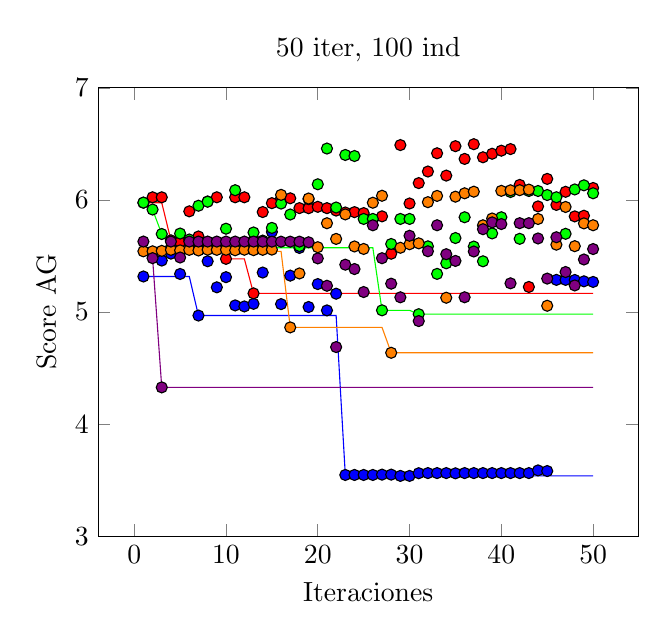
\begin{tikzpicture}
      \begin{axis}[
      title={50 iter, 100 ind},
      xlabel={Iteraciones},
      ylabel={Score AG},
      ymin=3,ymax=7]
      
      \addplot[color=blue] coordinates {(1,5.31716560765335)(6,5.31716560765334)(7,4.96862046326828)(22,4.96862046326828)(23,3.54640427951115)(28,3.54640427951115)(29,3.53811747918634)(30,3.53798681439415)(50,3.53798681439415)};
      \addplot[only marks, mark options={fill=blue}] coordinates {(1,5.317165607653349)(2,5.526088464188462)(3,5.4593567023661835)(4,5.521001298020508)(5,5.339665500924273)(6,5.623493379518466)(7,4.9686204632682855)(8,5.452989124766122)(9,5.2205154885890295)(10,5.3111027880187835)(11,5.059221727412204)(12,5.049985700067712)(13,5.073239449955616)(14,5.352273392909208)(15,5.7150789205196055)(16,5.070660532761057)(17,5.324866687388045)(18,5.5719614678738045)(19,5.04488605661705)(20,5.249458895328059)(21,5.014626446799102)(22,5.16360256226548)(23,3.5464042795111554)(24,3.5464042795111554)(25,3.5464042795111554)(26,3.5464042795111554)(27,3.549343077529984)(28,3.549343077529984)(29,3.538117479186345)(30,3.5379868143941584)(31,3.561963002998516)(32,3.5631146884487643)(33,3.5631146884487643)(34,3.5631146884487643)(35,3.560888430545689)(36,3.5631146884487643)(37,3.5631146884487643)(38,3.5631146884487643)(39,3.5631146884487643)(40,3.5631146884487643)(41,3.5631264030798415)(42,3.5631780155094814)(43,3.5631831504755485)(44,3.5870192783777406)(45,3.581215923469903)(46,5.286986110729754)(47,5.286986110729754)(48,5.286094625134464)(49,5.274060341559792)(50,5.2685510422215)};
      
      \addplot[color=red] coordinates {(1,5.97528837262042)(3,5.97528837262042)(4,5.63968096396759)(5,5.62521661010001)(9,5.62521661010001)(10,5.47444398334997)(12,5.47444398334997)(13,5.16656362051286)(50,5.16656362051286)};
      \addplot[only marks, mark options={fill=red}] coordinates {(1,5.975288372620428)(2,6.0237954127902995)(3,6.0237954127902995)(4,5.639680963967596)(5,5.625216610100011)(6,5.898362813556831)(7,5.674219772353009)(8,5.986147210677439)(9,6.0237954127902995)(10,5.474443983349973)(11,6.0237954127902995)(12,6.0237954127902995)(13,5.166563620512868)(14,5.892124722781776)(15,5.971477274163881)(16,6.013594589851077)(17,6.014792378740886)(18,5.927199869349108)(19,5.92635546953233)(20,5.938742898702474)(21,5.926845272313157)(22,5.905335867962531)(23,5.888061750002121)(24,5.891324815856076)(25,5.882629103829256)(26,5.825768961618586)(27,5.853759614315843)(28,5.520121550787666)(29,6.48965418399559)(30,5.968462629915473)(31,6.150357947361487)(32,6.25363778191767)(33,6.41648323265259)(34,6.2173339346509815)(35,6.479800712323088)(36,6.366177761402993)(37,6.497546764788726)(38,6.380800385816734)(39,6.412281373597008)(40,6.43955723991383)(41,6.453930687011264)(42,6.134278935928372)(43,5.22389454846507)(44,5.942545300394233)(45,6.187852564703526)(46,5.955919560258156)(47,6.072674998258606)(48,5.8533659516322265)(49,5.859207340857992)(50,6.106850063648894)};
      
      \addplot[color=green] coordinates {(1,5.97648738560558)(2,5.91441663097243)(3,5.69622538712708)(4,5.5754695897371)(8,5.5754695897371)(9,5.57389592247242)(26,5.57389592247242)(27,5.01525697418331)(30,5.01525697418331)(31,4.98072343998899)(50,4.98072343998899)};
      \addplot[only marks, mark options={fill=green}] coordinates {(1,5.976487385605589)(2,5.914416630972434)(3,5.696225387127081)(4,5.575469589737107)(5,5.70042336689882)(6,5.647289820658781)(7,5.9484805677203045)(8,5.984515418716362)(9,5.573895922472422)(10,5.743675472005052)(11,6.08700561551899)(12,5.618991351431977)(13,5.709795364818142)(14,5.637271839767401)(15,5.750755355620715)(16,5.967750014056639)(17,5.870273554736669)(18,5.589197419623724)(19,6.007097743768514)(20,6.13984690777907)(21,6.4587235816984485)(22,5.932773599610653)(23,6.401503897319305)(24,6.391966111271023)(25,5.8306487078687885)(26,5.8306487078687885)(27,5.015256974183311)(28,5.607103056573461)(29,5.8306487078687885)(30,5.8306487078687885)(31,4.980723439988992)(32,5.5861321474151975)(33,5.340419089212487)(34,5.434891909404775)(35,5.660225227314552)(36,5.845711320213284)(37,5.584193603123783)(38,5.45273586818372)(39,5.701541160839394)(40,5.845711320213284)(41,6.0708479977615415)(42,5.653225140969068)(43,6.079927997253662)(44,6.079927997253662)(45,6.043955114436508)(46,6.024232081044255)(47,5.69797691845686)(48,6.093741343112313)(49,6.130560141516949)(50,6.059674968160127)};
      
      \addplot[color=orange] coordinates{(1,5.54173118619805)(16,5.54173118619805)(17,4.86303668348638)(27,4.86303668348638)(28,4.63636394359056)(50,4.63636394359056)};
      \addplot[only marks, mark options={fill=orange}] coordinates {(1,5.541731186198051)(2,5.541731186198051)(3,5.545688519297611)(4,5.554775060697433)(5,5.549884179280587)(6,5.554775060697433)(7,5.549367506702051)(8,5.556305817991843)(9,5.554854598947674)(10,5.555470053923003)(11,5.551167308024191)(12,5.555842416091483)(13,5.552236961783379)(14,5.555019258034945)(15,5.556897391383615)(16,6.045408192912217)(17,4.8630366834863805)(18,5.344348233531942)(19,6.012699515333807)(20,5.578513134846146)(21,5.792320669216242)(22,5.652421005833398)(23,5.871115223951781)(24,5.585165076624916)(25,5.562865762074182)(26,5.975213896821525)(27,6.037361911489166)(28,4.6363639435905615)(29,5.5734287172774675)(30,5.604987335756016)(31,5.612957752789771)(32,5.980332184928363)(33,6.03616050396201)(34,5.127553476597928)(35,6.029280548500651)(36,6.0593766916540055)(37,6.073794336404768)(38,5.773970091684239)(39,5.834509330875364)(40,6.081283228417865)(41,6.0861277713741675)(42,6.087220695125776)(43,6.092444010890421)(44,5.830256176250252)(45,5.056056679222757)(46,5.601031347745641)(47,5.937513160188432)(48,5.587657351876355)(49,5.791053244081267)(50,5.774560830334639)};
      
      \addplot[color=violet] coordinates {(1,5.62872234265363)(2,5.48084527507771)(3,4.32775951328745)(50,4.32775951328745)};
      \addplot[only marks, mark options={fill=violet}] coordinates {(1,5.628722342653633)(2,5.480845275077714)(3,4.327759513287454)(4,5.628722342653633)(5,5.486652556962722)(6,5.628722342653633)(7,5.628722342653633)(8,5.628722342653633)(9,5.628722342653633)(10,5.628722342653633)(11,5.628722342653633)(12,5.628722342653633)(13,5.628722342653633)(14,5.628052941564771)(15,5.628052941564771)(16,5.628052941564771)(17,5.628052941564771)(18,5.628052941564771)(19,5.622476515725063)(20,5.478619575430889)(21,5.234296541345393)(22,4.687368824027697)(23,5.422407217766736)(24,5.3835556103069715)(25,5.17835758156074)(26,5.774110845071101)(27,5.480316206713727)(28,5.253027516118969)(29,5.131449862347445)(30,5.68059837496539)(31,4.919499466471914)(32,5.5423894539095055)(33,5.774279815607978)(34,5.516091333506565)(35,5.456156539170195)(36,5.131714030439232)(37,5.54022583924273)(38,5.739028189981615)(39,5.799937928486725)(40,5.78507475875881)(41,5.256211798934787)(42,5.792970293067738)(43,5.792970293067738)(44,5.656517671527621)(45,5.298409838058463)(46,5.667319034029117)(47,5.356909870171492)(48,5.237371667705103)(49,5.468747172394351)(50,5.5619025763218274)};
      
      \end{axis}
\end{tikzpicture}}
\end{subfigure}
% FIGURE 31
\begin{subfigure}[b]{0.43\textwidth}
\resizebox{\linewidth}{!}{
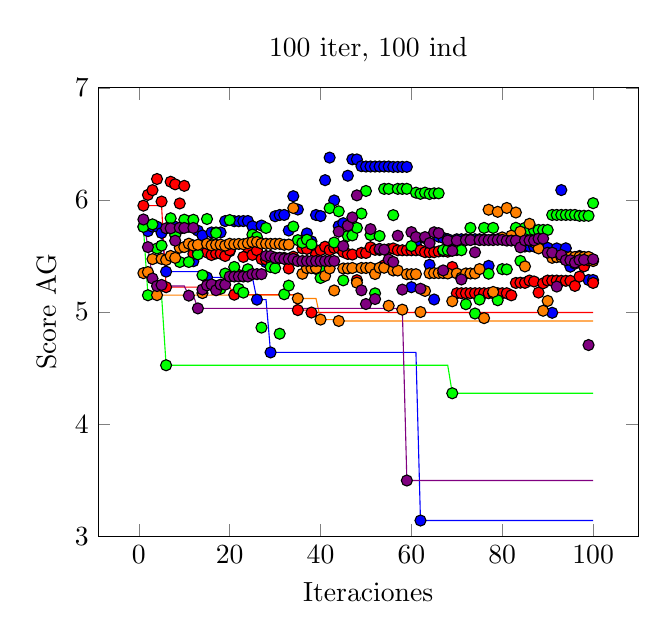
\begin{tikzpicture}
      \begin{axis}[
      title={100 iter, 100 ind},
      xlabel={Iteraciones},
      ylabel={Score AG},
      ymin=3,ymax=7]
      
      \addplot[color=blue] coordinates {(1,5.76183355527193)(2,5.72184130941125)(4,5.72184130941125)(5,5.70559547105243)(6,5.36066818793986)(14,5.36066818793986)(15,5.30910762677644)(25,5.30910762677644)(26,5.11047617084466)(28,5.11047617084466)(29,4.63959390196138)(61,4.63959390196138)(62,3.13989193983211)(100,3.13989193983211)};
      \addplot[only marks, mark options={fill=blue}] coordinates {(1,5.761833555271945)(2,5.721841309411252)(3,5.761833555271945)(4,5.761833555271945)(5,5.705595471052433)(6,5.3606681879398685)(7,5.7616147782092675)(8,5.7614543038299875)(9,5.741795250844181)(10,5.755653583299059)(11,5.7614543038299875)(12,5.453078272690885)(13,5.725677289956341)(14,5.682953506686077)(15,5.309107626776442)(16,5.709933150091032)(17,5.709933150091032)(18,5.709933150091032)(19,5.811528565199369)(20,5.542011838230901)(21,5.810452568644281)(22,5.810452568644281)(23,5.811528565199369)(24,5.812356269612233)(25,5.765010229538165)(26,5.110476170844668)(27,5.771785248535415)(28,5.443712509423756)(29,4.6395939019613825)(30,5.854634857427648)(31,5.865857207450562)(32,5.866242504728813)(33,5.7275317369923275)(34,6.033523275564649)(35,5.914658039905108)(36,5.641054605110663)(37,5.701476537256463)(38,5.630741160685778)(39,5.86578638017083)(40,5.856327845330769)(41,6.176567683639089)(42,6.377896882100589)(43,5.995549069806188)(44,5.766742510676822)(45,5.792581606552709)(46,6.216245266714344)(47,6.3622913918748925)(48,6.3617036484595335)(49,6.3012717735746975)(50,6.298231774898769)(51,6.298231774898769)(52,6.298231774898769)(53,6.298231774898769)(54,6.298231774898769)(55,6.298231774898769)(56,6.295013537349652)(57,6.295022748751631)(58,6.295163504871484)(59,6.295163504871484)(60,5.221596925840155)(61,5.602020151781252)(62,3.1398919398321157)(63,5.658421842432253)(64,5.421456084274825)(65,5.111915807486946)(66,5.672302422425117)(67,5.661817118220842)(68,5.6502176702955715)(69,5.61638611465804)(70,5.649294246760114)(71,5.6493023192894665)(72,5.649398492569084)(73,5.649414392975034)(74,5.649445205989411)(75,5.649512543757008)(76,5.647435797729991)(77,5.412213997182979)(78,5.648994043761704)(79,5.649290962799379)(80,5.6498141429442175)(81,5.650099913504862)(82,5.653248399519526)(83,5.645892999870697)(84,5.584841129280653)(85,5.585087391502442)(86,5.585244018828025)(87,5.585293924664941)(88,5.5852942469007125)(89,5.5827936671569525)(90,5.5729298888165895)(91,4.993440050964439)(92,5.567760376941006)(93,6.088137480584495)(94,5.568919434800059)(95,5.404739665179912)(96,5.431571495594541)(97,5.500051999089323)(98,5.4114158694150944)(99,5.2856973560073035)(100,5.2856973560073035)};
      
      \addplot[color=red] coordinates {(1,5.94909409205579)(5,5.94909409205579)(6,5.22171707433008)(20,5.22171707433008)(21,5.15467136376492)(34,5.15467136376492)(35,5.0170289037608)(37,5.0170289037608)(38,4.99555503543509)(100,4.99555503543509)};
      \addplot[only marks, mark options={fill=red}] coordinates {(1,5.949094092055795)(2,6.045406203976659)(3,6.087394120011508)(4,6.186913150131088)(5,5.985736836110368)(6,5.221717074330087)(7,6.1624098488704995)(8,6.139498572024981)(9,5.968811471242415)(10,6.125888885100372)(11,5.603510144863453)(12,5.518363110710353)(13,5.534222802495572)(14,5.591141302868287)(15,5.531700428175444)(16,5.50876638307461)(17,5.523172966874145)(18,5.52042946010326)(19,5.500107457383787)(20,5.550822059123915)(21,5.15467136376492)(22,5.331043933703126)(23,5.491607562482174)(24,5.576834405912672)(25,5.510018906256624)(26,5.55094473596492)(27,5.472628827330428)(28,5.468161650975989)(29,5.472278718122185)(30,5.483343617437533)(31,5.483359246832185)(32,5.483390464308581)(33,5.388398315078732)(34,5.493568059470105)(35,5.0170289037608)(36,5.567186548349333)(37,5.563462267333458)(38,4.995555035435095)(39,5.513755042480826)(40,5.552807247339432)(41,5.582732922405975)(42,5.552189306580507)(43,5.5719141914340815)(44,5.570682718615066)(45,5.53534070823279)(46,5.5182033621248365)(47,5.513085250038772)(48,5.284516736139553)(49,5.528069681804569)(50,5.526967119684273)(51,5.577860705729588)(52,5.554971034768412)(53,5.553928977910072)(54,5.416657698141032)(55,5.560477420392416)(56,5.567296630181516)(57,5.550963006196192)(58,5.550987020696161)(59,5.551043455474412)(60,5.551079680280548)(61,5.55109215448449)(62,5.5510928934727115)(63,5.53398559629756)(64,5.533985611574984)(65,5.533985972541113)(66,5.540860306435659)(67,5.543149136292119)(68,5.538288721078764)(69,5.401548956330108)(70,5.167723888449455)(71,5.167723888449455)(72,5.167723888449455)(73,5.167723888449455)(74,5.167723888449455)(75,5.167723888449455)(76,5.167723888449455)(77,5.167723888449455)(78,5.167723888449455)(79,5.167723888449455)(80,5.167723888449455)(81,5.167723888449455)(82,5.148909151216138)(83,5.259429813487645)(84,5.262173802647504)(85,5.260112944514443)(86,5.280905865490096)(87,5.272328643794981)(88,5.173595689961083)(89,5.256338274748991)(90,5.280905865490096)(91,5.280678872081434)(92,5.2808107469708965)(93,5.27872543911503)(94,5.278343693781894)(95,5.27864417435854)(96,5.233110550514865)(97,5.31578479073887)(98,5.407970443208814)(99,5.460644347131443)(100,5.25969866435715)};
      
      \addplot[color=green] coordinates {(1,5.75977478229486)(2,5.14977175037173)(5,5.14977175037173)(6,4.52512755122917)(68,4.52512755122917)(69,4.27532197953086)(100,4.27532197953086)};
      \addplot[only marks, mark options={fill=green}] coordinates {(1,5.759774782294868)(2,5.149771750371739)(3,5.782216944930093)(4,5.5673620175398835)(5,5.593086293319294)(6,4.5251275512291755)(7,5.83676798121374)(8,5.687592234522896)(9,5.446363666094714)(10,5.824130095318273)(11,5.446445434370169)(12,5.823129026809612)(13,5.514626116659199)(14,5.329016637215453)(15,5.83005769580724)(16,5.6070128404413975)(17,5.704448307760762)(18,5.207470509437298)(19,5.3434675174631785)(20,5.820738314120356)(21,5.4022632832117985)(22,5.206548111514724)(23,5.173374790843756)(24,5.381597158325386)(25,5.6909874016760895)(26,5.668242846839849)(27,4.861117113963259)(28,5.750094270765166)(29,5.400959224448932)(30,5.39161926013332)(31,4.806505813760589)(32,5.158303572624334)(33,5.23577395036892)(34,5.7626652906493625)(35,5.641448868428301)(36,5.617520450147532)(37,5.645452335918934)(38,5.603712196633873)(39,5.384918026445664)(40,5.3039444258647475)(41,5.375738673511343)(42,5.926832888584842)(43,5.620150059223219)(44,5.8985612623487285)(45,5.282672254197603)(46,5.678783944779636)(47,5.683804809586075)(48,5.751230832157503)(49,5.878511406974077)(50,6.08011227046671)(51,5.687297484860066)(52,5.166707755972168)(53,5.678436416639471)(54,6.098922370284322)(55,6.098922370284322)(56,5.864596557332897)(57,6.098922370284322)(58,6.098922370284322)(59,6.099180067537872)(60,5.588645086885489)(61,6.065160672119223)(62,6.054722977527225)(63,6.065160672119223)(64,6.053368956589235)(65,6.058953794605747)(66,6.058953794605747)(67,5.553293203027788)(68,5.553293203027788)(69,4.275321979530866)(70,5.553293203027788)(71,5.5516157756185365)(72,5.069797228121256)(73,5.750779595078901)(74,4.986913713341241)(75,5.110935026911345)(76,5.750779595078901)(77,5.341973719758853)(78,5.750779595078901)(79,5.105079486727984)(80,5.382806156521076)(81,5.3805795963801355)(82,5.642737799695024)(83,5.751516392050274)(84,5.455589263366687)(85,5.75121917090139)(86,5.732372218893852)(87,5.732372218893852)(88,5.732372218893852)(89,5.732372218893852)(90,5.732372218893852)(91,5.866379155201184)(92,5.866379155201184)(93,5.866379155201184)(94,5.866379155201184)(95,5.866379155201184)(96,5.866379155201184)(97,5.858674489722834)(98,5.858674489722834)(99,5.858674489722834)(100,5.97150706650781)};
      
      \addplot[color=orange] coordinates{(1,5.34701018868541)(3,5.34701018868541)(4,5.15090764367699)(34,5.15090764367699)(35,5.12116090196805)(39,5.12116090196805)(40,4.93258741102162)(43,4.93258741102162)(44,4.92034398916437)(100,4.92034398916437)};
      \addplot[only marks, mark options={fill=orange}] coordinates {(1,5.347010188685415)(2,5.3565705957446905)(3,5.472284833001991)(4,5.150907643676993)(5,5.4741413893171185)(6,5.464568941874449)(7,5.500641383322389)(8,5.483146583561877)(9,5.573798514146412)(10,5.579895815075542)(11,5.609904900335201)(12,5.59311399649806)(13,5.600218505976873)(14,5.168960983278758)(15,5.609077935589799)(16,5.594744643394112)(17,5.600476239260816)(18,5.601517446026836)(19,5.592309759107097)(20,5.609250019500726)(21,5.604226322627028)(22,5.607741414972358)(23,5.604660523148818)(24,5.61435130071381)(25,5.624725659070741)(26,5.624875916499529)(27,5.611036853047628)(28,5.609167531278428)(29,5.608173632889516)(30,5.608390766672997)(31,5.608641496094082)(32,5.600067276228151)(33,5.601829345023291)(34,5.927964787727746)(35,5.121160901968054)(36,5.341022566601737)(37,5.391748969634267)(38,5.391748969634267)(39,5.391748969634267)(40,4.932587411021629)(41,5.322470619955591)(42,5.388662954675978)(43,5.192175616508683)(44,4.920343989164374)(45,5.388662954675978)(46,5.388662954675978)(47,5.392856317653413)(48,5.261341156360089)(49,5.392935047884455)(50,5.392935047884455)(51,5.394589230696247)(52,5.339290472977453)(53,5.395048101751596)(54,5.395048101751596)(55,5.056391988214428)(56,5.370740363723188)(57,5.370740363723188)(58,5.02133692617108)(59,5.337490668640694)(60,5.337490668640694)(61,5.337490668640694)(62,4.999918277973344)(63,5.188332214467499)(64,5.345922172048826)(65,5.347664645873261)(66,5.347664645873261)(67,5.347664645873261)(68,5.344193731719001)(69,5.0962765617393835)(70,5.344193731719001)(71,5.306153338625974)(72,5.344193731719001)(73,5.344193731719001)(74,5.344193731719001)(75,5.383161205549941)(76,4.945680855477834)(77,5.912899547117709)(78,5.179154586845546)(79,5.8942097046768325)(80,5.665826924012788)(81,5.928507827686201)(82,5.681316493451102)(83,5.887982245150572)(84,5.7174564719412)(85,5.407042813397199)(86,5.787069534063296)(87,5.622559396837499)(88,5.567645090246604)(89,5.011555420172087)(90,5.099195949722177)(91,5.483630038557348)(92,5.489800146748324)(93,5.489800146748324)(94,5.491720496930145)(95,5.491720496930145)(96,5.491720496930145)(97,5.491720496930145)(98,5.491720496930145)(99,5.491720496930145)(100,5.4548415876265794)};
      
      \addplot[color=violet] coordinates {(1,5.82576995149594)(2,5.57933882069317)(3,5.29932645242455)(4,5.23194962155138)(10,5.23194962155138)(11,5.14636053042995)(12,5.14636053042995)(13,5.03244778251099)(58,5.03244778251099)(59,3.49686045534989)(100,3.49686045534989)};
      \addplot[only marks, mark options={fill=violet}] coordinates {(1,5.8257699514959445)(2,5.579338820693172)(3,5.29932645242455)(4,5.231949621551388)(5,5.242078937059539)(6,5.746764216768215)(7,5.746621401590604)(8,5.63648019172817)(9,5.751883897307964)(10,5.750554659150906)(11,5.146360530429956)(12,5.750554659150906)(13,5.03244778251099)(14,5.200970129287104)(15,5.237553163033519)(16,5.246074857715689)(17,5.19437554927507)(18,5.2443765727810225)(19,5.2443765727810225)(20,5.316978646409037)(21,5.316978646409037)(22,5.316978646409037)(23,5.316978646409037)(24,5.316978646409037)(25,5.338069440455346)(26,5.338069440455346)(27,5.338069440455346)(28,5.499883099990122)(29,5.499883099990122)(30,5.483103225531586)(31,5.483103225531586)(32,5.47394928502705)(33,5.47394928502705)(34,5.47394928502705)(35,5.454868282340808)(36,5.454868282340808)(37,5.454868282340808)(38,5.454904020784082)(39,5.454904020784082)(40,5.454904020784082)(41,5.454904020784082)(42,5.454904020784082)(43,5.454904020784082)(44,5.717508426728006)(45,5.588134700070725)(46,5.77088437656664)(47,5.844255850054502)(48,6.040916505782674)(49,5.193645429418332)(50,5.071490613356103)(51,5.739551267106736)(52,5.115929612246148)(53,5.5633306223164665)(54,5.556891299178117)(55,5.468965908085554)(56,5.446959052169547)(57,5.680840795917539)(58,5.200176137700925)(59,3.4968604553498928)(60,5.712787979990743)(61,5.668709963720855)(62,5.207910513613788)(63,5.668709629400512)(64,5.6148954900543595)(65,5.711349088656357)(66,5.703630243585657)(67,5.371276582058775)(68,5.6383156754254)(69,5.5459184492844145)(70,5.63879929453644)(71,5.290768116149039)(72,5.641998743423207)(73,5.641998743423207)(74,5.532827261886329)(75,5.641998743423207)(76,5.642187610809447)(77,5.642187610809447)(78,5.642187610809447)(79,5.644606449276063)(80,5.644606449276063)(81,5.6374782303891156)(82,5.6374782303891156)(83,5.6374782303891156)(84,5.577011826990621)(85,5.638628265016514)(86,5.638628265016514)(87,5.638628265016514)(88,5.655226686630523)(89,5.655226686630523)(90,5.529576598268735)(91,5.529576598268735)(92,5.2273622785465115)(93,5.508895492373334)(94,5.462278352134817)(95,5.462194335791914)(96,5.441213573092291)(97,5.464153461363143)(98,5.465782495413921)(99,4.70553632268069)(100,5.470683029131118)};
      
      \end{axis}
\end{tikzpicture}}
\end{subfigure}
\newline
\centering
% FIGURE 32
\begin{subfigure}[b]{0.43\textwidth}
\resizebox{\linewidth}{!}{
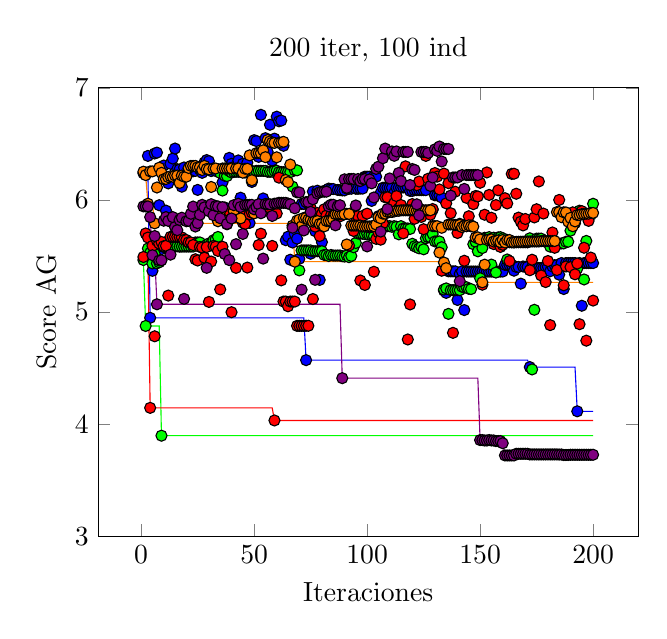
\begin{tikzpicture}
      \begin{axis}[
      title={200 iter, 100 ind},
      xlabel={Iteraciones},
      ylabel={Score AG},
      ymin=3,ymax=7]
      
      \addplot[color=blue] coordinates {(1,6.23848498843278)(3,6.23848498843278)(4,4.94826632575501)(72,4.94826632575501)(73,4.57079330988966)(171,4.57079330988966)(172,4.50886494632023)(192,4.50886494632023)(193,4.11428234593617)(200,4.11428234593617)};
      \addplot[only marks, mark options={fill=blue}] coordinates {(1,6.238484988432786)(2,6.244318984470536)(3,6.393084607926424)(4,4.948266325755011)(5,5.367532321899503)(6,6.414569854849189)(7,6.422319837365886)(8,5.952914670676327)(9,5.5605808299922295)(10,6.306960373367606)(11,5.904845346971847)(12,6.14775934150437)(13,6.322744579785917)(14,6.36910921929929)(15,6.458754335922766)(16,6.273847583234749)(17,6.271060760947624)(18,6.118049282398281)(19,6.2899087294120015)(20,6.2183145540642055)(21,6.277710773743623)(22,6.2570543774937954)(23,6.255842715516328)(24,6.2592649790464225)(25,6.089606191872059)(26,6.269794666079764)(27,6.241962390323907)(28,6.334268073806202)(29,6.355849522814083)(30,6.346227103748064)(31,6.257557810560741)(32,6.281008464567148)(33,6.258486453405115)(34,6.274629548405388)(35,6.2669126087988385)(36,6.156548625767426)(37,5.933270019877426)(38,5.846692255399787)(39,6.375366908053927)(40,6.322445083780328)(41,6.294006586667826)(42,6.292089517748198)(43,6.352774448473315)(44,6.020175436292681)(45,6.322947285087236)(46,6.283320148589491)(47,6.333073743001853)(48,5.795207748774223)(49,6.160629834642342)(50,6.533701539612258)(51,6.525673997253542)(52,6.384642380231478)(53,6.759459260412519)(54,6.013565244506081)(55,6.551320589524384)(56,6.42845356607656)(57,6.671097510904488)(58,6.351184592811958)(59,6.547082575513846)(60,6.743202240118466)(61,6.70188702697048)(62,6.708421903017744)(63,6.483306805987717)(64,5.641165696216944)(65,5.672869162570363)(66,5.466537316766088)(67,5.620191346302336)(68,5.696218134620748)(69,5.65496838441622)(70,5.474875065571945)(71,5.964495486806461)(72,5.964495486806461)(73,4.57079330988966)(74,5.964495486806461)(75,5.520043376488557)(76,6.075176000538193)(77,5.7219267664162725)(78,6.082862049177456)(79,5.286692729226376)(80,5.623537620543211)(81,5.869051052566984)(82,6.089497552269406)(83,6.101459453577154)(84,6.09823428702229)(85,6.097561632703202)(86,5.833360954493548)(87,6.0894168534271715)(88,6.087737448872101)(89,6.085398269054627)(90,6.085339721458173)(91,6.100205037836348)(92,6.100205037836348)(93,6.100205037836348)(94,5.887488886070969)(95,6.0998939106196115)(96,6.0998939106196115)(97,6.101276744115413)(98,6.101276744115413)(99,6.2079105867945135)(100,6.2079105867945135)(101,6.2079105867945135)(102,5.991665704295201)(103,6.2079105867945135)(104,6.2079105867945135)(105,5.855269712465564)(106,6.062964679951633)(107,6.109284406127395)(108,6.109284406127395)(109,6.109284406127395)(110,6.109284406127395)(111,6.109284406127395)(112,6.062189913845868)(113,6.109284406127395)(114,6.109284406127395)(115,6.109284406127395)(116,6.112005185792762)(117,6.112005185792762)(118,6.112005185792762)(119,6.080472300437952)(120,6.080472300437952)(121,6.087712962917733)(122,6.08763306158505)(123,6.087658458670304)(124,6.087627087148864)(125,6.087712962917733)(126,6.087712962917733)(127,5.677113471568524)(128,5.897381951124787)(129,5.91172330516926)(130,6.041133803291496)(131,6.041133803291496)(132,6.041133803291496)(133,6.02157420664311)(134,5.191080900679598)(135,5.170997104065691)(136,5.362962811738177)(137,5.362962811738177)(138,5.362953794020128)(139,5.362953794020128)(140,5.10774321226545)(141,5.339889814339133)(142,5.362953794020128)(143,5.017590898275847)(144,5.361304270414172)(145,5.361304270414172)(146,5.361304270414172)(147,5.361304270414172)(148,5.361304270414172)(149,5.361304270414172)(150,5.361304270414172)(151,5.361304270414172)(152,5.361304270414172)(153,5.361304270414172)(154,5.360671669412426)(155,5.361304270414172)(156,5.361304270414172)(157,5.361304270414172)(158,5.361304270414172)(159,5.361304270414172)(160,5.361304270414172)(161,5.42100430229625)(162,5.4203197930204405)(163,5.4203197930204405)(164,5.4203197930204405)(165,5.36881637067701)(166,5.402376630305198)(167,5.402376630305198)(168,5.25339236884028)(169,5.406480716450968)(170,5.4032937377100865)(171,5.402943555355381)(172,4.508864946320236)(173,5.4049367310006895)(174,5.393074335369882)(175,5.39308481029668)(176,5.393096061945943)(177,5.393108366267915)(178,5.393323146195357)(179,5.401734786120142)(180,5.4049147738402255)(181,5.363689014425535)(182,5.406742006348298)(183,5.418000520201343)(184,5.418000520201343)(185,5.333084196466322)(186,5.437052311507912)(187,5.205481482728182)(188,5.437052311507912)(189,5.437052311507912)(190,5.437052311507912)(191,5.437052311507912)(192,5.437052311507912)(193,4.114282345936173)(194,5.437020898997586)(195,5.056127173052153)(196,5.437052311507912)(197,5.437052311507912)(198,5.437052311507912)(199,5.437052311507912)(200,5.437052311507913)};
      
      \addplot[color=green] coordinates {(1,5.46433054322024)(2,4.87585154084038)(8,4.87585154084038)(9,3.89672367936541)(200,3.89672367936541)};
      \addplot[only marks, mark options={fill=green}] coordinates {(1,5.464330543220247)(2,4.875851540840383)(3,5.567169080268749)(4,5.52848869434788)(5,5.43391949910973)(6,5.517583798854341)(7,5.434676173518988)(8,5.443553702453384)(9,3.8967236793654134)(10,5.579704011920585)(11,5.625312492134498)(12,5.581622250191295)(13,5.6198103713169205)(14,5.614033974962906)(15,5.585593921877248)(16,5.585916029573559)(17,5.58317351762414)(18,5.58371357800379)(19,5.583821067398899)(20,5.584032708171954)(21,5.584050276541949)(22,5.58405057978283)(23,5.584051060571053)(24,5.6207817921046255)(25,5.620781796358871)(26,5.621019072199083)(27,5.5759245769028105)(28,5.578157067999985)(29,5.598952214284017)(30,5.61220074007789)(31,5.6125056781897005)(32,5.640792962851931)(33,5.648787682827555)(34,5.670157282385767)(35,6.240793421195702)(36,6.083816372768621)(37,6.215936518046535)(38,6.212674003116886)(39,6.258153426450314)(40,6.2450134399003225)(41,6.250388598985705)(42,6.251251502804479)(43,6.251573655024288)(44,6.252259650556664)(45,6.252477497715727)(46,6.244766341077886)(47,6.259581684353321)(48,6.253310441420468)(49,6.259581684353321)(50,6.251111773832092)(51,6.259581684353321)(52,6.259581684353321)(53,6.259581684353321)(54,6.259581684353321)(55,6.259581684353321)(56,6.251392871454096)(57,6.251355231974011)(58,6.2522639074571025)(59,6.259581684353321)(60,6.261090112951537)(61,6.248741659845128)(62,6.24915051831748)(63,6.247749150798311)(64,6.248168174280727)(65,6.249066726096814)(66,6.247339802037264)(67,6.1191944743544155)(68,6.2642687083429465)(69,6.2642687083429465)(70,5.371529052371578)(71,5.549719410660428)(72,5.549719410660428)(73,5.549719410660428)(74,5.549719410660428)(75,5.549719410660428)(76,5.542309252034982)(77,5.542309252034982)(78,5.542309252034982)(79,5.542309252034982)(80,5.542309252034982)(81,5.50969835428913)(82,5.50969835428913)(83,5.5000326414507335)(84,5.5089838408659215)(85,5.504239872661023)(86,5.503801302456793)(87,5.504483534905453)(88,5.504483534905453)(89,5.498069732982287)(90,5.4949322847512345)(91,5.504907824150559)(92,5.489672016405207)(93,5.500523864101098)(94,5.578132944426455)(95,5.616322696213355)(96,5.699873768422748)(97,5.699873768422748)(98,5.698397288116185)(99,5.695292584986449)(100,5.699873768422748)(101,5.68852325813657)(102,5.68852325813657)(103,5.677837967546711)(104,5.766031725812292)(105,5.766031725812292)(106,5.766031725812292)(107,5.766031725812292)(108,5.7660381224590065)(109,5.7660381224590065)(110,5.7660381224590065)(111,5.760185474314689)(112,5.7660381224590065)(113,5.760697650292016)(114,5.693195435081037)(115,5.766255927916836)(116,5.746071990479269)(117,5.746130158669692)(118,5.745428702360561)(119,5.740829582822873)(120,5.608928086963315)(121,5.586918387972737)(122,5.5781892186493955)(123,5.568296104829969)(124,5.580874095803727)(125,5.5595853577587935)(126,5.6583024447491805)(127,5.667258999085577)(128,5.667232332713943)(129,5.696406032831184)(130,5.630021530237585)(131,5.630021530237585)(132,5.630021530237585)(133,5.57813075706644)(134,5.201054452344147)(135,5.210851396550602)(136,4.983581888213804)(137,5.195187043503138)(138,5.195187043503138)(139,5.195187043503138)(140,5.195187043503138)(141,5.195187043503138)(142,5.226034076411418)(143,5.218439656659889)(144,5.221478289905672)(145,5.207212380212731)(146,5.2047625362743855)(147,5.605087726824475)(148,5.626959688508446)(149,5.541630026426468)(150,5.301301204926887)(151,5.570898499802213)(152,5.662585307891115)(153,5.661399921830586)(154,5.668378578542132)(155,5.42314517676207)(156,5.66323909667387)(157,5.3523458872476946)(158,5.666116688922859)(159,5.667825700412893)(160,5.658169703594293)(161,5.6360377746890515)(162,5.469001892032585)(163,5.622703165305392)(164,5.622703165305392)(165,5.622703165305392)(166,5.622703165305392)(167,5.622703165305392)(168,5.622703165305392)(169,5.622703165305392)(170,5.622703165305392)(171,5.622703165305392)(172,5.658042609648978)(173,4.487905882384108)(174,5.01986022212145)(175,5.655021481838654)(176,5.655021481838654)(177,5.655021481838654)(178,5.636470275703244)(179,5.626924251130518)(180,5.626924251130518)(181,5.583287158090698)(182,5.621607873397939)(183,5.608943027497331)(184,5.610014845007088)(185,5.610066975634186)(186,5.6121548168358695)(187,5.612292991645256)(188,5.626880426369775)(189,5.6275473800837625)(190,5.725343180954798)(191,5.8301112710667855)(192,5.792337344686034)(193,5.387240310514375)(194,5.904529077424312)(195,5.873279518142909)(196,5.290604425144258)(197,5.6343491662772545)(198,5.876236794475557)(199,5.865887718783638)(200,5.965921997803036)};
      
      \addplot[color=red] coordinates {(1,5.49111748653079)(3,5.49111748653079)(4,4.14507904643707)(58,4.14507904643707)(59,4.03273303529719)(200,4.03273303529719)};
      \addplot[only marks, mark options={fill=red}] coordinates {(1,5.4911174865307935)(2,5.70120379859617)(3,5.6644004697840575)(4,4.14507904643707)(5,5.590452762407983)(6,4.783577675615681)(7,5.6355337933415255)(8,5.611648399905151)(9,5.625048323836301)(10,5.587847608545836)(11,5.590877773335446)(12,5.146887483790975)(13,5.670992572247729)(14,5.670992572247729)(15,5.670992572247729)(16,5.670992572247729)(17,5.670992572247729)(18,5.6664802918758586)(19,5.643834692235195)(20,5.64303890799304)(21,5.62210982771019)(22,5.621018486628179)(23,5.597962651308896)(24,5.470890205616866)(25,5.459618484636437)(26,5.581239963134782)(27,5.575814934364571)(28,5.485058552048342)(29,5.5797013136562645)(30,5.090266830391867)(31,5.450537353601853)(32,5.589495205540027)(33,5.583261166361413)(34,5.545236945099603)(35,5.201459750694382)(36,5.582893879108711)(37,5.878292126061022)(38,5.782892694374629)(39,5.898719972131266)(40,4.99845860339411)(41,5.902103790270786)(42,5.393986756384809)(43,5.875976878479796)(44,5.875976878479796)(45,5.797147398260424)(46,5.786109587970403)(47,5.39661525575813)(48,5.8723904644851554)(49,5.8873736666092285)(50,5.889123788124629)(51,5.88918829097693)(52,5.597766054019912)(53,5.699273895631535)(54,5.905815357093557)(55,5.907085000398956)(56,5.909770475061025)(57,5.9302383928876505)(58,5.589913370475881)(59,4.032733035297195)(60,5.8789756639415645)(61,6.198885076161601)(62,5.282555253590996)(63,5.093475886914651)(64,5.093475886914651)(65,5.051306894922146)(66,5.093475886914651)(67,5.0933052106918755)(68,5.0933052106918755)(69,4.876593027002097)(70,4.876593027002097)(71,4.876593027002097)(72,4.876593027002097)(73,4.8773862427208545)(74,4.8773862427208545)(75,5.931476346129733)(76,5.116021466662531)(77,5.761613909808267)(78,5.883142199815659)(79,5.677913052430204)(80,5.875719220330426)(81,5.91690962521227)(82,5.861383607398777)(83,5.813480935046968)(84,5.862561007216824)(85,5.852054370863768)(86,5.866851759014298)(87,5.866855276036918)(88,5.853670776590577)(89,5.876756199177466)(90,5.875262135303929)(91,5.875956959003912)(92,5.5929272430803625)(93,5.881777377390502)(94,5.72324244635786)(95,5.8539712920183264)(96,5.8559897977096185)(97,5.281519418863565)(98,5.857000596226479)(99,5.241603210609229)(100,5.877967558447095)(101,5.754266075020827)(102,5.75949089763743)(103,5.359289996825256)(104,5.652645717218933)(105,5.709637522277905)(106,5.645514380593887)(107,5.792099511552813)(108,6.023358509616806)(109,6.023358509616806)(110,5.896277312057249)(111,5.9429833354339845)(112,5.971761773795062)(113,6.034547309193552)(114,5.9226601455620935)(115,5.9548000637839404)(116,5.701808890413599)(117,6.29990711836102)(118,4.755109875031998)(119,5.0678118418279965)(120,5.963138340790742)(121,5.8321847017252075)(122,6.13204213643087)(123,6.164335371484263)(124,5.8486495579303455)(125,5.738783413151232)(126,6.393268989955299)(127,6.189334395677875)(128,5.867812976562871)(129,5.918874967578561)(130,6.239997018613211)(131,6.208313247254045)(132,6.093605037656643)(133,5.368553118305323)(134,6.235025123163683)(135,5.969372830495604)(136,6.150040894058453)(137,5.881683410555603)(138,4.814345084603382)(139,6.07333273251237)(140,5.7051247034354455)(141,5.787245392401303)(142,5.758355493536135)(143,5.45756398330915)(144,6.018470218520791)(145,5.854734251410047)(146,5.77245004445912)(147,5.962771070296167)(148,6.035335695447751)(149,6.0311453483745785)(150,6.153107666045115)(151,5.24361980945657)(152,5.868173237605937)(153,6.2455855092683334)(154,6.044875616986275)(155,5.841398840585892)(156,5.606157071664381)(157,5.954476045206885)(158,6.086344676460552)(159,5.58106924111188)(160,5.599731078429231)(161,6.015693113977573)(162,5.968904601472182)(163,5.454822658890928)(164,6.232632185522332)(165,6.234198717547017)(166,6.0554775068539)(167,5.842486737651473)(168,5.806291720523572)(169,5.772915042449791)(170,5.830230871602252)(171,5.623094905876556)(172,5.372888363578834)(173,5.466769318345497)(174,5.844136682728719)(175,5.9172015113514895)(176,6.164978343579676)(177,5.326201282087036)(178,5.878499492489924)(179,5.267435685015203)(180,5.455130805469657)(181,4.88337939864045)(182,5.709889774694135)(183,5.573093022513008)(184,5.3748058383834705)(185,6.000230580153442)(186,5.8592815068448445)(187,5.2386304329229585)(188,5.4066359960068455)(189,5.818608783764151)(190,5.400395601072365)(191,5.889423034485288)(192,5.336566427802837)(193,5.432576969538186)(194,4.891448942812179)(195,5.9002030198963435)(196,5.5735443314640865)(197,4.744452966011224)(198,5.813421457791698)(199,5.48591751792744)(200,5.102155416143097)};
      
      \addplot[color=orange] coordinates {(1,6.25207345334476)(2,6.22182283591779)(3,5.9665012628219)(5,5.9665012628219)(6,5.79129942832329)(66,5.79129942832329)(67,5.77080833518449)(68,5.44948662728703)(133,5.44948662728703)(134,5.44193009482722)(135,5.39166213550047)(150,5.39166213550047)(151,5.26509087914446)(200,5.26509087914446)};
      \addplot[only marks, mark options={fill=orange}] coordinates {(1,6.2520734533447655)(2,6.22182283591779)(3,5.966501262821907)(4,6.254344038797331)(5,6.254850886548603)(6,5.791299428323297)(7,6.111163675437458)(8,6.287704512053109)(9,6.241901417091376)(10,6.184938131847037)(11,6.187149321879232)(12,6.203528228010048)(13,6.211576351991779)(14,6.207320289296099)(15,6.217765066975265)(16,6.217734676868334)(17,6.151344240310836)(18,6.217412953675913)(19,6.208780115232534)(20,6.207333399334334)(21,6.285503578416383)(22,6.303950306723524)(23,6.303950306723524)(24,6.303950306723524)(25,6.291646004736608)(26,6.290208894939388)(27,6.267341424988322)(28,6.303950306723524)(29,6.277017457017576)(30,6.2733174783629755)(31,6.1157074112337115)(32,6.280702278129672)(33,6.280702278129672)(34,5.810025838324302)(35,5.901216399160959)(36,6.280702278129672)(37,6.280702278129672)(38,6.280702278129672)(39,6.280702278129672)(40,6.280702278129672)(41,5.900580301420593)(42,6.280702278129672)(43,6.280887141716414)(44,5.835640355211674)(45,6.243284405446957)(46,6.278369390469046)(47,6.27854807486914)(48,6.39811897973642)(49,6.176275448190157)(50,5.880798392645877)(51,6.41763755823896)(52,6.41763755823896)(53,6.41763755823896)(54,6.442892282924506)(55,6.381790745767505)(56,6.534916931142911)(57,6.52233201568038)(58,6.5123333363789015)(59,6.508740666072495)(60,6.380524743802209)(61,6.509991502666654)(62,6.512099066185007)(63,6.518383905308324)(64,6.178611526376088)(65,6.159344706988591)(66,6.316123872949961)(67,5.770808335184496)(68,5.4494866272870315)(69,5.816084411183239)(70,5.824043155733914)(71,5.764688891440299)(72,5.839904660541329)(73,5.839904660541329)(74,5.824765146298189)(75,5.8235744549197594)(76,5.806378762981115)(77,5.811138890173867)(78,5.811507057679626)(79,5.786393304206139)(80,5.7868128508016206)(81,5.7640237189221395)(82,5.812524857360155)(83,5.813598643599869)(84,5.813726324666826)(85,5.82367325228134)(86,5.872405739688097)(87,5.872405739688097)(88,5.872405739688097)(89,5.872405739688097)(90,5.872405739688097)(91,5.602740906972773)(92,5.874815687733226)(93,5.771603204868187)(94,5.771603204868187)(95,5.771603204868187)(96,5.771603204868187)(97,5.771663816015284)(98,5.76258542481467)(99,5.762663427529644)(100,5.76295451102612)(101,5.764140620248412)(102,5.76431913701607)(103,5.765952514466443)(104,5.780591907004887)(105,5.844882425890237)(106,5.837002317641128)(107,5.8778353783962185)(108,5.8778353783962185)(109,5.893075480754137)(110,5.893075480754137)(111,5.893075480754137)(112,5.897290691990772)(113,5.903076760677618)(114,5.903076760677618)(115,5.9075112261750355)(116,5.9075112261750355)(117,5.9075112261750355)(118,5.9075112261750355)(119,5.9075112261750355)(120,5.9075112261750355)(121,5.9075112261750355)(122,5.9075112261750355)(123,5.9075112261750355)(124,5.9075112261750355)(125,5.9075112261750355)(126,5.9075112261750355)(127,5.9075112261750355)(128,5.9075112261750355)(129,5.766322735151806)(130,5.766322735151806)(131,5.766322735151806)(132,5.530602376895525)(133,5.751699894344011)(134,5.441930094827223)(135,5.391662135500479)(136,5.781309001051129)(137,5.781309001051129)(138,5.781309001051129)(139,5.7771914922664855)(140,5.7771914922664855)(141,5.7771914922664855)(142,5.758838064855802)(143,5.768136276578213)(144,5.765420280131108)(145,5.773733253595635)(146,5.764269669673546)(147,5.762261837849545)(148,5.665345200006781)(149,5.666448027516818)(150,5.647930701680398)(151,5.265090879144462)(152,5.422641470163454)(153,5.643717943271746)(154,5.648483328384543)(155,5.648888189696058)(156,5.629697205235083)(157,5.637034494335463)(158,5.63835940761025)(159,5.6228489240259565)(160,5.642637980809532)(161,5.620655469406452)(162,5.642637980809532)(163,5.642637980809532)(164,5.622756831904211)(165,5.6210798324423585)(166,5.625925253357858)(167,5.626871925928615)(168,5.626999806368189)(169,5.627295136543692)(170,5.629352640550974)(171,5.629718910493598)(172,5.629816200410405)(173,5.629832900022391)(174,5.629833666005752)(175,5.629833921502804)(176,5.629833946379428)(177,5.632630767999046)(178,5.633189089772129)(179,5.6332536759196445)(180,5.633313082219807)(181,5.633381970788559)(182,5.633388047050774)(183,5.6334086248394115)(184,5.891668685802356)(185,5.891739747763294)(186,5.846392326877194)(187,5.889885242585937)(188,5.888653345150574)(189,5.806258245640258)(190,5.8397582954520555)(191,5.765211273624764)(192,5.808896720579822)(193,5.865411524632607)(194,5.865652583026531)(195,5.873529474515796)(196,5.8749427929848945)(197,5.877711227383584)(198,5.8777707373355925)(199,5.884336958664424)(200,5.884435894696505)};
      
      \addplot[color=violet] coordinates {(1,5.9426816914609)(3,5.9426816914609)(4,5.84681865337842)(5,5.50704648036729)(6,5.50704648036729)(7,5.06924914726654)(88,5.06924914726654)(89,4.40999327494372)(149,4.40999327494372)(150,3.85755707157541)(151,3.85755707157541)(152,3.85378836811247)(156,3.85378836811247)(157,3.84852358587115)(159,3.84852358587115)(160,3.82961024221691)(161,3.72052665732639)(200,3.72052665732639)};
      \addplot[only marks, mark options={fill=violet}] coordinates {(1,5.942681691460903)(2,5.942681691460903)(3,5.942681691460903)(4,5.846818653378428)(5,5.507046480367292)(6,5.6780033647133)(7,5.069249147266541)(8,5.459930515746331)(9,5.4618066903848845)(10,5.8146716475851274)(11,5.846960326710607)(12,5.813470789100554)(13,5.51204746088616)(14,5.846960326710607)(15,5.758187610145397)(16,5.730551490976016)(17,5.821622294688258)(18,5.841465405292438)(19,5.117550466757621)(20,5.810201370809744)(21,5.814122334163258)(22,5.877016134480305)(23,5.941052410686634)(24,5.762823900837661)(25,5.793374420010551)(26,5.867817560157906)(27,5.956411055507312)(28,5.933787340860318)(29,5.394385802704717)(30,5.899774812212897)(31,5.962262336902945)(32,5.8638748199769)(33,5.945793237463932)(34,5.942680551185072)(35,5.836426045533856)(36,5.935894423418915)(37,5.517604159286504)(38,5.786624841631999)(39,5.463272571115146)(40,5.8347958027665365)(41,5.95354127577083)(42,5.605549853087833)(43,5.966180000269626)(44,5.937604368698052)(45,5.696883516390814)(46,5.954513088397772)(47,5.9558475378530735)(48,5.95606895012024)(49,5.956216165512275)(50,5.916480640172953)(51,5.937286217639896)(52,5.962487563656387)(53,5.8813662721086555)(54,5.476622436942357)(55,5.964483400986423)(56,5.960556179153084)(57,5.9615482261406445)(58,5.857229380307372)(59,5.967167846694615)(60,5.96799634152719)(61,5.9744839635997895)(62,5.974021386438544)(63,5.973995303241315)(64,5.973869839375238)(65,5.9679281319610835)(66,5.961864590428257)(67,5.752158909595832)(68,5.925557035575592)(69,6.067505120229899)(70,6.067505120229899)(71,5.1995051294740495)(72,5.727826831048735)(73,5.980994918582809)(74,5.980994918582809)(75,5.8940601884986386)(76,6.006088515774739)(77,5.287266858324433)(78,6.0577145726226505)(79,6.068614887997783)(80,6.074082043663072)(81,6.074082043663072)(82,6.074082043663072)(83,5.942419195926222)(84,5.957115895773592)(85,5.957115895773592)(86,5.773737257702502)(87,5.944005402334225)(88,5.953079308141286)(89,4.409993274943721)(90,6.183949658428346)(91,6.108372401132528)(92,6.186905906184736)(93,6.186905906184736)(94,6.186905906184736)(95,5.950899476206185)(96,6.186905906184736)(97,6.16839431156916)(98,6.186905906184736)(99,6.186905906184736)(100,5.585529201471859)(101,6.1830980220807845)(102,6.148245411728968)(103,6.0222196656364595)(104,6.277047888360745)(105,6.297046994475011)(106,5.717608049670886)(107,6.372229682858309)(108,6.458398282152089)(109,5.918822449867866)(110,6.191760578487548)(111,6.433016942628914)(112,6.393866187410015)(113,6.433016942628914)(114,6.240759469766592)(115,6.16815923564311)(116,6.4284769006666025)(117,6.4284769006666025)(118,6.4284769006666025)(119,6.133201856572359)(120,6.2757123945385995)(121,6.267994472688961)(122,5.961251468142567)(123,5.862840145878289)(124,6.4282699033474)(125,6.4282699033474)(126,6.4282699033474)(127,6.419218979165345)(128,6.1249704188200145)(129,6.200279860995632)(130,6.451492801892837)(131,6.438065156972483)(132,6.476866882392612)(133,6.343348755736521)(134,6.454934085358129)(135,6.454934085358129)(136,6.454934085358129)(137,6.03882758241482)(138,6.200633004632206)(139,6.200633004632206)(140,6.200633004632206)(141,5.275082695846205)(142,6.222078316908183)(143,6.098500080255674)(144,6.222078316908183)(145,6.222078316908183)(146,6.222078316908183)(147,6.222078316908183)(148,6.222078316908183)(149,6.222078316908183)(150,3.857557071575413)(151,3.857557071575413)(152,3.853788368112473)(153,3.8540389238492923)(154,3.857557071575413)(155,3.854299138879292)(156,3.854299138879292)(157,3.8485235858711597)(158,3.8485235858711597)(159,3.8485235858711597)(160,3.8296102422169107)(161,3.7205266573263995)(162,3.7205266573263995)(163,3.7205266573263995)(164,3.7205266573263995)(165,3.7205266573263995)(166,3.735169437782253)(167,3.735169437782253)(168,3.735169437782253)(169,3.735169437782253)(170,3.735169437782253)(171,3.735169437782253)(172,3.729584536718839)(173,3.729584536718839)(174,3.729584536718839)(175,3.729584536718839)(176,3.729584536718839)(177,3.729584536718839)(178,3.729584536718839)(179,3.729584536718839)(180,3.729584536718839)(181,3.729584536718839)(182,3.729584536718839)(183,3.729584536718839)(184,3.729584536718839)(185,3.7288011421195)(186,3.728930532724501)(187,3.7242530020646365)(188,3.7247336627423393)(189,3.7247336627423393)(190,3.726467357855868)(191,3.726467357855868)(192,3.726467357855868)(193,3.726467357855868)(194,3.726467357855868)(195,3.726467357855868)(196,3.726467357855868)(197,3.726467357855868)(198,3.726467357855868)(199,3.726467357855868)(200,3.726467357855869)};
      
      \end{axis}
\end{tikzpicture}}
\end{subfigure}
\caption{Ejecuciones del modelo avanzado con métrica mixta (100 ind.)}
\label{fig:adv_simulation_mixed}
\end{figure}

En esta primera prueba se pueden apreciar unos resultados similares a los obtenidos con el uso de las métricas basadas en la mejora del tiempo de ruta, donde el grueso de las mejores puntuaciones se sitúa en una misma zona durante toda la ejecución, con unos pocos individuos que van destacando durante las iteraciones y que permiten conseguir una mejor puntuación a lo largo de las sucesivas iteraciones. Este hecho se ve claramente referenciado en los coeficientes de variación de estas gráficas, los cuales son superiores a las de las métricas centradas únicamente en el tiempo (entorno al 7\%, en comparación al 3\% anterior).

En este caso, se aprecia como el utilizar las 200 iteraciones no supone una mejora clara de los resultados, es por ello, que, para la siguiente prueba realizada, la comprobación del efecto del margen entre los puntos se ha realizado utilizando 100 iteraciones para el cálculo, al igual que con las pruebas anteriores.

% FIGURE 33
\begin{figure}[!htb]
    \centering
    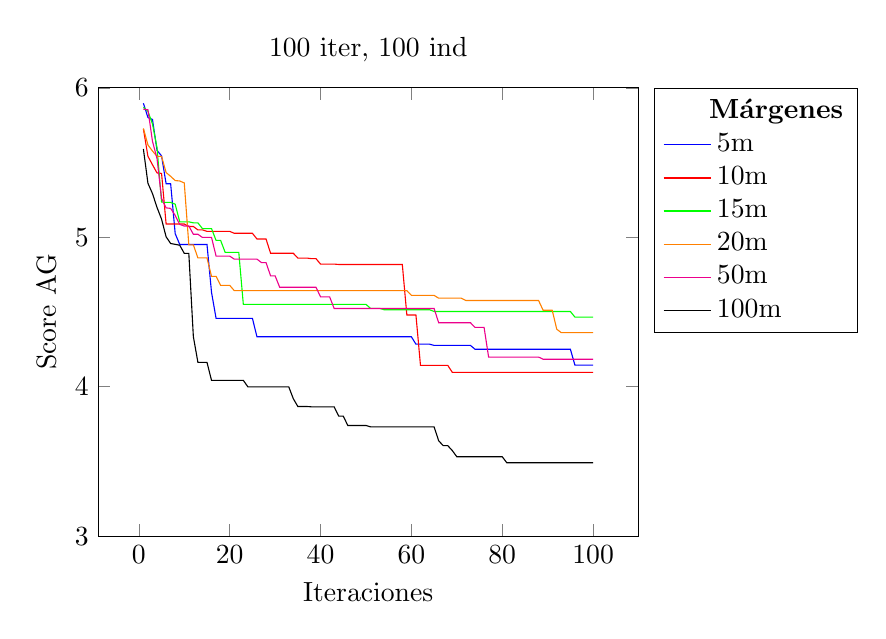
\begin{tikzpicture}[scale=1.0]
      \begin{axis}[
      title={100 iter, 100 ind},
      xlabel={Iteraciones},
      ylabel={Score AG},
      ymin=3,ymax=6,
      legend cell align={left},
      legend pos=outer north east]
      
      \addlegendimage{empty legend}
      
      %\addplot[color=blue] coordinates {(1,5.89722)(2,5.81454)(3,5.83532)(4,5.58186)(5,5.81484)(6,5.55052)(7,5.78918)(8,5.54804)(9,5.64356)(10,5.72724)(11,5.78459)(12,5.82907)(13,5.63125)(14,5.92937)(15,5.71331)(16,5.37907)(17,5.35443)(18,5.77132)(19,5.80576)(20,5.81624)(21,5.82000)(22,5.68595)(23,5.88651)(24,5.62508)(25,5.72692)(26,5.07849)(27,5.54538)(28,5.71954)(29,5.57870)(30,5.62718)(31,5.69319)(32,5.75614)(33,5.72279)(34,5.73874)(35,5.63428)(36,5.51577)(37,5.63244)(38,5.69369)(39,5.67957)(40,5.63122)(41,5.76207)(42,5.62585)(43,5.66328)(44,5.62280)(45,5.61453)(46,5.71047)(47,5.58026)(48,5.49987)(49,5.50661)(50,5.73095)(51,5.65902)(52,5.63884)(53,5.53985)(54,5.51889)(55,5.66092)(56,5.74151)(57,5.65331)(58,5.68137)(59,5.62194)(60,5.63823)(61,5.38061)(62,5.68456)(63,5.68712)(64,5.65594)(65,5.48094)(66,5.68827)(67,5.57239)(68,5.78328)(69,5.85527)(70,5.72950)(71,5.82629)(72,5.84415)(73,5.83899)(74,5.76209)(75,5.80054)(76,5.71885)(77,5.57827)(78,5.70035)(79,5.69906)(80,5.63709)(81,5.70983)(82,5.74680)(83,5.75129)(84,5.70985)(85,5.69730)(86,5.63650)(87,5.79859)(88,5.66832)(89,5.80584)(90,5.77335)(91,5.72521)(92,5.76945)(93,5.80485)(94,5.78661)(95,5.75653)(96,5.28035)(97,5.84041)(98,5.80629)(99,5.92615)(100,5.97531)};
      
      %\addplot[color=red] coordinates {(1,5.72501)(2,5.56216)(3,5.67408)(4,5.56732)(5,5.59471)(6,5.24721)(7,5.79774)(8,5.73755)(9,5.69378)(10,5.80452)(11,5.50950)(12,5.62593)(13,5.47617)(14,5.39066)(15,5.49939)(16,5.53103)(17,5.54317)(18,5.45313)(19,5.49483)(20,5.56563)(21,5.45297)(22,5.45011)(23,5.47514)(24,5.53762)(25,5.58374)(26,5.45450)(27,5.40174)(28,5.55306)(29,5.31201)(30,5.56193)(31,5.43774)(32,5.51165)(33,5.48287)(34,5.73391)(35,5.41981)(36,5.52319)(37,5.55021)(38,5.41039)(39,5.51943)(40,5.41153)(41,5.57425)(42,5.72857)(43,5.56088)(44,5.56362)(45,5.51472)(46,5.70770)(47,5.74962)(48,5.72411)(49,5.64564)(50,5.65608)(51,5.73173)(52,5.47904)(53,5.68952)(54,5.74124)(55,5.67892)(56,5.69919)(57,5.78913)(58,5.61169)(59,5.24727)(60,5.47942)(61,5.63998)(62,4.87307)(63,5.61588)(64,5.58860)(65,5.54351)(66,5.65992)(67,5.49416)(68,5.54376)(69,5.16219)(70,5.46742)(71,5.39017)(72,5.36935)(73,5.50641)(74,5.33081)(75,5.38587)(76,5.42138)(77,5.48940)(78,5.47193)(79,5.48367)(80,5.49855)(81,5.54681)(82,5.54891)(83,5.63250)(84,5.51727)(85,5.52565)(86,5.60200)(87,5.56799)(88,5.53935)(89,5.44074)(90,5.43831)(91,5.42305)(92,5.48174)(93,5.63899)(94,5.53024)(95,5.49729)(96,5.48898)(97,5.52323)(98,5.52460)(99,5.34678)(100,5.48270)};
      
      %\addplot[color=green] coordinates {(1,5.86964)(2,5.90337)(3,5.80148)(4,5.62589)(5,5.29879)(6,5.61972)(7,5.72638)(8,5.54344)(9,5.32753)(10,5.63472)(11,5.68869)(12,5.54517)(13,5.53838)(14,5.56929)(15,5.48377)(16,5.56140)(17,5.24013)(18,5.75168)(19,5.60822)(20,5.64298)(21,5.66704)(22,5.68945)(23,5.47025)(24,5.60230)(25,5.89144)(26,5.89976)(27,6.00766)(28,5.98199)(29,5.84639)(30,5.90715)(31,5.92487)(32,5.94558)(33,5.93975)(34,5.89181)(35,5.83738)(36,5.97997)(37,5.88178)(38,5.85332)(39,5.74613)(40,5.60397)(41,5.63530)(42,5.67598)(43,5.66056)(44,5.79003)(45,5.64366)(46,5.64988)(47,5.64554)(48,5.76579)(49,5.72634)(50,5.41988)(51,5.40842)(52,5.56468)(53,5.51282)(54,5.41861)(55,5.68637)(56,5.68309)(57,5.63366)(58,5.71480)(59,5.64088)(60,5.71088)(61,5.66912)(62,5.62540)(63,5.67352)(64,5.62076)(65,5.51827)(66,5.76301)(67,5.67054)(68,5.38118)(69,5.63952)(70,5.62306)(71,5.54682)(72,5.58980)(73,5.68760)(74,5.63629)(75,5.59675)(76,5.57244)(77,5.58882)(78,5.69082)(79,5.46069)(80,5.79323)(81,5.71893)(82,5.84134)(83,5.75683)(84,5.72583)(85,5.30443)(86,5.54682)(87,5.47502)(88,5.48448)(89,5.60014)(90,5.56790)(91,5.51863)(92,5.59436)(93,5.60591)(94,5.69138)(95,5.57276)(96,5.55922)(97,5.71221)(98,5.67672)(99,5.58090)(100,5.46382)};
      
      %\addplot[color=orange] coordinates {(1,5.72877)(2,5.69577)(3,5.64745)(4,5.58386)(5,5.66184)(6,5.60976)(7,5.75612)(8,5.67747)(9,5.58644)(10,5.61614)(11,5.22682)(12,5.55942)(13,5.54769)(14,5.64817)(15,5.63918)(16,5.53133)(17,5.57513)(18,5.37703)(19,5.57849)(20,5.63805)(21,5.51286)(22,5.56365)(23,5.59656)(24,5.61708)(25,5.67108)(26,5.50521)(27,5.55777)(28,5.74880)(29,5.75823)(30,5.75554)(31,5.64489)(32,5.73459)(33,5.88171)(34,5.58904)(35,5.69511)(36,5.74525)(37,5.71039)(38,5.79738)(39,5.78496)(40,5.70146)(41,5.90202)(42,6.04606)(43,5.88083)(44,6.08728)(45,5.94082)(46,6.08500)(47,5.90711)(48,6.09760)(49,5.41989)(50,5.66483)(51,5.66283)(52,5.59658)(53,5.66559)(54,5.80170)(55,5.57891)(56,5.79291)(57,5.60747)(58,5.73383)(59,5.32966)(60,5.36664)(61,5.60782)(62,5.51685)(63,5.73752)(64,5.79876)(65,5.81634)(66,5.62128)(67,5.87996)(68,5.97407)(69,5.93627)(70,5.78358)(71,5.72135)(72,5.61631)(73,5.47732)(74,5.73574)(75,5.98090)(76,5.99148)(77,5.82701)(78,5.78430)(79,5.71106)(80,5.80476)(81,5.76986)(82,5.60590)(83,5.64637)(84,5.72008)(85,5.72531)(86,5.75660)(87,5.76801)(88,5.69920)(89,5.59503)(90,5.77669)(91,5.48528)(92,5.03424)(93,5.33280)(94,5.64200)(95,5.72585)(96,5.62853)(97,5.61345)(98,5.56623)(99,5.56151)(100,5.55085)};
      
      %\addplot[color=magenta] coordinates {(1,5.85732)(2,6.14023)(3,5.77432)(4,5.87761)(5,5.66408)(6,5.39651)(7,5.78529)(8,5.76898)(9,5.83975)(10,5.57141)(11,6.12072)(12,5.88086)(13,5.64855)(14,5.50218)(15,5.96842)(16,5.89851)(17,5.59432)(18,5.91506)(19,5.85279)(20,5.81429)(21,5.67121)(22,5.63691)(23,5.89967)(24,5.73753)(25,5.82366)(26,5.70195)(27,5.78007)(28,5.85815)(29,5.48677)(30,5.90432)(31,5.47597)(32,6.02114)(33,5.83623)(34,5.85529)(35,5.82517)(36,5.52919)(37,5.62827)(38,5.69055)(39,5.78568)(40,5.43415)(41,5.79103)(42,5.72708)(43,5.59351)(44,5.82947)(45,5.70925)(46,5.52881)(47,5.90791)(48,5.66895)(49,5.81602)(50,5.71407)(51,5.75303)(52,5.89968)(53,5.73375)(54,5.81099)(55,5.64225)(56,5.84861)(57,5.58015)(58,5.64423)(59,5.79940)(60,5.83590)(61,6.02819)(62,5.55867)(63,5.47112)(64,5.65441)(65,5.83863)(66,5.38072)(67,5.67138)(68,5.62874)(69,5.61214)(70,5.72856)(71,5.59628)(72,5.36601)(73,5.54424)(74,5.61169)(75,5.51834)(76,5.54281)(77,5.28068)(78,5.33194)(79,4.84654)(80,5.20773)(81,5.33369)(82,5.29605)(83,5.03217)(84,5.38430)(85,5.37584)(86,5.04720)(87,5.31191)(88,5.42619)(89,5.39961)(90,5.37919)(91,5.38055)(92,5.34949)(93,5.40098)(94,5.61560)(95,5.46876)(96,5.47722)(97,5.25306)(98,4.94529)(99,5.13501)(100,5.27236)};
      
      %\addplot[color=black] coordinates {(1,5.57120)(2,5.57043)(3,5.47904)(4,5.37385)(5,5.50976)(6,5.36388)(7,5.45507)(8,5.51587)(9,5.57892)(10,5.44874)(11,5.61368)(12,4.89732)(13,4.80389)(14,5.61235)(15,5.44252)(16,5.14172)(17,5.43827)(18,5.69915)(19,5.61443)(20,5.72501)(21,5.55194)(22,5.71086)(23,5.57364)(24,5.56846)(25,5.56659)(26,5.59343)(27,5.47216)(28,5.60204)(29,5.65726)(30,5.61998)(31,5.84714)(32,5.66750)(33,5.81376)(34,5.06609)(35,5.65511)(36,5.90210)(37,5.64927)(38,5.96756)(39,5.85213)(40,5.92650)(41,5.91121)(42,5.73251)(43,5.81315)(44,5.47854)(45,5.61384)(46,5.58811)(47,5.60218)(48,5.50630)(49,5.45736)(50,5.46911)(51,5.43671)(52,5.64909)(53,5.58291)(54,5.58500)(55,5.65723)(56,5.60158)(57,5.47279)(58,5.72212)(59,5.70245)(60,5.49413)(61,5.43397)(62,5.44142)(63,5.63240)(64,5.54065)(65,5.26974)(66,5.10360)(67,4.98402)(68,5.21184)(69,5.09390)(70,4.85198)(71,5.44737)(72,5.52683)(73,5.49671)(74,5.57989)(75,5.55883)(76,5.43458)(77,5.40788)(78,5.32809)(79,5.33732)(80,5.43638)(81,5.32184)(82,5.41971)(83,5.43705)(84,5.50601)(85,5.49452)(86,5.40614)(87,5.51031)(88,5.60093)(89,5.13057)(90,5.43902)(91,5.53158)(92,5.64097)(93,5.25789)(94,5.48242)(95,5.54711)(96,5.57862)(97,5.27518)(98,5.38215)(99,5.14171)(100,5.38346)};
      
      \addplot[color=blue] coordinates {(1,5.89724)(2,5.80164)(3,5.78856)(4,5.58186)(5,5.54474)(6,5.35825)(7,5.35825)(8,5.02467)(9,4.95221)(10,4.95221)(11,4.95221)(12,4.95221)(13,4.95221)(14,4.95221)(15,4.95221)(16,4.63134)(17,4.45786)(18,4.45786)(19,4.45786)(20,4.45786)(21,4.45786)(22,4.45786)(23,4.45786)(24,4.45786)(25,4.45786)(26,4.33438)(27,4.33438)(28,4.33438)(29,4.33438)(30,4.33438)(31,4.33438)(32,4.33438)(33,4.33438)(34,4.33438)(35,4.33438)(36,4.33438)(37,4.33438)(38,4.33438)(39,4.33438)(40,4.33438)(41,4.33438)(42,4.33438)(43,4.33438)(44,4.33438)(45,4.33438)(46,4.33438)(47,4.33438)(48,4.33438)(49,4.33438)(50,4.33438)(51,4.33438)(52,4.33438)(53,4.33438)(54,4.33438)(55,4.33438)(56,4.33438)(57,4.33438)(58,4.33438)(59,4.33438)(60,4.33438)(61,4.28483)(62,4.28483)(63,4.28483)(64,4.28483)(65,4.27677)(66,4.27677)(67,4.27677)(68,4.27677)(69,4.27677)(70,4.27677)(71,4.27677)(72,4.27677)(73,4.27677)(74,4.25113)(75,4.25113)(76,4.25113)(77,4.25113)(78,4.25113)(79,4.25113)(80,4.25113)(81,4.25113)(82,4.25113)(83,4.25113)(84,4.25113)(85,4.25113)(86,4.25113)(87,4.25113)(88,4.25113)(89,4.25113)(90,4.25113)(91,4.25113)(92,4.25113)(93,4.25113)(94,4.25113)(95,4.25113)(96,4.14484)(97,4.14484)(98,4.14484)(99,4.14484)(100,4.14484)};
      
      \addplot[color=red] coordinates {(1,5.72501)(2,5.54235)(3,5.48556)(4,5.43081)(5,5.42772)(6,5.08911)(7,5.08911)(8,5.08911)(9,5.08911)(10,5.08911)(11,5.07235)(12,5.07235)(13,5.04970)(14,5.04970)(15,5.03994)(16,5.03994)(17,5.03994)(18,5.03994)(19,5.03994)(20,5.03994)(21,5.02694)(22,5.02694)(23,5.02694)(24,5.02694)(25,5.02694)(26,4.98874)(27,4.98874)(28,4.98874)(29,4.89322)(30,4.89322)(31,4.89322)(32,4.89322)(33,4.89322)(34,4.89322)(35,4.86117)(36,4.86117)(37,4.86117)(38,4.85700)(39,4.85700)(40,4.82070)(41,4.82070)(42,4.82070)(43,4.82070)(44,4.81830)(45,4.81830)(46,4.81830)(47,4.81830)(48,4.81830)(49,4.81830)(50,4.81830)(51,4.81830)(52,4.81830)(53,4.81830)(54,4.81830)(55,4.81830)(56,4.81830)(57,4.81830)(58,4.81830)(59,4.47996)(60,4.47996)(61,4.47996)(62,4.14344)(63,4.14344)(64,4.14344)(65,4.14344)(66,4.14344)(67,4.14344)(68,4.14344)(69,4.09664)(70,4.09664)(71,4.09664)(72,4.09664)(73,4.09664)(74,4.09664)(75,4.09664)(76,4.09664)(77,4.09664)(78,4.09664)(79,4.09664)(80,4.09664)(81,4.09664)(82,4.09664)(83,4.09664)(84,4.09664)(85,4.09664)(86,4.09664)(87,4.09664)(88,4.09664)(89,4.09664)(90,4.09664)(91,4.09664)(92,4.09664)(93,4.09664)(94,4.09664)(95,4.09664)(96,4.09664)(97,4.09664)(98,4.09664)(99,4.09664)(100,4.09664)};
      
      \addplot[color=green] coordinates {(1,5.86964)(2,5.84361)(3,5.75885)(4,5.60006)(5,5.23578)(6,5.23334)(7,5.23334)(8,5.22179)(9,5.10363)(10,5.10363)(11,5.10363)(12,5.09685)(13,5.09685)(14,5.05797)(15,5.05797)(16,5.05797)(17,4.97943)(18,4.97943)(19,4.89943)(20,4.89943)(21,4.89943)(22,4.89943)(23,4.55152)(24,4.55152)(25,4.55152)(26,4.55152)(27,4.55152)(28,4.55152)(29,4.55152)(30,4.55152)(31,4.55152)(32,4.55152)(33,4.55152)(34,4.55152)(35,4.55152)(36,4.55152)(37,4.55152)(38,4.55152)(39,4.55152)(40,4.55152)(41,4.55152)(42,4.55152)(43,4.55152)(44,4.55152)(45,4.55152)(46,4.55152)(47,4.55152)(48,4.55152)(49,4.55152)(50,4.55152)(51,4.52454)(52,4.52454)(53,4.52454)(54,4.51540)(55,4.51540)(56,4.51540)(57,4.51540)(58,4.51540)(59,4.51540)(60,4.51540)(61,4.51540)(62,4.51540)(63,4.51540)(64,4.51540)(65,4.50364)(66,4.50364)(67,4.50364)(68,4.50364)(69,4.50364)(70,4.50364)(71,4.50364)(72,4.50364)(73,4.50364)(74,4.50364)(75,4.50364)(76,4.50364)(77,4.50364)(78,4.50364)(79,4.50364)(80,4.50364)(81,4.50364)(82,4.50364)(83,4.50364)(84,4.50364)(85,4.50364)(86,4.50364)(87,4.50364)(88,4.50364)(89,4.50364)(90,4.50364)(91,4.50364)(92,4.50364)(93,4.50364)(94,4.50364)(95,4.50364)(96,4.46589)(97,4.46589)(98,4.46589)(99,4.46589)(100,4.46589)};
      
      \addplot[color=orange] coordinates {(1,5.72877)(2,5.61829)(3,5.57733)(4,5.54186)(5,5.54186)(6,5.43350)(7,5.40810)(8,5.37981)(9,5.37698)(10,5.36367)(11,4.94946)(12,4.94946)(13,4.86193)(14,4.86193)(15,4.86193)(16,4.73897)(17,4.73897)(18,4.67881)(19,4.67881)(20,4.67881)(21,4.64325)(22,4.64325)(23,4.64325)(24,4.64325)(25,4.64325)(26,4.64325)(27,4.64325)(28,4.64325)(29,4.64325)(30,4.64325)(31,4.64325)(32,4.64325)(33,4.64325)(34,4.64325)(35,4.64325)(36,4.64325)(37,4.64325)(38,4.64325)(39,4.64325)(40,4.64325)(41,4.64325)(42,4.64325)(43,4.64325)(44,4.64325)(45,4.64325)(46,4.64325)(47,4.64325)(48,4.64325)(49,4.64325)(50,4.64325)(51,4.64325)(52,4.64325)(53,4.64325)(54,4.64325)(55,4.64325)(56,4.64325)(57,4.64325)(58,4.64325)(59,4.64325)(60,4.61159)(61,4.61159)(62,4.61159)(63,4.61159)(64,4.61159)(65,4.61159)(66,4.59260)(67,4.59260)(68,4.59260)(69,4.59260)(70,4.59260)(71,4.59260)(72,4.57703)(73,4.57703)(74,4.57703)(75,4.57703)(76,4.57703)(77,4.57703)(78,4.57703)(79,4.57703)(80,4.57703)(81,4.57703)(82,4.57703)(83,4.57703)(84,4.57703)(85,4.57703)(86,4.57703)(87,4.57703)(88,4.57703)(89,4.51189)(90,4.51189)(91,4.51189)(92,4.38520)(93,4.36183)(94,4.36183)(95,4.36183)(96,4.36183)(97,4.36183)(98,4.36183)(99,4.36183)(100,4.36183)};
      
      \addplot[color=magenta] coordinates {(1,5.85732)(2,5.85369)(3,5.64253)(4,5.52707)(5,5.25948)(6,5.19690)(7,5.19368)(8,5.14651)(9,5.08593)(10,5.07560)(11,5.07560)(12,5.02050)(13,5.02050)(14,4.99912)(15,4.99912)(16,4.99912)(17,4.87433)(18,4.87433)(19,4.87433)(20,4.87433)(21,4.85421)(22,4.85421)(23,4.85421)(24,4.85421)(25,4.85421)(26,4.85421)(27,4.83060)(28,4.83060)(29,4.74225)(30,4.74225)(31,4.66578)(32,4.66578)(33,4.66578)(34,4.66578)(35,4.66578)(36,4.66578)(37,4.66578)(38,4.66578)(39,4.66578)(40,4.60169)(41,4.60169)(42,4.60169)(43,4.52339)(44,4.52339)(45,4.52339)(46,4.52339)(47,4.52339)(48,4.52339)(49,4.52339)(50,4.52339)(51,4.52339)(52,4.52339)(53,4.52339)(54,4.52339)(55,4.52339)(56,4.52339)(57,4.52339)(58,4.52339)(59,4.52339)(60,4.52339)(61,4.52339)(62,4.52339)(63,4.52339)(64,4.52339)(65,4.52339)(66,4.42861)(67,4.42861)(68,4.42861)(69,4.42861)(70,4.42861)(71,4.42861)(72,4.42861)(73,4.42861)(74,4.39689)(75,4.39689)(76,4.39689)(77,4.19858)(78,4.19858)(79,4.19858)(80,4.19858)(81,4.19858)(82,4.19858)(83,4.19858)(84,4.19858)(85,4.19858)(86,4.19858)(87,4.19858)(88,4.19858)(89,4.18431)(90,4.18431)(91,4.18431)(92,4.18431)(93,4.18431)(94,4.18431)(95,4.18431)(96,4.18431)(97,4.18431)(98,4.18431)(99,4.18431)(100,4.18431)};
      
      \addplot[color=black] coordinates {(1,5.59087)(2,5.36161)(3,5.29254)(4,5.19986)(5,5.12146)(6,5.00336)(7,4.95849)(8,4.95300)(9,4.94697)(10,4.89287)(11,4.89287)(12,4.33498)(13,4.16360)(14,4.16360)(15,4.16261)(16,4.04276)(17,4.04276)(18,4.04276)(19,4.04276)(20,4.04276)(21,4.04276)(22,4.04276)(23,4.04276)(24,3.99941)(25,3.99941)(26,3.99941)(27,3.99941)(28,3.99941)(29,3.99941)(30,3.99941)(31,3.99941)(32,3.99941)(33,3.99941)(34,3.92046)(35,3.86786)(36,3.86786)(37,3.86786)(38,3.86560)(39,3.86560)(40,3.86560)(41,3.86560)(42,3.86560)(43,3.86560)(44,3.80366)(45,3.80366)(46,3.74089)(47,3.74089)(48,3.74089)(49,3.74089)(50,3.74089)(51,3.73182)(52,3.73182)(53,3.73182)(54,3.73182)(55,3.73182)(56,3.73182)(57,3.73182)(58,3.73182)(59,3.73182)(60,3.73182)(61,3.73182)(62,3.73182)(63,3.73182)(64,3.73182)(65,3.73182)(66,3.63871)(67,3.60603)(68,3.60603)(69,3.57322)(70,3.53152)(71,3.53152)(72,3.53152)(73,3.53152)(74,3.53152)(75,3.53152)(76,3.53152)(77,3.53152)(78,3.53152)(79,3.53152)(80,3.53152)(81,3.49166)(82,3.49166)(83,3.49166)(84,3.49166)(85,3.49166)(86,3.49166)(87,3.49166)(88,3.49166)(89,3.49166)(90,3.49166)(91,3.49166)(92,3.49166)(93,3.49166)(94,3.49166)(95,3.49166)(96,3.49166)(97,3.49166)(98,3.49166)(99,3.49166)(100,3.49166)};
      
      \addlegendentry{\hspace{-.1cm}\textbf{Márgenes}}
        \addlegendentry{5m}
        \addlegendentry{10m}
        \addlegendentry{15m}
        \addlegendentry{20m}
        \addlegendentry{50m}
        \addlegendentry{100m}
        
      \end{axis}
    \end{tikzpicture}
    \caption{Ejecuciones con diferentes márgenes (mod. mixto)}
    \label{fig:adv_multi_margin_mixed}
\end{figure}

Como se puede observar en la figura \ref{fig:adv_multi_margin_mixed}, donde cada una de las series de datos se corresponden a la media de las mejores puntuaciones obtenidas hasta dicha iteración, el efecto resultante de elegir un margen distinto para realizar una ejecución del sistema es similar al de la prueba anterior. Como pasaba con el métricas basadas en la mejora del tiempo de ruta, para los márgenes con valores más pequeños, durante toda la ejecución, el mejor valor de dicho instante se mantiene prácticamente en el mismo rango, incluyendo también aquí el margen de 50 metros.

Comparando estas puntuaciones, es claramente visible, como, en este caso, el utilizar el margen de 100 puntos otorga una mejora sustancial en los resultados finales del modelo, estando estos muy por debajo (a menor valor de \textit{fitness}, mejor se considera el resultado) del resto de márgenes utilizados.

Para este grupo de resultados mostrados, se ha utilizado un factor $r$ de ponderación de 0.5, es decir, un peso por igual al consumo y el tiempo empleado. Es por ello, que, por ejemplo, al obtener el consumo medio y tiempo empleado por márgenes, la diferencia entre las opciones no es tan destacada. En el caso del mejor margen, de 100 metros, la media de consumo estimada para esa ruta es de 17,2 kWh en un tiempo de 17 minutos, mientras que, en el margen de 15 metros, de media el consumo estimado es ligeramente menor, de 16,8 kWh, pero en un mayor tiempo, 18 minutos.

\newpage
\subsection{Pruebas adicionales}
Además de las pruebas ya descritas anteriormente, y que se correspondían a una métrica específica por sección, en este último punto de pruebas se encuentran aquellas en las que o bien se han probado configuraciones del sistema diferentes a las mencionadas, o se comparan los resultados de una configuración específica sobre una o varios métricas a la vez.\newline

\textbf{Incremento del número de individuos}\newline
Pese a lo que ya se había demostrado anteriormente entre las comparaciones de 30 y 100 individuos, aprovechando los buenos resultados obtenidos con las métricas de optimización mixtas y el margen de 100 metros de distancia entre puntos, se ha utilizado dicha configuración para ver los posibles efectos de ampliar la población una tercera vez hasta un grupo de 200 individuos o el paso intermedio entre 30 y 100.

% FIGURE 34
\begin{figure}[!htb]
    \centering
    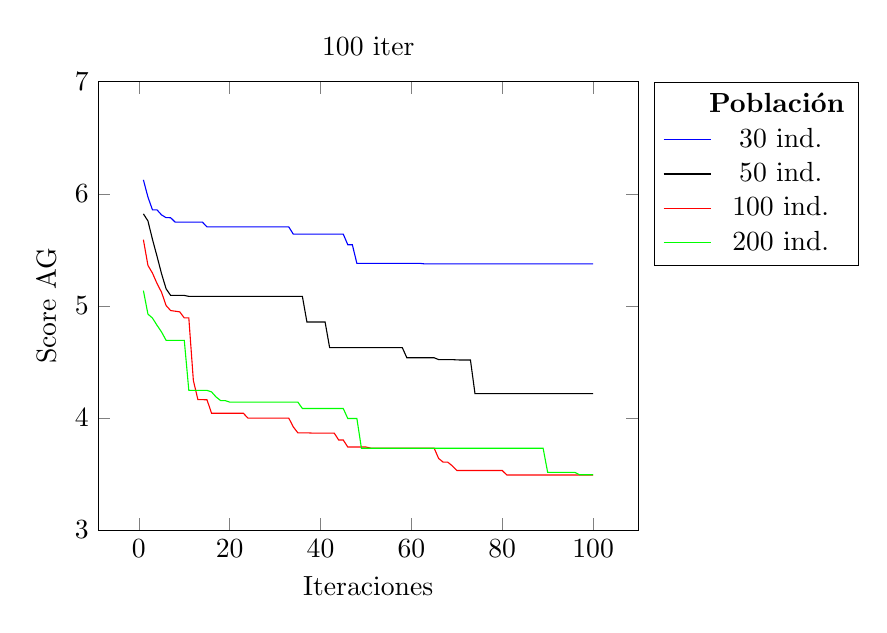
\begin{tikzpicture}[scale=1.0]
      \begin{axis}[
      title={100 iter},
      xlabel={Iteraciones},
      ylabel={Score AG},
      ymin=3,ymax=7,
      legend pos=outer north east]
      
      \addlegendimage{empty legend}
      
      \addplot[color=blue] coordinates {(1,6.12463)(2,5.97129)(3,5.85676)(4,5.85676)(5,5.81200)(6,5.78728)(7,5.78707)(8,5.74736)(9,5.74736)(10,5.74736)(11,5.74736)(12,5.74736)(13,5.74736)(14,5.74736)(15,5.70500)(16,5.70500)(17,5.70500)(18,5.70500)(19,5.70500)(20,5.70500)(21,5.70500)(22,5.70500)(23,5.70500)(24,5.70500)(25,5.70500)(26,5.70500)(27,5.70500)(28,5.70500)(29,5.70500)(30,5.70500)(31,5.70500)(32,5.70500)(33,5.70500)(34,5.64034)(35,5.64034)(36,5.64034)(37,5.64034)(38,5.64034)(39,5.64034)(40,5.64034)(41,5.64034)(42,5.64034)(43,5.64034)(44,5.64034)(45,5.64034)(46,5.54569)(47,5.54569)(48,5.37915)(49,5.37915)(50,5.37915)(51,5.37915)(52,5.37915)(53,5.37915)(54,5.37915)(55,5.37915)(56,5.37915)(57,5.37915)(58,5.37915)(59,5.37915)(60,5.37915)(61,5.37915)(62,5.37915)(63,5.37465)(64,5.37465)(65,5.37465)(66,5.37465)(67,5.37465)(68,5.37465)(69,5.37465)(70,5.37465)(71,5.37465)(72,5.37465)(73,5.37465)(74,5.37465)(75,5.37465)(76,5.37465)(77,5.37465)(78,5.37465)(79,5.37465)(80,5.37465)(81,5.37465)(82,5.37465)(83,5.37465)(84,5.37465)(85,5.37465)(86,5.37465)(87,5.37465)(88,5.37465)(89,5.37465)(90,5.37465)(91,5.37465)(92,5.37465)(93,5.37465)(94,5.37465)(95,5.37465)(96,5.37465)(97,5.37465)(98,5.37465)(99,5.37465)(100,5.37465)};
      
      \addplot[color=black] coordinates {(1,5.82166)(2,5.75826)(3,5.59328)(4,5.44289)(5,5.28669)(6,5.15250)(7,5.09356)(8,5.09356)(9,5.09356)(10,5.09356)(11,5.08530)(12,5.08530)(13,5.08530)(14,5.08530)(15,5.08530)(16,5.08530)(17,5.08530)(18,5.08530)(19,5.08530)(20,5.08530)(21,5.08530)(22,5.08530)(23,5.08530)(24,5.08530)(25,5.08530)(26,5.08530)(27,5.08530)(28,5.08530)(29,5.08530)(30,5.08530)(31,5.08530)(32,5.08530)(33,5.08530)(34,5.08530)(35,5.08530)(36,5.08530)(37,4.85658)(38,4.85658)(39,4.85658)(40,4.85658)(41,4.85658)(42,4.62770)(43,4.62770)(44,4.62770)(45,4.62766)(46,4.62765)(47,4.62764)(48,4.62764)(49,4.62764)(50,4.62764)(51,4.62764)(52,4.62764)(53,4.62764)(54,4.62764)(55,4.62764)(56,4.62764)(57,4.62764)(58,4.62764)(59,4.53743)(60,4.53743)(61,4.53743)(62,4.53743)(63,4.53743)(64,4.53743)(65,4.53743)(66,4.52132)(67,4.52132)(68,4.52132)(69,4.52132)(70,4.51836)(71,4.51742)(72,4.51742)(73,4.51742)(74,4.21705)(75,4.21705)(76,4.21705)(77,4.21705)(78,4.21705)(79,4.21705)(80,4.21705)(81,4.21705)(82,4.21705)(83,4.21705)(84,4.21705)(85,4.21705)(86,4.21705)(87,4.21705)(88,4.21705)(89,4.21705)(90,4.21705)(91,4.21705)(92,4.21705)(93,4.21705)(94,4.21705)(95,4.21705)(96,4.21705)(97,4.21705)(98,4.21705)(99,4.21705)(100,4.21705)};
      
      \addplot[color=red] coordinates {(1,5.59087)(2,5.36161)(3,5.29254)(4,5.19986)(5,5.12146)(6,5.00336)(7,4.95849)(8,4.95300)(9,4.94697)(10,4.89287)(11,4.89287)(12,4.33498)(13,4.16360)(14,4.16360)(15,4.16261)(16,4.04276)(17,4.04276)(18,4.04276)(19,4.04276)(20,4.04276)(21,4.04276)(22,4.04276)(23,4.04276)(24,3.99941)(25,3.99941)(26,3.99941)(27,3.99941)(28,3.99941)(29,3.99941)(30,3.99941)(31,3.99941)(32,3.99941)(33,3.99941)(34,3.92046)(35,3.86786)(36,3.86786)(37,3.86786)(38,3.86560)(39,3.86560)(40,3.86560)(41,3.86560)(42,3.86560)(43,3.86560)(44,3.80366)(45,3.80366)(46,3.74089)(47,3.74089)(48,3.74089)(49,3.74089)(50,3.74089)(51,3.73182)(52,3.73182)(53,3.73182)(54,3.73182)(55,3.73182)(56,3.73182)(57,3.73182)(58,3.73182)(59,3.73182)(60,3.73182)(61,3.73182)(62,3.73182)(63,3.73182)(64,3.73182)(65,3.73182)(66,3.63871)(67,3.60603)(68,3.60603)(69,3.57322)(70,3.53152)(71,3.53152)(72,3.53152)(73,3.53152)(74,3.53152)(75,3.53152)(76,3.53152)(77,3.53152)(78,3.53152)(79,3.53152)(80,3.53152)(81,3.49166)(82,3.49166)(83,3.49166)(84,3.49166)(85,3.49166)(86,3.49166)(87,3.49166)(88,3.49166)(89,3.49166)(90,3.49166)(91,3.49166)(92,3.49166)(93,3.49166)(94,3.49166)(95,3.49166)(96,3.49166)(97,3.49166)(98,3.49166)(99,3.49166)(100,3.49166)};
      
      \addplot[color=green] coordinates {(1,5.13686)(2,4.92711)(3,4.89145)(4,4.82707)(5,4.76750)(6,4.69257)(7,4.69257)(8,4.69257)(9,4.69257)(10,4.69257)(11,4.24642)(12,4.24642)(13,4.24642)(14,4.24642)(15,4.24642)(16,4.23292)(17,4.18773)(18,4.15557)(19,4.15557)(20,4.14185)(21,4.14185)(22,4.14185)(23,4.14185)(24,4.14185)(25,4.14185)(26,4.14185)(27,4.14185)(28,4.14185)(29,4.14185)(30,4.14185)(31,4.14185)(32,4.14185)(33,4.14185)(34,4.14185)(35,4.14185)(36,4.08464)(37,4.08464)(38,4.08464)(39,4.08464)(40,4.08464)(41,4.08464)(42,4.08464)(43,4.08464)(44,4.08464)(45,4.08464)(46,3.99542)(47,3.99542)(48,3.99542)(49,3.73011)(50,3.73011)(51,3.73011)(52,3.73011)(53,3.73011)(54,3.73011)(55,3.73011)(56,3.73011)(57,3.73011)(58,3.73011)(59,3.73011)(60,3.73011)(61,3.73011)(62,3.73011)(63,3.73011)(64,3.73011)(65,3.73011)(66,3.73011)(67,3.73011)(68,3.73011)(69,3.73011)(70,3.73011)(71,3.73011)(72,3.73011)(73,3.73011)(74,3.73011)(75,3.73011)(76,3.73011)(77,3.73011)(78,3.73011)(79,3.73011)(80,3.73011)(81,3.73011)(82,3.73011)(83,3.73011)(84,3.73011)(85,3.73011)(86,3.73011)(87,3.73011)(88,3.73011)(89,3.73011)(90,3.51461)(91,3.51461)(92,3.51461)(93,3.51461)(94,3.51461)(95,3.51461)(96,3.51461)(97,3.49372)(98,3.49372)(99,3.49372)(100,3.49372)};
      
        \addlegendentry{\hspace{-.1cm}\textbf{Población}}
        \addlegendentry{30 ind.}
        \addlegendentry{50 ind.}
        \addlegendentry{100 ind.}
        \addlegendentry{200 ind.}
      
      \end{axis}
    \end{tikzpicture}
    \caption{Ejecuciones con diferentes poblaciones (mod. mixto)}
    \label{fig:adv_multi_pop_mixed}
\end{figure}

Como se puede ver en la figura \ref{fig:adv_multi_pop_mixed}, mientras que sí que hay una influencia en el resultado conforme se incrementa el número de individuos de 30 hasta 100, el incremento de 100 a 200 no llega a aportar ninguna mejora a dichos resultados. Prácticamente durante todas las iteraciones, las poblaciones de 100 y 200 individuos se mantienen en el mismo rango de resultados. Es por ello, que, ante esta igualdad, sería preferible, en caso de utilizar estas métricas mixtas, una población de 100 individuos, ya que supone una reducción considerable en el tiempo de cómputo para obtener estos resultados.\newline

\textbf{Diferentes factores para las métricas mixtas}\newline
Otro de los puntos probados se trata de la comprobación del efecto que se produce en los resultados al modificar el factor $r$ utilizado en la ponderación de los valores de \textit{fitness} obtenidos durante la ejecución del modelo avanzado junto al uso de métricas mixtas. Mientras que las pruebas realizadas en la sección \ref{section:mix_model_tests} utilizaban un factor de $r$ de 0.5 (igual consideración a consumo y tiempo), para esta prueba se ha modificado dicho valor a 0.25 y 0.75, siendo 0.25 donde se prima más el tiempo consumido en realizar la ruta y 0.75 donde se prima más el consumo eléctrico realizado.

El resultado de estas pruebas puede observarse en la figura \ref{fig:adv_multi_r_mixed}. En esta, se pueden observar tres tendencias diferentes. Por un lado, destaca el hecho de cómo, al priorizar los consumos ($r=0.75$), la capacidad de mejora del sistema es menor, obteniendo unos resultados no tan buenos respecto a las otras opciones según van avanzando las iteraciones.

% FIGURE 35
\begin{figure}[!htb]
    \centering
    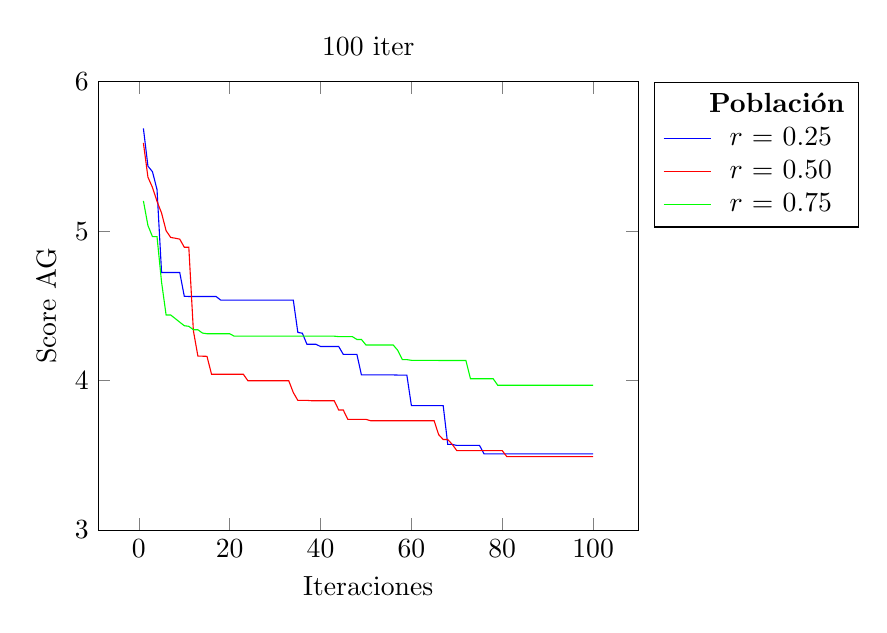
\begin{tikzpicture}[scale=1.0]
      \begin{axis}[
      title={100 iter},
      xlabel={Iteraciones},
      ylabel={Score AG},
      ymin=3,ymax=6,
      legend pos=outer north east]
      
      \addlegendimage{empty legend}
      
      \addplot[color=blue] coordinates {(1,5.68842)(2,5.43529)(3,5.39784)(4,5.27862)(5,4.72388)(6,4.72388)(7,4.72388)(8,4.72388)(9,4.72388)(10,4.56472)(11,4.56315)(12,4.56315)(13,4.56315)(14,4.56315)(15,4.56315)(16,4.56315)(17,4.56315)(18,4.53911)(19,4.53911)(20,4.53911)(21,4.53911)(22,4.53911)(23,4.53911)(24,4.53911)(25,4.53911)(26,4.53911)(27,4.53911)(28,4.53911)(29,4.53911)(30,4.53911)(31,4.53911)(32,4.53911)(33,4.53911)(34,4.53911)(35,4.32288)(36,4.31722)(37,4.24327)(38,4.24327)(39,4.24327)(40,4.22835)(41,4.22835)(42,4.22835)(43,4.22835)(44,4.22835)(45,4.17573)(46,4.17573)(47,4.17573)(48,4.17573)(49,4.03839)(50,4.03839)(51,4.03839)(52,4.03839)(53,4.03839)(54,4.03839)(55,4.03835)(56,4.03829)(57,4.03728)(58,4.03717)(59,4.03717)(60,3.83310)(61,3.83310)(62,3.83310)(63,3.83310)(64,3.83310)(65,3.83310)(66,3.83310)(67,3.83310)(68,3.57397)(69,3.57321)(70,3.56644)(71,3.56644)(72,3.56644)(73,3.56644)(74,3.56644)(75,3.56644)(76,3.50954)(77,3.50954)(78,3.50954)(79,3.50954)(80,3.50954)(81,3.50954)(82,3.50954)(83,3.50954)(84,3.50954)(85,3.50954)(86,3.50954)(87,3.50954)(88,3.50954)(89,3.50954)(90,3.50954)(91,3.50954)(92,3.50954)(93,3.50954)(94,3.50954)(95,3.50954)(96,3.50954)(97,3.50954)(98,3.50954)(99,3.50954)(100,3.50954)};
      
      \addplot[color=red] coordinates {(1,5.59087)(2,5.36161)(3,5.29254)(4,5.19986)(5,5.12146)(6,5.00336)(7,4.95849)(8,4.95300)(9,4.94697)(10,4.89287)(11,4.89287)(12,4.33498)(13,4.16360)(14,4.16360)(15,4.16261)(16,4.04276)(17,4.04276)(18,4.04276)(19,4.04276)(20,4.04276)(21,4.04276)(22,4.04276)(23,4.04276)(24,3.99941)(25,3.99941)(26,3.99941)(27,3.99941)(28,3.99941)(29,3.99941)(30,3.99941)(31,3.99941)(32,3.99941)(33,3.99941)(34,3.92046)(35,3.86786)(36,3.86786)(37,3.86786)(38,3.86560)(39,3.86560)(40,3.86560)(41,3.86560)(42,3.86560)(43,3.86560)(44,3.80366)(45,3.80366)(46,3.74089)(47,3.74089)(48,3.74089)(49,3.74089)(50,3.74089)(51,3.73182)(52,3.73182)(53,3.73182)(54,3.73182)(55,3.73182)(56,3.73182)(57,3.73182)(58,3.73182)(59,3.73182)(60,3.73182)(61,3.73182)(62,3.73182)(63,3.73182)(64,3.73182)(65,3.73182)(66,3.63871)(67,3.60603)(68,3.60603)(69,3.57322)(70,3.53152)(71,3.53152)(72,3.53152)(73,3.53152)(74,3.53152)(75,3.53152)(76,3.53152)(77,3.53152)(78,3.53152)(79,3.53152)(80,3.53152)(81,3.49166)(82,3.49166)(83,3.49166)(84,3.49166)(85,3.49166)(86,3.49166)(87,3.49166)(88,3.49166)(89,3.49166)(90,3.49166)(91,3.49166)(92,3.49166)(93,3.49166)(94,3.49166)(95,3.49166)(96,3.49166)(97,3.49166)(98,3.49166)(99,3.49166)(100,3.49166)};
      
      \addplot[color=green] coordinates {(1,5.20295)(2,5.03810)(3,4.96335)(4,4.96335)(5,4.65940)(6,4.43951)(7,4.43951)(8,4.41566)(9,4.39125)(10,4.36757)(11,4.36336)(12,4.34047)(13,4.34047)(14,4.31830)(15,4.31385)(16,4.31385)(17,4.31385)(18,4.31385)(19,4.31385)(20,4.31385)(21,4.29751)(22,4.29751)(23,4.29751)(24,4.29751)(25,4.29751)(26,4.29751)(27,4.29751)(28,4.29751)(29,4.29751)(30,4.29751)(31,4.29751)(32,4.29751)(33,4.29751)(34,4.29751)(35,4.29751)(36,4.29751)(37,4.29751)(38,4.29751)(39,4.29751)(40,4.29751)(41,4.29751)(42,4.29751)(43,4.29751)(44,4.29457)(45,4.29457)(46,4.29457)(47,4.29457)(48,4.27559)(49,4.27559)(50,4.23852)(51,4.23852)(52,4.23852)(53,4.23852)(54,4.23852)(55,4.23852)(56,4.23852)(57,4.20252)(58,4.14059)(59,4.14059)(60,4.13591)(61,4.13591)(62,4.13591)(63,4.13591)(64,4.13591)(65,4.13591)(66,4.13502)(67,4.13502)(68,4.13502)(69,4.13502)(70,4.13502)(71,4.13502)(72,4.13502)(73,4.01276)(74,4.01276)(75,4.01276)(76,4.01276)(77,4.01276)(78,4.01276)(79,3.96947)(80,3.96947)(81,3.96947)(82,3.96947)(83,3.96947)(84,3.96947)(85,3.96947)(86,3.96947)(87,3.96947)(88,3.96947)(89,3.96947)(90,3.96947)(91,3.96947)(92,3.96947)(93,3.96947)(94,3.96947)(95,3.96947)(96,3.96947)(97,3.96947)(98,3.96947)(99,3.96947)(100,3.96947)};
      
        \addlegendentry{\hspace{-.1cm}\textbf{Población}}
        \addlegendentry{$r$ = 0.25}
        \addlegendentry{$r$ = 0.50}
        \addlegendentry{$r$ = 0.75}
      
      \end{axis}
    \end{tikzpicture}
    \caption{Ejecuciones con diferentes factores (métrica mixta)}
    \label{fig:adv_multi_r_mixed}
\end{figure}

Por otro lado, se observa como al priorizar el tiempo ($r=0.75$) ocurre un poco el efecto contrario; mientras que en las primeras iteraciones los mejores resultados obtenidos son peores que las otras opciones, con el avance en las iteraciones, estos van mejorando hasta situarse a la par que en la configuración con el mismo peso para ambos factores ($r=0.5$), siendo las puntuaciones de \textit{fitness} obtenidas prácticamente idénticas.

Con estos resultados relativos al valor de \textit{fitness} del algoritmo genético, los valores asociados al consumo y al tiempo empleado en cada opción se corresponden a los mostrados en la tabla \ref{tab:adv_simulation_r_mix_res}. En esta se puede observar, efectivamente, como cambiando el valor de $r$, los consumos y tiempos obtenidos se adaptan a los que se pretenden buscar.\newline

\begin{table}[!htb]
    \centering
    \begin{tabular}{m{0.25\textwidth}*2c}
    \toprule
    \multirow{3}*{\textbf{Métrica}} & \multicolumn{2}{c}{\textbf{Métricas mixtas}} \\
     & \textbf{Consumo (kWh)} & \textbf{Tiempo (min)} \\
    \midrule
    \textbf{Mejor Tiempo} & 20,0 & 14,4 \\
    \textbf{Media} & 17,2 & 17,1 \\
    \textbf{Mejor Consumo} & 15,2 & 21 \\
    \bottomrule
    \end{tabular}
    \caption{Valores de consumo y tiempo según factor $r$}
    \label{tab:adv_simulation_r_mix_res}
\end{table}

\textbf{Comparación entre diferentes vehículos}\newline
Esta última prueba, consiste en poder observar que efecto tiene sobre los resultados elegir un vehículo diferente para realizar el proceso de optimización. Para ello, la métrica utilizada en esta prueba se trata de la utilizada por el modelo avanzado inicialmente, es decir, basada en la mejora de los consumo eléctricos realizados por el vehículo durante la ruta, de forma que se puede apreciar más claramente el efecto resultante al cambiar entre los diferentes vehículos.

% FIGURE 36
\begin{figure}[!htb]
    \centering
    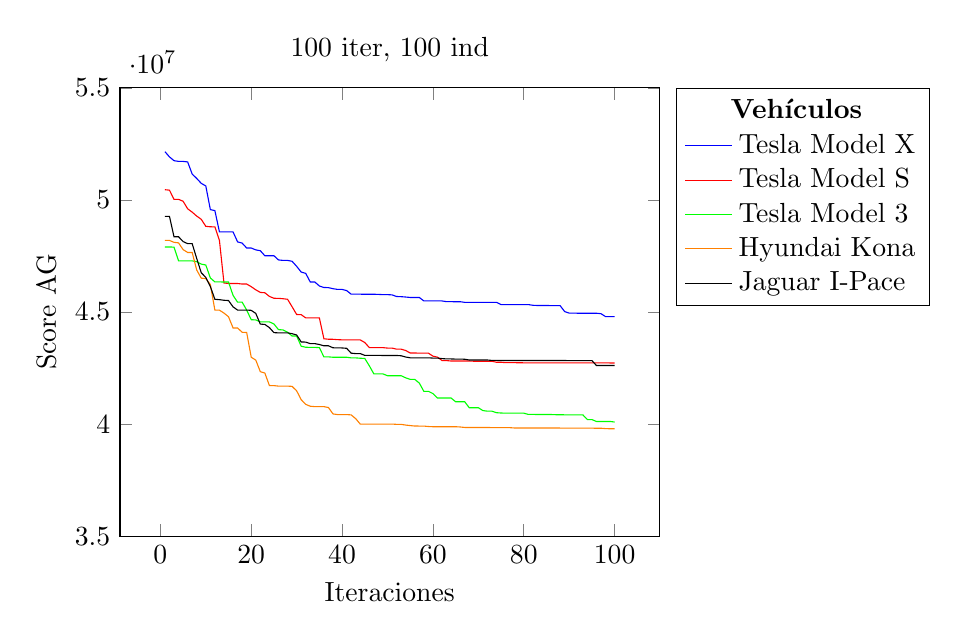
\begin{tikzpicture}[scale=1.0]
      \begin{axis}[
      title={100 iter, 100 ind},
      xlabel={Iteraciones},
      ylabel={Score AG},
      ymin=35000000,ymax=55000000,
      legend cell align={left},
      legend pos=outer north east]
      
      \addlegendimage{empty legend}
      
      %\addplot[color=blue] coordinates {(1,52154717.10700)(2,51936265.40452)(3,51948926.28814)(4,51991474.09393)(5,51989998.73701)(6,51912935.83564)(7,51352161.31480)(8,51152703.68221)(9,51057604.38941)(10,50903965.05935)(11,49899979.30886)(12,49854362.25188)(13,48577897.26408)(14,48846709.92406)(15,48856824.90557)(16,48865668.81183)(17,48395682.01270)(18,48341436.24676)(19,48120139.07223)(20,48159175.69341)(21,47809946.26889)(22,47772067.73684)(23,47570399.19078)(24,47571967.60990)(25,47572166.82242)(26,47349674.38000)(27,47328474.05380)(28,47328474.05380)(29,47289176.76523)(30,47064376.34729)(31,46808260.64406)(32,46724917.50756)(33,46344558.43703)(34,46722809.07358)(35,46544219.34140)(36,46473448.94135)(37,46466388.91886)(38,46418003.88488)(39,46346365.23117)(40,46346365.23117)(41,46295145.72066)(42,46132269.44370)(43,46117085.18859)(44,46116366.98732)(45,46099947.00619)(46,46099947.00619)(47,46099947.00619)(48,46093544.17168)(49,46060203.49514)(50,46069054.62033)(51,46058532.16708)(52,45996744.43775)(53,45769535.14566)(54,45976925.76478)(55,45922549.47438)(56,45925350.19027)(57,45916649.00762)(58,45758178.17168)(59,45747956.00880)(60,45727685.10813)(61,45558650.96081)(62,45572333.59276)(63,45536737.68502)(64,45503974.55765)(65,45498142.50421)(66,45511473.74724)(67,45482702.84165)(68,45475469.94547)(69,45475469.94547)(70,45475469.94547)(71,45475553.36877)(72,45475553.36877)(73,45491341.19368)(74,45491341.19368)(75,45392468.89658)(76,45392468.89658)(77,45392468.89658)(78,45388534.02253)(79,45366803.07981)(80,45367670.45187)(81,45358876.20888)(82,45322475.65357)(83,45312429.49548)(84,45312554.40285)(85,45309103.66125)(86,45296693.30135)(87,45297221.64595)(88,45298162.81447)(89,45033238.69646)(90,44962471.44297)(91,44962476.35661)(92,44961929.72950)(93,44963924.69888)(94,44963924.73451)(95,44963924.73451)(96,44963925.24107)(97,44941782.35683)(98,44807689.82240)(99,44807724.34900)(100,44807724.34900)};
      
      %\addplot[color=red] coordinates {(1,50457495.87116)(2,50437094.48452)(3,50045797.06434)(4,50400386.49511)(5,50408869.99572)(6,50071283.96839)(7,49821885.05313)(8,49644732.32931)(9,49461475.51782)(10,49145022.61254)(11,49077052.61841)(12,49066220.87235)(13,48447190.54000)(14,46513830.16547)(15,46491239.19491)(16,46508990.00725)(17,46508464.55394)(18,46483855.15789)(19,46476616.16285)(20,46359467.77004)(21,46165557.97947)(22,45946583.24812)(23,45939179.87037)(24,45776072.14954)(25,45692145.36678)(26,45688345.30109)(27,45666499.47648)(28,45641047.91942)(29,45238246.00814)(30,44892502.05909)(31,44885336.91091)(32,44739433.58559)(33,44739433.58559)(34,44739433.58559)(35,44739722.72388)(36,43808984.15732)(37,43788532.31419)(38,43800567.07546)(39,43783285.06675)(40,43772022.02447)(41,43774588.17143)(42,43774596.68343)(43,43771625.92579)(44,43764641.95964)(45,43648941.17545)(46,43414153.76701)(47,43414153.76701)(48,43412226.06925)(49,43412226.06925)(50,43392626.52663)(51,43393590.58925)(52,43360671.96283)(53,43387313.83891)(54,43332881.69027)(55,43192497.55746)(56,43175252.36302)(57,43170985.50885)(58,43171097.45022)(59,43169035.48416)(60,43033678.30003)(61,42990922.41116)(62,42841096.89045)(63,42850577.46554)(64,42831865.69591)(65,42841577.60809)(66,42846540.53127)(67,42836998.31399)(68,42836998.31399)(69,42826334.00459)(70,42826446.90845)(71,42823507.89669)(72,42826446.90845)(73,42826446.90845)(74,42764208.85432)(75,42764782.46829)(76,42751016.24987)(77,42761242.82592)(78,42760115.02345)(79,42759009.71166)(80,42765324.12976)(81,42765324.12976)(82,42765400.99508)(83,42762709.40241)(84,42741996.76575)(85,42744506.27972)(86,42744656.65333)(87,42744656.65333)(88,42750605.40878)(89,42747700.77609)(90,42747700.79973)(91,42747415.16565)(92,42747409.72742)(93,42745901.47847)(94,42744548.92157)(95,42742882.14333)(96,42742882.14333)(97,42744430.82263)(98,42744430.82263)(99,42733465.49649)(100,42737821.47681)};
      
      %\addplot[color=green] coordinates {(1,47900907.15270)(2,49694857.32915)(3,48681797.51551)(4,47794161.27926)(5,47783681.93252)(6,47841641.30992)(7,47814320.67154)(8,47789932.86377)(9,47675929.07157)(10,47638067.84935)(11,46965350.35628)(12,46788889.81944)(13,47026305.03886)(14,47021086.18634)(15,47076353.20874)(16,46179590.26949)(17,45872967.29710)(18,45850162.21698)(19,45487943.63459)(20,45050272.60279)(21,45032970.75602)(22,44942161.47831)(23,44981002.99970)(24,44965809.61460)(25,44852369.12114)(26,44542882.88222)(27,44529718.84917)(28,44380076.21367)(29,44208286.13978)(30,44187968.51375)(31,44544570.52744)(32,44480581.02812)(33,44439107.67057)(34,44439107.67057)(35,43472142.71990)(36,43074354.09305)(37,43061203.03655)(38,43005011.93091)(39,43005011.93091)(40,43005011.93091)(41,43061601.89172)(42,43028053.25565)(43,42983969.01762)(44,42966845.51621)(45,42970086.73646)(46,42629458.72304)(47,42251162.17555)(48,42269642.25309)(49,42260365.90484)(50,42178895.63646)(51,42178980.14215)(52,42194975.91503)(53,42194975.91503)(54,42070077.59648)(55,42002589.70612)(56,42002589.70612)(57,41837871.94931)(58,41467867.32860)(59,41466559.29908)(60,41366345.06567)(61,41168935.88696)(62,41448222.70907)(63,41438704.68896)(64,41418359.52144)(65,41256902.19049)(66,41252606.75154)(67,41252606.75154)(68,40734092.49843)(69,40734092.49843)(70,40734109.66550)(71,40607734.75440)(72,40581359.13175)(73,40606005.31812)(74,40539217.56573)(75,40526054.55619)(76,40515730.42767)(77,40515730.42767)(78,40524845.22450)(79,40524845.22450)(80,40530280.83651)(81,40475307.88254)(82,40504932.87570)(83,40500217.87532)(84,40513650.22616)(85,40505710.29422)(86,40505712.28155)(87,40443527.39415)(88,40472922.89003)(89,40468243.35459)(90,40465935.80109)(91,40468337.36727)(92,40468337.36727)(93,40468337.36727)(94,40212629.32834)(95,40212629.32834)(96,40127899.40518)(97,40124502.80733)(98,40213111.13390)(99,40170125.78913)(100,40141895.78942)};
      
      %\addplot[color=orange] coordinates {(1,48194770.14355)(2,48302944.86920)(3,48217938.31067)(4,48110000.22937)(5,47809403.15537)(6,47689113.20328)(7,47728095.99620)(8,46917470.59460)(9,46526946.43561)(10,46510797.27649)(11,46245785.40955)(12,45083347.63264)(13,45083347.63264)(14,44953905.50941)(15,44789588.84513)(16,44295971.40165)(17,44407428.23062)(18,44208038.26611)(19,44198050.95898)(20,42989458.12267)(21,42858210.61744)(22,42338986.02421)(23,42315321.06147)(24,41721107.59347)(25,41717418.26845)(26,41696654.84474)(27,41696654.84474)(28,41696654.84474)(29,41684628.70249)(30,41484241.32639)(31,41089592.58555)(32,40880777.76003)(33,40797527.77477)(34,40779575.20856)(35,40786009.95433)(36,40786031.61323)(37,40745743.64720)(38,40455208.43870)(39,40425792.71138)(40,40463809.34934)(41,40463809.34934)(42,40449102.49467)(43,40276807.68839)(44,40156912.89534)(45,40207622.15110)(46,40207622.15110)(47,40197504.26108)(48,40166497.87812)(49,40160566.41114)(50,40131082.89741)(51,40126643.00796)(52,40109237.79190)(53,40109237.79190)(54,39992372.34177)(55,39961369.78111)(56,39939089.21079)(57,39951530.38007)(58,39936766.19117)(59,39916895.66531)(60,39908261.08577)(61,39910667.38557)(62,39910667.38557)(63,39893357.47275)(64,39893357.47275)(65,39895230.49251)(66,39883650.85187)(67,39862436.12056)(68,39862436.12056)(69,39868954.31008)(70,39867969.11617)(71,39868969.52147)(72,39870303.71432)(73,39862910.72710)(74,39872376.33467)(75,39864225.33931)(76,39862610.19103)(77,39854693.85348)(78,39840314.20686)(79,39840314.20686)(80,39840314.20686)(81,39840314.20686)(82,39840314.72578)(83,39840314.82171)(84,39836480.52020)(85,39831449.91349)(86,39831813.12738)(87,39830423.17528)(88,39825617.03197)(89,39825617.03197)(90,39907655.55868)(91,39907656.90226)(92,39902432.96576)(93,39904847.28547)(94,39904847.28547)(95,39904847.28547)(96,39899113.08617)(97,39899246.88686)(98,39882770.50814)(99,39876569.92858)(100,39850164.45037)};
      
      %\addplot[color=black] coordinates {(1,49270571.16522)(2,49267023.34274)(3,48382728.89513)(4,48425859.42781)(5,48725186.27801)(6,48111378.52741)(7,48111378.52741)(8,47447548.82530)(9,46812172.08152)(10,46545801.74897)(11,46504567.94509)(12,45929016.00401)(13,45914038.61851)(14,45886321.46641)(15,45950000.58943)(16,45328929.89044)(17,45163212.40395)(18,45171786.08007)(19,45169980.44181)(20,45153434.97674)(21,44940123.06940)(22,44468266.26003)(23,44452492.26364)(24,44313775.91988)(25,44106971.91117)(26,44092439.74456)(27,44094693.30190)(28,44101250.37617)(29,44044798.00772)(30,43984933.90346)(31,43675106.74428)(32,43665738.78331)(33,43590995.87359)(34,43630999.10345)(35,43587445.78945)(36,43525931.83085)(37,43525931.83085)(38,43440077.81841)(39,43419191.50552)(40,43407800.70660)(41,43395025.84421)(42,43176269.56827)(43,43152283.56373)(44,43160327.76061)(45,43105933.59415)(46,43105933.59415)(47,43105933.59415)(48,43105933.59415)(49,43075929.15969)(50,43104521.60445)(51,43104863.02483)(52,43105176.75230)(53,43082633.54042)(54,43002803.44885)(55,42966982.65522)(56,42966982.65522)(57,42967127.97104)(58,42967127.97104)(59,42966953.82435)(60,42955567.80218)(61,42955654.16851)(62,42933290.95209)(63,42918361.99221)(64,42917976.59657)(65,42941141.05943)(66,42954447.99853)(67,42907050.20614)(68,42873138.46536)(69,42878561.11336)(70,42882059.54979)(71,42889249.89894)(72,42890241.13439)(73,42857368.86887)(74,42846170.95944)(75,42843359.86744)(76,42840035.09269)(77,42845641.00521)(78,42846022.08565)(79,42849433.09452)(80,42848176.51619)(81,42843914.06426)(82,42845921.04766)(83,42848388.65832)(84,42853511.33981)(85,42853511.33981)(86,42853203.05528)(87,42850232.28081)(88,42853947.13111)(89,42849014.56505)(90,42842233.24087)(91,42842115.61635)(92,42843338.59809)(93,42843338.59809)(94,42844327.59857)(95,42842238.09966)(96,42621491.69037)(97,42619970.61779)(98,42617523.38085)(99,42617523.38085)(100,42617834.84847)};
     
      \addplot[color=blue] coordinates {(1,52154717.10700)(2,51921742.91351)(3,51751903.52995)(4,51720380.87835)(5,51718913.21421)(6,51696774.37717)(7,51157401.86192)(8,50958700.69719)(9,50740380.66455)(10,50626216.18705)(11,49569356.48710)(12,49524041.67554)(13,48577897.26408)(14,48577897.26408)(15,48577897.26408)(16,48573627.38428)(17,48129351.44440)(18,48075404.20314)(19,47855324.86872)(20,47855324.86872)(21,47773157.03393)(22,47735307.64900)(23,47510997.67684)(24,47510997.67684)(25,47510997.67684)(26,47324713.38724)(27,47303007.69959)(28,47303007.69959)(29,47263676.26597)(30,47038997.07076)(31,46783019.47690)(32,46724917.50756)(33,46339755.20273)(34,46339755.20273)(35,46162852.00824)(36,46095801.44293)(37,46088798.79083)(38,46040806.93807)(39,46009303.22228)(40,46009303.22228)(41,45958776.92632)(42,45797084.06710)(43,45797084.06710)(44,45796364.43753)(45,45793481.37744)(46,45793481.37744)(47,45793481.37744)(48,45787121.10803)(49,45776018.09595)(50,45776018.09595)(51,45765562.57403)(52,45692898.94213)(53,45685182.73259)(54,45669622.81607)(55,45649955.64378)(56,45649955.64378)(57,45649955.64378)(58,45494898.61795)(59,45494898.61795)(60,45494898.61795)(61,45494898.61795)(62,45494898.61795)(63,45461794.87284)(64,45461794.87284)(65,45460387.94831)(66,45460387.94831)(67,45431649.23888)(68,45431649.23888)(69,45431649.23888)(70,45431649.23888)(71,45431649.23888)(72,45431649.23888)(73,45431649.23888)(74,45431649.23888)(75,45333186.94203)(76,45333186.94203)(77,45333186.94203)(78,45333186.94203)(79,45333186.94203)(80,45333186.94203)(81,45333186.94203)(82,45301691.40564)(83,45291649.85458)(84,45291649.85458)(85,45291649.85458)(86,45287531.16223)(87,45285565.09631)(88,45285565.09631)(89,45021202.96131)(90,44951367.57545)(91,44951367.57545)(92,44946636.72381)(93,44946636.72381)(94,44946636.72381)(95,44946636.72381)(96,44946636.72381)(97,44926481.51187)(98,44796605.13909)(99,44796605.13909)(100,44796605.13909)};
      
      \addplot[color=red] coordinates {(1,50457495.87116)(2,50437094.48452)(3,50027703.93093)(4,50027703.93093)(5,49942588.60531)(6,49608125.24433)(7,49456766.86054)(8,49280912.39515)(9,49135859.65419)(10,48822662.11935)(11,48802999.96065)(12,48800414.33417)(13,48198798.50466)(14,46295763.26544)(15,46273278.20624)(16,46272731.40873)(17,46272208.62464)(18,46248956.27998)(19,46248956.27998)(20,46132381.72389)(21,45991294.01838)(22,45875267.24421)(23,45860657.00444)(24,45697828.08018)(25,45614044.75169)(26,45610251.18137)(27,45593888.56141)(28,45568477.47298)(29,45235759.97158)(30,44890035.02265)(31,44882870.26823)(32,44739433.58559)(33,44739433.58559)(34,44739433.58559)(35,44739433.58559)(36,43806995.99874)(37,43786828.06381)(38,43783391.79887)(39,43767952.22399)(40,43759180.56618)(41,43759180.56618)(42,43759180.56618)(43,43756208.55914)(44,43756208.55914)(45,43640530.07037)(46,43413708.71450)(47,43413708.71450)(48,43411781.03650)(49,43411781.03650)(50,43392181.69481)(51,43392181.69481)(52,43343876.10337)(53,43343876.10337)(54,43283705.78007)(55,43173124.20142)(56,43171279.69657)(57,43168516.36431)(58,43168516.36431)(59,43167000.78591)(60,43031299.30130)(61,42988372.59912)(62,42835022.70779)(63,42833727.47282)(64,42815023.06116)(65,42815023.06116)(66,42815023.06116)(67,42814450.66293)(68,42814450.66293)(69,42805630.10777)(70,42805630.10777)(71,42802692.52459)(72,42802692.52459)(73,42802692.52459)(74,42759979.51162)(75,42759979.51162)(76,42741303.00435)(77,42741303.00435)(78,42740344.82120)(79,42739239.95871)(80,42734100.69762)(81,42734100.69762)(82,42734100.69762)(83,42734100.69762)(84,42734100.69762)(85,42734100.69762)(86,42734100.69762)(87,42734100.69762)(88,42734100.69762)(89,42734100.69762)(90,42734100.69762)(91,42734100.69762)(92,42734100.69762)(93,42734100.69762)(94,42734100.69762)(95,42734100.69762)(96,42734100.69762)(97,42734100.69762)(98,42734100.69762)(99,42728263.80341)(100,42728263.80341)};
      
      \addplot[color=green] coordinates {(1,47900907.15270)(2,47900907.15270)(3,47897233.10804)(4,47282780.98704)(5,47282780.98704)(6,47282780.98704)(7,47282100.10681)(8,47247621.97494)(9,47137505.83023)(10,47097930.09818)(11,46519651.08432)(12,46344865.15083)(13,46344865.15083)(14,46339021.96015)(15,46339021.96015)(16,45743810.78380)(17,45440081.29748)(18,45440081.29748)(19,45085581.44164)(20,44657892.82012)(21,44648582.13637)(22,44560764.86372)(23,44560764.86372)(24,44560764.86372)(25,44467906.99370)(26,44215107.25405)(27,44202040.09055)(28,44099427.57953)(29,43928723.86361)(30,43928723.86361)(31,43475466.82289)(32,43428963.13856)(33,43423638.17922)(34,43423638.17922)(35,43412057.09709)(36,42999518.69563)(37,42999518.69563)(38,42983638.43093)(39,42983638.43093)(40,42983638.43093)(41,42983638.43093)(42,42954359.69968)(43,42954359.69968)(44,42939045.78112)(45,42928534.82536)(46,42601823.42680)(47,42239260.08999)(48,42239260.08999)(49,42239260.08999)(50,42159196.58974)(51,42159196.58974)(52,42159196.58974)(53,42159196.58974)(54,42065770.38644)(55,41996148.40302)(56,41996148.40302)(57,41831176.06976)(58,41463267.43853)(59,41463267.43853)(60,41361756.43711)(61,41164364.97457)(62,41164364.97457)(63,41164364.97457)(64,41164364.97457)(65,40997647.87378)(66,40997647.87378)(67,40997647.87378)(68,40730430.09367)(69,40730430.09367)(70,40730430.09367)(71,40604066.59820)(72,40577693.35810)(73,40576345.15558)(74,40509602.29423)(75,40495581.29701)(76,40488543.21963)(77,40488543.21963)(78,40488543.21963)(79,40488543.21963)(80,40488543.21963)(81,40432677.83639)(82,40432677.83639)(83,40429790.23733)(84,40429790.23733)(85,40428083.16158)(86,40428083.16158)(87,40420177.49949)(88,40420177.49949)(89,40414624.30216)(90,40414624.30216)(91,40414624.30216)(92,40414624.30216)(93,40414624.30216)(94,40202919.26495)(95,40202919.26495)(96,40117963.36503)(97,40117963.36503)(98,40117963.36503)(99,40117963.36503)(100,40093371.62320)};
      
      \addplot[color=orange] coordinates {(1,48194770.14355)(2,48194770.14355)(3,48109953.95770)(4,48085646.24475)(5,47785201.33738)(6,47658109.76938)(7,47658109.76938)(8,46874546.76588)(9,46509681.48204)(10,46493538.31546)(11,46228624.78761)(12,45083347.63264)(13,45083347.63264)(14,44953905.50941)(15,44789588.84513)(16,44289558.14566)(17,44289558.14566)(18,44097081.87983)(19,44086117.55898)(20,42983825.92242)(21,42856618.87132)(22,42338986.02421)(23,42278338.89086)(24,41721107.59347)(25,41717418.26845)(26,41694697.78400)(27,41694697.78400)(28,41694697.78400)(29,41684626.19714)(30,41484230.34189)(31,41089592.58555)(32,40880777.76003)(33,40797527.77477)(34,40779575.20856)(35,40779452.48735)(36,40779452.48735)(37,40739192.65414)(38,40454619.09617)(39,40425562.58367)(40,40425562.58367)(41,40425562.58367)(42,40411099.67412)(43,40243984.88187)(44,40002160.14772)(45,40002160.14772)(46,40002160.14772)(47,40002160.14772)(48,40002160.14772)(49,40002160.14772)(50,40002160.14772)(51,40002160.14772)(52,39989674.31570)(53,39989674.31570)(54,39957075.64056)(55,39934884.46589)(56,39914108.18971)(57,39913438.45744)(58,39912578.70917)(59,39892720.21777)(60,39884090.86772)(61,39884090.86772)(62,39884090.86772)(63,39884090.86772)(64,39884090.86772)(65,39884090.86772)(66,39872112.29091)(67,39850903.69713)(68,39850903.69713)(69,39850903.69713)(70,39850903.69713)(71,39850903.69713)(72,39850903.69713)(73,39843876.14940)(74,39843876.14940)(75,39843876.14940)(76,39843799.69769)(77,39841168.50645)(78,39826793.73980)(79,39826793.73980)(80,39826793.73980)(81,39826793.73980)(82,39826793.73980)(83,39826793.73980)(84,39826779.28198)(85,39826779.28198)(86,39826779.28198)(87,39826779.28198)(88,39824225.44593)(89,39824225.44593)(90,39823813.42460)(91,39823813.42460)(92,39819415.95339)(93,39819415.95339)(94,39819415.95339)(95,39819415.95339)(96,39816102.98081)(97,39816102.98081)(98,39799594.43771)(99,39793406.78954)(100,39792312.13141)};
      
      \addplot[color=black] coordinates {(1,49270571.16522)(2,49267023.34274)(3,48358483.51406)(4,48358483.51406)(5,48143990.63811)(6,48050917.55757)(7,48050917.55757)(8,47387922.08198)(9,46753343.80824)(10,46545801.74897)(11,46138922.72137)(12,45567896.09528)(13,45552385.37023)(14,45525537.24628)(15,45512271.79787)(16,45230615.62088)(17,45087482.00455)(18,45087482.00455)(19,45087482.00455)(20,45076596.60989)(21,44940123.06940)(22,44462482.17620)(23,44446710.23157)(24,44305530.94897)(25,44081766.73758)(26,44069710.51399)(27,44069710.51399)(28,44069710.51399)(29,44034006.09084)(30,43975250.59304)(31,43665491.64250)(32,43659228.28513)(33,43590995.87359)(34,43590995.87359)(35,43550665.50446)(36,43494174.99830)(37,43494174.99830)(38,43404964.40596)(39,43402152.40649)(40,43397574.22958)(41,43381955.11197)(42,43164333.09912)(43,43146402.88952)(44,43146402.88952)(45,43066174.38848)(46,43066174.38848)(47,43066174.38848)(48,43066174.38848)(49,43061908.84617)(50,43061908.84617)(51,43061908.84617)(52,43061908.84617)(53,43049496.86058)(54,42993707.86957)(55,42957894.65246)(56,42957894.65246)(57,42957894.65246)(58,42957894.65246)(59,42957769.10981)(60,42945302.20884)(61,42945302.20884)(62,42922944.38177)(63,42908019.01965)(64,42907455.57273)(65,42900753.42379)(66,42900753.42379)(67,42893968.19545)(68,42859603.88875)(69,42859603.88875)(70,42859603.88875)(71,42859603.88875)(72,42859603.88875)(73,42841037.89938)(74,42841037.89938)(75,42837580.75324)(76,42837580.75324)(77,42837580.75324)(78,42837580.75324)(79,42837580.75324)(80,42837580.75324)(81,42837580.75324)(82,42837580.75324)(83,42837580.75324)(84,42837580.75324)(85,42837580.75324)(86,42837580.75324)(87,42837580.75324)(88,42837580.75324)(89,42836265.66458)(90,42834565.82633)(91,42834565.82633)(92,42834565.82633)(93,42834565.82633)(94,42834565.82633)(95,42834565.82633)(96,42613858.94874)(97,42613063.49320)(98,42613063.49320)(99,42613063.49320)(100,42613063.49320)};
      
      \addlegendentry{\hspace{-.1cm}\textbf{Vehículos}}
        \addlegendentry{Tesla Model X}
        \addlegendentry{Tesla Model S}
        \addlegendentry{Tesla Model 3}
        \addlegendentry{Hyundai Kona}
        \addlegendentry{Jaguar I-Pace}
        
      \end{axis}
    \end{tikzpicture}
    \caption{Ejecuciones con diferentes vehículos}
    \label{fig:adv_multi_car}
\end{figure}

Para ello se ha generado la figura \ref{fig:adv_multi_car}. En dicha figura, cada una de las series se corresponde a los valores extraídos de la media de la mejor puntuación existente en cada iteración del algoritmo. Al alcanzar la última iteración y la parada del algoritmo, se puede observar como existe una gran variedad entre los consumos calculados para cada vehículo. Con estos resultados, es posible asociar directamente dicho resultado obtenido con las prestaciones que ofrece cada uno de los vehículos, teniendo en cuenta especialmente la potencia y los consumos, expuestos con más detalle en el Apéndice A.

Estos resultados, trasladados al consumo realizado por los vehículos reflejan que, utilizando esta métrica (y sabiendo que en realidad estos consumos son menores que los que podrían obtenerse al utilizar las métricas mixtas), para el Tesla Model X, que más consume, de media es de 12,64 kWh. En el caso contrario se encuentra el Hyundai Kona, con un menor consumo de 11,07 kWh. Sin embargo, estos valores no se deben tomar como un valor absoluto, ya que con dichos consumos, el Hyundai Kona habría gastado un 17\% de su batería mientras que para el Tesla supondría únicamente un 12\%.

\newpage
\section{Pruebas de representación gráfica}
Además de las pruebas realizadas para valorar las diferentes posibilidades relativas al modelo de consumo y las métricas utilizadas para la resolución del problema, se han realizado también una serie de pruebas relativas a la mejor forma de representar gráficamente los datos correspondientes a la solución propuesta por el algoritmo genético tras su ejecución.

Estas pruebas se corresponden con el hecho de comprobar el efecto que tiene cambiar el número de elementos a considerar para calcular la media móvil de una solución dada. Para ello, se ha comparado, para una misma ejecución del algoritmo, la solución original proporcionada y las soluciones suavizadas con una media móvil de 5 elementos y otra con 10 elementos.

\begin{figure}[!htb]
% FIGURE 37
\begin{subfigure}[b]{\textwidth}
\centering
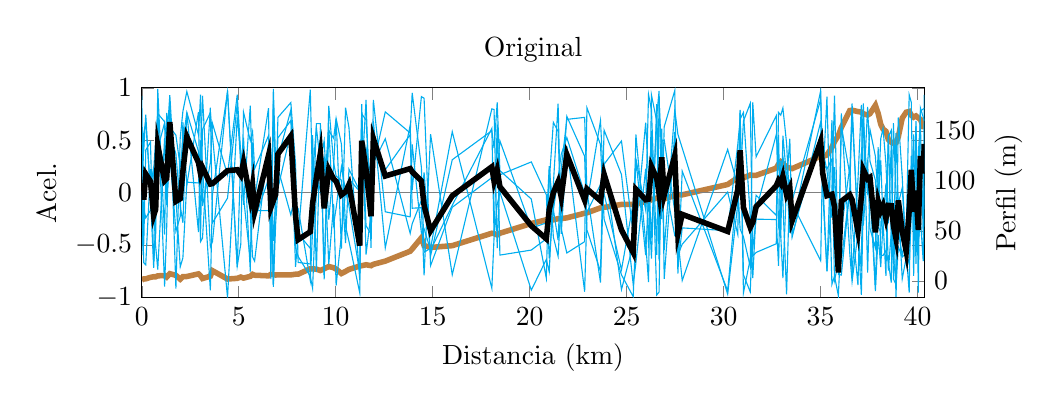
\begin{tikzpicture}
\pgfplotsset{%
    width=0.95\textwidth,
    height=0.35\textwidth
}
    \begin{axis}[
      axis y line*=right,
      axis x line=none,
      ylabel=Perfil (m),
      xmin=0,xmax=40346
    ]
    \addplot[color=brown, line width=2pt] coordinates {(0,0.87)(102.164,1.96)(203.92700000000002,2.08)(447.94500000000005,3.55)(613.325,4.17)(716.186,4.11)(823.47,5.07)(1176.592,5.38)(1282.9530000000002,3.84)(1445.4260000000002,7.25)(1759.0880000000002,5.55)(1982.15,1.73)(2119.9010000000003,4.26)(2322.943,4.41)(2924.277,7.04)(3030.437,5.18)(3130.813,2.38)(3536.143,4.74)(3644.949,10.22)(4420.9130000000005,1.9)(4921.3240000000005,2.56)(5104.733,3.87)(5245.344,2.82)(5594.861,4.54)(5710.807,6.57)(5817.772,5.68)(6534.901,5.07)(6654.088,6.53)(6783.7,6.45)(6902.016,5.91)(7020.003,5.97)(7685.297,6.03)(7928.504,6.71)(8062.249,6.71)(8688.872,12.23)(8807.58,12.11)(9002.436,11.74)(9210.017,10.43)(9403.583,12.11)(9641.305,14.38)(9892.713,13.19)(10020.635,11.84)(10293.636,7.4)(10506.469000000001,9.53)(10681.998000000001,11.49)(11237.900000000001,14.9)(11340.149000000001,15.22)(11563.322000000002,16.15)(11821.782000000003,15.26)(11939.827000000003,16.58)(12555.680000000002,19.79)(13839.171000000002,29.7)(13943.060000000001,31.97)(14416.667000000001,43.08)(14556.487000000001,35.35)(14890.702000000001,33.49)(16008.686000000002,35.26)(18050.462000000003,47.68)(18164.586000000003,47.34)(18325.663000000004,46.02)(18465.065000000002,47.71)(20084.003000000004,57.43)(20857.488000000005,61.1)(21009.720000000005,61.43)(21221.142000000003,61.07)(21465.656000000003,62.3)(21627.590000000004,62.37)(21915.516000000003,63.08)(22834.536000000004,67.72)(22952.991000000005,68.13)(23651.793000000005,73.07)(23836.670000000006,73.57)(24733.588000000007,76.53)(25338.191000000006,76.46)(25476.630000000005,76.46)(25981.370000000006,79.68)(26128.677000000007,79.76)(26280.104000000007,81.27)(26551.986000000008,82.92)(26672.823000000008,83.2)(26812.049000000006,82.04)(26937.280000000006,82.06)(27482.118000000006,85.47)(27643.210000000006,86.22)(27865.914000000008,86.13)(30208.929000000007,96.47)(30729.789000000008,103.29)(30851.175000000007,103.63)(31022.892000000007,103.08)(31373.032000000007,105.97)(31504.037000000008,105.6)(31676.333000000006,105.6)(32714.764000000006,112.78)(32831.530000000006,116.81)(32947.049000000006,119.15)(33057.22000000001,117.42)(33247.047000000006,113.82)(33414.321,113.0)(33535.26500000001,112.36)(35005.57600000001,124.81)(35109.21000000001,124.4)(35328.725000000006,126.05)(35584.062000000005,133.63)(35718.11400000001,139.43)(35917.28500000001,145.46)(36070.40500000001,153.45)(36503.86500000001,170.4)(36623.96900000001,170.76)(36926.16700000001,169.43)(37102.41000000001,168.93)(37205.05900000001,167.17)(37425.69800000001,165.97)(37546.65000000001,167.33)(37826.07800000001,175.65)(37968.48600000001,167.58)(38103.27700000001,156.65)(38220.99300000001,151.89)(38369.83800000001,149.67)(38495.22200000001,141.33)(38645.14800000001,138.8)(38754.81700000001,137.76)(38890.53500000001,138.18)(39007.28600000001,144.07)(39209.689000000006,162.84)(39413.97000000001,168.76)(39568.76400000001,169.54)(39678.03100000001,165.82)(39799.18100000001,163.8)(39916.84600000001,165.02)(40040.41400000001,163.02)(40144.534000000014,161.74)(40292.13800000001,154.38)(40345.99300000002,154.23)};
    \end{axis}
      \begin{axis}[
      title={Original},
      xlabel={Distancia (km)},
      ylabel={Acel.},
      ymin=-1,ymax=1,xmin=0,xmax=40346,
      scaled x ticks = false,
      xtick={0,5000,10000,15000,20000,25000,30000,35000,40000},
      xticklabels={0,5,10,15,20,25,30,35,40}]
      
      \addplot[color=gray] coordinates {(0,0)(40346,0)};
      
      \addplot[color=cyan] coordinates {(0,0.48303785)(102.164,0.4087189)(203.92700000000002,0.74541871)(447.94500000000005,-0.03099373)(613.325,-0.71799794)(716.186,-0.25708803)(823.47,0.82503353)(1176.592,-0.89579131)(1282.9530000000002,-0.34495415)(1445.4260000000002,0.8750705)(1759.0880000000002,-0.91393511)(1982.15,0.52156396)(2119.9010000000003,0.7759734)(2322.943,0.96535861)(2924.277,0.55244227)(3030.437,0.93556825)(3130.813,-0.12765526)(3536.143,0.28469026)(3644.949,0.66023547)(4420.9130000000005,0.1703067)(4921.3240000000005,0.93424731)(5104.733,0.35968597)(5245.344,0.31310484)(5594.861,-0.19239181)(5710.807,-0.61165505)(5817.772,-0.65262612)(6534.901,0.46799668)(6654.088,-0.68217857)(6783.7,0.98927139)(6902.016,0.30171766)(7020.003,0.32994364)(7685.297,0.78817003)(7928.504,-0.52764639)(8062.249,-0.60871957)(8688.872,-0.79791019)(8807.58,-0.91208745)(9002.436,0.00949483)(9210.017,0.29965309)(9403.583,0.49499163)(9641.305,-0.25738089)(9892.713,0.25853082)(10020.635,0.70977536)(10293.636,-0.53438638)(10506.469000000001,0.81140644)(10681.998000000001,0.62299643)(11237.900000000001,-0.83478558)(11340.149000000001,0.13924977)(11563.322000000002,0.88416122)(11821.782000000003,-0.52723948)(11939.827000000003,0.88548626)(12555.680000000002,-0.18235783)(13839.171000000002,-0.23037173)(13943.060000000001,0.45994851)(14416.667000000001,-0.38382441)(14556.487000000001,-0.34455891)(14890.702000000001,-0.54900648)(16008.686000000002,-0.1203613)(18050.462000000003,0.612956)(18164.586000000003,-0.41536831)(18325.663000000004,-0.1160324)(18465.065000000002,0.00579139)(20084.003000000004,-0.92957245)(20857.488000000005,-0.63705045)(21009.720000000005,-0.7551067)(21221.142000000003,0.07651198)(21465.656000000003,0.85066378)(21627.590000000004,-0.39170798)(21915.516000000003,0.44444547)(22834.536000000004,-0.9446756)(22952.991000000005,-0.18433026)(23651.793000000005,0.07708568)(23836.670000000006,0.27749306)(24733.588000000007,-0.92375565)(25338.191000000006,-0.49682093)(25476.630000000005,0.55522302)(25981.370000000006,-0.47370418)(26128.677000000007,-0.85345045)(26280.104000000007,0.93255504)(26551.986000000008,0.68141618)(26672.823000000008,-0.64725583)(26812.049000000006,0.50641209)(26937.280000000006,-0.54817083)(27482.118000000006,0.79232902)(27643.210000000006,0.55701787)(27865.914000000008,0.42626929)(30208.929000000007,-0.96735136)(30729.789000000008,-0.10498194)(30851.175000000007,0.78627818)(31022.892000000007,-0.956224)(31373.032000000007,-0.63227536)(31504.037000000008,-0.52795437)(31676.333000000006,-0.25251361)(32714.764000000006,-0.25616557)(32831.530000000006,-0.69695879)(32947.049000000006,0.24040537)(33057.22000000001,0.34257397)(33247.047000000006,0.15128995)(33414.321,0.10870376)(33535.26500000001,-0.42212792)(35005.57600000001,0.67604427)(35109.21000000001,0.02135457)(35328.725000000006,-0.74896034)(35584.062000000005,0.69268448)(35718.11400000001,-0.20984079)(35917.28500000001,-0.68353137)(36070.40500000001,0.63252321)(36503.86500000001,0.17895029)(36623.96900000001,0.85133016)(36926.16700000001,-0.36836149)(37102.41000000001,-0.9747614)(37205.05900000001,-0.05169141)(37425.69800000001,0.81879303)(37546.65000000001,0.29956233)(37826.07800000001,0.11954253)(37968.48600000001,-0.32615156)(38103.27700000001,-0.37677139)(38220.99300000001,-0.07464349)(38369.83800000001,-0.23595292)(38495.22200000001,0.55861449)(38645.14800000001,-0.43290058)(38754.81700000001,-0.6807297)(38890.53500000001,0.56767519)(39007.28600000001,-0.10721657)(39209.689000000006,0.04713388)(39413.97000000001,-0.56852504)(39568.76400000001,-0.95231977)(39678.03100000001,0.35347062)(39799.18100000001,-0.33703526)(39916.84600000001,0.68380121)(40040.41400000001,-0.48117133)(40144.534000000014,-0.24069175)(40292.13800000001,-0.65261272)(40345.99300000002,0.06811072)};

      \addplot[color=cyan] coordinates {(0,-0.59274191)(102.164,-0.14528758)(203.92700000000002,-0.24068932)(447.94500000000005,-0.16791346)(613.325,0.21467706)(716.186,0.49901898)(823.47,0.75529863)(1176.592,0.6768439)(1282.9530000000002,-0.11951662)(1445.4260000000002,0.379444)(1759.0880000000002,-0.36891532)(1982.15,-0.22648493)(2119.9010000000003,0.67310256)(2322.943,0.07276684)(2924.277,0.76936353)(3030.437,-0.41825488)(3130.813,0.60242682)(3536.143,0.76381237)(3644.949,0.54284343)(4420.9130000000005,-0.99986636)(4921.3240000000005,0.71768141)(5104.733,0.37535725)(5245.344,-0.04131251)(5594.861,-0.64680532)(5710.807,-0.17864765)(5817.772,-0.05562594)(6534.901,0.80562624)(6654.088,-0.82539203)(6783.7,0.87480521)(6902.016,-0.04702207)(7020.003,0.52315234)(7685.297,0.68847603)(7928.504,-0.14562016)(8062.249,-0.14917098)(8688.872,-0.83864505)(8807.58,-0.35987595)(9002.436,0.65880103)(9210.017,0.65839179)(9403.583,-0.82770375)(9641.305,0.59220696)(9892.713,0.51900331)(10020.635,0.70825577)(10293.636,0.46263747)(10506.469000000001,-0.31943709)(10681.998000000001,-0.46345787)(11237.900000000001,-0.95535035)(11340.149000000001,0.75532737)(11563.322000000002,-0.31507315)(11821.782000000003,-0.39444676)(11939.827000000003,0.26762512)(12555.680000000002,0.77100818)(13839.171000000002,0.56997802)(13943.060000000001,0.95289936)(14416.667000000001,0.2438116)(14556.487000000001,-0.5690014)(14890.702000000001,-0.52935136)(16008.686000000002,0.58174064)(18050.462000000003,-0.91192793)(18164.586000000003,-0.4256566)(18325.663000000004,0.65278729)(18465.065000000002,-0.59536079)(20084.003000000004,-0.5473516)(20857.488000000005,-0.44037591)(21009.720000000005,0.1075767)(21221.142000000003,0.67073624)(21465.656000000003,0.58452572)(21627.590000000004,-0.34320225)(21915.516000000003,-0.57518989)(22834.536000000004,-0.46703597)(22952.991000000005,0.80972828)(23651.793000000005,0.45955492)(23836.670000000006,-0.2526341)(24733.588000000007,-0.78346564)(25338.191000000006,-0.99136321)(25476.630000000005,-0.36134165)(25981.370000000006,0.66818309)(26128.677000000007,0.15100318)(26280.104000000007,-0.434307)(26551.986000000008,0.73079331)(26672.823000000008,0.97167916)(26812.049000000006,-0.25186481)(26937.280000000006,0.62833991)(27482.118000000006,0.97413411)(27643.210000000006,-0.70434095)(27865.914000000008,-0.33601152)(30208.929000000007,-0.36235265)(30729.789000000008,0.45767795)(30851.175000000007,0.70102815)(31022.892000000007,0.76508363)(31373.032000000007,-0.22349418)(31504.037000000008,-0.81586832)(31676.333000000006,-0.16612053)(32714.764000000006,0.55395382)(32831.530000000006,0.29588465)(32947.049000000006,0.3000612)(33057.22000000001,-0.09586118)(33247.047000000006,-0.9699263)(33414.321,0.12620914)(33535.26500000001,-0.10394128)(35005.57600000001,-0.648826)(35109.21000000001,0.40706684)(35328.725000000006,0.21260961)(35584.062000000005,-0.24005888)(35718.11400000001,0.24480815)(35917.28500000001,-0.77921322)(36070.40500000001,-0.78598004)(36503.86500000001,0.01736868)(36623.96900000001,-0.80105567)(36926.16700000001,0.11567844)(37102.41000000001,0.83771859)(37205.05900000001,-0.11423768)(37425.69800000001,0.31458824)(37546.65000000001,-0.34323511)(37826.07800000001,-0.52554359)(37968.48600000001,0.43436138)(38103.27700000001,-0.59452197)(38220.99300000001,-0.59956396)(38369.83800000001,-0.55149212)(38495.22200000001,-0.66340757)(38645.14800000001,-0.85826159)(38754.81700000001,0.66252413)(38890.53500000001,-0.01756387)(39007.28600000001,-0.36761136)(39209.689000000006,-0.59692385)(39413.97000000001,-0.41138132)(39568.76400000001,0.93417731)(39678.03100000001,0.8615691)(39799.18100000001,-0.79317661)(39916.84600000001,0.6356446)(40040.41400000001,-0.95231825)(40144.534000000014,0.80974066)(40292.13800000001,0.72041618)(40345.99300000002,0.68327376)};

      \addplot[color=cyan] coordinates {(0,-0.34197357)(102.164,0.56617521)(203.92700000000002,0.67118318)(447.94500000000005,0.03064361)(613.325,0.24986647)(716.186,-0.11327734)(823.47,0.41903722)(1176.592,0.66768126)(1282.9530000000002,0.48478912)(1445.4260000000002,0.93167034)(1759.0880000000002,-0.0487421)(1982.15,-0.70814416)(2119.9010000000003,-0.62197777)(2322.943,0.10040061)(2924.277,0.0929481)(3030.437,0.35164992)(3130.813,0.92463586)(3536.143,-0.51647102)(3644.949,-0.46767013)(4420.9130000000005,0.97335304)(4921.3240000000005,-0.70067747)(5104.733,-0.49191192)(5245.344,0.76854776)(5594.861,0.49722803)(5710.807,0.58445327)(5817.772,0.22855251)(6534.901,0.54433549)(6654.088,0.06022494)(6783.7,-0.88258743)(6902.016,0.05740292)(7020.003,0.23089264)(7685.297,-0.21252035)(7928.504,-0.00435776)(8062.249,-0.42613983)(8688.872,0.98370449)(8807.58,0.04638707)(9002.436,0.17333724)(9210.017,0.01488617)(9403.583,0.34761647)(9641.305,-0.68391898)(9892.713,-0.10645207)(10020.635,-0.88523386)(10293.636,-0.40160863)(10506.469000000001,0.01361528)(10681.998000000001,-0.12510632)(11237.900000000001,-0.76468386)(11340.149000000001,0.84539893)(11563.322000000002,-0.58945287)(11821.782000000003,-0.19782691)(11939.827000000003,0.28336357)(12555.680000000002,0.51407733)(13839.171000000002,-0.38786406)(13943.060000000001,-0.29652213)(14416.667000000001,-0.07301677)(14556.487000000001,0.1943334)(14890.702000000001,-0.60311386)(16008.686000000002,0.3144765)(18050.462000000003,0.59145895)(18164.586000000003,0.42490603)(18325.663000000004,0.86151142)(18465.065000000002,0.21119295)(20084.003000000004,-0.06076554)(20857.488000000005,-0.81451488)(21009.720000000005,0.22899959)(21221.142000000003,-0.16670623)(21465.656000000003,0.14330505)(21627.590000000004,0.36513222)(21915.516000000003,0.52558514)(22834.536000000004,-0.00699043)(22952.991000000005,-0.10063818)(23651.793000000005,0.68747528)(23836.670000000006,-0.01008918)(24733.588000000007,-0.73499234)(25338.191000000006,-0.10065325)(25476.630000000005,0.32198598)(25981.370000000006,-0.16505104)(26128.677000000007,0.93727176)(26280.104000000007,0.79253497)(26551.986000000008,-0.59209612)(26672.823000000008,0.88114147)(26812.049000000006,0.33177353)(26937.280000000006,0.12855694)(27482.118000000006,-0.40967113)(27643.210000000006,-0.44178132)(27865.914000000008,-0.83796395)(30208.929000000007,0.41277721)(30729.789000000008,0.06689429)(30851.175000000007,-0.34592222)(31022.892000000007,-0.4201353)(31373.032000000007,-0.70607539)(31504.037000000008,0.86146625)(31676.333000000006,0.34263771)(32714.764000000006,0.73385394)(32831.530000000006,-0.32754849)(32947.049000000006,-0.41537926)(33057.22000000001,-0.8138985)(33247.047000000006,0.09306588)(33414.321,0.51437628)(33535.26500000001,-0.40032678)(35005.57600000001,0.56053393)(35109.21000000001,0.14152728)(35328.725000000006,-0.74927221)(35584.062000000005,0.0256756)(35718.11400000001,0.92491217)(35917.28500000001,-0.69249804)(36070.40500000001,0.75629407)(36503.86500000001,-0.57513153)(36623.96900000001,-0.84940186)(36926.16700000001,-0.38729232)(37102.41000000001,0.38403687)(37205.05900000001,-0.31361863)(37425.69800000001,0.28048282)(37546.65000000001,0.60340268)(37826.07800000001,0.34735621)(37968.48600000001,-0.06211883)(38103.27700000001,0.30724329)(38220.99300000001,-0.27647661)(38369.83800000001,-0.79383954)(38495.22200000001,0.5348295)(38645.14800000001,0.59497459)(38754.81700000001,-0.59644243)(38890.53500000001,-0.8713408)(39007.28600000001,0.71711391)(39209.689000000006,0.15293107)(39413.97000000001,-0.62116319)(39568.76400000001,0.03609342)(39678.03100000001,-0.16849242)(39799.18100000001,-0.20417382)(39916.84600000001,-0.06068636)(40040.41400000001,-0.31532511)(40144.534000000014,-0.28289788)(40292.13800000001,0.45914458)(40345.99300000002,-0.159819)};

      \addplot[color=cyan] coordinates{(0,-0.02113317)(102.164,-0.66789852)(203.92700000000002,-0.68851134)(447.94500000000005,0.22563936)(613.325,-0.17539174)(716.186,-0.50910004)(823.47,-0.732599)(1176.592,0.52026106)(1282.9530000000002,-0.10621095)(1445.4260000000002,0.62347941)(1759.0880000000002,0.54894352)(1982.15,0.24840298)(2119.9010000000003,0.48519916)(2322.943,0.76606462)(2924.277,0.392752)(3030.437,-0.46688815)(3130.813,-0.43351482)(3536.143,0.81233486)(3644.949,-0.28725966)(4420.9130000000005,-0.05194502)(4921.3240000000005,0.84993756)(5104.733,0.2469896)(5245.344,0.52403114)(5594.861,-0.75263984)(5710.807,0.47881994)(5817.772,-0.17097581)(6534.901,-0.17062673)(6654.088,0.42762306)(6783.7,-0.46014078)(6902.016,-0.09045009)(7020.003,0.71827767)(7685.297,0.85964187)(7928.504,0.27685171)(8062.249,-0.66548419)(8688.872,-0.68021583)(8807.58,0.54856629)(9002.436,-0.75562419)(9210.017,0.62248585)(9403.583,-0.78515574)(9641.305,0.82805744)(9892.713,0.28567909)(10020.635,0.15840646)(10293.636,0.11972202)(10506.469000000001,-0.48097392)(10681.998000000001,0.22268881)(11237.900000000001,0.01864109)(11340.149000000001,0.75295095)(11563.322000000002,0.69253598)(11821.782000000003,-0.15163444)(11939.827000000003,0.46737294)(12555.680000000002,0.2195683)(13839.171000000002,0.55389023)(13943.060000000001,-0.1482953)(14416.667000000001,-0.14275528)(14556.487000000001,-0.78888972)(14890.702000000001,0.55803137)(16008.686000000002,-0.78255029)(18050.462000000003,0.79987193)(18164.586000000003,0.79357076)(18325.663000000004,-0.52925998)(18465.065000000002,0.17048773)(20084.003000000004,0.29354434)(20857.488000000005,-0.01855385)(21009.720000000005,-0.62728841)(21221.142000000003,-0.15854215)(21465.656000000003,-0.45267528)(21627.590000000004,0.22937175)(21915.516000000003,0.69932578)(22834.536000000004,0.7186574)(22952.991000000005,0.01236223)(23651.793000000005,-0.85653589)(23836.670000000006,0.27087928)(24733.588000000007,0.49300993)(25338.191000000006,-0.38646688)(25476.630000000005,0.31908781)(25981.370000000006,-0.59636805)(26128.677000000007,-0.0150497)(26280.104000000007,-0.62912071)(26551.986000000008,0.84452178)(26672.823000000008,-0.31436471)(26812.049000000006,0.49105715)(26937.280000000006,0.50333276)(27482.118000000006,-0.17582334)(27643.210000000006,-0.59267291)(27865.914000000008,-0.49189229)(30208.929000000007,0.00618446)(30729.789000000008,-0.39745333)(30851.175000000007,0.78884613)(31022.892000000007,-0.78293876)(31373.032000000007,-0.94632826)(31504.037000000008,-0.33533241)(31676.333000000006,-0.02444096)(32714.764000000006,-0.21543707)(32831.530000000006,0.5505653)(32947.049000000006,-0.43337645)(33057.22000000001,0.54501394)(33247.047000000006,0.15659161)(33414.321,-0.3822164)(33535.26500000001,-0.07375459)(35005.57600000001,0.88980755)(35109.21000000001,0.2800682)(35328.725000000006,0.22530821)(35584.062000000005,0.32086431)(35718.11400000001,-0.83608509)(35917.28500000001,-0.67172844)(36070.40500000001,-0.65046786)(36503.86500000001,0.03198747)(36623.96900000001,0.75795051)(36926.16700000001,-0.32218554)(37102.41000000001,-0.74816421)(37205.05900000001,0.72110544)(37425.69800000001,0.00845562)(37546.65000000001,0.14689627)(37826.07800000001,-0.89440203)(37968.48600000001,-0.04441946)(38103.27700000001,0.51503105)(38220.99300000001,0.61350306)(38369.83800000001,0.27393879)(38495.22200000001,-0.29224592)(38645.14800000001,0.45879402)(38754.81700000001,-0.82300108)(38890.53500000001,-0.87698267)(39007.28600000001,-0.51650237)(39209.689000000006,-0.61228067)(39413.97000000001,-0.58031408)(39568.76400000001,-0.67843922)(39678.03100000001,-0.20785475)(39799.18100000001,0.55694411)(39916.84600000001,-0.67858219)(40040.41400000001,0.37156035)(40144.534000000014,0.68335453)(40292.13800000001,-0.40587593)(40345.99300000002,0.9324516)};

      \addplot[color=cyan] coordinates {(0,0.923804948)(102.164,-0.492857123)(203.92700000000002,0.405488224)(447.94500000000005,0.483062941)(613.325,-0.655466716)(716.186,-0.409103612)(823.47,0.990132771)(1176.592,-0.398701844)(1282.9530000000002,0.761368685)(1445.4260000000002,0.555998174)(1759.0880000000002,0.370929029)(1982.15,-0.122577200)(2119.9010000000003,-0.286682308)(2322.943,0.765913677)(2924.277,-0.376025505)(3030.437,0.497837921)(3130.813,0.240089215)(3536.143,-0.931515963)(3644.949,-0.0142403361)(4420.9130000000005,0.960459745)(4921.3240000000005,-0.707629406)(5104.733,0.347281865)(5245.344,-0.114721099)(5594.861,0.830949335)(5710.807,0.0973305497)(5817.772,-0.256853242)(6534.901,0.129526991)(6654.088,0.309330415)(6783.7,-0.898944419)(6902.016,-0.301405476)(7020.003,0.0427493723)(7685.297,0.576925214)(7928.504,-0.708005519)(8062.249,-0.391340493)(8688.872,-0.530915233)(8807.58,0.163901658)(9002.436,0.622075501)(9210.017,0.283157102)(9403.583,0.0220229541)(9641.305,0.630201217)(9892.713,-0.300269898)(10020.635,-0.147001943)(10293.636,0.247552802)(10506.469000000001,0.0201119927)(10681.998000000001,0.130081006)(11237.900000000001,0.0116594942)(11340.149000000001,-0.0146305513)(11563.322000000002,0.428960696)(11821.782000000003,0.146723442)(11939.827000000003,0.682973810)(12555.680000000002,-0.526204542)(13839.171000000002,0.643025623)(13943.060000000001,0.0277462904)(14416.667000000001,0.916878202)(14556.487000000001,0.901311016)(14890.702000000001,-0.695547134)(16008.686000000002,-0.138820471)(18050.462000000003,0.143321035)(18164.586000000003,0.165402128)(18325.663000000004,0.209673223)(18465.065000000002,0.494639280)(20084.003000000004,-0.337486962)(20857.488000000005,-0.288604502)(21009.720000000005,0.252252842)(21221.142000000003,-0.422075047)(21465.656000000003,-0.606115462)(21627.590000000004,-0.0656440617)(21915.516000000003,0.728612545)(22834.536000000004,0.347023446)(22952.991000000005,-0.354628861)(23651.793000000005,-0.750767541)(23836.670000000006,0.597182077)(24733.588000000007,0.173434826)(25338.191000000006,-0.876209737)(25476.630000000005,-0.671016511)(25981.370000000006,0.229943884)(26128.677000000007,-0.530559279)(26280.104000000007,0.588616770)(26551.986000000008,-0.975567339)(26672.823000000008,-0.947799495)(26812.049000000006,0.610619164)(26937.280000000006,-0.822244073)(27482.118000000006,0.580488060)(27643.210000000006,-0.772149844)(27865.914000000008,0.205688647)(30208.929000000007,-0.937424826)(30729.789000000008,0.121867587)(30851.175000000007,0.0936886434)(31022.892000000007,0.683176557)(31373.032000000007,0.851348116)(31504.037000000008,-0.605478723)(31676.333000000006,-0.569968267)(32714.764000000006,-0.487382151)(32831.530000000006,0.765911934)(32947.049000000006,0.739949368)(33057.22000000001,0.807983796)(33247.047000000006,0.471330727)(33414.321,-0.138651863)(33535.26500000001,-0.328791263)(35005.57600000001,0.973125379)(35109.21000000001,0.0812108919)(35328.725000000006,0.917051819)(35584.062000000005,-0.873888770)(35718.11400000001,-0.796623641)(35917.28500000001,-0.981804283)(36070.40500000001,-0.359159031)(36503.86500000001,0.243641112)(36623.96900000001,-0.293279198)(36926.16700000001,-0.880520187)(37102.41000000001,0.311919409)(37205.05900000001,0.852917315)(37425.69800000001,-0.762846507)(37546.65000000001,0.0241828648)(37826.07800000001,-0.938377321)(37968.48600000001,-0.402928202)(38103.27700000001,-0.709179609)(38220.99300000001,-0.273848880)(38369.83800000001,0.0873809222)(38495.22200000001,-0.743785874)(38645.14800000001,-0.382462939)(38754.81700000001,-0.130057005)(38890.53500000001,-0.992684022)(39007.28600000001,-0.0946969088)(39209.689000000006,-0.821743543)(39413.97000000001,-0.620516629)(39568.76400000001,-0.166740173)(39678.03100000001,0.258491058)(39799.18100000001,-0.123215892)(39916.84600000001,-0.481429811)(40040.41400000001,-0.406253180)(40144.534000000014,0.778759337)(40292.13800000001,0.798484810)(40345.99300000002,0.803791423)};
        
    \addplot[color=black, line width=2pt] coordinates {(0,0.0901988316)(102.164,-0.0662298226)(203.92700000000002,0.1785778908)(447.94500000000005,0.1080877442)(613.325,-0.2168625732)(716.186,-0.1579100084)(823.47,0.4513806302)(1176.592,0.1140586132)(1282.9530000000002,0.135095217)(1445.4260000000002,0.6731324848)(1759.0880000000002,-0.0823439962)(1982.15,-0.05744787)(2119.9010000000003,0.2051230084)(2322.943,0.5341008714)(2924.277,0.286296079)(3030.437,0.1799826122)(3130.813,0.241196363)(3536.143,0.0825701014)(3644.949,0.08678175478)(4420.9130000000005,0.210461621)(4921.3240000000005,0.2187118808)(5104.733,0.167480553)(5245.344,0.2899300262)(5594.861,-0.052731921)(5710.807,0.07406021194)(5817.772,-0.1815057204)(6534.901,0.3553717342)(6654.088,-0.142078437)(6783.7,-0.0755192058)(6902.016,-0.0159514112)(7020.003,0.36900313246)(7685.297,0.5401385588)(7928.504,-0.2217556238)(8062.249,-0.4481710126)(8688.872,-0.3727963626)(8807.58,-0.1026216764)(9002.436,0.1416168822)(9210.017,0.3757148004)(9403.583,-0.14964568718)(9641.305,0.2218331494)(9892.713,0.1312982504)(10020.635,0.1088403574)(10293.636,-0.0212165436)(10506.469000000001,0.00894454054)(10681.998000000001,0.0774404112)(11237.900000000001,-0.50490384116)(11340.149000000001,0.49565929374)(11563.322000000002,0.2202263752)(11821.782000000003,-0.2248848296)(11939.827000000003,0.51736434)(12555.680000000002,0.1592182876)(13839.171000000002,0.2297316166)(13943.060000000001,0.19915534608)(14416.667000000001,0.1122186684)(14556.487000000001,-0.1213611228)(14890.702000000001,-0.3637974928)(16008.686000000002,-0.0291029842)(18050.462000000003,0.247135997)(18164.586000000003,0.1085708016)(18325.663000000004,0.2157359106)(18465.065000000002,0.057350112)(20084.003000000004,-0.3163264424)(20857.488000000005,-0.4398199184)(21009.720000000005,-0.1587131956)(21221.142000000003,-1.50414000000043E-05)(21465.656000000003,0.1039407616)(21627.590000000004,-0.04121006434)(21915.516000000003,0.364555809)(22834.536000000004,-0.0706042308)(22952.991000000005,0.0364986418)(23651.793000000005,-0.0766375102)(23836.670000000006,0.1765662274)(24733.588000000007,-0.3551537748)(25338.191000000006,-0.5703028014)(25476.630000000005,0.0327877298)(25981.370000000006,-0.0673992592)(26128.677000000007,-0.0621568978)(26280.104000000007,0.250055814)(26551.986000000008,0.1378135622)(26672.823000000008,-0.011319881)(26812.049000000006,0.3375994248)(26937.280000000006,-0.0220370586)(27482.118000000006,0.352291344)(27643.210000000006,-0.3907854308)(27865.914000000008,-0.2067819646)(30208.929000000007,-0.3696334332)(30729.789000000008,0.0288009114)(30851.175000000007,0.40478377668)(31022.892000000007,-0.1422075746)(31373.032000000007,-0.3313650148)(31504.037000000008,-0.2846335146)(31676.333000000006,-0.1340811314)(32714.764000000006,0.0657645938)(32831.530000000006,0.1175709208)(32947.049000000006,0.0863320456)(33057.22000000001,0.1571624052)(33247.047000000006,-0.0195296266)(33414.321,0.0456841834)(33535.26500000001,-0.2657883666)(35005.57600000001,0.4901370258)(35109.21000000001,0.18624555638)(35328.725000000006,-0.0286525822)(35584.062000000005,-0.014944652)(35718.11400000001,-0.1345658402)(35917.28500000001,-0.7617550706)(36070.40500000001,-0.0813579302)(36503.86500000001,-0.0206367956)(36623.96900000001,-0.0668912116)(36926.16700000001,-0.3685362194)(37102.41000000001,-0.0378501482)(37205.05900000001,0.218895007)(37425.69800000001,0.1318946406)(37546.65000000001,0.14616180696)(37826.07800000001,-0.3782848402)(37968.48600000001,-0.0802513344)(38103.27700000001,-0.1716397258)(38220.99300000001,-0.122205976)(38369.83800000001,-0.24399297356)(38495.22200000001,-0.1211990748)(38645.14800000001,-0.1239712998)(38754.81700000001,-0.313541217)(38890.53500000001,-0.4381792344)(39007.28600000001,-0.07378265976)(39209.689000000006,-0.3661766226)(39413.97000000001,-0.5603800518)(39568.76400000001,-0.1654456866)(39678.03100000001,0.2194367216)(39799.18100000001,-0.1801314944)(39916.84600000001,0.0197494898)(40040.41400000001,-0.356701504)(40144.534000000014,0.3496529794)(40292.13800000001,0.183911384)(40345.99300000002,0.4655617006)};
      \end{axis}
       
\end{tikzpicture}
\end{subfigure}
% FIGURE 38
\begin{subfigure}[b]{\textwidth}
\centering
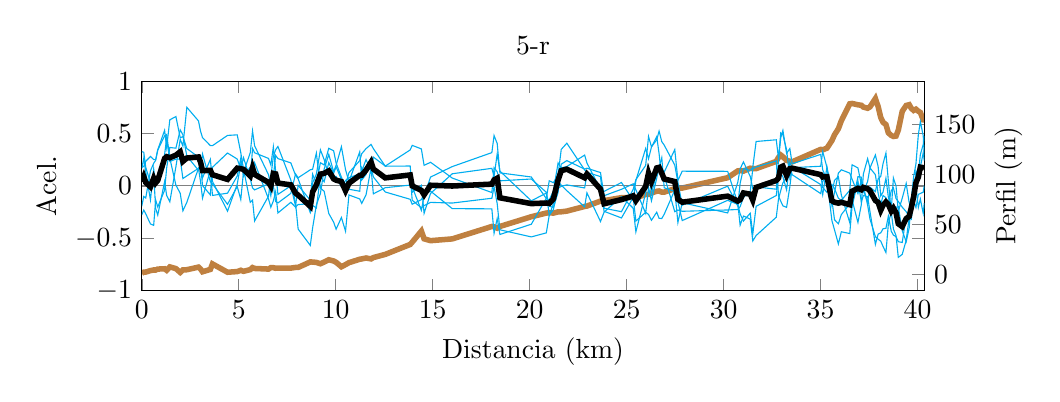
\begin{tikzpicture}
\pgfplotsset{%
    width=0.95\textwidth,
    height=0.35\textwidth
}
     \begin{axis}[
      axis y line*=right,
      axis x line=none,
      ylabel=Perfil (m),
      xmin=0,xmax=40346
    ]
    \addplot[color=brown, line width=2pt] coordinates {(0,0.87)(102.164,1.96)(203.92700000000002,2.08)(447.94500000000005,3.55)(613.325,4.17)(716.186,4.11)(823.47,5.07)(1176.592,5.38)(1282.9530000000002,3.84)(1445.4260000000002,7.25)(1759.0880000000002,5.55)(1982.15,1.73)(2119.9010000000003,4.26)(2322.943,4.41)(2924.277,7.04)(3030.437,5.18)(3130.813,2.38)(3536.143,4.74)(3644.949,10.22)(4420.9130000000005,1.9)(4921.3240000000005,2.56)(5104.733,3.87)(5245.344,2.82)(5594.861,4.54)(5710.807,6.57)(5817.772,5.68)(6534.901,5.07)(6654.088,6.53)(6783.7,6.45)(6902.016,5.91)(7020.003,5.97)(7685.297,6.03)(7928.504,6.71)(8062.249,6.71)(8688.872,12.23)(8807.58,12.11)(9002.436,11.74)(9210.017,10.43)(9403.583,12.11)(9641.305,14.38)(9892.713,13.19)(10020.635,11.84)(10293.636,7.4)(10506.469000000001,9.53)(10681.998000000001,11.49)(11237.900000000001,14.9)(11340.149000000001,15.22)(11563.322000000002,16.15)(11821.782000000003,15.26)(11939.827000000003,16.58)(12555.680000000002,19.79)(13839.171000000002,29.7)(13943.060000000001,31.97)(14416.667000000001,43.08)(14556.487000000001,35.35)(14890.702000000001,33.49)(16008.686000000002,35.26)(18050.462000000003,47.68)(18164.586000000003,47.34)(18325.663000000004,46.02)(18465.065000000002,47.71)(20084.003000000004,57.43)(20857.488000000005,61.1)(21009.720000000005,61.43)(21221.142000000003,61.07)(21465.656000000003,62.3)(21627.590000000004,62.37)(21915.516000000003,63.08)(22834.536000000004,67.72)(22952.991000000005,68.13)(23651.793000000005,73.07)(23836.670000000006,73.57)(24733.588000000007,76.53)(25338.191000000006,76.46)(25476.630000000005,76.46)(25981.370000000006,79.68)(26128.677000000007,79.76)(26280.104000000007,81.27)(26551.986000000008,82.92)(26672.823000000008,83.2)(26812.049000000006,82.04)(26937.280000000006,82.06)(27482.118000000006,85.47)(27643.210000000006,86.22)(27865.914000000008,86.13)(30208.929000000007,96.47)(30729.789000000008,103.29)(30851.175000000007,103.63)(31022.892000000007,103.08)(31373.032000000007,105.97)(31504.037000000008,105.6)(31676.333000000006,105.6)(32714.764000000006,112.78)(32831.530000000006,116.81)(32947.049000000006,119.15)(33057.22000000001,117.42)(33247.047000000006,113.82)(33414.321,113.0)(33535.26500000001,112.36)(35005.57600000001,124.81)(35109.21000000001,124.4)(35328.725000000006,126.05)(35584.062000000005,133.63)(35718.11400000001,139.43)(35917.28500000001,145.46)(36070.40500000001,153.45)(36503.86500000001,170.4)(36623.96900000001,170.76)(36926.16700000001,169.43)(37102.41000000001,168.93)(37205.05900000001,167.17)(37425.69800000001,165.97)(37546.65000000001,167.33)(37826.07800000001,175.65)(37968.48600000001,167.58)(38103.27700000001,156.65)(38220.99300000001,151.89)(38369.83800000001,149.67)(38495.22200000001,141.33)(38645.14800000001,138.8)(38754.81700000001,137.76)(38890.53500000001,138.18)(39007.28600000001,144.07)(39209.689000000006,162.84)(39413.97000000001,168.76)(39568.76400000001,169.54)(39678.03100000001,165.82)(39799.18100000001,163.8)(39916.84600000001,165.02)(40040.41400000001,163.02)(40144.534000000014,161.74)(40292.13800000001,154.38)(40345.99300000002,154.23)};
    \end{axis}
      \begin{axis}[
      title={5-r},
      xlabel={Distancia (km)},
      ylabel={Acel.},
      ymin=-1,ymax=1,xmin=0,xmax=40346,
      scaled x ticks = false,
      xtick={0,5000,10000,15000,20000,25000,30000,35000,40000},
      xticklabels={0,5,10,15,20,25,30,35,40}]
      
      \addplot[color=gray] coordinates {(0,0)(40346,0)};
      
      \addplot[color=cyan] coordinates {(0,-0.1938196)(102.164,-0.10041567)(203.92700000000002,-0.11528936)(447.94500000000005,0.14409555)(613.325,0.21613233)(716.186,0.24476319)(823.47,0.34521723)(1176.592,0.5302811)(1282.9530000000002,0.3675395)(1445.4260000000002,0.63071348)(1759.0880000000002,0.66188262)(1982.15,0.45991292)(2119.9010000000003,0.47026081)(2322.943,0.35694891)(2924.277,0.27439452)(3030.437,0.16823361)(3130.813,0.3046684)(3536.143,0.04094474)(3644.949,0.01954292)(4420.9130000000005,-0.17526349)(4921.3240000000005,-0.00544876)(5104.733,-0.12925828)(5245.344,0.13593658)(5594.861,0.06772831)(5710.807,0.3572766)(5817.772,0.31628853)(6534.901,0.26240917)(6654.088,0.20023721)(6783.7,0.37173916)(6902.016,0.14078692)(7020.003,-0.08094336)(7685.297,0.0015198)(7928.504,-0.19235709)(8062.249,0.00613291)(8688.872,-0.13661002)(8807.58,0.11167688)(9002.436,0.02066809)(9210.017,0.22170375)(9403.583,0.19987879)(9641.305,0.35922964)(9892.713,0.33585882)(10020.635,0.21739068)(10293.636,0.08314475)(10506.469000000001,-0.00875858)(10681.998000000001,-0.03163079)(11237.900000000001,-0.0505734)(11340.149000000001,0.17544112)(11563.322000000002,0.12460884)(11821.782000000003,0.18422005)(11939.827000000003,0.0855658)(12555.680000000002,-0.05795887)(13839.171000000002,-0.12736418)(13943.060000000001,-0.17483622)(14416.667000000001,-0.13103523)(14556.487000000001,-0.07955541)(14890.702000000001,-0.04961404)(16008.686000000002,-0.21651274)(18050.462000000003,-0.21864587)(18164.586000000003,-0.45080869)(18325.663000000004,-0.31114363)(18465.065000000002,-0.46294896)(20084.003000000004,-0.36554901)(20857.488000000005,-0.11846092)(21009.720000000005,0.04931457)(21221.142000000003,0.03035835)(21465.656000000003,0.10422241)(21627.590000000004,0.34843531)(21915.516000000003,0.40745064)(22834.536000000004,0.15291808)(22952.991000000005,0.1303397)(23651.793000000005,0.08886839)(23836.670000000006,-0.21304556)(24733.588000000007,-0.24579585)(25338.191000000006,-0.03261559)(25476.630000000005,0.05974295)(25981.370000000006,0.1954947)(26128.677000000007,0.47165886)(26280.104000000007,0.37331334)(26551.986000000008,0.44017557)(26672.823000000008,0.52297241)(26812.049000000006,0.4224782)(26937.280000000006,0.38936149)(27482.118000000006,0.19886427)(27643.210000000006,0.0366666)(27865.914000000008,-0.18395153)(30208.929000000007,-0.00212205)(30729.789000000008,-0.19161683)(30851.175000000007,0.02389803)(31022.892000000007,0.1662136)(31373.032000000007,0.14722896)(31504.037000000008,0.17747839)(31676.333000000006,0.42393926)(32714.764000000006,0.44021322)(32831.530000000006,0.26194235)(32947.049000000006,0.50631733)(33057.22000000001,0.48851313)(33247.047000000006,0.34449711)(33414.321,0.07933187)(33535.26500000001,0.17247466)(35005.57600000001,0.10974691)(35109.21000000001,-0.0150245)(35328.725000000006,-0.06105663)(35584.062000000005,0.0138192)(35718.11400000001,-0.02601274)(35917.28500000001,-0.11710321)(36070.40500000001,-0.13802569)(36503.86500000001,-0.04105112)(36623.96900000001,0.20174249)(36926.16700000001,0.17186685)(37102.41000000001,0.01153626)(37205.05900000001,0.00263894)(37425.69800000001,-0.18332622)(37546.65000000001,-0.31528735)(37826.07800000001,-0.48426479)(37968.48600000001,-0.50792283)(38103.27700000001,-0.52711476)(38220.99300000001,-0.57803211)(38369.83800000001,-0.63488483)(38495.22200000001,-0.36156511)(38645.14800000001,-0.24496402)(38754.81700000001,-0.23700344)(38890.53500000001,-0.2023593)(39007.28600000001,-0.19886844)(39209.689000000006,-0.42726986)(39413.97000000001,-0.53189899)(39568.76400000001,-0.40098828)(39678.03100000001,-0.12471727)(39799.18100000001,0.08980349)(39916.84600000001,0.21011964)(40040.41400000001,0.48822656)(40144.534000000014,0.61300088)(40292.13800000001,0.47899837)(40345.99300000002,0.28868447)};

      \addplot[color=cyan] coordinates {(0,0.3274351)(102.164,0.32123635)(203.92700000000002,0.17763676)(447.94500000000005,0.02961158)(613.325,0.11287451)(716.186,-0.2153675)(823.47,-0.27815958)(1176.592,0.04045411)(1282.9530000000002,-0.09091531)(1445.4260000000002,-0.15160922)(1759.0880000000002,0.18274372)(1982.15,0.44480627)(2119.9010000000003,0.38028063)(2322.943,0.7501813)(2924.277,0.62033745)(3030.437,0.52208083)(3130.813,0.4610562)(3536.143,0.38462908)(3644.949,0.3843649)(4420.9130000000005,0.48183314)(4921.3240000000005,0.48751606)(5104.733,0.3169906)(5245.344,0.16059825)(5594.861,-0.15677643)(5710.807,-0.13511429)(5817.772,-0.33417098)(6534.901,-0.09783834)(6654.088,0.08483621)(6783.7,0.28135016)(6902.016,0.34538483)(7020.003,0.37629126)(7685.297,0.05669307)(7928.504,-0.1632325)(8062.249,-0.41163872)(8688.872,-0.56737376)(8807.58,-0.40191386)(9002.436,-0.18117162)(9210.017,-0.07306576)(9403.583,0.1610579)(9641.305,0.301114)(9892.713,0.13430611)(10020.635,0.19758907)(10293.636,0.37366453)(10506.469000000001,0.15500125)(10681.998000000001,0.04089614)(11237.900000000001,0.32460566)(11340.149000000001,0.05687647)(11563.322000000002,0.10937444)(11821.782000000003,0.23985999)(11939.827000000003,0.16593569)(12555.680000000002,0.08109315)(13839.171000000002,0.10977616)(13943.060000000001,-0.13623287)(14416.667000000001,-0.2095626)(14556.487000000001,-0.18756052)(14890.702000000001,-0.15695902)(16008.686000000002,-0.1632678)(18050.462000000003,-0.1175625)(18164.586000000003,-0.00660292)(18325.663000000004,-0.16844515)(18465.065000000002,-0.41844644)(20084.003000000004,-0.48639412)(20857.488000000005,-0.44788525)(21009.720000000005,-0.27891077)(21221.142000000003,-0.17133788)(21465.656000000003,0.04496131)(21627.590000000004,0.00704753)(21915.516000000003,-0.04512092)(22834.536000000004,-0.19983654)(22952.991000000005,-0.06599633)(23651.793000000005,-0.33963655)(23836.670000000006,-0.25006562)(24733.588000000007,-0.10215496)(25338.191000000006,-0.21231293)(25476.630000000005,-0.43850164)(25981.370000000006,-0.0672395)(26128.677000000007,0.16840792)(26280.104000000007,-0.07208785)(26551.986000000008,0.12393541)(26672.823000000008,0.18499133)(26812.049000000006,0.15694613)(26937.280000000006,0.13206646)(27482.118000000006,0.34677149)(27643.210000000006,0.0520188)(27865.914000000008,0.14065658)(30208.929000000007,0.13944641)(30729.789000000008,-0.16320197)(30851.175000000007,-0.3749109)(31022.892000000007,-0.2870315)(31373.032000000007,-0.31653783)(31504.037000000008,-0.52502658)(31676.333000000006,-0.47317354)(32714.764000000006,-0.2986374)(32831.530000000006,-0.12453173)(32947.049000000006,-0.04377102)(33057.22000000001,0.02920285)(33247.047000000006,0.08416903)(33414.321,0.17129681)(33535.26500000001,0.10705293)(35005.57600000001,-0.07299713)(35109.21000000001,0.04379901)(35328.725000000006,0.08625644)(35584.062000000005,-0.18565869)(35718.11400000001,-0.06342496)(35917.28500000001,0.12215716)(36070.40500000001,0.1538863)(36503.86500000001,0.12218216)(36623.96900000001,0.06393615)(36926.16700000001,-0.07290677)(37102.41000000001,0.05506178)(37205.05900000001,-0.05529179)(37425.69800000001,0.04228902)(37546.65000000001,0.17201098)(37826.07800000001,0.10699499)(37968.48600000001,-0.07169232)(38103.27700000001,-0.17879537)(38220.99300000001,-0.09098097)(38369.83800000001,-0.11233078)(38495.22200000001,-0.17312244)(38645.14800000001,-0.0446587)(38754.81700000001,-0.01891144)(38890.53500000001,-0.12120756)(39007.28600000001,-0.14833245)(39209.689000000006,-0.20265046)(39413.97000000001,-0.24549138)(39568.76400000001,-0.29145511)(39678.03100000001,-0.16412165)(39799.18100000001,-0.14665091)(39916.84600000001,-0.0043253)(40040.41400000001,-0.20554197)(40144.534000000014,-0.12451277)(40292.13800000001,-0.26127302)(40345.99300000002,-0.16503875)};

      \addplot[color=cyan] coordinates {(0,0.16728721)(102.164,0.2638998)(203.92700000000002,0.13280645)(447.94500000000005,-0.13377526)(613.325,0.16282272)(716.186,0.00198471)(823.47,0.05764586)(1176.592,0.29993883)(1282.9530000000002,0.45594536)(1445.4260000000002,0.23340337)(1759.0880000000002,0.25580728)(1982.15,0.25671627)(2119.9010000000003,0.07031154)(2322.943,0.09569332)(2924.277,0.1682266)(3030.437,0.03925987)(3130.813,-0.11677093)(3536.143,0.15052612)(3644.949,-0.09056735)(4420.9130000000005,-0.06912882)(4921.3240000000005,0.09423015)(5104.733,0.26326809)(5245.344,0.09064225)(5594.861,0.18079748)(5710.807,0.13724651)(5817.772,0.22205681)(6534.901,-0.12392194)(6654.088,-0.20366915)(6783.7,-0.14374862)(6902.016,-0.05426898)(7020.003,-0.25773617)(7685.297,-0.15621538)(7928.504,-0.20211733)(8062.249,-0.17788687)(8688.872,-0.16885682)(8807.58,0.02937571)(9002.436,0.1120484)(9210.017,0.34427169)(9403.583,0.25143738)(9641.305,0.09762189)(9892.713,0.09050103)(10020.635,0.09011883)(10293.636,-0.00990521)(10506.469000000001,0.05248067)(10681.998000000001,0.07895495)(11237.900000000001,0.11523653)(11340.149000000001,0.14055882)(11563.322000000002,0.25113738)(11821.782000000003,0.14356457)(11939.827000000003,0.27509581)(12555.680000000002,0.18935916)(13839.171000000002,0.34339011)(13943.060000000001,0.38705755)(14416.667000000001,0.35318903)(14556.487000000001,0.19681982)(14890.702000000001,0.22542853)(16008.686000000002,0.07513331)(18050.462000000003,-0.06319424)(18164.586000000003,0.17484304)(18325.663000000004,0.13510974)(18465.065000000002,0.04872463)(20084.003000000004,0.06609478)(20857.488000000005,-0.06025488)(21009.720000000005,-0.28040583)(21221.142000000003,-0.22603725)(21465.656000000003,-0.02259384)(21627.590000000004,-0.00363972)(21915.516000000003,0.00984952)(22834.536000000004,-0.01908089)(22952.991000000005,0.11348433)(23651.793000000005,0.00244879)(23836.670000000006,-0.24219785)(24733.588000000007,-0.30547538)(25338.191000000006,-0.10933309)(25476.630000000005,-0.33488136)(25981.370000000006,-0.25184497)(26128.677000000007,-0.27171649)(26280.104000000007,-0.32707309)(26551.986000000008,-0.25093804)(26672.823000000008,-0.30927499)(26812.049000000006,-0.31090074)(26937.280000000006,-0.27021724)(27482.118000000006,-0.03951961)(27643.210000000006,-0.34912841)(27865.914000000008,-0.16030608)(30208.929000000007,-0.25766596)(30729.789000000008,0.03339932)(30851.175000000007,0.16253122)(31022.892000000007,0.22892044)(31373.032000000007,0.09055327)(31504.037000000008,-0.02566089)(31676.333000000006,-0.00911382)(32714.764000000006,-0.03139357)(32831.530000000006,0.25129894)(32947.049000000006,0.45955873)(33057.22000000001,0.52930479)(33247.047000000006,0.31036415)(33414.321,0.35699936)(33535.26500000001,0.21164477)(35005.57600000001,0.30078899)(35109.21000000001,0.15374161)(35328.725000000006,0.06017514)(35584.062000000005,-0.3308108)(35718.11400000001,-0.41888478)(35917.28500000001,-0.55356692)(36070.40500000001,-0.43744501)(36503.86500000001,-0.45422432)(36623.96900000001,-0.19547958)(36926.16700000001,0.04693569)(37102.41000000001,-0.15436183)(37205.05900000001,-0.09086942)(37425.69800000001,-0.10244085)(37546.65000000001,-0.24541037)(37826.07800000001,-0.55782975)(37968.48600000001,-0.46003023)(38103.27700000001,-0.44739062)(38220.99300000001,-0.40847233)(38369.83800000001,-0.40437928)(38495.22200000001,-0.28855476)(38645.14800000001,-0.43232178)(38754.81700000001,-0.46873735)(38890.53500000001,-0.48432888)(39007.28600000001,-0.53193962)(39209.689000000006,-0.53927626)(39413.97000000001,-0.28904124)(39568.76400000001,-0.29474504)(39678.03100000001,-0.22668229)(39799.18100000001,-0.1838296)(39916.84600000001,0.0052703)(40040.41400000001,0.11326905)(40144.534000000014,0.29867052)(40292.13800000001,0.39495648)(40345.99300000002,0.47620711)};

      \addplot[color=cyan] coordinates{(0,0.17907696)(102.164,0.18520568)(203.92700000000002,0.23517898)(447.94500000000005,0.28091823)(613.325,0.25149063)(716.186,0.25079024)(823.47,0.34161935)(1176.592,0.47798012)(1282.9530000000002,0.49088717)(1445.4260000000002,0.26545089)(1759.0880000000002,0.00751908)(1982.15,-0.06935862)(2119.9010000000003,-0.23710306)(2322.943,-0.15702466)(2924.277,0.16953134)(3030.437,0.19063269)(3130.813,0.07701855)(3536.143,0.25309953)(3644.949,0.04263406)(4420.9130000000005,-0.2406755)(4921.3240000000005,0.01632826)(5104.733,0.20930789)(5245.344,0.13152794)(5594.861,0.31737393)(5710.807,0.52462341)(5817.772,0.38295885)(6534.901,0.10699575)(6654.088,0.00158569)(6783.7,0.00205371)(6902.016,-0.14931746)(7020.003,-0.162234)(7685.297,-0.07094448)(7928.504,0.11431584)(8062.249,0.07741472)(8688.872,0.15458624)(8807.58,0.15843503)(9002.436,0.31318629)(9210.017,-0.0203384)(9403.583,-0.05090623)(9641.305,-0.26262045)(9892.713,-0.34591941)(10020.635,-0.41271965)(10293.636,-0.30095712)(10506.469000000001,-0.43260348)(10681.998000000001,-0.08647692)(11237.900000000001,-0.12404577)(11340.149000000001,-0.16633421)(11563.322000000002,-0.08464023)(11821.782000000003,0.17111201)(11939.827000000003,-0.07554059)(12555.680000000002,-0.01695444)(13839.171000000002,0.00800759)(13943.060000000001,-0.00979845)(14416.667000000001,-0.23323669)(14556.487000000001,-0.09276857)(14890.702000000001,0.08482764)(16008.686000000002,0.1844122)(18050.462000000003,0.31784781)(18164.586000000003,0.48070917)(18325.663000000004,0.40566076)(18465.065000000002,0.124466)(20084.003000000004,0.08528471)(20857.488000000005,-0.12035882)(21009.720000000005,-0.1339364)(21221.142000000003,-0.04875685)(21465.656000000003,0.21926316)(21627.590000000004,0.17206515)(21915.516000000003,0.18527876)(22834.536000000004,0.29411281)(22952.991000000005,0.21906853)(23651.793000000005,-0.03304697)(23836.670000000006,-0.05177954)(24733.588000000007,0.0327453)(25338.191000000006,-0.13775997)(25476.630000000005,0.05171222)(25981.370000000006,0.35721768)(26128.677000000007,0.25892911)(26280.104000000007,0.37076021)(26551.986000000008,0.47012512)(26672.823000000008,0.30838216)(26812.049000000006,0.06794094)(26937.280000000006,0.0980039)(27482.118000000006,-0.24581719)(27643.210000000006,-0.22961645)(27865.914000000008,-0.24194898)(30208.929000000007,-0.2291992)(30729.789000000008,-0.22487)(30851.175000000007,-0.19849229)(31022.892000000007,-0.10875448)(31373.032000000007,-0.05360579)(31504.037000000008,0.16234944)(31676.333000000006,0.1808668)(32714.764000000006,0.23900603)(32831.530000000006,-0.09606692)(32947.049000000006,-0.14598129)(33057.22000000001,-0.18987682)(33247.047000000006,-0.20443248)(33414.321,-0.00924984)(33535.26500000001,0.18183532)(35005.57600000001,0.0133677)(35109.21000000001,-0.08437244)(35328.725000000006,0.18067535)(35584.062000000005,-0.06993104)(35718.11400000001,0.05302232)(35917.28500000001,0.08785045)(36070.40500000001,-0.08716504)(36503.86500000001,-0.34960594)(36623.96900000001,-0.13429895)(36926.16700000001,-0.3482815)(37102.41000000001,-0.17715862)(37205.05900000001,0.11340228)(37425.69800000001,0.26033199)(37546.65000000001,0.17110085)(37826.07800000001,0.29527323)(37968.48600000001,0.18388135)(38103.27700000001,-0.0955671)(38220.99300000001,-0.05807244)(38369.83800000001,0.07334625)(38495.22200000001,-0.1073909)(38645.14800000001,-0.22636373)(38754.81700000001,0.07582695)(38890.53500000001,-0.00055273)(39007.28600000001,-0.24378029)(39209.689000000006,-0.11727312)(39413.97000000001,0.02329656)(39568.76400000001,-0.16096099)(39678.03100000001,-0.20368447)(39799.18100000001,-0.14251686)(39916.84600000001,-0.20631512)(40040.41400000001,-0.08078772)(40144.534000000014,-0.07191675)(40292.13800000001,-0.05977948)(40345.99300000002,0.00328554)};

      \addplot[color=cyan] coordinates {(0,-0.27550861)(102.164,-0.23038073)(203.92700000000002,-0.26545908)(447.94500000000005,-0.36305246)(613.325,-0.37599255)(716.186,-0.13423807)(823.47,-0.20060813)(1176.592,-0.0408339)(1282.9530000000002,0.17077481)(1445.4260000000002,0.3669752)(1759.0880000000002,0.35996282)(1982.15,0.53441794)(2119.9010000000003,0.48827246)(2322.943,0.28510612)(2924.277,0.14872256)(3030.437,0.2141497)(3130.813,0.00348485)(3536.143,-0.08545456)(3644.949,0.17791059)(4420.9130000000005,0.31401147)(4921.3240000000005,0.25635073)(5104.733,0.16327469)(5245.344,0.26942768)(5594.861,0.06524501)(5710.807,-0.01827826)(5817.772,-0.03755988)(6534.901,0.02093994)(6654.088,-0.09291407)(6783.7,0.08493663)(6902.016,0.29099035)(7020.003,0.26083608)(7685.297,0.2197674)(7928.504,0.10181425)(8062.249,0.06787197)(8688.872,-0.25518124)(8807.58,-0.18605441)(9002.436,-0.20998872)(9210.017,0.09166593)(9403.583,0.03908849)(9641.305,0.22189462)(9892.713,0.12134185)(10020.635,0.18217822)(10293.636,0.06110449)(10506.469000000001,0.00769689)(10681.998000000001,0.12660579)(11237.900000000001,0.24116858)(11340.149000000001,0.30703648)(11563.322000000002,0.3559733)(11821.782000000003,0.39615875)(11939.827000000003,0.3563466)(12555.680000000002,0.18818035)(13839.171000000002,0.18995618)(13943.060000000001,-0.06129636)(14416.667000000001,0.00639626)(14556.487000000001,-0.26089184)(14890.702000000001,-0.0712584)(16008.686000000002,0.11600681)(18050.462000000003,0.16793276)(18164.586000000003,0.09042403)(18325.663000000004,0.30564296)(18465.065000000002,0.1419578)(20084.003000000004,-0.14221404)(20857.488000000005,-0.06807047)(21009.720000000005,-0.19270307)(21221.142000000003,-0.20553759)(21465.656000000003,-0.06196166)(21627.590000000004,0.2072275)(21915.516000000003,0.24140838)(22834.536000000004,0.16063626)(22952.991000000005,0.16893776)(23651.793000000005,0.12767459)(23836.670000000006,-0.09335027)(24733.588000000007,-0.03200515)(25338.191000000006,0.02002842)(25476.630000000005,-0.03715738)(25981.370000000006,-0.26158351)(26128.677000000007,-0.01538577)(26280.104000000007,-0.14207628)(26551.986000000008,0.07540876)(26672.823000000008,0.17908525)(26812.049000000006,0.26974473)(26937.280000000006,-0.01769421)(27482.118000000006,-0.05319973)(27643.210000000006,-0.15017427)(27865.914000000008,-0.33033148)(30208.929000000007,-0.13739759)(30729.789000000008,-0.17545076)(30851.175000000007,-0.26633795)(31022.892000000007,-0.33464133)(31373.032000000007,-0.26003885)(31504.037000000008,-0.46089549)(31676.333000000006,-0.19419468)(32714.764000000006,-0.09160432)(32831.530000000006,0.08446495)(32947.049000000006,0.12067146)(33057.22000000001,0.0873156)(33247.047000000006,-0.03754838)(33414.321,0.22708842)(33535.26500000001,0.17409927)(35005.57600000001,0.18784259)(35109.21000000001,0.32845874)(35328.725000000006,0.17599264)(35584.062000000005,-0.13631456)(35718.11400000001,-0.32242177)(35917.28500000001,-0.36108592)(36070.40500000001,-0.27366868)(36503.86500000001,-0.17088877)(36623.96900000001,-0.18617593)(36926.16700000001,0.08813873)(37102.41000000001,0.08343236)(37205.05900000001,-0.03877848)(37425.69800000001,-0.15322178)(37546.65000000001,-0.01247283)(37826.07800000001,-0.05368771)(37968.48600000001,0.06732178)(38103.27700000001,0.09273028)(38220.99300000001,0.21316151)(38369.83800000001,0.3138042)(38495.22200000001,0.04619778)(38645.14800000001,-0.25189937)(38754.81700000001,-0.4099876)(38890.53500000001,-0.47399455)(39007.28600000001,-0.68181617)(39209.689000000006,-0.6529038)(39413.97000000001,-0.51907822)(39568.76400000001,-0.30438892)(39678.03100000001,-0.31764923)(39799.18100000001,-0.12727434)(39916.84600000001,0.14508441)(40040.41400000001,0.10548017)(40144.534000000014,0.18058167)(40292.13800000001,0.31629811)(40345.99300000002,0.24198604)};
        
    \addplot[color=black, line width=2pt] coordinates {(0,0.040894192)(102.164,0.087909086)(203.92700000000002,0.03297475)(447.94500000000005,-0.00844047200000001)(613.325,0.073465528)(716.186,0.029586514)(823.47,0.053142946)(1176.592,0.261564052)(1282.9530000000002,0.278846306)(1445.4260000000002,0.268986744)(1759.0880000000002,0.293583104)(1982.15,0.325298956)(2119.9010000000003,0.234404476)(2322.943,0.266180998)(2924.277,0.276242494)(3030.437,0.22687134)(3130.813,0.145891414)(3536.143,0.148748982)(3644.949,0.106777024)(4420.9130000000005,0.06215536)(4921.3240000000005,0.169795288)(5104.733,0.164716598)(5245.344,0.15762654)(5594.861,0.09487366)(5710.807,0.173150794)(5817.772,0.109914666)(6534.901,0.033716916)(6654.088,-0.00198482199999999)(6783.7,0.119266208)(6902.016,0.114715132)(7020.003,0.027242762)(7685.297,0.010164082)(7928.504,-0.068315366)(8062.249,-0.087621198)(8688.872,-0.19468712)(8807.58,-0.05769613)(9002.436,0.010948488)(9210.017,0.112847442)(9403.583,0.120111266)(9641.305,0.14344794)(9892.713,0.06721768)(10020.635,0.05491143)(10293.636,0.041410288)(10506.469000000001,-0.04523665)(10681.998000000001,0.025669834)(11237.900000000001,0.10127832)(11340.149000000001,0.102715736)(11563.322000000002,0.151290746)(11821.782000000003,0.226983074)(11939.827000000003,0.161480662)(12555.680000000002,0.07674387)(13839.171000000002,0.104753172)(13943.060000000001,0.000978729999999996)(14416.667000000001,-0.042849846)(14556.487000000001,-0.084791304)(14890.702000000001,0.006484942)(16008.686000000002,-0.000845643999999998)(18050.462000000003,0.017275592)(18164.586000000003,0.057712926)(18325.663000000004,0.073364936)(18465.065000000002,-0.113249394)(20084.003000000004,-0.168555536)(20857.488000000005,-0.163006068)(21009.720000000005,-0.1673283)(21221.142000000003,-0.124262244)(21465.656000000003,0.056778276)(21627.590000000004,0.146227154)(21915.516000000003,0.159773276)(22834.536000000004,0.077749944)(22952.991000000005,0.113166798)(23651.793000000005,-0.03073835)(23836.670000000006,-0.170087768)(24733.588000000007,-0.130537208)(25338.191000000006,-0.094398632)(25476.630000000005,-0.139817042)(25981.370000000006,-0.00559112)(26128.677000000007,0.122378726)(26280.104000000007,0.040567266)(26551.986000000008,0.171741364)(26672.823000000008,0.177231232)(26812.049000000006,0.121241852)(26937.280000000006,0.06630408)(27482.118000000006,0.041419846)(27643.210000000006,-0.128046746)(27865.914000000008,-0.155176298)(30208.929000000007,-0.097387678)(30729.789000000008,-0.144348048)(30851.175000000007,-0.130662378)(31022.892000000007,-0.067058654)(31373.032000000007,-0.078480048)(31504.037000000008,-0.134351026)(31676.333000000006,-0.014335196)(32714.764000000006,0.051516792)(32831.530000000006,0.075421518)(32947.049000000006,0.179359042)(33057.22000000001,0.18889191)(33247.047000000006,0.099409886)(33414.321,0.165093324)(33535.26500000001,0.16942139)(35005.57600000001,0.107749812)(35109.21000000001,0.085320484)(35328.725000000006,0.088408588)(35584.062000000005,-0.141779178)(35718.11400000001,-0.155544386)(35917.28500000001,-0.164349688)(36070.40500000001,-0.156483624)(36503.86500000001,-0.178717598)(36623.96900000001,-0.050055164)(36926.16700000001,-0.0228494)(37102.41000000001,-0.03629801)(37205.05900000001,-0.013779694)(37425.69800000001,-0.027273568)(37546.65000000001,-0.046011744)(37826.07800000001,-0.138702806)(37968.48600000001,-0.15768845)(38103.27700000001,-0.231227514)(38220.99300000001,-0.184479268)(38369.83800000001,-0.152888888)(38495.22200000001,-0.176887086)(38645.14800000001,-0.24004152)(38754.81700000001,-0.211762576)(38890.53500000001,-0.256488604)(39007.28600000001,-0.360947394)(39209.689000000006,-0.3878747)(39413.97000000001,-0.312442654)(39568.76400000001,-0.290507668)(39678.03100000001,-0.207370982)(39799.18100000001,-0.102093644)(39916.84600000001,0.029966786)(40040.41400000001,0.084129218)(40144.534000000014,0.17916471)(40292.13800000001,0.173840092)(40345.99300000002,0.169024882)};
      \end{axis}
      
\end{tikzpicture}
\end{subfigure}
% FIGURE 39
\begin{subfigure}[b]{\textwidth}
\centering
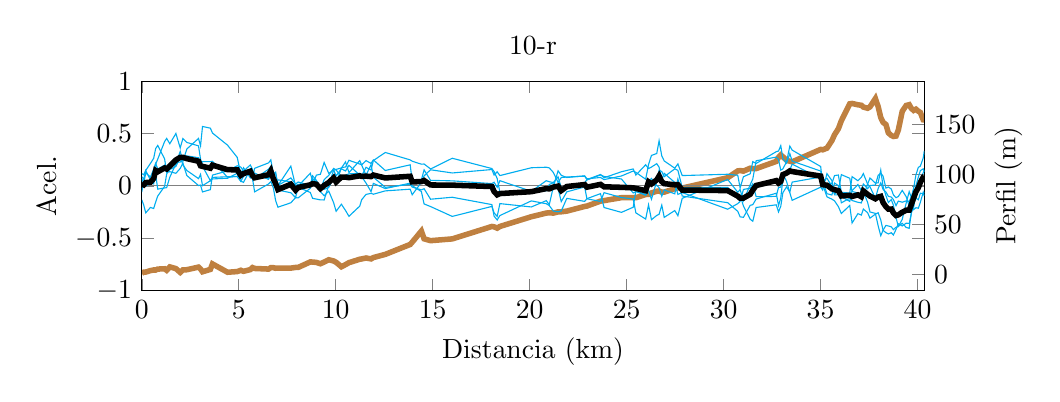
\begin{tikzpicture}
\pgfplotsset{width=0.95\textwidth, height=0.35\textwidth}
    \begin{axis}[
      axis y line*=right,
      axis x line=none,
      ylabel=Perfil (m),
      xmin=0,xmax=40346
    ]
    \addplot[color=brown, line width=2pt] coordinates {(0,0.87)(102.164,1.96)(203.92700000000002,2.08)(447.94500000000005,3.55)(613.325,4.17)(716.186,4.11)(823.47,5.07)(1176.592,5.38)(1282.9530000000002,3.84)(1445.4260000000002,7.25)(1759.0880000000002,5.55)(1982.15,1.73)(2119.9010000000003,4.26)(2322.943,4.41)(2924.277,7.04)(3030.437,5.18)(3130.813,2.38)(3536.143,4.74)(3644.949,10.22)(4420.9130000000005,1.9)(4921.3240000000005,2.56)(5104.733,3.87)(5245.344,2.82)(5594.861,4.54)(5710.807,6.57)(5817.772,5.68)(6534.901,5.07)(6654.088,6.53)(6783.7,6.45)(6902.016,5.91)(7020.003,5.97)(7685.297,6.03)(7928.504,6.71)(8062.249,6.71)(8688.872,12.23)(8807.58,12.11)(9002.436,11.74)(9210.017,10.43)(9403.583,12.11)(9641.305,14.38)(9892.713,13.19)(10020.635,11.84)(10293.636,7.4)(10506.469000000001,9.53)(10681.998000000001,11.49)(11237.900000000001,14.9)(11340.149000000001,15.22)(11563.322000000002,16.15)(11821.782000000003,15.26)(11939.827000000003,16.58)(12555.680000000002,19.79)(13839.171000000002,29.7)(13943.060000000001,31.97)(14416.667000000001,43.08)(14556.487000000001,35.35)(14890.702000000001,33.49)(16008.686000000002,35.26)(18050.462000000003,47.68)(18164.586000000003,47.34)(18325.663000000004,46.02)(18465.065000000002,47.71)(20084.003000000004,57.43)(20857.488000000005,61.1)(21009.720000000005,61.43)(21221.142000000003,61.07)(21465.656000000003,62.3)(21627.590000000004,62.37)(21915.516000000003,63.08)(22834.536000000004,67.72)(22952.991000000005,68.13)(23651.793000000005,73.07)(23836.670000000006,73.57)(24733.588000000007,76.53)(25338.191000000006,76.46)(25476.630000000005,76.46)(25981.370000000006,79.68)(26128.677000000007,79.76)(26280.104000000007,81.27)(26551.986000000008,82.92)(26672.823000000008,83.2)(26812.049000000006,82.04)(26937.280000000006,82.06)(27482.118000000006,85.47)(27643.210000000006,86.22)(27865.914000000008,86.13)(30208.929000000007,96.47)(30729.789000000008,103.29)(30851.175000000007,103.63)(31022.892000000007,103.08)(31373.032000000007,105.97)(31504.037000000008,105.6)(31676.333000000006,105.6)(32714.764000000006,112.78)(32831.530000000006,116.81)(32947.049000000006,119.15)(33057.22000000001,117.42)(33247.047000000006,113.82)(33414.321,113.0)(33535.26500000001,112.36)(35005.57600000001,124.81)(35109.21000000001,124.4)(35328.725000000006,126.05)(35584.062000000005,133.63)(35718.11400000001,139.43)(35917.28500000001,145.46)(36070.40500000001,153.45)(36503.86500000001,170.4)(36623.96900000001,170.76)(36926.16700000001,169.43)(37102.41000000001,168.93)(37205.05900000001,167.17)(37425.69800000001,165.97)(37546.65000000001,167.33)(37826.07800000001,175.65)(37968.48600000001,167.58)(38103.27700000001,156.65)(38220.99300000001,151.89)(38369.83800000001,149.67)(38495.22200000001,141.33)(38645.14800000001,138.8)(38754.81700000001,137.76)(38890.53500000001,138.18)(39007.28600000001,144.07)(39209.689000000006,162.84)(39413.97000000001,168.76)(39568.76400000001,169.54)(39678.03100000001,165.82)(39799.18100000001,163.8)(39916.84600000001,165.02)(40040.41400000001,163.02)(40144.534000000014,161.74)(40292.13800000001,154.38)(40345.99300000002,154.23)};
    \end{axis}
      \begin{axis}[
      title={10-r},
      xlabel={Distancia (km)},
      ylabel={Acel.},
      ymin=-1,ymax=1,xmin=0,xmax=40346,
      scaled x ticks = false,
      xtick={0,5000,10000,15000,20000,25000,30000,35000,40000},
      xticklabels={0,5,10,15,20,25,30,35,40}]
      
      \addplot[color=gray] coordinates {(0,0)(40346,0)};
      
      \addplot[color=cyan] coordinates {(0,-0.05764469)(102.164,0.03730226)(203.92700000000002,-0.00120893)(447.94500000000005,0.02547174)(613.325,0.12240078)(716.186,0.20749587)(823.47,0.25581752)(1176.592,0.4234229)(1282.9530000000002,0.4533229)(1445.4260000000002,0.40256507)(1759.0880000000002,0.50027095)(1982.15,0.3622442)(2119.9010000000003,0.452554)(2322.943,0.41505811)(2924.277,0.38229066)(3030.437,0.25560277)(3130.813,0.18824591)(3536.143,0.04956552)(3644.949,0.08139242)(4420.9130000000005,0.08770506)(4921.3240000000005,0.08844066)(5104.733,0.04363562)(5245.344,0.09100655)(5594.861,0.15541988)(5710.807,0.06657545)(5817.772,0.1680869)(6534.901,0.21973374)(6654.088,0.24903176)(6783.7,0.11767258)(6902.016,0.13196449)(7020.003,0.00394006)(7685.297,0.18893604)(7928.504,0.00208845)(8062.249,0.01536676)(8688.872,0.01109394)(8807.58,0.01467333)(9002.436,0.10300585)(9210.017,0.11130981)(9403.583,0.22376785)(9641.305,0.11902938)(9892.713,0.15242425)(10020.635,0.0955601)(10293.636,0.16379943)(10506.469000000001,0.14264271)(10681.998000000001,0.1964159)(11237.900000000001,0.1038768)(11340.149000000001,0.08773074)(11563.322000000002,0.02696751)(11821.782000000003,-0.05426614)(11939.827000000003,0.02403847)(12555.680000000002,-0.02511369)(13839.171000000002,0.02659241)(13943.060000000001,0.0030052)(14416.667000000001,-0.05378646)(14556.487000000001,-0.17193846)(14890.702000000001,-0.19674105)(16008.686000000002,-0.29092196)(18050.462000000003,-0.19534952)(18164.586000000003,-0.2562815)(18325.663000000004,-0.29103088)(18465.065000000002,-0.1685534)(20084.003000000004,-0.20074706)(20857.488000000005,-0.14039264)(21009.720000000005,-0.17936327)(21221.142000000003,-0.00855685)(21465.656000000003,0.14449486)(21627.590000000004,0.10111632)(21915.516000000003,0.08034903)(22834.536000000004,0.0965454)(22952.991000000005,0.06769488)(23651.793000000005,0.08082739)(23836.670000000006,0.06015124)(24733.588000000007,0.09504133)(25338.191000000006,0.14218155)(25476.630000000005,0.12930665)(25981.370000000006,0.06375874)(26128.677000000007,0.20377999)(26280.104000000007,0.29135768)(26551.986000000008,0.30898645)(26672.823000000008,0.43051018)(26812.049000000006,0.2860888)(26937.280000000006,0.23842108)(27482.118000000006,0.16951044)(27643.210000000006,0.21017808)(27865.914000000008,0.09887233)(30208.929000000007,0.11138115)(30729.789000000008,0.1014401)(30851.175000000007,-0.01836128)(31022.892000000007,0.08767817)(31373.032000000007,0.11616122)(31504.037000000008,0.23205562)(31676.333000000006,0.21407797)(32714.764000000006,0.32677315)(32831.530000000006,0.33299576)(32947.049000000006,0.38421818)(33057.22000000001,0.25977254)(33247.047000000006,0.2172085)(33414.321,0.30803212)(33535.26500000001,0.23674432)(35005.57600000001,0.14172024)(35109.21000000001,0.04657554)(35328.725000000006,0.07323096)(35584.062000000005,-0.00367815)(35718.11400000001,-0.07652509)(35917.28500000001,-0.05105387)(36070.40500000001,0.10778085)(36503.86500000001,0.07292706)(36623.96900000001,-0.05278348)(36926.16700000001,-0.06769338)(37102.41000000001,-0.11218867)(37205.05900000001,-0.05677243)(37425.69800000001,-0.15619897)(37546.65000000001,-0.24819328)(37826.07800000001,-0.26223791)(37968.48600000001,-0.38067917)(38103.27700000001,-0.47508609)(38220.99300000001,-0.42291495)(38369.83800000001,-0.37644343)(38495.22200000001,-0.3820591)(38645.14800000001,-0.39019571)(38754.81700000001,-0.41687663)(38890.53500000001,-0.39441749)(39007.28600000001,-0.38843151)(39209.689000000006,-0.31899586)(39413.97000000001,-0.16353829)(39568.76400000001,-0.05453248)(39678.03100000001,-0.10857511)(39799.18100000001,-0.02183622)(39916.84600000001,0.1060063)(40040.41400000001,0.17714055)(40144.534000000014,0.18924398)(40292.13800000001,0.26611807)(40345.99300000002,0.33303241)};

      \addplot[color=cyan] coordinates {(0,0.08881838)(102.164,0.06310958)(203.92700000000002,0.14561293)(447.94500000000005,0.0560338)(613.325,0.02153838)(716.186,0.10904543)(823.47,-0.03065186)(1176.592,-0.01936736)(1282.9530000000002,-0.01631189)(1445.4260000000002,0.08332335)(1759.0880000000002,0.21036737)(1982.15,0.329633)(2119.9010000000003,0.23436412)(2322.943,0.35241227)(2924.277,0.45293124)(3030.437,0.38245486)(3130.813,0.5672731)(3536.143,0.5510853)(3644.949,0.50479844)(4420.9130000000005,0.3890234)(4921.3240000000005,0.27261367)(5104.733,0.11379423)(5245.344,0.17335942)(5594.861,0.07667254)(5710.807,0.10957613)(5817.772,0.12271723)(6534.901,0.06228686)(6654.088,0.10513527)(6783.7,0.02106014)(6902.016,-0.02057263)(7020.003,-0.03919815)(7685.297,-0.06514428)(7928.504,-0.11099446)(8062.249,-0.0128113)(8688.872,-0.06223927)(8807.58,-0.11814913)(9002.436,-0.12529041)(9210.017,-0.13312988)(9403.583,-0.13380388)(9641.305,0.00820873)(9892.713,0.15029939)(10020.635,0.15802957)(10293.636,0.17100507)(10506.469000000001,0.22945588)(10681.998000000001,0.12723277)(11237.900000000001,0.24151949)(11340.149000000001,0.19743062)(11563.322000000002,0.10341591)(11821.782000000003,0.2028494)(11939.827000000003,0.08332632)(12555.680000000002,-0.01342922)(13839.171000000002,0.01514869)(13943.060000000001,-0.01081242)(14416.667000000001,-0.03793294)(14556.487000000001,-0.02674582)(14890.702000000001,-0.12689769)(16008.686000000002,-0.10808276)(18050.462000000003,-0.17800284)(18164.586000000003,-0.28770273)(18325.663000000004,-0.32483096)(18465.065000000002,-0.28272387)(20084.003000000004,-0.14275685)(20857.488000000005,-0.16989151)(21009.720000000005,-0.18674257)(21221.142000000003,-0.2396733)(21465.656000000003,-0.24650308)(21627.590000000004,-0.23937365)(21915.516000000003,-0.1186671)(22834.536000000004,-0.14733762)(22952.991000000005,-0.12150904)(23651.793000000005,-0.07363794)(23836.670000000006,-0.20607474)(24733.588000000007,-0.25224898)(25338.191000000006,-0.20343803)(25476.630000000005,-0.04082885)(25981.370000000006,-0.0871214)(26128.677000000007,-0.04418876)(26280.104000000007,-0.12675515)(26551.986000000008,0.04485331)(26672.823000000008,0.15023719)(26812.049000000006,0.13734182)(26937.280000000006,0.0879771)(27482.118000000006,0.16282395)(27643.210000000006,0.14819627)(27865.914000000008,-0.01556775)(30208.929000000007,-0.0140697)(30729.789000000008,-0.11750635)(30851.175000000007,-0.08794063)(31022.892000000007,-0.19279009)(31373.032000000007,-0.31818775)(31504.037000000008,-0.33677415)(31676.333000000006,-0.20578161)(32714.764000000006,-0.18015442)(32831.530000000006,-0.24791187)(32947.049000000006,-0.19450226)(33057.22000000001,-0.06367029)(33247.047000000006,-0.0087394)(33414.321,-0.05838407)(33535.26500000001,0.03650093)(35005.57600000001,0.08521273)(35109.21000000001,-0.00718094)(35328.725000000006,0.02181398)(35584.062000000005,0.02458001)(35718.11400000001,0.09884265)(35917.28500000001,0.1042193)(36070.40500000001,-0.06086127)(36503.86500000001,-0.06816587)(36623.96900000001,0.08860947)(36926.16700000001,0.04929726)(37102.41000000001,0.08223559)(37205.05900000001,0.11797357)(37425.69800000001,0.01704411)(37546.65000000001,-0.00831527)(37826.07800000001,-0.11704358)(37968.48600000001,-0.02434598)(38103.27700000001,0.0298401)(38220.99300000001,-0.03306373)(38369.83800000001,-0.05817551)(38495.22200000001,-0.0988534)(38645.14800000001,-0.10609427)(38754.81700000001,-0.13033161)(38890.53500000001,-0.18788645)(39007.28600000001,-0.14507504)(39209.689000000006,-0.15518327)(39413.97000000001,-0.1426646)(39568.76400000001,-0.14749168)(39678.03100000001,-0.10348788)(39799.18100000001,-0.22551667)(39916.84600000001,-0.20798394)(40040.41400000001,-0.21269733)(40144.534000000014,-0.15584483)(40292.13800000001,-0.06061285)(40345.99300000002,-0.09595991)};

      \addplot[color=cyan] coordinates {(0,0.06640323)(102.164,0.02549287)(203.92700000000002,0.12450614)(447.94500000000005,0.08463596)(613.325,0.16077283)(716.186,0.21637264)(823.47,0.16108505)(1176.592,0.19811305)(1282.9530000000002,0.12889599)(1445.4260000000002,0.15718107)(1759.0880000000002,0.18512519)(1982.15,0.27581934)(2119.9010000000003,0.20081498)(2322.943,0.14753357)(2924.277,0.06997267)(3030.437,0.11041883)(3130.813,0.00256298)(3536.143,0.04954889)(3644.949,0.06674501)(4420.9130000000005,0.07324858)(4921.3240000000005,0.12058418)(5104.733,0.04511507)(5245.344,0.03405884)(5594.861,0.15814348)(5710.807,0.06967307)(5817.772,-0.05651345)(6534.901,0.01852443)(6654.088,0.04148876)(6783.7,-0.01783968)(6902.016,-0.14006866)(7020.003,-0.20289324)(7685.297,-0.16081775)(7928.504,-0.1115629)(8062.249,-0.11418023)(8688.872,-0.02208349)(8807.58,0.07107718)(9002.436,0.03677525)(9210.017,-0.03561747)(9403.583,0.05993837)(9641.305,0.10108362)(9892.713,0.16718324)(10020.635,0.15195902)(10293.636,0.08828842)(10506.469000000001,0.10286878)(10681.998000000001,0.11533883)(11237.900000000001,0.12061608)(11340.149000000001,0.09802262)(11563.322000000002,0.17702538)(11821.782000000003,0.15229784)(11939.827000000003,0.24197446)(12555.680000000002,0.31909747)(13839.171000000002,0.2483768)(13943.060000000001,0.23595781)(14416.667000000001,0.20739384)(14556.487000000001,0.20926171)(14890.702000000001,0.16193165)(16008.686000000002,0.26401604)(18050.462000000003,0.16596478)(18164.586000000003,0.13707658)(18325.663000000004,0.07061405)(18465.065000000002,-0.06172456)(20084.003000000004,-0.05278139)(20857.488000000005,-0.04546375)(21009.720000000005,0.0130654)(21221.142000000003,0.03122753)(21465.656000000003,-0.02520268)(21627.590000000004,-0.14974336)(21915.516000000003,-0.05627646)(22834.536000000004,-0.01007252)(22952.991000000005,-0.12291878)(23651.793000000005,-0.14781293)(23836.670000000006,-0.06420699)(24733.588000000007,-0.11069852)(25338.191000000006,-0.12469809)(25476.630000000005,-0.25695717)(25981.370000000006,-0.31627423)(26128.677000000007,-0.18013556)(26280.104000000007,-0.32207818)(26551.986000000008,-0.28137286)(26672.823000000008,-0.27096687)(26812.049000000006,-0.18329635)(26937.280000000006,-0.30003322)(27482.118000000006,-0.23479053)(27643.210000000006,-0.28428335)(27865.914000000008,-0.11840896)(30208.929000000007,0.0615058)(30729.789000000008,-0.06010399)(30851.175000000007,-0.0348764)(31022.892000000007,-0.14166343)(31373.032000000007,0.01214275)(31504.037000000008,0.06556882)(31676.333000000006,0.24010969)(32714.764000000006,0.275056)(32831.530000000006,0.25182195)(32947.049000000006,0.15062517)(33057.22000000001,0.16280289)(33247.047000000006,0.23147186)(33414.321,0.38017386)(33535.26500000001,0.3415232)(35005.57600000001,0.18526964)(35109.21000000001,0.01309428)(35328.725000000006,-0.10362)(35584.062000000005,-0.12638897)(35718.11400000001,-0.1418517)(35917.28500000001,-0.19702459)(36070.40500000001,-0.26314519)(36503.86500000001,-0.18597455)(36623.96900000001,-0.35396438)(36926.16700000001,-0.26415721)(37102.41000000001,-0.27833258)(37205.05900000001,-0.22044497)(37425.69800000001,-0.25544703)(37546.65000000001,-0.30719603)(37826.07800000001,-0.26913002)(37968.48600000001,-0.25545659)(38103.27700000001,-0.32489482)(38220.99300000001,-0.42319226)(38369.83800000001,-0.44617601)(38495.22200000001,-0.45806398)(38645.14800000001,-0.44640061)(38754.81700000001,-0.46815945)(38890.53500000001,-0.41391551)(39007.28600000001,-0.36068151)(39209.689000000006,-0.38174119)(39413.97000000001,-0.35550559)(39568.76400000001,-0.35788461)(39678.03100000001,-0.26700298)(39799.18100000001,-0.08788609)(39916.84600000001,0.00196274)(40040.41400000001,0.08413709)(40144.534000000014,0.14618876)(40292.13800000001,0.16286277)(40345.99300000002,0.13701367)};

      \addplot[color=cyan] coordinates{(0,0.11758949)(102.164,0.10626176)(203.92700000000002,0.14816548)(447.94500000000005,0.2149336)(613.325,0.26341252)(716.186,0.35657955)(823.47,0.3859027)(1176.592,0.25847076)(1282.9530000000002,0.12915466)(1445.4260000000002,0.13613036)(1759.0880000000002,0.12043853)(1982.15,0.16693125)(2119.9010000000003,0.21749112)(2322.943,0.09907589)(2924.277,0.00382996)(3030.437,0.00799824)(3130.813,-0.0571953)(3536.143,-0.03557208)(3644.949,0.10348048)(4420.9130000000005,0.14316322)(4921.3240000000005,0.19231374)(5104.733,0.180004)(5245.344,0.14197396)(5594.861,0.19964355)(5710.807,0.15815182)(5817.772,0.06655681)(6534.901,0.15971382)(6654.088,0.18765298)(6783.7,0.11036243)(6902.016,0.01802564)(7020.003,0.05795076)(7685.297,0.03973422)(7928.504,0.00263439)(8062.249,-0.00189948)(8688.872,0.12112091)(8807.58,0.04698872)(9002.436,0.01325425)(9210.017,-0.0540171)(9403.583,-0.09374219)(9641.305,-0.04976668)(9892.713,-0.16064776)(10020.635,-0.24175486)(10293.636,-0.17454869)(10506.469000000001,-0.23498259)(10681.998000000001,-0.28952693)(11237.900000000001,-0.19279868)(11340.149000000001,-0.13074574)(11563.322000000002,-0.08100876)(11821.782000000003,-0.07050011)(11939.827000000003,-0.07916331)(12555.680000000002,-0.04721934)(13839.171000000002,-0.03106234)(13943.060000000001,-0.08415458)(14416.667000000001,0.0339366)(14556.487000000001,0.09620989)(14890.702000000001,0.15402468)(16008.686000000002,0.12373624)(18050.462000000003,0.15644609)(18164.586000000003,0.10464682)(18325.663000000004,0.13484846)(18465.065000000002,0.09874449)(20084.003000000004,0.17338638)(20857.488000000005,0.17845196)(21009.720000000005,0.17186458)(21221.142000000003,0.12867493)(21465.656000000003,0.03245997)(21627.590000000004,0.0800882)(21915.516000000003,0.08515584)(22834.536000000004,0.09310809)(22952.991000000005,0.06014281)(23651.793000000005,0.10901203)(23836.670000000006,0.07817642)(24733.588000000007,0.13539037)(25338.191000000006,0.16208536)(25476.630000000005,0.10357479)(25981.370000000006,0.20175275)(26128.677000000007,0.16618258)(26280.104000000007,0.18004719)(26551.986000000008,0.21257931)(26672.823000000008,0.1784665)(26812.049000000006,0.06247151)(26937.280000000006,0.12025434)(27482.118000000006,0.03321659)(27643.210000000006,-0.08062913)(27865.914000000008,-0.06343305)(30208.929000000007,-0.22215474)(30729.789000000008,-0.16918546)(30851.175000000007,-0.14777739)(31022.892000000007,-0.03342488)(31373.032000000007,-0.0220016)(31504.037000000008,0.02025687)(31676.333000000006,-0.1024107)(32714.764000000006,-0.09979354)(32831.530000000006,-0.01376369)(32947.049000000006,-0.01178284)(33057.22000000001,0.1148781)(33247.047000000006,0.0428842)(33414.321,-0.06630679)(33535.26500000001,-0.13712463)(35005.57600000001,-0.01187856)(35109.21000000001,-0.03959044)(35328.725000000006,0.11742882)(35584.062000000005,0.05060908)(35718.11400000001,-0.08576874)(35917.28500000001,-0.08446529)(36070.40500000001,-0.102115)(36503.86500000001,-0.14762959)(36623.96900000001,-0.04465409)(36926.16700000001,0.01311862)(37102.41000000001,-0.04463697)(37205.05900000001,0.01840095)(37425.69800000001,-0.02650413)(37546.65000000001,0.00336136)(37826.07800000001,0.00891759)(37968.48600000001,0.10112978)(38103.27700000001,0.12222355)(38220.99300000001,0.09394117)(38369.83800000001,-0.02124119)(38495.22200000001,-0.00987007)(38645.14800000001,-0.02931258)(38754.81700000001,-0.08521702)(38890.53500000001,-0.11233201)(39007.28600000001,-0.10153359)(39209.689000000006,-0.04256702)(39413.97000000001,-0.1021186)(39568.76400000001,-0.19314857)(39678.03100000001,-0.16179412)(39799.18100000001,-0.02874558)(39916.84600000001,-0.11643887)(40040.41400000001,-0.13173198)(40144.534000000014,-0.06961566)(40292.13800000001,-0.073225)(40345.99300000002,-0.05637576)};

      \addplot[color=cyan] coordinates {(0,-0.13272954)(102.164,-0.18363954)(203.92700000000002,-0.25689945)(447.94500000000005,-0.20487334)(613.325,-0.21549443)(716.186,-0.15314649)(823.47,-0.09613882)(1176.592,-0.00450867)(1282.9530000000002,0.11286238)(1445.4260000000002,0.1669049)(1759.0880000000002,0.22371928)(1982.15,0.22794047)(2119.9010000000003,0.25784888)(2322.943,0.28705626)(2924.277,0.26895139)(3030.437,0.20140895)(3130.813,0.23150836)(3536.143,0.23136702)(3644.949,0.23525022)(4420.9130000000005,0.08337977)(4921.3240000000005,0.09198656)(5104.733,0.1215778)(5245.344,0.14786661)(5594.861,0.10939543)(5710.807,0.09210731)(5817.772,0.08825681)(6534.901,0.07509082)(6654.088,0.13635604)(6783.7,0.1116381)(6902.016,0.12035367)(7020.003,0.00445009)(7685.297,0.0764043)(7928.504,0.01790455)(8062.249,0.03739083)(8688.872,0.00488934)(8807.58,0.09674009)(9002.436,0.05348023)(9210.017,-0.01664331)(9403.583,-0.03235628)(9641.305,-0.01390525)(9892.713,0.07638521)(10020.635,0.02339269)(10293.636,0.17425021)(10506.469000000001,0.18125522)(10681.998000000001,0.24460735)(11237.900000000001,0.2085389)(11340.149000000001,0.20192782)(11563.322000000002,0.2414762)(11821.782000000003,0.21467446)(11939.827000000003,0.24849633)(12555.680000000002,0.14733847)(13839.171000000002,0.2012775)(13943.060000000001,0.04772738)(14416.667000000001,0.05846097)(14556.487000000001,0.15298149)(14890.702000000001,0.0533182)(16008.686000000002,0.04841014)(18050.462000000003,0.02237556)(18164.586000000003,0.0353497)(18325.663000000004,-0.01310361)(18465.065000000002,0.04993115)(20084.003000000004,-0.05113952)(20857.488000000005,0.05005268)(21009.720000000005,0.03999807)(21221.142000000003,0.03250673)(21465.656000000003,0.08666895)(21627.590000000004,-0.01603341)(21915.516000000003,-0.01829991)(22834.536000000004,0.03285646)(22952.991000000005,0.05693862)(23651.793000000005,0.10470161)(23836.670000000006,0.09033234)(24733.588000000007,0.06589019)(25338.191000000006,-0.06695446)(25476.630000000005,-0.05436802)(25981.370000000006,-0.08704071)(26128.677000000007,0.04771859)(26280.104000000007,0.07096394)(26551.986000000008,0.00408061)(26672.823000000008,-0.01653999)(26812.049000000006,-0.097638)(26937.280000000006,-0.03738275)(27482.118000000006,-0.07562311)(27643.210000000006,0.06617357)(27865.914000000008,-0.09657249)(30208.929000000007,-0.15976884)(30729.789000000008,-0.2424078)(30851.175000000007,-0.29518517)(31022.892000000007,-0.29914654)(31373.032000000007,-0.18482272)(31504.037000000008,-0.17897114)(31676.333000000006,-0.12508819)(32714.764000000006,-0.06968369)(32831.530000000006,-0.18678995)(32947.049000000006,-0.11587153)(33057.22000000001,0.06774205)(33247.047000000006,0.12928211)(33414.321,0.15425703)(33535.26500000001,0.20788717)(35005.57600000001,0.06922213)(35109.21000000001,0.04538693)(35328.725000000006,-0.07416125)(35584.062000000005,-0.08662166)(35718.11400000001,0.02739503)(35917.28500000001,0.00255193)(36070.40500000001,-0.16124524)(36503.86500000001,-0.11714152)(36623.96900000001,-0.13882678)(36926.16700000001,-0.15622358)(37102.41000000001,-0.16205528)(37205.05900000001,-0.09932438)(37425.69800000001,0.01722551)(37546.65000000001,0.07537707)(37826.07800000001,0.0269759)(37968.48600000001,0.02996986)(38103.27700000001,0.15066569)(38220.99300000001,-0.00374497)(38369.83800000001,-0.0922888)(38495.22200000001,-0.15862866)(38645.14800000001,-0.13041652)(38754.81700000001,-0.18400599)(38890.53500000001,-0.30335301)(39007.28600000001,-0.38548879)(39209.689000000006,-0.35718826)(39413.97000000001,-0.39582189)(39568.76400000001,-0.40454526)(39678.03100000001,-0.2539097)(39799.18100000001,-0.20679902)(39916.84600000001,-0.06190363)(40040.41400000001,-0.00067556)(40144.534000000014,0.05735585)(40292.13800000001,0.12519977)(40345.99300000002,0.14598525)};
        
    \addplot[color=black, line width=2pt] coordinates {(0,0.016487376)(102.164,0.00970538600000001)(203.92700000000002,0.032035234)(447.94500000000005,0.035240352)(613.325,0.070526016)(716.186,0.1472694)(823.47,0.135202918)(1176.592,0.171226136)(1282.9530000000002,0.161584808)(1445.4260000000002,0.18922095)(1759.0880000000002,0.247984264)(1982.15,0.272513652)(2119.9010000000003,0.27261462)(2322.943,0.26022722)(2924.277,0.235595184)(3030.437,0.19157673)(3130.813,0.18647901)(3536.143,0.16919893)(3644.949,0.198333314)(4420.9130000000005,0.155304006)(4921.3240000000005,0.153187762)(5104.733,0.100825344)(5245.344,0.117653076)(5594.861,0.139854976)(5710.807,0.099216756)(5817.772,0.07782086)(6534.901,0.107069934)(6654.088,0.143932962)(6783.7,0.068578714)(6902.016,0.021940502)(7020.003,-0.035150096)(7685.297,0.015822506)(7928.504,-0.039985994)(8062.249,-0.015226684)(8688.872,0.010556286)(8807.58,0.022266038)(9002.436,0.016245034)(9210.017,-0.02561959)(9403.583,0.004760774)(9641.305,0.03292996)(9892.713,0.077128866)(10020.635,0.037437304)(10293.636,0.084558888)(10506.469000000001,0.084248)(10681.998000000001,0.078813584)(11237.900000000001,0.096350518)(11340.149000000001,0.090873212)(11563.322000000002,0.093575248)(11821.782000000003,0.08901109)(11939.827000000003,0.103734454)(12555.680000000002,0.076134738)(13839.171000000002,0.092066612)(13943.060000000001,0.038344678)(14416.667000000001,0.041614402)(14556.487000000001,0.051953762)(14890.702000000001,0.00912715799999999)(16008.686000000002,0.00743154)(18050.462000000003,-0.005713186)(18164.586000000003,-0.053382226)(18325.663000000004,-0.084700588)(18465.065000000002,-0.072865238)(20084.003000000004,-0.054807688)(20857.488000000005,-0.025448652)(21009.720000000005,-0.028235558)(21221.142000000003,-0.011164192)(21465.656000000003,-0.001616396)(21627.590000000004,-0.04478918)(21915.516000000003,-0.00554772)(22834.536000000004,0.013019962)(22952.991000000005,-0.011930302)(23651.793000000005,0.014618032)(23836.670000000006,-0.008324346)(24733.588000000007,-0.013325122)(25338.191000000006,-0.018164734)(25476.630000000005,-0.02385452)(25981.370000000006,-0.04498497)(26128.677000000007,0.038671368)(26280.104000000007,0.018707096)(26551.986000000008,0.057825364)(26672.823000000008,0.094341402)(26812.049000000006,0.040993556)(26937.280000000006,0.02184731)(27482.118000000006,0.011027468)(27643.210000000006,0.011927088)(27865.914000000008,-0.039021984)(30208.929000000007,-0.044621266)(30729.789000000008,-0.0975527)(30851.175000000007,-0.116828174)(31022.892000000007,-0.115869354)(31373.032000000007,-0.07934162)(31504.037000000008,-0.039572796)(31676.333000000006,0.004181432)(32714.764000000006,0.0504395)(32831.530000000006,0.02727044)(32947.049000000006,0.042537344)(33057.22000000001,0.108305058)(33247.047000000006,0.122421454)(33414.321,0.14355443)(33535.26500000001,0.137106198)(35005.57600000001,0.093909236)(35109.21000000001,0.011657074)(35328.725000000006,0.006938502)(35584.062000000005,-0.028299938)(35718.11400000001,-0.03558157)(35917.28500000001,-0.045154504)(36070.40500000001,-0.09591717)(36503.86500000001,-0.089196894)(36623.96900000001,-0.100323852)(36926.16700000001,-0.085131658)(37102.41000000001,-0.102995582)(37205.05900000001,-0.048033452)(37425.69800000001,-0.080776102)(37546.65000000001,-0.09699323)(37826.07800000001,-0.122503604)(37968.48600000001,-0.10587642)(38103.27700000001,-0.099450314)(38220.99300000001,-0.157794948)(38369.83800000001,-0.198864988)(38495.22200000001,-0.221495042)(38645.14800000001,-0.220483938)(38754.81700000001,-0.25691814)(38890.53500000001,-0.282380894)(39007.28600000001,-0.276242088)(39209.689000000006,-0.25113512)(39413.97000000001,-0.231929794)(39568.76400000001,-0.23152052)(39678.03100000001,-0.178953958)(39799.18100000001,-0.114156716)(39916.84600000001,-0.05567148)(40040.41400000001,-0.016765446)(40144.534000000014,0.03346562)(40292.13800000001,0.084068552)(40345.99300000002,0.092739132)};
      \end{axis}
       
\end{tikzpicture}
\end{subfigure}
\caption{Diferentes suavizados para la solución}
\label{fig:multi_avg_solution}
\end{figure}

Los resultados de estas pruebas se pueden ver en la figura \ref{fig:multi_avg_solution}, donde se utiliza una representación gráfica similar a la mencionada en el capítulo  \ref{results_visualization}, con la diferencia de que, en este caso, cada serie azul se corresponde a una ejecución del algoritmo genético (con su respectivo suavizado) y la línea negra se corresponde a la media de las diferentes ejecuciones.

Como hecho bastante apreciable, y esperado por la técnica utilizada, se puede ver cómo conforme se aumenta el número de elementos a considerar para el cálculo de la media móvil, la gráfica resultante tiende a dispersarse menos, lo cual puede conllevar problemas, ya que dicha solución suavizada deja de ser comparable con la propuesta del algoritmo genético. Para ello, se ha calculado, a partir de la solución suavizada, el consumo que estimaría el modelo para dicha solución.

A partir de dichos cálculos, se puede extraer la conclusión que, de media, el uso de 5 elementos subestima el consumo entorno a un 26\%, mientras que el uso de 10 elementos lo hace en un 15\%. Sin embargo, el uso de la media de 10 elementos provoca que, de forma aleatoria, el consumo estimado sea totalmente dispar entre las diferentes ejecuciones del algoritmo, siendo en algunos casos incluso superior, por lo que no se podría considerar como adecuado a la hora de ser utilizado, primando en todo caso el uso de 5 elementos y teniendo en cuenta la desviación más fija que puede tener sobre un resultado.

\newpage
\section{Pruebas con diferentes rutas}
A partir de todo lo expuesto anteriormente, se han realizado unas pruebas finales, cuya finalidad consiste en ver el efecto que tiene sobre los resultados que expone el modelo el tipo de ruta a realizar, es decir, cómo afecta el hecho de que la ruta pueda ser prácticamente plana, ascendente o descendente en general, o con subidas y bajadas notables durante la misma.

Para ello, se han analizado cuatro rutas diferentes. La primera de ellas, llamada ``Ruta A'' en esta sección, se trata de la misma ruta con la que se han ido realizando las pruebas anteriores, y que se correspondería con el ejemplo de una ruta con una ascensión continua durante la mayor parte del trayecto. En cuanto a la ``Ruta B'', esta se trata de una ruta prácticamente plana, con 10 metros de desnivel entre su punto más alto y más bajo. También se ha añadido una ``Ruta C'', en cuyo perfil se encuentran varias subidas y bajadas significativas, con varios cientos de metros de desnivel en las mismas. Finalmente, se ha definido una cuarta ruta, la ``Ruta D'', que se corresponde a la inversa de la ruta A, con la que se puede ver el efecto de una ruta con un perfil descendiente en su casi totalidad.

\begin{figure}[!htb]
% FIGURE 40
\begin{subfigure}[b]{\textwidth}
\centering
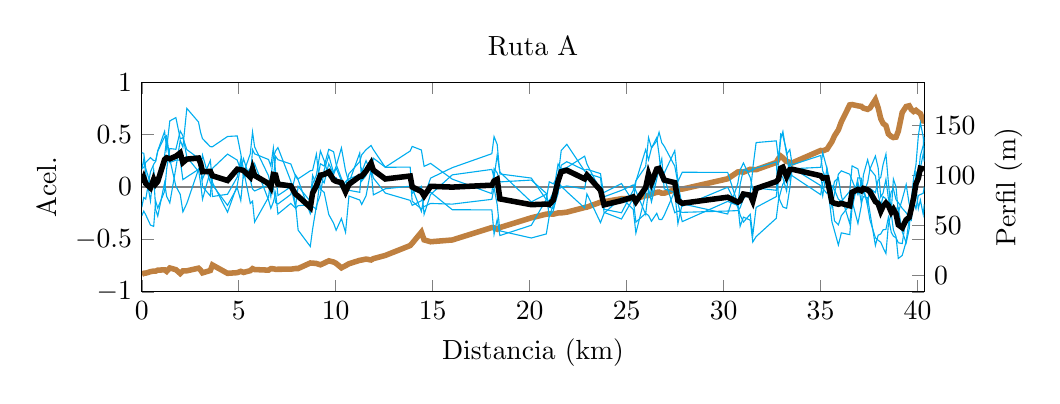
\begin{tikzpicture}
\pgfplotsset{%
    width=0.95\textwidth,
    height=0.35\textwidth
}
\begin{axis}[
      axis y line*=right,
      axis x line=none,
      ylabel=Perfil (m),
      xmin=0,xmax=40346
    ]
    \addplot[color=brown, line width=2pt] coordinates {(0,0.87)(102.164,1.96)(203.92700000000002,2.08)(447.94500000000005,3.55)(613.325,4.17)(716.186,4.11)(823.47,5.07)(1176.592,5.38)(1282.9530000000002,3.84)(1445.4260000000002,7.25)(1759.0880000000002,5.55)(1982.15,1.73)(2119.9010000000003,4.26)(2322.943,4.41)(2924.277,7.04)(3030.437,5.18)(3130.813,2.38)(3536.143,4.74)(3644.949,10.22)(4420.9130000000005,1.9)(4921.3240000000005,2.56)(5104.733,3.87)(5245.344,2.82)(5594.861,4.54)(5710.807,6.57)(5817.772,5.68)(6534.901,5.07)(6654.088,6.53)(6783.7,6.45)(6902.016,5.91)(7020.003,5.97)(7685.297,6.03)(7928.504,6.71)(8062.249,6.71)(8688.872,12.23)(8807.58,12.11)(9002.436,11.74)(9210.017,10.43)(9403.583,12.11)(9641.305,14.38)(9892.713,13.19)(10020.635,11.84)(10293.636,7.4)(10506.469000000001,9.53)(10681.998000000001,11.49)(11237.900000000001,14.9)(11340.149000000001,15.22)(11563.322000000002,16.15)(11821.782000000003,15.26)(11939.827000000003,16.58)(12555.680000000002,19.79)(13839.171000000002,29.7)(13943.060000000001,31.97)(14416.667000000001,43.08)(14556.487000000001,35.35)(14890.702000000001,33.49)(16008.686000000002,35.26)(18050.462000000003,47.68)(18164.586000000003,47.34)(18325.663000000004,46.02)(18465.065000000002,47.71)(20084.003000000004,57.43)(20857.488000000005,61.1)(21009.720000000005,61.43)(21221.142000000003,61.07)(21465.656000000003,62.3)(21627.590000000004,62.37)(21915.516000000003,63.08)(22834.536000000004,67.72)(22952.991000000005,68.13)(23651.793000000005,73.07)(23836.670000000006,73.57)(24733.588000000007,76.53)(25338.191000000006,76.46)(25476.630000000005,76.46)(25981.370000000006,79.68)(26128.677000000007,79.76)(26280.104000000007,81.27)(26551.986000000008,82.92)(26672.823000000008,83.2)(26812.049000000006,82.04)(26937.280000000006,82.06)(27482.118000000006,85.47)(27643.210000000006,86.22)(27865.914000000008,86.13)(30208.929000000007,96.47)(30729.789000000008,103.29)(30851.175000000007,103.63)(31022.892000000007,103.08)(31373.032000000007,105.97)(31504.037000000008,105.6)(31676.333000000006,105.6)(32714.764000000006,112.78)(32831.530000000006,116.81)(32947.049000000006,119.15)(33057.22000000001,117.42)(33247.047000000006,113.82)(33414.321,113.0)(33535.26500000001,112.36)(35005.57600000001,124.81)(35109.21000000001,124.4)(35328.725000000006,126.05)(35584.062000000005,133.63)(35718.11400000001,139.43)(35917.28500000001,145.46)(36070.40500000001,153.45)(36503.86500000001,170.4)(36623.96900000001,170.76)(36926.16700000001,169.43)(37102.41000000001,168.93)(37205.05900000001,167.17)(37425.69800000001,165.97)(37546.65000000001,167.33)(37826.07800000001,175.65)(37968.48600000001,167.58)(38103.27700000001,156.65)(38220.99300000001,151.89)(38369.83800000001,149.67)(38495.22200000001,141.33)(38645.14800000001,138.8)(38754.81700000001,137.76)(38890.53500000001,138.18)(39007.28600000001,144.07)(39209.689000000006,162.84)(39413.97000000001,168.76)(39568.76400000001,169.54)(39678.03100000001,165.82)(39799.18100000001,163.8)(39916.84600000001,165.02)(40040.41400000001,163.02)(40144.534000000014,161.74)(40292.13800000001,154.38)(40345.99300000002,154.23)};
    \end{axis}
      \begin{axis}[
      title={Ruta A},
      xlabel={Distancia (km)},
      ylabel={Acel.},
      ymin=-1,ymax=1,xmin=0,xmax=40346,
      scaled x ticks = false,
      xtick={0,5000,10000,15000,20000,25000,30000,35000,40000},
      xticklabels={0,5,10,15,20,25,30,35,40}]
      
      \addplot[color=gray] coordinates {(0,0)(40346,0)};
      
      \addplot[color=cyan] coordinates {(0,-0.1938196)(102.164,-0.10041567)(203.92700000000002,-0.11528936)(447.94500000000005,0.14409555)(613.325,0.21613233)(716.186,0.24476319)(823.47,0.34521723)(1176.592,0.5302811)(1282.9530000000002,0.3675395)(1445.4260000000002,0.63071348)(1759.0880000000002,0.66188262)(1982.15,0.45991292)(2119.9010000000003,0.47026081)(2322.943,0.35694891)(2924.277,0.27439452)(3030.437,0.16823361)(3130.813,0.3046684)(3536.143,0.04094474)(3644.949,0.01954292)(4420.9130000000005,-0.17526349)(4921.3240000000005,-0.00544876)(5104.733,-0.12925828)(5245.344,0.13593658)(5594.861,0.06772831)(5710.807,0.3572766)(5817.772,0.31628853)(6534.901,0.26240917)(6654.088,0.20023721)(6783.7,0.37173916)(6902.016,0.14078692)(7020.003,-0.08094336)(7685.297,0.0015198)(7928.504,-0.19235709)(8062.249,0.00613291)(8688.872,-0.13661002)(8807.58,0.11167688)(9002.436,0.02066809)(9210.017,0.22170375)(9403.583,0.19987879)(9641.305,0.35922964)(9892.713,0.33585882)(10020.635,0.21739068)(10293.636,0.08314475)(10506.469000000001,-0.00875858)(10681.998000000001,-0.03163079)(11237.900000000001,-0.0505734)(11340.149000000001,0.17544112)(11563.322000000002,0.12460884)(11821.782000000003,0.18422005)(11939.827000000003,0.0855658)(12555.680000000002,-0.05795887)(13839.171000000002,-0.12736418)(13943.060000000001,-0.17483622)(14416.667000000001,-0.13103523)(14556.487000000001,-0.07955541)(14890.702000000001,-0.04961404)(16008.686000000002,-0.21651274)(18050.462000000003,-0.21864587)(18164.586000000003,-0.45080869)(18325.663000000004,-0.31114363)(18465.065000000002,-0.46294896)(20084.003000000004,-0.36554901)(20857.488000000005,-0.11846092)(21009.720000000005,0.04931457)(21221.142000000003,0.03035835)(21465.656000000003,0.10422241)(21627.590000000004,0.34843531)(21915.516000000003,0.40745064)(22834.536000000004,0.15291808)(22952.991000000005,0.1303397)(23651.793000000005,0.08886839)(23836.670000000006,-0.21304556)(24733.588000000007,-0.24579585)(25338.191000000006,-0.03261559)(25476.630000000005,0.05974295)(25981.370000000006,0.1954947)(26128.677000000007,0.47165886)(26280.104000000007,0.37331334)(26551.986000000008,0.44017557)(26672.823000000008,0.52297241)(26812.049000000006,0.4224782)(26937.280000000006,0.38936149)(27482.118000000006,0.19886427)(27643.210000000006,0.0366666)(27865.914000000008,-0.18395153)(30208.929000000007,-0.00212205)(30729.789000000008,-0.19161683)(30851.175000000007,0.02389803)(31022.892000000007,0.1662136)(31373.032000000007,0.14722896)(31504.037000000008,0.17747839)(31676.333000000006,0.42393926)(32714.764000000006,0.44021322)(32831.530000000006,0.26194235)(32947.049000000006,0.50631733)(33057.22000000001,0.48851313)(33247.047000000006,0.34449711)(33414.321,0.07933187)(33535.26500000001,0.17247466)(35005.57600000001,0.10974691)(35109.21000000001,-0.0150245)(35328.725000000006,-0.06105663)(35584.062000000005,0.0138192)(35718.11400000001,-0.02601274)(35917.28500000001,-0.11710321)(36070.40500000001,-0.13802569)(36503.86500000001,-0.04105112)(36623.96900000001,0.20174249)(36926.16700000001,0.17186685)(37102.41000000001,0.01153626)(37205.05900000001,0.00263894)(37425.69800000001,-0.18332622)(37546.65000000001,-0.31528735)(37826.07800000001,-0.48426479)(37968.48600000001,-0.50792283)(38103.27700000001,-0.52711476)(38220.99300000001,-0.57803211)(38369.83800000001,-0.63488483)(38495.22200000001,-0.36156511)(38645.14800000001,-0.24496402)(38754.81700000001,-0.23700344)(38890.53500000001,-0.2023593)(39007.28600000001,-0.19886844)(39209.689000000006,-0.42726986)(39413.97000000001,-0.53189899)(39568.76400000001,-0.40098828)(39678.03100000001,-0.12471727)(39799.18100000001,0.08980349)(39916.84600000001,0.21011964)(40040.41400000001,0.48822656)(40144.534000000014,0.61300088)(40292.13800000001,0.47899837)(40345.99300000002,0.28868447)};

      \addplot[color=cyan] coordinates {(0,0.3274351)(102.164,0.32123635)(203.92700000000002,0.17763676)(447.94500000000005,0.02961158)(613.325,0.11287451)(716.186,-0.2153675)(823.47,-0.27815958)(1176.592,0.04045411)(1282.9530000000002,-0.09091531)(1445.4260000000002,-0.15160922)(1759.0880000000002,0.18274372)(1982.15,0.44480627)(2119.9010000000003,0.38028063)(2322.943,0.7501813)(2924.277,0.62033745)(3030.437,0.52208083)(3130.813,0.4610562)(3536.143,0.38462908)(3644.949,0.3843649)(4420.9130000000005,0.48183314)(4921.3240000000005,0.48751606)(5104.733,0.3169906)(5245.344,0.16059825)(5594.861,-0.15677643)(5710.807,-0.13511429)(5817.772,-0.33417098)(6534.901,-0.09783834)(6654.088,0.08483621)(6783.7,0.28135016)(6902.016,0.34538483)(7020.003,0.37629126)(7685.297,0.05669307)(7928.504,-0.1632325)(8062.249,-0.41163872)(8688.872,-0.56737376)(8807.58,-0.40191386)(9002.436,-0.18117162)(9210.017,-0.07306576)(9403.583,0.1610579)(9641.305,0.301114)(9892.713,0.13430611)(10020.635,0.19758907)(10293.636,0.37366453)(10506.469000000001,0.15500125)(10681.998000000001,0.04089614)(11237.900000000001,0.32460566)(11340.149000000001,0.05687647)(11563.322000000002,0.10937444)(11821.782000000003,0.23985999)(11939.827000000003,0.16593569)(12555.680000000002,0.08109315)(13839.171000000002,0.10977616)(13943.060000000001,-0.13623287)(14416.667000000001,-0.2095626)(14556.487000000001,-0.18756052)(14890.702000000001,-0.15695902)(16008.686000000002,-0.1632678)(18050.462000000003,-0.1175625)(18164.586000000003,-0.00660292)(18325.663000000004,-0.16844515)(18465.065000000002,-0.41844644)(20084.003000000004,-0.48639412)(20857.488000000005,-0.44788525)(21009.720000000005,-0.27891077)(21221.142000000003,-0.17133788)(21465.656000000003,0.04496131)(21627.590000000004,0.00704753)(21915.516000000003,-0.04512092)(22834.536000000004,-0.19983654)(22952.991000000005,-0.06599633)(23651.793000000005,-0.33963655)(23836.670000000006,-0.25006562)(24733.588000000007,-0.10215496)(25338.191000000006,-0.21231293)(25476.630000000005,-0.43850164)(25981.370000000006,-0.0672395)(26128.677000000007,0.16840792)(26280.104000000007,-0.07208785)(26551.986000000008,0.12393541)(26672.823000000008,0.18499133)(26812.049000000006,0.15694613)(26937.280000000006,0.13206646)(27482.118000000006,0.34677149)(27643.210000000006,0.0520188)(27865.914000000008,0.14065658)(30208.929000000007,0.13944641)(30729.789000000008,-0.16320197)(30851.175000000007,-0.3749109)(31022.892000000007,-0.2870315)(31373.032000000007,-0.31653783)(31504.037000000008,-0.52502658)(31676.333000000006,-0.47317354)(32714.764000000006,-0.2986374)(32831.530000000006,-0.12453173)(32947.049000000006,-0.04377102)(33057.22000000001,0.02920285)(33247.047000000006,0.08416903)(33414.321,0.17129681)(33535.26500000001,0.10705293)(35005.57600000001,-0.07299713)(35109.21000000001,0.04379901)(35328.725000000006,0.08625644)(35584.062000000005,-0.18565869)(35718.11400000001,-0.06342496)(35917.28500000001,0.12215716)(36070.40500000001,0.1538863)(36503.86500000001,0.12218216)(36623.96900000001,0.06393615)(36926.16700000001,-0.07290677)(37102.41000000001,0.05506178)(37205.05900000001,-0.05529179)(37425.69800000001,0.04228902)(37546.65000000001,0.17201098)(37826.07800000001,0.10699499)(37968.48600000001,-0.07169232)(38103.27700000001,-0.17879537)(38220.99300000001,-0.09098097)(38369.83800000001,-0.11233078)(38495.22200000001,-0.17312244)(38645.14800000001,-0.0446587)(38754.81700000001,-0.01891144)(38890.53500000001,-0.12120756)(39007.28600000001,-0.14833245)(39209.689000000006,-0.20265046)(39413.97000000001,-0.24549138)(39568.76400000001,-0.29145511)(39678.03100000001,-0.16412165)(39799.18100000001,-0.14665091)(39916.84600000001,-0.0043253)(40040.41400000001,-0.20554197)(40144.534000000014,-0.12451277)(40292.13800000001,-0.26127302)(40345.99300000002,-0.16503875)};

      \addplot[color=cyan] coordinates {(0,0.16728721)(102.164,0.2638998)(203.92700000000002,0.13280645)(447.94500000000005,-0.13377526)(613.325,0.16282272)(716.186,0.00198471)(823.47,0.05764586)(1176.592,0.29993883)(1282.9530000000002,0.45594536)(1445.4260000000002,0.23340337)(1759.0880000000002,0.25580728)(1982.15,0.25671627)(2119.9010000000003,0.07031154)(2322.943,0.09569332)(2924.277,0.1682266)(3030.437,0.03925987)(3130.813,-0.11677093)(3536.143,0.15052612)(3644.949,-0.09056735)(4420.9130000000005,-0.06912882)(4921.3240000000005,0.09423015)(5104.733,0.26326809)(5245.344,0.09064225)(5594.861,0.18079748)(5710.807,0.13724651)(5817.772,0.22205681)(6534.901,-0.12392194)(6654.088,-0.20366915)(6783.7,-0.14374862)(6902.016,-0.05426898)(7020.003,-0.25773617)(7685.297,-0.15621538)(7928.504,-0.20211733)(8062.249,-0.17788687)(8688.872,-0.16885682)(8807.58,0.02937571)(9002.436,0.1120484)(9210.017,0.34427169)(9403.583,0.25143738)(9641.305,0.09762189)(9892.713,0.09050103)(10020.635,0.09011883)(10293.636,-0.00990521)(10506.469000000001,0.05248067)(10681.998000000001,0.07895495)(11237.900000000001,0.11523653)(11340.149000000001,0.14055882)(11563.322000000002,0.25113738)(11821.782000000003,0.14356457)(11939.827000000003,0.27509581)(12555.680000000002,0.18935916)(13839.171000000002,0.34339011)(13943.060000000001,0.38705755)(14416.667000000001,0.35318903)(14556.487000000001,0.19681982)(14890.702000000001,0.22542853)(16008.686000000002,0.07513331)(18050.462000000003,-0.06319424)(18164.586000000003,0.17484304)(18325.663000000004,0.13510974)(18465.065000000002,0.04872463)(20084.003000000004,0.06609478)(20857.488000000005,-0.06025488)(21009.720000000005,-0.28040583)(21221.142000000003,-0.22603725)(21465.656000000003,-0.02259384)(21627.590000000004,-0.00363972)(21915.516000000003,0.00984952)(22834.536000000004,-0.01908089)(22952.991000000005,0.11348433)(23651.793000000005,0.00244879)(23836.670000000006,-0.24219785)(24733.588000000007,-0.30547538)(25338.191000000006,-0.10933309)(25476.630000000005,-0.33488136)(25981.370000000006,-0.25184497)(26128.677000000007,-0.27171649)(26280.104000000007,-0.32707309)(26551.986000000008,-0.25093804)(26672.823000000008,-0.30927499)(26812.049000000006,-0.31090074)(26937.280000000006,-0.27021724)(27482.118000000006,-0.03951961)(27643.210000000006,-0.34912841)(27865.914000000008,-0.16030608)(30208.929000000007,-0.25766596)(30729.789000000008,0.03339932)(30851.175000000007,0.16253122)(31022.892000000007,0.22892044)(31373.032000000007,0.09055327)(31504.037000000008,-0.02566089)(31676.333000000006,-0.00911382)(32714.764000000006,-0.03139357)(32831.530000000006,0.25129894)(32947.049000000006,0.45955873)(33057.22000000001,0.52930479)(33247.047000000006,0.31036415)(33414.321,0.35699936)(33535.26500000001,0.21164477)(35005.57600000001,0.30078899)(35109.21000000001,0.15374161)(35328.725000000006,0.06017514)(35584.062000000005,-0.3308108)(35718.11400000001,-0.41888478)(35917.28500000001,-0.55356692)(36070.40500000001,-0.43744501)(36503.86500000001,-0.45422432)(36623.96900000001,-0.19547958)(36926.16700000001,0.04693569)(37102.41000000001,-0.15436183)(37205.05900000001,-0.09086942)(37425.69800000001,-0.10244085)(37546.65000000001,-0.24541037)(37826.07800000001,-0.55782975)(37968.48600000001,-0.46003023)(38103.27700000001,-0.44739062)(38220.99300000001,-0.40847233)(38369.83800000001,-0.40437928)(38495.22200000001,-0.28855476)(38645.14800000001,-0.43232178)(38754.81700000001,-0.46873735)(38890.53500000001,-0.48432888)(39007.28600000001,-0.53193962)(39209.689000000006,-0.53927626)(39413.97000000001,-0.28904124)(39568.76400000001,-0.29474504)(39678.03100000001,-0.22668229)(39799.18100000001,-0.1838296)(39916.84600000001,0.0052703)(40040.41400000001,0.11326905)(40144.534000000014,0.29867052)(40292.13800000001,0.39495648)(40345.99300000002,0.47620711)};

      \addplot[color=cyan] coordinates{(0,0.17907696)(102.164,0.18520568)(203.92700000000002,0.23517898)(447.94500000000005,0.28091823)(613.325,0.25149063)(716.186,0.25079024)(823.47,0.34161935)(1176.592,0.47798012)(1282.9530000000002,0.49088717)(1445.4260000000002,0.26545089)(1759.0880000000002,0.00751908)(1982.15,-0.06935862)(2119.9010000000003,-0.23710306)(2322.943,-0.15702466)(2924.277,0.16953134)(3030.437,0.19063269)(3130.813,0.07701855)(3536.143,0.25309953)(3644.949,0.04263406)(4420.9130000000005,-0.2406755)(4921.3240000000005,0.01632826)(5104.733,0.20930789)(5245.344,0.13152794)(5594.861,0.31737393)(5710.807,0.52462341)(5817.772,0.38295885)(6534.901,0.10699575)(6654.088,0.00158569)(6783.7,0.00205371)(6902.016,-0.14931746)(7020.003,-0.162234)(7685.297,-0.07094448)(7928.504,0.11431584)(8062.249,0.07741472)(8688.872,0.15458624)(8807.58,0.15843503)(9002.436,0.31318629)(9210.017,-0.0203384)(9403.583,-0.05090623)(9641.305,-0.26262045)(9892.713,-0.34591941)(10020.635,-0.41271965)(10293.636,-0.30095712)(10506.469000000001,-0.43260348)(10681.998000000001,-0.08647692)(11237.900000000001,-0.12404577)(11340.149000000001,-0.16633421)(11563.322000000002,-0.08464023)(11821.782000000003,0.17111201)(11939.827000000003,-0.07554059)(12555.680000000002,-0.01695444)(13839.171000000002,0.00800759)(13943.060000000001,-0.00979845)(14416.667000000001,-0.23323669)(14556.487000000001,-0.09276857)(14890.702000000001,0.08482764)(16008.686000000002,0.1844122)(18050.462000000003,0.31784781)(18164.586000000003,0.48070917)(18325.663000000004,0.40566076)(18465.065000000002,0.124466)(20084.003000000004,0.08528471)(20857.488000000005,-0.12035882)(21009.720000000005,-0.1339364)(21221.142000000003,-0.04875685)(21465.656000000003,0.21926316)(21627.590000000004,0.17206515)(21915.516000000003,0.18527876)(22834.536000000004,0.29411281)(22952.991000000005,0.21906853)(23651.793000000005,-0.03304697)(23836.670000000006,-0.05177954)(24733.588000000007,0.0327453)(25338.191000000006,-0.13775997)(25476.630000000005,0.05171222)(25981.370000000006,0.35721768)(26128.677000000007,0.25892911)(26280.104000000007,0.37076021)(26551.986000000008,0.47012512)(26672.823000000008,0.30838216)(26812.049000000006,0.06794094)(26937.280000000006,0.0980039)(27482.118000000006,-0.24581719)(27643.210000000006,-0.22961645)(27865.914000000008,-0.24194898)(30208.929000000007,-0.2291992)(30729.789000000008,-0.22487)(30851.175000000007,-0.19849229)(31022.892000000007,-0.10875448)(31373.032000000007,-0.05360579)(31504.037000000008,0.16234944)(31676.333000000006,0.1808668)(32714.764000000006,0.23900603)(32831.530000000006,-0.09606692)(32947.049000000006,-0.14598129)(33057.22000000001,-0.18987682)(33247.047000000006,-0.20443248)(33414.321,-0.00924984)(33535.26500000001,0.18183532)(35005.57600000001,0.0133677)(35109.21000000001,-0.08437244)(35328.725000000006,0.18067535)(35584.062000000005,-0.06993104)(35718.11400000001,0.05302232)(35917.28500000001,0.08785045)(36070.40500000001,-0.08716504)(36503.86500000001,-0.34960594)(36623.96900000001,-0.13429895)(36926.16700000001,-0.3482815)(37102.41000000001,-0.17715862)(37205.05900000001,0.11340228)(37425.69800000001,0.26033199)(37546.65000000001,0.17110085)(37826.07800000001,0.29527323)(37968.48600000001,0.18388135)(38103.27700000001,-0.0955671)(38220.99300000001,-0.05807244)(38369.83800000001,0.07334625)(38495.22200000001,-0.1073909)(38645.14800000001,-0.22636373)(38754.81700000001,0.07582695)(38890.53500000001,-0.00055273)(39007.28600000001,-0.24378029)(39209.689000000006,-0.11727312)(39413.97000000001,0.02329656)(39568.76400000001,-0.16096099)(39678.03100000001,-0.20368447)(39799.18100000001,-0.14251686)(39916.84600000001,-0.20631512)(40040.41400000001,-0.08078772)(40144.534000000014,-0.07191675)(40292.13800000001,-0.05977948)(40345.99300000002,0.00328554)};

      \addplot[color=cyan] coordinates {(0,-0.27550861)(102.164,-0.23038073)(203.92700000000002,-0.26545908)(447.94500000000005,-0.36305246)(613.325,-0.37599255)(716.186,-0.13423807)(823.47,-0.20060813)(1176.592,-0.0408339)(1282.9530000000002,0.17077481)(1445.4260000000002,0.3669752)(1759.0880000000002,0.35996282)(1982.15,0.53441794)(2119.9010000000003,0.48827246)(2322.943,0.28510612)(2924.277,0.14872256)(3030.437,0.2141497)(3130.813,0.00348485)(3536.143,-0.08545456)(3644.949,0.17791059)(4420.9130000000005,0.31401147)(4921.3240000000005,0.25635073)(5104.733,0.16327469)(5245.344,0.26942768)(5594.861,0.06524501)(5710.807,-0.01827826)(5817.772,-0.03755988)(6534.901,0.02093994)(6654.088,-0.09291407)(6783.7,0.08493663)(6902.016,0.29099035)(7020.003,0.26083608)(7685.297,0.2197674)(7928.504,0.10181425)(8062.249,0.06787197)(8688.872,-0.25518124)(8807.58,-0.18605441)(9002.436,-0.20998872)(9210.017,0.09166593)(9403.583,0.03908849)(9641.305,0.22189462)(9892.713,0.12134185)(10020.635,0.18217822)(10293.636,0.06110449)(10506.469000000001,0.00769689)(10681.998000000001,0.12660579)(11237.900000000001,0.24116858)(11340.149000000001,0.30703648)(11563.322000000002,0.3559733)(11821.782000000003,0.39615875)(11939.827000000003,0.3563466)(12555.680000000002,0.18818035)(13839.171000000002,0.18995618)(13943.060000000001,-0.06129636)(14416.667000000001,0.00639626)(14556.487000000001,-0.26089184)(14890.702000000001,-0.0712584)(16008.686000000002,0.11600681)(18050.462000000003,0.16793276)(18164.586000000003,0.09042403)(18325.663000000004,0.30564296)(18465.065000000002,0.1419578)(20084.003000000004,-0.14221404)(20857.488000000005,-0.06807047)(21009.720000000005,-0.19270307)(21221.142000000003,-0.20553759)(21465.656000000003,-0.06196166)(21627.590000000004,0.2072275)(21915.516000000003,0.24140838)(22834.536000000004,0.16063626)(22952.991000000005,0.16893776)(23651.793000000005,0.12767459)(23836.670000000006,-0.09335027)(24733.588000000007,-0.03200515)(25338.191000000006,0.02002842)(25476.630000000005,-0.03715738)(25981.370000000006,-0.26158351)(26128.677000000007,-0.01538577)(26280.104000000007,-0.14207628)(26551.986000000008,0.07540876)(26672.823000000008,0.17908525)(26812.049000000006,0.26974473)(26937.280000000006,-0.01769421)(27482.118000000006,-0.05319973)(27643.210000000006,-0.15017427)(27865.914000000008,-0.33033148)(30208.929000000007,-0.13739759)(30729.789000000008,-0.17545076)(30851.175000000007,-0.26633795)(31022.892000000007,-0.33464133)(31373.032000000007,-0.26003885)(31504.037000000008,-0.46089549)(31676.333000000006,-0.19419468)(32714.764000000006,-0.09160432)(32831.530000000006,0.08446495)(32947.049000000006,0.12067146)(33057.22000000001,0.0873156)(33247.047000000006,-0.03754838)(33414.321,0.22708842)(33535.26500000001,0.17409927)(35005.57600000001,0.18784259)(35109.21000000001,0.32845874)(35328.725000000006,0.17599264)(35584.062000000005,-0.13631456)(35718.11400000001,-0.32242177)(35917.28500000001,-0.36108592)(36070.40500000001,-0.27366868)(36503.86500000001,-0.17088877)(36623.96900000001,-0.18617593)(36926.16700000001,0.08813873)(37102.41000000001,0.08343236)(37205.05900000001,-0.03877848)(37425.69800000001,-0.15322178)(37546.65000000001,-0.01247283)(37826.07800000001,-0.05368771)(37968.48600000001,0.06732178)(38103.27700000001,0.09273028)(38220.99300000001,0.21316151)(38369.83800000001,0.3138042)(38495.22200000001,0.04619778)(38645.14800000001,-0.25189937)(38754.81700000001,-0.4099876)(38890.53500000001,-0.47399455)(39007.28600000001,-0.68181617)(39209.689000000006,-0.6529038)(39413.97000000001,-0.51907822)(39568.76400000001,-0.30438892)(39678.03100000001,-0.31764923)(39799.18100000001,-0.12727434)(39916.84600000001,0.14508441)(40040.41400000001,0.10548017)(40144.534000000014,0.18058167)(40292.13800000001,0.31629811)(40345.99300000002,0.24198604)};
        
    \addplot[color=black, line width=2pt] coordinates {(0,0.040894192)(102.164,0.087909086)(203.92700000000002,0.03297475)(447.94500000000005,-0.00844047200000001)(613.325,0.073465528)(716.186,0.029586514)(823.47,0.053142946)(1176.592,0.261564052)(1282.9530000000002,0.278846306)(1445.4260000000002,0.268986744)(1759.0880000000002,0.293583104)(1982.15,0.325298956)(2119.9010000000003,0.234404476)(2322.943,0.266180998)(2924.277,0.276242494)(3030.437,0.22687134)(3130.813,0.145891414)(3536.143,0.148748982)(3644.949,0.106777024)(4420.9130000000005,0.06215536)(4921.3240000000005,0.169795288)(5104.733,0.164716598)(5245.344,0.15762654)(5594.861,0.09487366)(5710.807,0.173150794)(5817.772,0.109914666)(6534.901,0.033716916)(6654.088,-0.00198482199999999)(6783.7,0.119266208)(6902.016,0.114715132)(7020.003,0.027242762)(7685.297,0.010164082)(7928.504,-0.068315366)(8062.249,-0.087621198)(8688.872,-0.19468712)(8807.58,-0.05769613)(9002.436,0.010948488)(9210.017,0.112847442)(9403.583,0.120111266)(9641.305,0.14344794)(9892.713,0.06721768)(10020.635,0.05491143)(10293.636,0.041410288)(10506.469000000001,-0.04523665)(10681.998000000001,0.025669834)(11237.900000000001,0.10127832)(11340.149000000001,0.102715736)(11563.322000000002,0.151290746)(11821.782000000003,0.226983074)(11939.827000000003,0.161480662)(12555.680000000002,0.07674387)(13839.171000000002,0.104753172)(13943.060000000001,0.000978729999999996)(14416.667000000001,-0.042849846)(14556.487000000001,-0.084791304)(14890.702000000001,0.006484942)(16008.686000000002,-0.000845643999999998)(18050.462000000003,0.017275592)(18164.586000000003,0.057712926)(18325.663000000004,0.073364936)(18465.065000000002,-0.113249394)(20084.003000000004,-0.168555536)(20857.488000000005,-0.163006068)(21009.720000000005,-0.1673283)(21221.142000000003,-0.124262244)(21465.656000000003,0.056778276)(21627.590000000004,0.146227154)(21915.516000000003,0.159773276)(22834.536000000004,0.077749944)(22952.991000000005,0.113166798)(23651.793000000005,-0.03073835)(23836.670000000006,-0.170087768)(24733.588000000007,-0.130537208)(25338.191000000006,-0.094398632)(25476.630000000005,-0.139817042)(25981.370000000006,-0.00559112)(26128.677000000007,0.122378726)(26280.104000000007,0.040567266)(26551.986000000008,0.171741364)(26672.823000000008,0.177231232)(26812.049000000006,0.121241852)(26937.280000000006,0.06630408)(27482.118000000006,0.041419846)(27643.210000000006,-0.128046746)(27865.914000000008,-0.155176298)(30208.929000000007,-0.097387678)(30729.789000000008,-0.144348048)(30851.175000000007,-0.130662378)(31022.892000000007,-0.067058654)(31373.032000000007,-0.078480048)(31504.037000000008,-0.134351026)(31676.333000000006,-0.014335196)(32714.764000000006,0.051516792)(32831.530000000006,0.075421518)(32947.049000000006,0.179359042)(33057.22000000001,0.18889191)(33247.047000000006,0.099409886)(33414.321,0.165093324)(33535.26500000001,0.16942139)(35005.57600000001,0.107749812)(35109.21000000001,0.085320484)(35328.725000000006,0.088408588)(35584.062000000005,-0.141779178)(35718.11400000001,-0.155544386)(35917.28500000001,-0.164349688)(36070.40500000001,-0.156483624)(36503.86500000001,-0.178717598)(36623.96900000001,-0.050055164)(36926.16700000001,-0.0228494)(37102.41000000001,-0.03629801)(37205.05900000001,-0.013779694)(37425.69800000001,-0.027273568)(37546.65000000001,-0.046011744)(37826.07800000001,-0.138702806)(37968.48600000001,-0.15768845)(38103.27700000001,-0.231227514)(38220.99300000001,-0.184479268)(38369.83800000001,-0.152888888)(38495.22200000001,-0.176887086)(38645.14800000001,-0.24004152)(38754.81700000001,-0.211762576)(38890.53500000001,-0.256488604)(39007.28600000001,-0.360947394)(39209.689000000006,-0.3878747)(39413.97000000001,-0.312442654)(39568.76400000001,-0.290507668)(39678.03100000001,-0.207370982)(39799.18100000001,-0.102093644)(39916.84600000001,0.029966786)(40040.41400000001,0.084129218)(40144.534000000014,0.17916471)(40292.13800000001,0.173840092)(40345.99300000002,0.169024882)};
      \end{axis}
       
\end{tikzpicture}
\end{subfigure}
% FIGURE 41
\begin{subfigure}[b]{\textwidth}
\centering
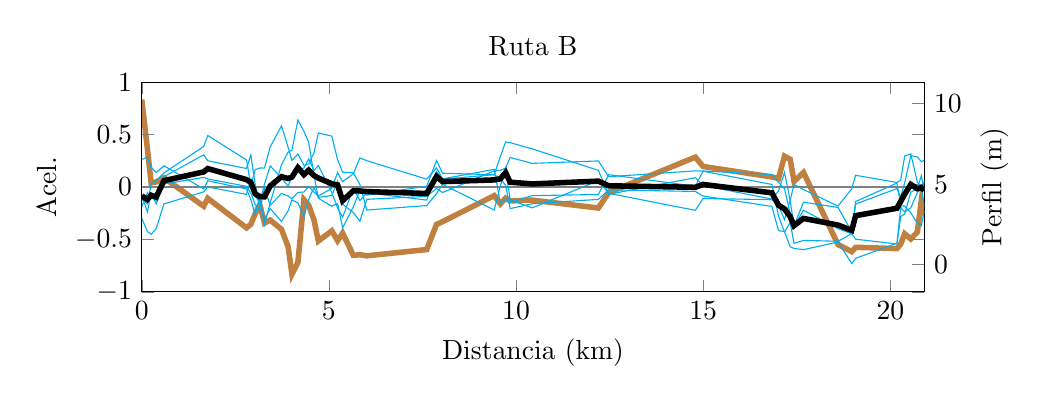
\begin{tikzpicture}
\pgfplotsset{width=0.95\textwidth, height=0.35\textwidth}
\begin{axis}[
      axis y line*=right,
      axis x line=none,
      ylabel=Perfil (m),
      xmin=0,xmax=20906
    ]
    \addplot[color=brown, line width=2pt] coordinates {(0,10.25)(150.065,7.19)(250.449,5.08)(385.27,5.14)(591.688,5.4)(1654.589,3.63)(1762.7949999999998,4.12)(2797.429,2.29)(2914.0080000000003,2.51)(3029.878,3.16)(3152.76,3.74)(3278.5280000000002,2.59)(3431.3460000000005,2.77)(3732.2900000000004,2.2)(3910.6540000000005,1.11)(4011.6850000000004,-0.6)(4171.204000000001,0.14)(4331.416000000001,4.04)(4458.840000000001,3.69)(4600.913000000001,2.78)(4718.266000000001,1.47)(5077.316000000002,2.1)(5231.606000000002,1.49)(5366.487000000002,1.96)(5653.278000000002,0.58)(5827.835000000002,0.62)(6012.496000000002,0.55)(7612.5340000000015,0.94)(7874.9450000000015,2.5)(8035.179000000002,2.67)(9416.470000000001,4.29)(9581.176000000001,3.78)(9720.686000000002,4.13)(9841.636000000002,3.96)(10429.308000000003,4.01)(12198.091000000002,3.52)(12475.574000000002,4.48)(14789.842000000002,6.68)(14996.804000000002,6.1)(16834.721,5.45)(17012.009000000002,5.35)(17171.573,6.74)(17324.215,6.54)(17425.969,5.17)(17679.566000000003,5.73)(18602.4,1.25)(18968.651,0.81)(19073.293,1.08)(20176.246000000003,1.0)(20276.381,1.28)(20382.744000000002,1.92)(20546.026,1.6)(20721.248000000003,2.03)(20827.932000000004,3.98)(20906.100000000006,3.07)};
    \end{axis}
      \begin{axis}[
      title={Ruta B},
      xlabel={Distancia (km)},
      ylabel={Acel.},
      ymin=-1,ymax=1,xmin=0,xmax=20906,
      scaled x ticks = false,
      xtick={0,5000,10000,15000,20000},
      xticklabels={0,5,10,15,20}]
      
      \addplot[color=gray] coordinates {(0,0)(20906,0)};
      
      \addplot[color=cyan] coordinates {(0,-0.18750584)(150.065,-0.05456519)(250.449,-0.10342107)(385.27,-0.12561305)(591.688,0.09827277)(1654.589,0.30651665)(1762.7949999999998,0.25064415)(2797.429,0.17646055)(2914.0080000000003,0.30660529)(3029.878,0.02176424)(3152.76,-0.15846754)(3278.5280000000002,-0.30739048)(3431.3460000000005,-0.20550014)(3732.2900000000004,-0.32908379)(3910.6540000000005,-0.22630099)(4011.6850000000004,-0.12248437)(4171.204000000001,-0.1514348)(4331.416000000001,-0.28219836)(4458.840000000001,-0.1184232)(4600.913000000001,-0.00429587)(4718.266000000001,-0.09934463)(5077.316000000002,-0.08059153)(5231.606000000002,0.05518678)(5366.487000000002,-0.16535157)(5653.278000000002,-0.24319127)(5827.835000000002,-0.32691589)(6012.496000000002,-0.11772997)(7612.5340000000015,-0.08910702)(7874.9450000000015,-0.01400062)(8035.179000000002,-0.05242101)(9416.470000000001,0.15393143)(9581.176000000001,0.15975152)(9720.686000000002,0.18059477)(9841.636000000002,0.28210035)(10429.308000000003,0.2254001)(12198.091000000002,0.24864697)(12475.574000000002,0.09843673)(14789.842000000002,0.1539498)(14996.804000000002,0.15281812)(16834.721,0.11902268)(17012.009000000002,0.04496487)(17171.573,-0.016546)(17324.215,-0.25228573)(17425.969,-0.37288538)(17679.566000000003,-0.22220942)(18602.4,-0.39702759)(18968.651,-0.44537423)(19073.293,-0.16222959)(20176.246000000003,-0.01505974)(20276.381,-0.09364541)(20382.744000000002,0.03921748)(20546.026,0.298793)(20721.248000000003,0.28619193)(20827.932000000004,0.24235215)(20906.100000000006,0.25548847)};

      \addplot[color=cyan] coordinates {(0,0.26305989)(150.065,0.28395427)(250.449,0.1877356)(385.27,0.13862098)(591.688,0.20237647)(1654.589,-0.01799272)(1762.7949999999998,0.05903493)(2797.429,-0.01799814)(2914.0080000000003,-0.11987954)(3029.878,-0.26259868)(3152.76,-0.10276767)(3278.5280000000002,-0.36063711)(3431.3460000000005,-0.15135884)(3732.2900000000004,0.21118649)(3910.6540000000005,0.33252501)(4011.6850000000004,0.35099462)(4171.204000000001,0.63903587)(4331.416000000001,0.53239811)(4458.840000000001,0.4259304)(4600.913000000001,0.11267334)(4718.266000000001,-0.10655735)(5077.316000000002,-0.18383618)(5231.606000000002,-0.15714625)(5366.487000000002,-0.39015981)(5653.278000000002,-0.1886544)(5827.835000000002,-0.03312982)(6012.496000000002,-0.07671881)(7612.5340000000015,0.00773926)(7874.9450000000015,0.25160757)(8035.179000000002,0.13136073)(9416.470000000001,0.11719266)(9581.176000000001,0.08276439)(9720.686000000002,0.01700155)(9841.636000000002,-0.20609776)(10429.308000000003,-0.15980114)(12198.091000000002,-0.11792214)(12475.574000000002,-0.02737068)(14789.842000000002,-0.04231875)(14996.804000000002,-0.08622386)(16834.721,-0.18497753)(17012.009000000002,-0.41625557)(17171.573,-0.42512633)(17324.215,-0.57089086)(17425.969,-0.58582076)(17679.566000000003,-0.59792269)(18602.4,-0.52413113)(18968.651,-0.73069966)(19073.293,-0.68029099)(20176.246000000003,-0.5359138)(20276.381,-0.19363466)(20382.744000000002,-0.23842918)(20546.026,-0.19897099)(20721.248000000003,-0.05430209)(20827.932000000004,-0.00742566)(20906.100000000006,-0.1936041)};

      \addplot[color=cyan] coordinates {(0,-0.120782626)(150.065,-0.159800412)(250.449,0.0285967455)(385.27,0.0610428874)(591.688,0.134417590)(1654.589,0.386264908)(1762.7949999999998,0.491843102)(2797.429,0.257996008)(2914.0080000000003,0.0164319922)(3029.878,0.166017316)(3152.76,0.181262435)(3278.5280000000002,0.180556357)(3431.3460000000005,0.382332066)(3732.2900000000004,0.583605647)(3910.6540000000005,0.378725917)(4011.6850000000004,0.253865767)(4171.204000000001,0.314782230)(4331.416000000001,0.206739548)(4458.840000000001,0.219664852)(4600.913000000001,0.326293727)(4718.266000000001,0.516147019)(5077.316000000002,0.484932959)(5231.606000000002,0.260663020)(5366.487000000002,0.141152181)(5653.278000000002,0.135474792)(5827.835000000002,0.0232642863)(6012.496000000002,-0.219769333)(7612.5340000000015,-0.176942073)(7874.9450000000015,-0.0639702937)(8035.179000000002,0.0255423962)(9416.470000000001,-0.219134707)(9581.176000000001,0.0127553162)(9720.686000000002,0.177222098)(9841.636000000002,-0.123233900)(10429.308000000003,-0.199324726)(12198.091000000002,0.0611659778)(12475.574000000002,-0.0604437420)(14789.842000000002,-0.222641262)(14996.804000000002,-0.109753411)(16834.721,-0.120800341)(17012.009000000002,-0.179480687)(17171.573,-0.312188622)(17324.215,-0.125724165)(17425.969,0.0240758506)(17679.566000000003,-0.0244085279)(18602.4,-0.182360160)(18968.651,-0.0170687424)(19073.293,0.111647594)(20176.246000000003,0.0436024107)(20276.381,0.0643456967)(20382.744000000002,0.294878334)(20546.026,0.316605254)(20721.248000000003,0.0467646764)(20827.932000000004,0.000104410612)(20906.100000000006,0.0488615424)};

      \addplot[color=cyan] coordinates{(0,-0.298979815)(150.065,-0.424705935)(250.449,-0.450860736)(385.27,-0.396349758)(591.688,-0.161639747)(1654.589,-0.0456853770)(1762.7949999999998,0.000337688204)(2797.429,-0.0702493306)(2914.0080000000003,0.0731391540)(3029.878,-0.0853275612)(3152.76,-0.151187336)(3278.5280000000002,0.0299568122)(3431.3460000000005,0.201234893)(3732.2900000000004,0.0864205517)(3910.6540000000005,0.00757133412)(4011.6850000000004,0.101962486)(4171.204000000001,0.172960224)(4331.416000000001,0.180144163)(4458.840000000001,0.267686036)(4600.913000000001,0.157655629)(4718.266000000001,0.205030758)(5077.316000000002,-0.0538342411)(5231.606000000002,-0.200325039)(5366.487000000002,-0.288172478)(5653.278000000002,-0.0114102407)(5827.835000000002,-0.129235336)(6012.496000000002,-0.0558441122)(7612.5340000000015,-0.124781367)(7874.9450000000015,0.145294158)(8035.179000000002,0.0750875726)(9416.470000000001,0.117654276)(9581.176000000001,0.290794425)(9720.686000000002,0.430319044)(9841.636000000002,0.423164226)(10429.308000000003,0.364077148)(12198.091000000002,0.159101003)(12475.574000000002,-0.0694855210)(14789.842000000002,0.0890527873)(14996.804000000002,0.0142953201)(16834.721,-0.115212194)(17012.009000000002,-0.0382772977)(17171.573,0.139066045)(17324.215,-0.130537166)(17425.969,-0.372284495)(17679.566000000003,-0.144456887)(18602.4,-0.195102748)(18968.651,-0.428618418)(19073.293,-0.137875617)(20176.246000000003,0.0371735585)(20276.381,-0.178919971)(20382.744000000002,-0.182086622)(20546.026,-0.245974413)(20721.248000000003,-0.347386869)(20827.932000000004,-0.368003662)(20906.100000000006,-0.227096375)};

      \addplot[color=cyan] coordinates {(0,-0.08214247)(150.065,-0.23777277)(250.449,-0.05635574)(385.27,-0.15926762)(591.688,0.0291736)(1654.589,0.09152972)(1762.7949999999998,0.07692456)(2797.429,0.00659549)(2914.0080000000003,-0.05567164)(3029.878,-0.16673974)(3152.76,-0.22534513)(3278.5280000000002,-0.01021422)(3431.3460000000005,-0.17398072)(3732.2900000000004,-0.06150111)(3910.6540000000005,-0.0861627)(4011.6850000000004,-0.11058745)(4171.204000000001,-0.05147144)(4331.416000000001,-0.04808375)(4458.840000000001,0.00465002)(4600.913000000001,-0.04902639)(4718.266000000001,-0.08651006)(5077.316000000002,-0.01282981)(5231.606000000002,0.1380599)(5366.487000000002,0.04978803)(5653.278000000002,0.12814493)(5827.835000000002,0.27777824)(6012.496000000002,0.25085876)(7612.5340000000015,0.0747489)(7874.9450000000015,0.18284424)(8035.179000000002,0.07742265)(9416.470000000001,0.16839551)(9581.176000000001,-0.15649379)(9720.686000000002,-0.11396802)(9841.636000000002,-0.14672499)(10429.308000000003,-0.08241672)(12198.091000000002,-0.07129082)(12475.574000000002,0.1173213)(14789.842000000002,0.00779884)(14996.804000000002,0.15075332)(16834.721,0.02443007)(17012.009000000002,-0.27632586)(17171.573,-0.43059052)(17324.215,-0.33779216)(17425.969,-0.5379586)(17679.566000000003,-0.50944191)(18602.4,-0.51766684)(18968.651,-0.44523635)(19073.293,-0.49775315)(20176.246000000003,-0.54366824)(20276.381,-0.28248503)(20382.744000000002,-0.25731239)(20546.026,-0.04939352)(20721.248000000003,-0.01339507)(20827.932000000004,0.10743678)(20906.100000000006,-0.04035117)};
        
    \addplot[color=black, line width=2pt] coordinates {(0,-0.0852701722)(150.065,-0.1185780074)(250.449,-0.0788610401)(385.27,-0.09631331212)(591.688,0.0605201366)(1654.589,0.1441266362)(1762.7949999999998,0.1757568860408)(2797.429,0.07056091548)(2914.0080000000003,0.04412505124)(3029.878,-0.06537688504)(3152.76,-0.0913010482)(3278.5280000000002,-0.09354572816)(3431.3460000000005,0.0105454518)(3732.2900000000004,0.09812555774)(3910.6540000000005,0.081271714224)(4011.6850000000004,0.0947502106)(4171.204000000001,0.1847744168)(4331.416000000001,0.1177999422)(4458.840000000001,0.1599016216)(4600.913000000001,0.1086600872)(4718.266000000001,0.0857531474)(5077.316000000002,0.03076823958)(5231.606000000002,0.0192876822)(5366.487000000002,-0.1305487294)(5653.278000000002,-0.03592723774)(5827.835000000002,-0.03764770394)(6012.496000000002,-0.04384069304)(7612.5340000000015,-0.06166846)(7874.9450000000015,0.10035501086)(8035.179000000002,0.05139846776)(9416.470000000001,0.0676078338)(9581.176000000001,0.07791437224)(9720.686000000002,0.1382338884)(9841.636000000002,0.0458415852)(10429.308000000003,0.0295869324)(12198.091000000002,0.05594019816)(12475.574000000002,0.0116916174)(14789.842000000002,-0.00283171694)(14996.804000000002,0.02437789782)(16834.721,-0.055507463)(17012.009000000002,-0.17307490894)(17171.573,-0.2090770854)(17324.215,-0.2834460162)(17425.969,-0.36897467688)(17679.566000000003,-0.29968788698)(18602.4,-0.3632576936)(18968.651,-0.41339948008)(19073.293,-0.2733003506)(20176.246000000003,-0.20277316216)(20276.381,-0.13686787486)(20382.744000000002,-0.0687464756)(20546.026,0.0242118662)(20721.248000000003,-0.01642548452)(20827.932000000004,-0.0051071962776)(20906.100000000006,-0.03134032652)};
      \end{axis}
       
\end{tikzpicture}
\end{subfigure}
% FIGURE 42
\begin{subfigure}[b]{\textwidth}
\centering
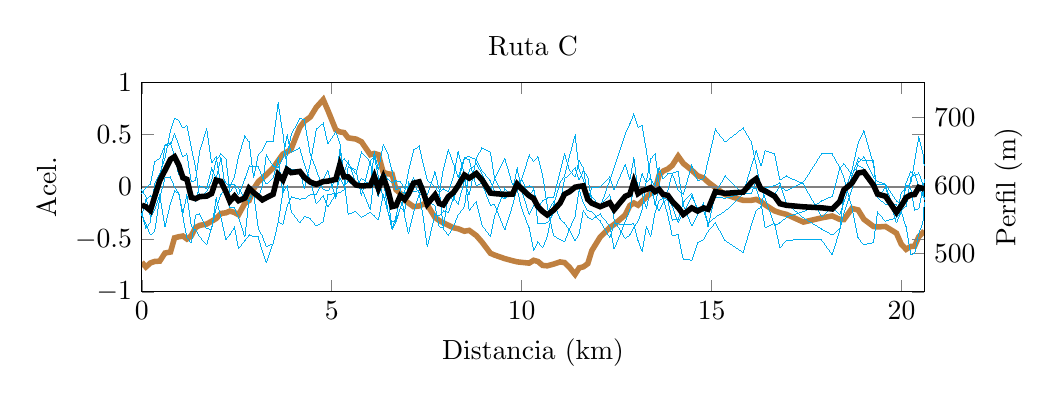
\begin{tikzpicture}
\pgfplotsset{width=0.95\textwidth, height=0.35\textwidth}
\begin{axis}[
      axis y line*=right,
      axis x line=none,
      ylabel=Perfil (m),
      xmin=0,xmax=20597
    ]
    \addplot[color=brown, line width=2pt] coordinates {(0,486.72)(108.472,479.77)(227.62099999999998,485.71)(338.258,487.91)(471.95899999999995,488.39)(611.2819999999999,500.32)(756.3309999999999,501.88)(861.728,522.72)(974.935,524.38)(1082.8609999999999,525.43)(1187.9709999999998,521.11)(1304.1419999999998,525.93)(1415.4009999999998,537.97)(1523.5829999999999,541.09)(1706.764,543.06)(1836.849,547.18)(1956.329,551.16)(2084.145,558.71)(2215.228,559.7)(2318.5660000000003,562.19)(2440.949,560.14)(2546.522,556.82)(2713.672,573.83)(2824.579,577.7)(2944.0150000000003,594.92)(3067.9980000000005,605.64)(3174.3420000000006,610.79)(3277.5900000000006,615.89)(3457.9060000000004,625.87)(3588.1630000000005,636.36)(3714.4510000000005,646.3)(3824.3520000000003,649.42)(3934.186,654.23)(4158.375,685.73)(4276.139,694.39)(4437.150000000001,701.05)(4593.89,715.32)(4776.068,726.58)(4897.731,710.94)(5106.63,682.06)(5212.193,679.04)(5325.755,677.96)(5432.854,670.21)(5637.347000000001,668.46)(5781.487000000001,664.49)(6015.442000000001,645.39)(6120.035000000001,647.26)(6227.8550000000005,645.37)(6355.274,619.43)(6478.035000000001,617.08)(6588.942000000001,616.62)(6690.840000000001,593.77)(6806.367000000001,588.26)(6920.366000000001,577.98)(7020.402000000001,574.09)(7154.499000000001,568.69)(7301.342000000001,569.76)(7409.217000000001,572.42)(7514.904,571.49)(7718.183000000001,552.82)(7829.549000000001,548.26)(7935.465000000001,544.89)(8068.313000000001,541.34)(8205.908000000001,537.63)(8325.502,536.24)(8493.390000000001,532.54)(8618.730000000001,533.78)(8804.831000000002,526.15)(8954.576000000003,516.59)(9177.170000000002,500.02)(9287.465000000002,497.32)(9555.906000000003,492.1)(9758.749000000003,489.02)(9878.933000000003,487.35)(9998.022000000003,486.61)(10197.023000000003,485.47)(10315.090000000004,489.62)(10428.969000000005,487.83)(10551.519000000004,482.12)(10673.188000000004,481.48)(10839.632000000003,484.03)(11009.262000000002,487.26)(11128.002000000002,486.3)(11256.971000000001,479.33)(11405.274000000001,468.91)(11512.400000000001,478.41)(11622.418000000001,479.95)(11740.240000000002,484.71)(11845.777000000002,503.85)(12065.261000000002,523.87)(12319.687000000002,538.1)(12434.572000000002,542.54)(12726.163000000002,556.54)(12848.116000000002,570.44)(12952.222000000002,574.14)(13062.579000000002,570.94)(13170.409000000001,577.03)(13283.754,582.57)(13397.85,588.73)(13511.002,592.79)(13615.665,614.98)(13723.284000000001,621.23)(13846.505000000001,624.29)(13964.111,629.62)(14119.054,643.15)(14254.755,632.54)(14476.973,622.47)(14631.661,614.29)(14789.317000000001,611.01)(14905.415,605.03)(15097.219000000001,596.89)(15354.891000000001,586.53)(15828.842,578.05)(16048.774000000001,578.17)(16172.980000000001,579.43)(16298.288000000002,576.2)(16409.091000000004,571.43)(16658.277000000006,562.42)(16797.274000000005,559.82)(16965.507000000005,557.44)(17416.634000000005,546.0)(17898.237000000005,552.25)(18173.344000000005,555.06)(18374.722000000005,549.93)(18480.998000000007,549.64)(18690.768000000007,566.1)(18856.32800000001,563.89)(19008.08100000001,550.13)(19259.519000000008,539.55)(19367.857000000007,538.79)(19577.440000000006,539.53)(19864.513000000006,529.61)(19989.632000000005,513.58)(20120.652000000006,505.84)(20242.690000000006,510.14)(20343.410000000007,510.5)(20452.121000000006,524.3)(20560.102000000006,530.45)(20597.272000000004,533.35)};
    \end{axis}
      \begin{axis}[
      title={Ruta C},
      xlabel={Distancia (km)},
      ylabel={Acel.},
      ymin=-1,ymax=1,xmin=0,xmax=20597,
      scaled x ticks = false,
      xtick={0,5000,10000,15000,20000},
      xticklabels={0,5,10,15,20}]
      
      \addplot[color=gray] coordinates {(0,0)(20597,0)};
      
      \addplot[color=cyan, line width=0mm] coordinates {(0,-0.0592756)(108.472,-0.00209388)(227.62099999999998,0.03013894)(338.258,0.24406457)(471.95899999999995,0.27626011)(611.2819999999999,0.40471666)(756.3309999999999,0.42314763)(861.728,0.3063519)(974.935,0.1163023)(1082.8609999999999,0.11091603)(1187.9709999999998,0.0152783)(1304.1419999999998,-0.02527476)(1415.4009999999998,-0.1352487)(1523.5829999999999,0.01465496)(1706.764,-0.01413758)(1836.849,0.18436295)(1956.329,0.07995688)(2084.145,0.28318593)(2215.228,-0.04205603)(2318.5660000000003,-0.19882849)(2440.949,-0.19777641)(2546.522,-0.28228657)(2713.672,-0.47593111)(2824.579,-0.10243104)(2944.0150000000003,-0.02735316)(3067.9980000000005,-0.09443589)(3174.3420000000006,0.01603319)(3277.5900000000006,0.30902626)(3457.9060000000004,0.20208396)(3588.1630000000005,0.18640405)(3714.4510000000005,0.27532485)(3824.3520000000003,0.49621537)(3934.186,0.33117993)(4158.375,0.37464895)(4276.139,0.22462758)(4437.150000000001,0.06208939)(4593.89,-0.15864559)(4776.068,-0.07853715)(4897.731,-0.18666301)(5106.63,-0.06610183)(5212.193,0.0912485)(5325.755,0.01207794)(5432.854,0.06151556)(5637.347000000001,-0.00460139)(5781.487000000001,0.08459348)(6015.442000000001,0.02384669)(6120.035000000001,0.34006247)(6227.8550000000005,0.16256996)(6355.274,0.41004203)(6478.035000000001,0.32063257)(6588.942000000001,0.15349775)(6690.840000000001,-0.0226184)(6806.367000000001,-0.01478718)(6920.366000000001,-0.27474609)(7020.402000000001,-0.44160355)(7154.499000000001,-0.235174)(7301.342000000001,-0.06185601)(7409.217000000001,-0.08181486)(7514.904,-0.07443295)(7718.183000000001,0.15212164)(7829.549000000001,-0.02272477)(7935.465000000001,-0.39027958)(8068.313000000001,-0.46035872)(8205.908000000001,-0.37092138)(8325.502,-0.26179251)(8493.390000000001,-0.18519632)(8618.730000000001,0.16558981)(8804.831000000002,0.22652446)(8954.576000000003,0.13063572)(9177.170000000002,-0.03813397)(9287.465000000002,0.08379238)(9555.906000000003,-0.09926534)(9758.749000000003,-0.06602573)(9878.933000000003,-0.00980341)(9998.022000000003,-0.02468498)(10197.023000000003,-0.26095517)(10315.090000000004,-0.17254339)(10428.969000000005,-0.17167366)(10551.519000000004,-0.23322132)(10673.188000000004,-0.2415703)(10839.632000000003,-0.13436786)(11009.262000000002,-0.3030856)(11128.002000000002,-0.33920814)(11256.971000000001,-0.40800405)(11405.274000000001,-0.51179058)(11512.400000000001,-0.44147648)(11622.418000000001,-0.22089678)(11740.240000000002,-0.28856242)(11845.777000000002,-0.30728454)(12065.261000000002,-0.25591019)(12319.687000000002,-0.36609511)(12434.572000000002,-0.59134211)(12726.163000000002,-0.32678215)(12848.116000000002,-0.2133637)(12952.222000000002,0.0126975)(13062.579000000002,-0.03017372)(13170.409000000001,-0.06730211)(13283.754,-0.20437184)(13397.85,-0.00475491)(13511.002,-0.14685138)(13615.665,-0.22439232)(13723.284000000001,-0.14065986)(13846.505000000001,-0.10534829)(13964.111,-0.17979804)(14119.054,-0.33734288)(14254.755,-0.24265366)(14476.973,-0.08366794)(14631.661,-0.19458531)(14789.317000000001,-0.21609447)(14905.415,-0.1745081)(15097.219000000001,-0.09897968)(15354.891000000001,-0.10640718)(15828.842,-0.05748931)(16048.774000000001,-0.00494632)(16172.980000000001,-0.01534858)(16298.288000000002,-0.14917601)(16409.091000000004,-0.38680902)(16658.277000000006,-0.34526149)(16797.274000000005,-0.57548899)(16965.507000000005,-0.50918337)(17416.634000000005,-0.49960516)(17898.237000000005,-0.50248595)(18173.344000000005,-0.64380467)(18374.722000000005,-0.40569786)(18480.998000000007,-0.25154343)(18690.768000000007,-0.0203561)(18856.32800000001,0.2400497)(19008.08100000001,0.29235873)(19259.519000000008,0.09589431)(19367.857000000007,0.05564293)(19577.440000000006,0.02768317)(19864.513000000006,-0.1286667)(19989.632000000005,-0.17077118)(20120.652000000006,0.01041687)(20242.690000000006,-0.01044362)(20343.410000000007,-0.21978129)(20452.121000000006,-0.20311296)(20560.102000000006,-0.01845653)(20597.272000000004,-0.11652781)};

      \addplot[color=cyan, line width=0mm] coordinates {(0,-0.25883339)(108.472,-0.34720288)(227.62099999999998,-0.45501755)(338.258,-0.42115932)(471.95899999999995,-0.10002834)(611.2819999999999,0.0899784)(756.3309999999999,0.09619286)(861.728,0.00740491)(974.935,-0.05928827)(1082.8609999999999,-0.27968643)(1187.9709999999998,-0.48015837)(1304.1419999999998,-0.53100084)(1415.4009999999998,-0.26820777)(1523.5829999999999,-0.25378547)(1706.764,-0.3952004)(1836.849,-0.40622069)(1956.329,-0.10460752)(2084.145,-0.28830309)(2215.228,-0.49735734)(2318.5660000000003,-0.45244847)(2440.949,-0.38075057)(2546.522,-0.58585308)(2713.672,-0.50799134)(2824.579,-0.45465232)(2944.0150000000003,-0.4737548)(3067.9980000000005,-0.47515272)(3174.3420000000006,-0.61244649)(3277.5900000000006,-0.71698049)(3457.9060000000004,-0.53129296)(3588.1630000000005,-0.33880951)(3714.4510000000005,-0.04559093)(3824.3520000000003,0.30162136)(3934.186,0.50751541)(4158.375,0.65466385)(4276.139,0.64631318)(4437.150000000001,0.3138294)(4593.89,0.1699282)(4776.068,-0.02118257)(4897.731,-0.03794728)(5106.63,0.07291124)(5212.193,0.3594625)(5325.755,0.14473668)(5432.854,0.25203579)(5637.347000000001,0.03454021)(5781.487000000001,-0.00692279)(6015.442000000001,-0.21187969)(6120.035000000001,0.12000239)(6227.8550000000005,0.06448091)(6355.274,0.15451884)(6478.035000000001,0.07683017)(6588.942000000001,0.04626741)(6690.840000000001,0.05836814)(6806.367000000001,0.0558817)(6920.366000000001,-0.01204807)(7020.402000000001,-0.00361575)(7154.499000000001,0.08683562)(7301.342000000001,-0.00620726)(7409.217000000001,-0.10727722)(7514.904,-0.12663968)(7718.183000000001,-0.1757305)(7829.549000000001,-0.3783202)(7935.465000000001,-0.39046414)(8068.313000000001,-0.07621056)(8205.908000000001,-0.12726555)(8325.502,0.04872809)(8493.390000000001,0.28016426)(8618.730000000001,0.29327119)(8804.831000000002,0.26195147)(8954.576000000003,0.16007769)(9177.170000000002,0.05970241)(9287.465000000002,-0.03870897)(9555.906000000003,-0.11340387)(9758.749000000003,-0.03038353)(9878.933000000003,0.18235984)(9998.022000000003,-0.02056823)(10197.023000000003,0.01256854)(10315.090000000004,-0.00645893)(10428.969000000005,-0.35106569)(10551.519000000004,-0.34669849)(10673.188000000004,-0.34210976)(10839.632000000003,-0.24517028)(11009.262000000002,-0.15967981)(11128.002000000002,0.08402353)(11256.971000000001,0.11879657)(11405.274000000001,0.18804786)(11512.400000000001,0.06724904)(11622.418000000001,0.16288476)(11740.240000000002,0.1007514)(11845.777000000002,-0.13911364)(12065.261000000002,-0.17451851)(12319.687000000002,-0.06946925)(12434.572000000002,-0.31273826)(12726.163000000002,-0.48775442)(12848.116000000002,-0.45682921)(12952.222000000002,-0.38230139)(13062.579000000002,-0.32216792)(13170.409000000001,-0.21386187)(13283.754,0.06748395)(13397.85,0.26960195)(13511.002,0.32124171)(13615.665,0.0449183)(13723.284000000001,-0.09748282)(13846.505000000001,-0.11983378)(13964.111,-0.31537377)(14119.054,-0.30947602)(14254.755,-0.14012919)(14476.973,-0.05835938)(14631.661,-0.21911207)(14789.317000000001,-0.22003803)(14905.415,-0.34320224)(15097.219000000001,-0.2867302)(15354.891000000001,-0.22740738)(15828.842,-0.06340393)(16048.774000000001,0.21039865)(16172.980000000001,0.34975812)(16298.288000000002,0.20143762)(16409.091000000004,0.34948226)(16658.277000000006,0.31576698)(16797.274000000005,0.0673502)(16965.507000000005,0.1063982)(17416.634000000005,0.02906021)(17898.237000000005,-0.28054385)(18173.344000000005,-0.18260752)(18374.722000000005,-0.25820723)(18480.998000000007,-0.14582763)(18690.768000000007,0.10598053)(18856.32800000001,0.27674615)(19008.08100000001,0.24977204)(19259.519000000008,0.24916365)(19367.857000000007,-0.09377252)(19577.440000000006,-0.16581328)(19864.513000000006,-0.16712279)(19989.632000000005,-0.2178405)(20120.652000000006,-0.18236228)(20242.690000000006,0.08770798)(20343.410000000007,0.13616429)(20452.121000000006,0.01055159)(20560.102000000006,-0.08495167)(20597.272000000004,0.06966238)};

      \addplot[color=cyan, line width=0mm] coordinates {(0,-0.25080308)(108.472,-0.39128854)(227.62099999999998,-0.32951193)(338.258,0.03818002)(471.95899999999995,0.13237727)(611.2819999999999,0.28488521)(756.3309999999999,0.54425031)(861.728,0.65710657)(974.935,0.63525045)(1082.8609999999999,0.56585302)(1187.9709999999998,0.58766797)(1304.1419999999998,0.38214675)(1415.4009999999998,0.18667861)(1523.5829999999999,-0.09528945)(1706.764,-0.03952774)(1836.849,0.06369628)(1956.329,0.25773875)(2084.145,0.31984419)(2215.228,0.27662304)(2318.5660000000003,-0.04891646)(2440.949,0.0164137)(2546.522,-0.0743418)(2713.672,0.08199853)(2824.579,0.20171852)(2944.0150000000003,0.19758247)(3067.9980000000005,0.19757203)(3174.3420000000006,0.09483589)(3277.5900000000006,0.02967201)(3457.9060000000004,0.08866707)(3588.1630000000005,0.27905189)(3714.4510000000005,-0.05212893)(3824.3520000000003,0.01679178)(3934.186,-0.22879694)(4158.375,-0.33995876)(4276.139,-0.2789664)(4437.150000000001,-0.29985786)(4593.89,-0.36849047)(4776.068,-0.3289724)(4897.731,-0.06883564)(5106.63,-0.06376617)(5212.193,-0.04927797)(5325.755,-0.02730042)(5432.854,0.19531377)(5637.347000000001,0.16806298)(5781.487000000001,-0.07869867)(6015.442000000001,0.25665124)(6120.035000000001,0.29529047)(6227.8550000000005,0.09698318)(6355.274,-0.10186761)(6478.035000000001,-0.07048312)(6588.942000000001,-0.40468774)(6690.840000000001,-0.32977117)(6806.367000000001,-0.1975827)(6920.366000000001,-0.04014343)(7020.402000000001,-0.09425644)(7154.499000000001,0.02320055)(7301.342000000001,-0.05033438)(7409.217000000001,-0.29143542)(7514.904,-0.57135802)(7718.183000000001,-0.25705809)(7829.549000000001,-0.27225413)(7935.465000000001,-0.227845)(8068.313000000001,-0.24032307)(8205.908000000001,-0.09401065)(8325.502,-0.16266228)(8493.390000000001,0.06702874)(8618.730000000001,-0.0762763)(8804.831000000002,0.2807944)(8954.576000000003,0.37449754)(9177.170000000002,0.3321245)(9287.465000000002,0.08444034)(9555.906000000003,0.27637821)(9758.749000000003,0.0268546)(9878.933000000003,-0.0164342)(9998.022000000003,0.07619257)(10197.023000000003,0.30620132)(10315.090000000004,0.24635067)(10428.969000000005,0.29383614)(10551.519000000004,0.1186049)(10673.188000000004,-0.17818967)(10839.632000000003,-0.46239404)(11009.262000000002,-0.49924788)(11128.002000000002,-0.51995822)(11256.971000000001,-0.39689761)(11405.274000000001,-0.27844428)(11512.400000000001,-0.01996623)(11622.418000000001,-0.15063906)(11740.240000000002,-0.22534072)(11845.777000000002,-0.23239545)(12065.261000000002,-0.32188728)(12319.687000000002,-0.47835868)(12434.572000000002,-0.34613461)(12726.163000000002,-0.360595)(12848.116000000002,-0.35655038)(12952.222000000002,-0.34812897)(13062.579000000002,-0.50840219)(13170.409000000001,-0.61311785)(13283.754,-0.37385644)(13397.85,-0.46943933)(13511.002,-0.23723671)(13615.665,-0.13225905)(13723.284000000001,-0.09659538)(13846.505000000001,-0.03154732)(13964.111,0.13359636)(14119.054,-0.02859883)(14254.755,-0.06765756)(14476.973,0.21209081)(14631.661,0.06104462)(14789.317000000001,0.07881941)(14905.415,0.2516062)(15097.219000000001,0.55354482)(15354.891000000001,0.43184784)(15828.842,0.56544734)(16048.774000000001,0.43289156)(16172.980000000001,0.21043095)(16298.288000000002,0.00727686)(16409.091000000004,-0.10602198)(16658.277000000006,-0.36387268)(16797.274000000005,-0.34295576)(16965.507000000005,-0.28413545)(17416.634000000005,-0.23371095)(17898.237000000005,-0.13324763)(18173.344000000005,-0.08584058)(18374.722000000005,0.18230107)(18480.998000000007,0.22705252)(18690.768000000007,0.12575671)(18856.32800000001,0.20808966)(19008.08100000001,0.18106063)(19259.519000000008,0.05488603)(19367.857000000007,0.02413197)(19577.440000000006,0.01987186)(19864.513000000006,-0.27961196)(19989.632000000005,-0.04949595)(20120.652000000006,0.00371933)(20242.690000000006,0.03971584)(20343.410000000007,0.25100382)(20452.121000000006,0.48113588)(20560.102000000006,0.32717738)(20597.272000000004,0.20119811)};

      \addplot[color=cyan, line width=0mm] coordinates{(0,-0.02791861)(108.472,-0.08587877)(227.62099999999998,-0.28528019)(338.258,-0.21449493)(471.95899999999995,-0.07077139)(611.2819999999999,-0.37604338)(756.3309999999999,-0.14977616)(861.728,-0.0375363)(974.935,-0.05581663)(1082.8609999999999,-0.24562504)(1187.9709999999998,-0.07509325)(1304.1419999999998,-0.37225051)(1415.4009999999998,-0.40667581)(1523.5829999999999,-0.46996473)(1706.764,-0.54882604)(1836.849,-0.38600204)(1956.329,-0.20220414)(2084.145,-0.067433)(2215.228,-0.01394981)(2318.5660000000003,0.01954897)(2440.949,0.02833126)(2546.522,-0.00418475)(2713.672,-0.11041167)(2824.579,-0.13482509)(2944.0150000000003,-0.0568191)(3067.9980000000005,-0.39167772)(3174.3420000000006,-0.46312391)(3277.5900000000006,-0.56681123)(3457.9060000000004,-0.54049723)(3588.1630000000005,-0.33124078)(3714.4510000000005,-0.35659705)(3824.3520000000003,-0.17871623)(3934.186,-0.09529185)(4158.375,-0.1146728)(4276.139,-0.11109855)(4437.150000000001,-0.06992709)(4593.89,-0.06989033)(4776.068,0.07675787)(4897.731,0.15853878)(5106.63,-0.10722304)(5212.193,0.2262712)(5325.755,0.27279217)(5432.854,0.22778914)(5637.347000000001,0.12881561)(5781.487000000001,0.33865916)(6015.442000000001,0.24261929)(6120.035000000001,0.03358733)(6227.8550000000005,-0.08830219)(6355.274,0.08234949)(6478.035000000001,-0.22690562)(6588.942000000001,-0.39891342)(6690.840000000001,-0.28245933)(6806.367000000001,-0.06907776)(6920.366000000001,-0.03624941)(7020.402000000001,0.15801292)(7154.499000000001,0.35444231)(7301.342000000001,0.3935955)(7409.217000000001,0.21893)(7514.904,0.07062963)(7718.183000000001,0.0048453)(7829.549000000001,-0.04594555)(7935.465000000001,-0.01522076)(8068.313000000001,-0.04589172)(8205.908000000001,0.1077516)(8325.502,0.33921116)(8493.390000000001,0.12471084)(8618.730000000001,-0.22001724)(8804.831000000002,-0.13411644)(8954.576000000003,-0.36018365)(9177.170000000002,-0.46891191)(9287.465000000002,-0.27692689)(9555.906000000003,-0.00898788)(9758.749000000003,-0.09470781)(9878.933000000003,-0.01836561)(9998.022000000003,-0.19749587)(10197.023000000003,-0.38932861)(10315.090000000004,-0.60340272)(10428.969000000005,-0.5178359)(10551.519000000004,-0.57916007)(10673.188000000004,-0.46759229)(10839.632000000003,-0.16631998)(11009.262000000002,0.04329209)(11128.002000000002,0.10845178)(11256.971000000001,0.29549706)(11405.274000000001,0.49666134)(11512.400000000001,0.16698343)(11622.418000000001,0.07587067)(11740.240000000002,-0.07423816)(11845.777000000002,-0.08385137)(12065.261000000002,-0.18825862)(12319.687000000002,0.06694181)(12434.572000000002,0.19293273)(12726.163000000002,0.51209553)(12848.116000000002,0.6076409)(12952.222000000002,0.70124574)(13062.579000000002,0.57199528)(13170.409000000001,0.5876893)(13283.754,0.34965321)(13397.85,0.07962324)(13511.002,0.01141319)(13615.665,0.18796562)(13723.284000000001,0.08114046)(13846.505000000001,0.12460002)(13964.111,0.13289482)(14119.054,0.14970993)(14254.755,-0.16751623)(14476.973,-0.36999691)(14631.661,-0.2630533)(14789.317000000001,-0.14562553)(14905.415,-0.37670739)(15097.219000000001,-0.05235286)(15354.891000000001,0.10842274)(15828.842,-0.06810047)(16048.774000000001,-0.05776425)(16172.980000000001,0.0657677)(16298.288000000002,0.03178892)(16409.091000000004,-0.03417601)(16658.277000000006,-0.06492807)(16797.274000000005,0.01317748)(16965.507000000005,-0.03575493)(17416.634000000005,0.05100091)(17898.237000000005,0.32285459)(18173.344000000005,0.31841603)(18374.722000000005,0.18879382)(18480.998000000007,0.09719955)(18690.768000000007,-0.1917483)(18856.32800000001,-0.48392608)(19008.08100000001,-0.54930294)(19259.519000000008,-0.53094288)(19367.857000000007,-0.23421493)(19577.440000000006,-0.3245239)(19864.513000000006,-0.29299212)(19989.632000000005,-0.23006811)(20120.652000000006,-0.38063665)(20242.690000000006,-0.64387153)(20343.410000000007,-0.62961694)(20452.121000000006,-0.44217317)(20560.102000000006,-0.33483012)(20597.272000000004,-0.1455076)};

      \addplot[color=cyan, line width=0mm] coordinates {(0,-0.26876662)(108.472,-0.1161532)(227.62099999999998,-0.08547591)(338.258,-0.10822744)(471.95899999999995,0.06562974)(611.2819999999999,0.39143533)(756.3309999999999,0.40705361)(861.728,0.51174796)(974.935,0.40475894)(1082.8609999999999,0.28871886)(1187.9709999999998,0.31712057)(1304.1419999999998,0.0499126)(1415.4009999999998,0.06625495)(1523.5829999999999,0.34387811)(1706.764,0.56181708)(1836.849,0.23220118)(1956.329,0.29385667)(2084.145,0.02172591)(2215.228,0.04795541)(2318.5660000000003,0.00213231)(2440.949,0.1025667)(2546.522,0.29477039)(2713.672,0.48857338)(2824.579,0.43112977)(2944.0150000000003,0.0915056)(3067.9980000000005,0.31483826)(3174.3420000000006,0.35036555)(3277.5900000000006,0.4346954)(3457.9060000000004,0.43599305)(3588.1630000000005,0.80193748)(3714.4510000000005,0.5140993)(3824.3520000000003,0.19210565)(3934.186,0.17061255)(4158.375,0.16889324)(4276.139,-0.01276968)(4437.150000000001,0.22781944)(4593.89,0.55590654)(4776.068,0.61068534)(4897.731,0.41403989)(5106.63,0.52700454)(5212.193,0.42776196)(5325.755,0.07689527)(5432.854,-0.25866109)(5637.347000000001,-0.22995851)(5781.487000000001,-0.28726972)(6015.442000000001,-0.23970649)(6120.035000000001,-0.27345535)(6227.8550000000005,-0.31116027)(6355.274,-0.06884215)(6478.035000000001,-0.23571773)(6588.942000000001,-0.33102692)(6690.840000000001,-0.31370881)(6806.367000000001,-0.19448572)(6920.366000000001,-0.23064205)(7020.402000000001,0.05429382)(7154.499000000001,-0.04483892)(7301.342000000001,-0.02935589)(7409.217000000001,0.01770385)(7514.904,-0.11340497)(7718.183000000001,-0.09770169)(7829.549000000001,-0.06625094)(7935.465000000001,0.17166503)(8068.313000000001,0.36080744)(8205.908000000001,0.2248242)(8325.502,0.09468605)(8493.390000000001,0.28450713)(8618.730000000001,0.25900314)(8804.831000000002,0.01202925)(8954.576000000003,0.03924329)(9177.170000000002,-0.17247963)(9287.465000000002,-0.16733682)(9555.906000000003,-0.40778958)(9758.749000000003,-0.17344234)(9878.933000000003,0.00499152)(9998.022000000003,0.08254565)(10197.023000000003,-0.08413467)(10315.090000000004,-0.01140665)(10428.969000000005,-0.19716477)(10551.519000000004,-0.12827211)(10673.188000000004,-0.10400419)(10839.632000000003,-0.09514691)(11009.262000000002,0.14807729)(11128.002000000002,0.32221488)(11256.971000000001,0.16589383)(11405.274000000001,0.0959117)(11512.400000000001,0.25528368)(11622.418000000001,0.18831698)(11740.240000000002,-0.10337879)(11845.777000000002,-0.00938329)(12065.261000000002,0.00181716)(12319.687000000002,0.09751662)(12434.572000000002,-0.02488934)(12726.163000000002,0.2184037)(12848.116000000002,0.07293553)(12952.222000000002,0.2797644)(13062.579000000002,-0.02312132)(13170.409000000001,0.13166318)(13283.754,0.04466017)(13397.85,0.0958971)(13511.002,-0.17218263)(13615.665,0.00757472)(13723.284000000001,-0.10187844)(13846.505000000001,-0.26539356)(13964.111,-0.46116863)(14119.054,-0.45415993)(14254.755,-0.69076734)(14476.973,-0.69704671)(14631.661,-0.53211924)(14789.317000000001,-0.4967708)(14905.415,-0.41918405)(15097.219000000001,-0.33735427)(15354.891000000001,-0.50902619)(15828.842,-0.62133705)(16048.774000000001,-0.35359177)(16172.980000000001,-0.22079706)(16298.288000000002,-0.19054086)(16409.091000000004,-0.00880863)(16658.277000000006,0.0152456)(16797.274000000005,0.04136463)(16965.507000000005,-0.14901576)(17416.634000000005,-0.29221912)(17898.237000000005,-0.39984412)(18173.344000000005,-0.45541241)(18374.722000000005,-0.39488586)(18480.998000000007,-0.06554595)(18690.768000000007,0.15870476)(18856.32800000001,0.42487587)(19008.08100000001,0.54240061)(19259.519000000008,0.22336243)(19367.857000000007,-0.09270484)(19577.440000000006,0.00118662)(19864.513000000006,-0.34174497)(19989.632000000005,-0.2297802)(20120.652000000006,0.04770737)(20242.690000000006,0.15163805)(20343.410000000007,0.10508975)(20452.121000000006,0.13632832)(20560.102000000006,0.03573852)(20597.272000000004,-0.11957236)};
        
    \addplot[color=black, line width=2pt] coordinates {(0,-0.17311946)(108.472,-0.188523454)(227.62099999999998,-0.225029328)(338.258,-0.09232742)(471.95899999999995,0.060693478)(611.2819999999999,0.158994444)(756.3309999999999,0.26417365)(861.728,0.289015008)(974.935,0.208241358)(1082.8609999999999,0.088035288)(1187.9709999999998,0.072963044)(1304.1419999999998,-0.099293352)(1415.4009999999998,-0.111439744)(1523.5829999999999,-0.092101316)(1706.764,-0.087174936)(1836.849,-0.062392464)(1956.329,0.064948128)(2084.145,0.053803988)(2215.228,-0.045756946)(2318.5660000000003,-0.135702428)(2440.949,-0.086243064)(2546.522,-0.130379162)(2713.672,-0.104752442)(2824.579,-0.011812032)(2944.0150000000003,-0.053767798)(3067.9980000000005,-0.089771208)(3174.3420000000006,-0.122867154)(3277.5900000000006,-0.10207961)(3457.9060000000004,-0.069009222)(3588.1630000000005,0.119468626)(3714.4510000000005,0.067021448)(3824.3520000000003,0.165603586)(3934.186,0.13704382)(4158.375,0.148714896)(4276.139,0.093621226)(4437.150000000001,0.046790656)(4593.89,0.02576167)(4776.068,0.051750218)(4897.731,0.055826548)(5106.63,0.072564948)(5212.193,0.211093238)(5325.755,0.095840328)(5432.854,0.095598634)(5637.347000000001,0.01937178)(5781.487000000001,0.010072292)(6015.442000000001,0.014306208)(6120.035000000001,0.103097462)(6227.8550000000005,-0.015085682)(6355.274,0.09524012)(6478.035000000001,-0.027128746)(6588.942000000001,-0.186972584)(6690.840000000001,-0.178037914)(6806.367000000001,-0.084010332)(6920.366000000001,-0.11876581)(7020.402000000001,-0.0654338)(7154.499000000001,0.036893112)(7301.342000000001,0.049168392)(7409.217000000001,-0.04877873)(7514.904,-0.163041198)(7718.183000000001,-0.074704668)(7829.549000000001,-0.157099118)(7935.465000000001,-0.17042889)(8068.313000000001,-0.092395326)(8205.908000000001,-0.051924356)(8325.502,0.011634102)(8493.390000000001,0.11424293)(8618.730000000001,0.08431412)(8804.831000000002,0.129436628)(8954.576000000003,0.068854118)(9177.170000000002,-0.05753972)(9287.465000000002,-0.062947992)(9555.906000000003,-0.070613692)(9758.749000000003,-0.067540962)(9878.933000000003,0.028549628)(9998.022000000003,-0.016802172)(10197.023000000003,-0.083129718)(10315.090000000004,-0.109492204)(10428.969000000005,-0.188780776)(10551.519000000004,-0.233749418)(10673.188000000004,-0.266693242)(10839.632000000003,-0.220679814)(11009.262000000002,-0.154128782)(11128.002000000002,-0.068895234)(11256.971000000001,-0.04494284)(11405.274000000001,-0.001922792)(11512.400000000001,0.00561468799999999)(11622.418000000001,0.011107314)(11740.240000000002,-0.118153738)(11845.777000000002,-0.154405658)(12065.261000000002,-0.187751488)(12319.687000000002,-0.149892922)(12434.572000000002,-0.216434318)(12726.163000000002,-0.088926468)(12848.116000000002,-0.069233372)(12952.222000000002,0.052655456)(13062.579000000002,-0.062373974)(13170.409000000001,-0.03498587)(13283.754,-0.02328619)(13397.85,-0.00581439)(13511.002,-0.044723164)(13615.665,-0.023238546)(13723.284000000001,-0.071095208)(13846.505000000001,-0.079504586)(13964.111,-0.137969852)(14119.054,-0.195973546)(14254.755,-0.261744796)(14476.973,-0.199396026)(14631.661,-0.22956506)(14789.317000000001,-0.199941884)(14905.415,-0.212399116)(15097.219000000001,-0.044374438)(15354.891000000001,-0.060514034)(15828.842,-0.048976684)(16048.774000000001,0.045397574)(16172.980000000001,0.077962226)(16298.288000000002,-0.019842694)(16409.091000000004,-0.037266676)(16658.277000000006,-0.088609932)(16797.274000000005,-0.159310488)(16965.507000000005,-0.174338262)(17416.634000000005,-0.189094822)(17898.237000000005,-0.198653392)(18173.344000000005,-0.20984983)(18374.722000000005,-0.137539212)(18480.998000000007,-0.027732988)(18690.768000000007,0.03566752)(18856.32800000001,0.13316706)(19008.08100000001,0.143257814)(19259.519000000008,0.018472708)(19367.857000000007,-0.068183478)(19577.440000000006,-0.088319106)(19864.513000000006,-0.242027708)(19989.632000000005,-0.179591188)(20120.652000000006,-0.100231072)(20242.690000000006,-0.075050656)(20343.410000000007,-0.071428074)(20452.121000000006,-0.003454068)(20560.102000000006,-0.015064484)(20597.272000000004,-0.022149456)};
      \end{axis}

\end{tikzpicture}
\end{subfigure}
% FIGURE 43
\begin{subfigure}[b]{\textwidth}
\centering
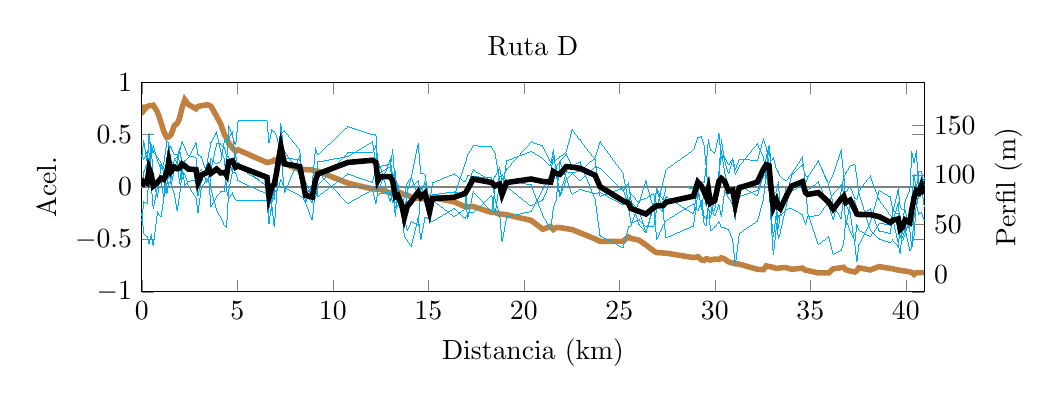
\begin{tikzpicture}
\pgfplotsset{width=0.95\textwidth, height=0.35\textwidth}
\begin{axis}[
      axis y line*=right,
      axis x line=none,
      ylabel=Perfil (m),
      xmin=0,xmax=40966
    ]
    \addplot[color=brown, line width=2pt] coordinates {(0,170.27)(100.372,164.72)(278.269,168.64)(382.569,169.44)(489.83000000000004,169.62)(601.6610000000001,170.12)(820.6880000000001,163.32)(1005.4430000000001,152.86)(1152.833,143.58)(1311.8960000000002,137.65)(1415.7420000000002,138.34)(1534.8220000000001,140.59)(1708.0620000000001,149.67)(1856.9070000000002,151.89)(1974.623,156.65)(2109.414,167.58)(2251.822,175.65)(2432.706,170.87)(2837.9610000000002,166.46)(2944.489,168.85)(3111.995,169.54)(3403.883,170.46)(3507.5449999999996,170.14)(3621.7389999999996,168.98)(3913.6949999999997,159.08)(4133.656,151.24)(4334.244,140.19)(4435.94,137.13)(4549.473,131.72)(4746.044,127.20)(4911.728,123.72)(5043.278,125.18)(6555.124,112.36)(6660.54,112.86)(6812.736,113.37)(6936.486,114.95)(7051.762,113.86)(7165.663,112.78)(7281.107,112.34)(7467.923,111.45)(8269.391,105.14)(8440.687,105.39)(8570.812,105.39)(8923.297,104.97)(9094.045,103.70)(9216.513,103.70)(10784.592,91.730)(12077.94,85.840)(12258.569000000001,85.760)(12359.838000000002,85.710)(12464.389000000001,85.700)(13007.535000000002,81.740)(13134.509000000002,82.870)(13277.310000000001,83.480)(13404.751000000002,83.390)(13613.420000000002,81.240)(13744.100000000002,80.130)(13900.193000000003,79.620)(14107.984000000002,77.600)(14471.996000000003,76.370)(14607.450000000003,76.370)(14824.332000000002,75.710)(15067.049000000003,77.350)(15211.207000000002,77.270)(16347.827000000001,72.890)(16933.68,67.970)(17063.144,67.720)(17352.027000000002,68.200)(18323.298000000003,62.180)(18491.471,62.190)(18735.191000000003,60.500)(18862.243000000002,60.560)(19099.535000000003,59.860)(20384.111000000004,54.240)(20995.867000000006,45.330)(21405.969000000005,48.160)(21544.635000000006,45.090)(21701.665000000005,47.110)(21885.576000000005,47.010)(22222.610000000004,45.870)(22527.314000000006,44.990)(22943.090000000007,41.730)(23734.243000000006,35.620)(23992.910000000007,33.160)(25192.392000000007,33.210)(25480.367000000006,37.630)(25598.906000000006,36.220)(26032.088000000007,34.290)(26394.840000000007,29.510)(26798.43800000001,23.620)(26958.72700000001,21.870)(27289.022000000008,21.430)(27445.356000000007,21.330)(28881.93600000001,16.830)(29113.00900000001,17.690)(29300.27300000001,14.460)(29438.894000000008,13.980)(29550.868000000006,15.660)(29659.059000000005,15.240)(29769.475000000006,14.320)(29998.109000000004,15.330)(30219.335000000003,14.920)(30339.831000000002,16.610)(30516.088000000003,15.330)(30721.116,12.530)(30938.123000000003,11.350)(31071.977000000003,10.670)(31278.726000000002,10.200)(32225.166,5.0800)(32544.376,4.7000)(32696.705,8.5200)(32837.449,7.6800)(32948.433,7.5700)(33064.717,6.9300)(33225.795,5.8900)(33326.595,6.2200)(33427.242,6.5100)(33722.186,6.8100)(34027.213,5.0500)(34584.207,6.2700)(34748.683000000005,3.8900)(34862.919,3.8500)(35418.575000000004,1.3500)(35958.688,1.3400)(36197.294,5.5300)(36610.631,6.6500)(36749.059,7.0300)(36856.223,4.5600)(37086.556,3.2700)(37335.14599999999,2.3600)(37439.581999999995,3.8100)(37540.952,6.5600)(38135.401,4.4100)(38606.229999999996,7.8000)(39192.356999999996,5.8800)(39320.142,5.4700)(39604.397,4.2500)(39706.502,4.1500)(39824.818,3.5700)(39964.906,3.3200)(40206.622,2.4600)(40314.594000000005,1.9200)(40432.100000000006,-0.040000)(40546.44300000001,1.5100)(40680.70300000001,1.6900)(40818.259000000005,1.7000)(40966.738000000005,1.5700)};
    \end{axis}
      \begin{axis}[
      title={Ruta D},
      xlabel={Distancia (km)},
      ylabel={Acel.},
      ymin=-1,ymax=1,xmin=0,xmax=40966,
      scaled x ticks = false,
      xtick={0,5000,10000,15000,20000,25000,30000,35000,40000},
      xticklabels={0,5,10,15,20,25,30,35,40}]
      
      \addplot[color=gray] coordinates {(0,0)(40966,0)};
      
      \addplot[color=cyan, line width=0mm] coordinates {(0,-0.24985196)(100.372,-0.43697951)(278.269,-0.47341029)(382.569,-0.54228141)(489.83000000000004,-0.45718295)(601.6610000000001,-0.55750575)(820.6880000000001,-0.23837335)(1005.4430000000001,-0.28582542)(1152.833,-0.10175351)(1311.8960000000002,0.02824823)(1415.7420000000002,0.12639577)(1534.8220000000001,0.08396786)(1708.0620000000001,0.27480782)(1856.9070000000002,0.23494538)(1974.623,0.33793756)(2109.414,0.43841106)(2251.822,0.37972027)(2432.706,0.30055809)(2837.9610000000002,0.28322405)(2944.489,-0.08063597)(3111.995,0.08070603)(3403.883,0.20125662)(3507.5449999999996,0.32838142)(3621.7389999999996,0.4232599)(3913.6949999999997,0.52502545)(4133.656,0.3410184)(4334.244,0.26711355)(4435.94,-0.02166206)(4549.473,-0.10300339)(4746.044,-0.05605609)(4911.728,-0.12104194)(5043.278,-0.12961846)(6555.124,-0.13122016)(6660.54,-0.34587038)(6812.736,-0.13418989)(6936.486,0.11061507)(7051.762,0.07427816)(7165.663,0.31908672)(7281.107,0.60336607)(7467.923,0.27878888)(8269.391,0.25847282)(8440.687,0.14810287)(8570.812,-0.06825943)(8923.297,-0.147136)(9094.045,0.10715342)(9216.513,-0.08938197)(10784.592,0.12514451)(12077.94,0.04552722)(12258.569000000001,0.20001944)(12359.838000000002,0.08070774)(12464.389000000001,0.13720798)(13007.535000000002,0.19661763)(13134.509000000002,0.35655324)(13277.310000000001,0.01729413)(13404.751000000002,-0.01756216)(13613.420000000002,-0.20144706)(13744.100000000002,-0.28619798)(13900.193000000003,-0.4139684)(14107.984000000002,-0.32558895)(14471.996000000003,-0.3628128)(14607.450000000003,-0.04523887)(14824.332000000002,-0.11765618)(15067.049000000003,-0.15176552)(15211.207000000002,0.03986695)(16347.827000000001,0.12591884)(16933.68,0.04849131)(17063.144,0.10921463)(17352.027000000002,0.09946073)(18323.298000000003,0.08818702)(18491.471,-0.11268567)(18735.191000000003,-0.25394209)(18862.243000000002,-0.52060114)(19099.535000000003,-0.28504857)(20384.111000000004,-0.2320682)(20995.867000000006,-0.01601645)(21405.969000000005,0.13549955)(21544.635000000006,0.28944126)(21701.665000000005,0.17097276)(21885.576000000005,-0.08749571)(22222.610000000004,0.07475372)(22527.314000000006,0.13342309)(22943.090000000007,0.15367633)(23734.243000000006,0.28269611)(23992.910000000007,0.43497621)(25192.392000000007,0.13762348)(25480.367000000006,-0.14710674)(25598.906000000006,-0.34326549)(26032.088000000007,-0.31133716)(26394.840000000007,-0.37410682)(26798.43800000001,-0.37517667)(26958.72700000001,-0.20013906)(27289.022000000008,0.05444535)(27445.356000000007,0.16860788)(28881.93600000001,0.35621677)(29113.00900000001,0.47168032)(29300.27300000001,0.48530522)(29438.894000000008,0.39874158)(29550.868000000006,0.18959644)(29659.059000000005,-0.0515049)(29769.475000000006,-0.17391478)(29998.109000000004,-0.27599431)(30219.335000000003,-0.16380642)(30339.831000000002,-0.2818164)(30516.088000000003,-0.03365479)(30721.116,-0.10157532)(30938.123000000003,-0.16671065)(31071.977000000003,-0.30526132)(31278.726000000002,0.02068873)(32225.166,-0.08110321)(32544.376,0.12167584)(32696.705,0.29519001)(32837.449,0.39959961)(32948.433,0.16157002)(33064.717,-0.06606546)(33225.795,-0.03800608)(33326.595,0.04938042)(33427.242,-0.18919809)(33722.186,-0.11935534)(34027.213,0.12146293)(34584.207,0.21389699)(34748.683000000005,0.11263807)(34862.919,0.09802017)(35418.575000000004,0.25256569)(35958.688,0.02496455)(36197.294,-0.16301743)(36610.631,-0.30189245)(36749.059,-0.09117343)(36856.223,-0.36333138)(37086.556,-0.16862474)(37335.14599999999,-0.13215818)(37439.581999999995,-0.19614769)(37540.952,-0.26947723)(38135.401,-0.20832815)(38606.229999999996,-0.41889304)(39192.356999999996,-0.44232523)(39320.142,-0.23122044)(39604.397,-0.01803651)(39706.502,-0.1800505)(39824.818,-0.21193529)(39964.906,-0.22101497)(40206.622,-0.4056935)(40314.594000000005,-0.57427006)(40432.100000000006,-0.45514644)(40546.44300000001,-0.16497431)(40680.70300000001,-0.08421688)(40818.259000000005,0.06561154)(40966.738000000005,0.0796266)};

      \addplot[color=cyan, line width=0mm] coordinates {(0,-0.3161989)(100.372,-0.1420659)(278.269,-0.15374134)(382.569,0.13545098)(489.83000000000004,0.32926186)(601.6610000000001,0.34353359)(820.6880000000001,0.2841238)(1005.4430000000001,0.23760605)(1152.833,0.13784399)(1311.8960000000002,0.01136841)(1415.7420000000002,0.23212696)(1534.8220000000001,0.02746787)(1708.0620000000001,0.17160548)(1856.9070000000002,0.25977297)(1974.623,0.36891924)(2109.414,0.23036694)(2251.822,0.22881002)(2432.706,0.20422891)(2837.9610000000002,0.16187345)(2944.489,0.09098133)(3111.995,0.03911844)(3403.883,0.21798284)(3507.5449999999996,0.21904579)(3621.7389999999996,-0.01728368)(3913.6949999999997,-0.21570956)(4133.656,-0.28710859)(4334.244,-0.3659757)(4435.94,-0.38597484)(4549.473,-0.03241567)(4746.044,0.15384434)(4911.728,0.31272387)(5043.278,0.19430898)(6555.124,0.01544896)(6660.54,-0.3162255)(6812.736,-0.18306745)(6936.486,-0.37925993)(7051.762,-0.10097418)(7165.663,0.22683657)(7281.107,0.33431972)(7467.923,-0.05347799)(8269.391,0.29740839)(8440.687,0.0517962)(8570.812,-0.15110251)(8923.297,0.03262673)(9094.045,0.3751627)(9216.513,0.30932093)(10784.592,0.57849559)(12077.94,0.49760587)(12258.569000000001,0.50125126)(12359.838000000002,0.18665134)(12464.389000000001,0.21210055)(13007.535000000002,-0.13715575)(13134.509000000002,-0.01264218)(13277.310000000001,-0.28391912)(13404.751000000002,0.03546851)(13613.420000000002,-0.21384037)(13744.100000000002,-0.08168717)(13900.193000000003,0.04617653)(14107.984000000002,0.09791966)(14471.996000000003,-0.07464185)(14607.450000000003,-0.00370616)(14824.332000000002,-0.06415784)(15067.049000000003,-0.33463466)(15211.207000000002,-0.32787141)(16347.827000000001,-0.20180047)(16933.68,-0.29755422)(17063.144,-0.24235569)(17352.027000000002,-0.24266773)(18323.298000000003,-0.07699339)(18491.471,-0.25653008)(18735.191000000003,0.04054637)(18862.243000000002,-0.03551939)(19099.535000000003,0.24930421)(20384.111000000004,0.34137672)(20995.867000000006,0.27514729)(21405.969000000005,0.20370737)(21544.635000000006,0.36111245)(21701.665000000005,0.12513419)(21885.576000000005,-0.08755422)(22222.610000000004,0.14888694)(22527.314000000006,0.13625322)(22943.090000000007,0.06499974)(23734.243000000006,0.19115703)(23992.910000000007,0.18063466)(25192.392000000007,-0.03629617)(25480.367000000006,0.04053149)(25598.906000000006,-0.10677985)(26032.088000000007,-0.35485466)(26394.840000000007,-0.43380022)(26798.43800000001,-0.16109145)(26958.72700000001,-0.50003557)(27289.022000000008,-0.35957606)(27445.356000000007,-0.31774513)(28881.93600000001,-0.15771343)(29113.00900000001,-0.22694662)(29300.27300000001,-0.12882923)(29438.894000000008,-0.27939666)(29550.868000000006,-0.30547402)(29659.059000000005,-0.17887636)(29769.475000000006,-0.28722768)(29998.109000000004,-0.09478578)(30219.335000000003,0.11225764)(30339.831000000002,0.35017361)(30516.088000000003,0.14218164)(30721.116,-0.02258282)(30938.123000000003,-0.02367504)(31071.977000000003,-0.08207565)(31278.726000000002,-0.09030318)(32225.166,-0.03093666)(32544.376,0.10056148)(32696.705,0.12857403)(32837.449,-0.03203278)(32948.433,-0.2687494)(33064.717,-0.47006456)(33225.795,-0.23613277)(33326.595,-0.4951666)(33427.242,-0.42969986)(33722.186,-0.19105877)(34027.213,0.03793722)(34584.207,-0.0101882)(34748.683000000005,-0.07340372)(34862.919,-0.02841785)(35418.575000000004,0.05009917)(35958.688,-0.16915887)(36197.294,-0.31029295)(36610.631,-0.03950235)(36749.059,0.09571036)(36856.223,0.13504095)(37086.556,0.20351393)(37335.14599999999,0.21935704)(37439.581999999995,0.09493447)(37540.952,-0.0507382)(38135.401,-0.40602297)(38606.229999999996,-0.49527582)(39192.356999999996,-0.5289136)(39320.142,-0.5055798)(39604.397,-0.56765715)(39706.502,-0.35584497)(39824.818,-0.3216748)(39964.906,-0.38196999)(40206.622,-0.39062592)(40314.594000000005,-0.16484787)(40432.100000000006,-0.16072871)(40546.44300000001,-0.15488818)(40680.70300000001,-0.25882775)(40818.259000000005,-0.24035011)(40966.738000000005,-0.31432763)};

      \addplot[color=cyan, line width=0mm] coordinates {(0,0.28664006)(100.372,0.43936407)(278.269,0.24307472)(382.569,0.44607113)(489.83000000000004,0.41016033)(601.6610000000001,0.07364398)(820.6880000000001,-0.10040601)(1005.4430000000001,0.21500014)(1152.833,0.19428636)(1311.8960000000002,-0.05987786)(1415.7420000000002,0.03892621)(1534.8220000000001,0.04051746)(1708.0620000000001,-0.06924755)(1856.9070000000002,-0.22551876)(1974.623,-0.08252705)(2109.414,0.12954093)(2251.822,0.25480576)(2432.706,0.28029661)(2837.9610000000002,0.42357067)(2944.489,0.31152637)(3111.995,0.29081455)(3403.883,0.13597605)(3507.5449999999996,0.17702299)(3621.7389999999996,0.16734638)(3913.6949999999997,0.41065952)(4133.656,0.41261074)(4334.244,0.37559168)(4435.94,0.29633963)(4549.473,0.29215405)(4746.044,0.13556836)(4911.728,0.14312581)(5043.278,0.0615067)(6555.124,-0.06499234)(6660.54,-0.1973392)(6812.736,-0.07195111)(6936.486,-0.11461166)(7051.762,0.25012202)(7165.663,0.37398918)(7281.107,0.50980087)(7467.923,0.53990385)(8269.391,0.35853514)(8440.687,0.00255431)(8570.812,0.05512459)(8923.297,-0.0793602)(9094.045,-0.11402879)(9216.513,0.01756824)(10784.592,0.33135748)(12077.94,0.32480481)(12258.569000000001,0.39473889)(12359.838000000002,0.16512777)(12464.389000000001,0.19829635)(13007.535000000002,0.21715027)(13134.509000000002,-0.01207219)(13277.310000000001,-0.1992285)(13404.751000000002,-0.17818124)(13613.420000000002,-0.11723188)(13744.100000000002,-0.36081049)(13900.193000000003,-0.00518871)(14107.984000000002,0.00536991)(14471.996000000003,0.06022646)(14607.450000000003,-0.06983395)(14824.332000000002,0.04932942)(15067.049000000003,-0.22556516)(15211.207000000002,-0.0742825)(16347.827000000001,-0.04676444)(16933.68,-0.07247258)(17063.144,-0.29771133)(17352.027000000002,-0.03982967)(18323.298000000003,-0.23520815)(18491.471,-0.00887628)(18735.191000000003,0.10294689)(18862.243000000002,0.11642998)(19099.535000000003,0.0677829)(20384.111000000004,0.01953131)(20995.867000000006,-0.26590164)(21405.969000000005,-0.4006625)(21544.635000000006,-0.1964124)(21701.665000000005,-0.11621095)(21885.576000000005,0.24395798)(22222.610000000004,0.31901713)(22527.314000000006,0.19762601)(22943.090000000007,0.24225495)(23734.243000000006,-0.11617751)(23992.910000000007,-0.46288482)(25192.392000000007,-0.57906565)(25480.367000000006,-0.37466838)(25598.906000000006,-0.37902879)(26032.088000000007,-0.12918446)(26394.840000000007,-0.10628545)(26798.43800000001,-0.05937272)(26958.72700000001,-0.16682089)(27289.022000000008,-0.23181159)(27445.356000000007,-0.48421191)(28881.93600000001,-0.37031361)(29113.00900000001,-0.06207851)(29300.27300000001,-0.16410055)(29438.894000000008,-0.34828457)(29550.868000000006,-0.36811934)(29659.059000000005,-0.19699486)(29769.475000000006,-0.24416673)(29998.109000000004,-0.21671727)(30219.335000000003,0.1489859)(30339.831000000002,0.45621567)(30516.088000000003,0.25178582)(30721.116,0.12831934)(30938.123000000003,0.26603956)(31071.977000000003,0.12120152)(31278.726000000002,0.20396713)(32225.166,0.4152587)(32544.376,0.28954441)(32696.705,0.10149542)(32837.449,0.03479822)(32948.433,-0.33467994)(33064.717,-0.64029529)(33225.795,-0.37279016)(33326.595,-0.27063734)(33427.242,-0.27640034)(33722.186,-0.21209766)(34027.213,-0.20303558)(34584.207,-0.26161272)(34748.683000000005,-0.35371669)(34862.919,-0.28054202)(35418.575000000004,-0.27369108)(35958.688,-0.14004398)(36197.294,-0.06440846)(36610.631,0.02176473)(36749.059,-0.04823104)(36856.223,-0.04274303)(37086.556,0.00601917)(37335.14599999999,-0.10547698)(37439.581999999995,-0.11691581)(37540.952,-0.03448855)(38135.401,0.10728941)(38606.229999999996,-0.1197307)(39192.356999999996,-0.26769921)(39320.142,-0.2992444)(39604.397,-0.53487834)(39706.502,-0.63674833)(39824.818,-0.39416334)(39964.906,-0.12784445)(40206.622,-0.02902447)(40314.594000000005,0.33665277)(40432.100000000006,0.2297518)(40546.44300000001,0.34463344)(40680.70300000001,-0.01346999)(40818.259000000005,0.00868068)(40966.738000000005,-0.18799621)};

      \addplot[color=cyan, line width=0mm] coordinates{(0,-0.00600498)(100.372,0.14384056)(278.269,0.2278392)(382.569,0.51194958)(489.83000000000004,0.28504608)(601.6610000000001,0.39700042)(820.6880000000001,0.26075855)(1005.4430000000001,0.17649305)(1152.833,0.22785085)(1311.8960000000002,0.4367582)(1415.7420000000002,0.425225)(1534.8220000000001,0.22058575)(1708.0620000000001,0.26028829)(1856.9070000000002,0.29331611)(1974.623,0.24943019)(2109.414,0.08346855)(2251.822,0.12970092)(2432.706,0.01720066)(2837.9610000000002,-0.09923095)(2944.489,-0.24078272)(3111.995,-0.00893075)(3403.883,0.08450739)(3507.5449999999996,0.07076969)(3621.7389999999996,-0.1872313)(3913.6949999999997,-0.08903356)(4133.656,-0.04033464)(4334.244,-0.03947348)(4435.94,0.22500895)(4549.473,0.5909556)(4746.044,0.48446324)(4911.728,0.40097326)(5043.278,0.63199912)(6555.124,0.63789748)(6660.54,0.42152459)(6812.736,0.54600775)(6936.486,0.53255102)(7051.762,0.48746843)(7165.663,0.40652034)(7281.107,0.41233408)(7467.923,0.34423554)(8269.391,0.13649972)(8440.687,0.1084848)(8570.812,-0.08829024)(8923.297,0.02705256)(9094.045,-0.0321898)(9216.513,0.14710536)(10784.592,-0.15487998)(12077.94,-0.02449515)(12258.569000000001,-0.15546562)(12359.838000000002,-0.03715076)(12464.389000000001,0.00282825)(13007.535000000002,0.267811)(13134.509000000002,0.10486124)(13277.310000000001,0.14885027)(13404.751000000002,-0.14531947)(13613.420000000002,-0.23713363)(13744.100000000002,-0.46446976)(13900.193000000003,-0.50769639)(14107.984000000002,-0.56384152)(14471.996000000003,-0.28660251)(14607.450000000003,-0.4982567)(14824.332000000002,-0.28759842)(15067.049000000003,-0.30153795)(15211.207000000002,-0.07660843)(16347.827000000001,-0.0871078)(16933.68,0.22677076)(17063.144,0.31080285)(17352.027000000002,0.39481706)(18323.298000000003,0.3824352)(18491.471,0.32981914)(18735.191000000003,0.06696128)(18862.243000000002,0.0166481)(19099.535000000003,0.00604495)(20384.111000000004,-0.18030782)(20995.867000000006,-0.12185429)(21405.969000000005,0.05727305)(21544.635000000006,0.0510835)(21701.665000000005,0.1980899)(21885.576000000005,0.24668807)(22222.610000000004,0.09201814)(22527.314000000006,-0.06826772)(22943.090000000007,-0.0198557)(23734.243000000006,-0.06599941)(23992.910000000007,-0.04913523)(25192.392000000007,-0.16821898)(25480.367000000006,-0.1204186)(25598.906000000006,-0.13439294)(26032.088000000007,-0.2227449)(26394.840000000007,-0.43206079)(26798.43800000001,-0.18462151)(26958.72700000001,-0.0140467)(27289.022000000008,-0.12065324)(27445.356000000007,-0.00101106)(28881.93600000001,-0.01077527)(29113.00900000001,0.03400582)(29300.27300000001,0.05446295)(29438.894000000008,0.03880685)(29550.868000000006,0.20851672)(29659.059000000005,0.45423518)(29769.475000000006,0.35590585)(29998.109000000004,0.32409253)(30219.335000000003,0.51142661)(30339.831000000002,0.2672666)(30516.088000000003,0.29174195)(30721.116,0.21068629)(30938.123000000003,0.2758229)(31071.977000000003,0.16701527)(31278.726000000002,0.26605517)(32225.166,0.25246007)(32544.376,0.45901652)(32696.705,0.37669501)(32837.449,0.21970617)(32948.433,0.11243791)(33064.717,-0.07991596)(33225.795,-0.16556096)(33326.595,-0.40054331)(33427.242,-0.25097833)(33722.186,-0.0116432)(34027.213,-0.0355216)(34584.207,0.01717755)(34748.683000000005,0.01405197)(34862.919,-0.24050363)(35418.575000000004,-0.54814857)(35958.688,-0.47206988)(36197.294,-0.6395582)(36610.631,-0.60099761)(36749.059,-0.5302554)(36856.223,-0.30068825)(37086.556,-0.41987335)(37335.14599999999,-0.51373973)(37439.581999999995,-0.35586437)(37540.952,-0.40889409)(38135.401,-0.47254901)(38606.229999999996,-0.34916564)(39192.356999999996,-0.35745587)(39320.142,-0.3247122)(39604.397,-0.14852267)(39706.502,-0.3739376)(39824.818,-0.48241424)(39964.906,-0.3915432)(40206.622,-0.60507947)(40314.594000000005,-0.57820424)(40432.100000000006,-0.27293601)(40546.44300000001,-0.18923157)(40680.70300000001,-0.0651857)(40818.259000000005,0.09607496)(40966.738000000005,0.06530231)};

      \addplot[color=cyan, line width=0mm] coordinates {(0,0.30028932)(100.372,0.26382856)(278.269,0.33946823)(382.569,0.32423894)(489.83000000000004,0.04376861)(601.6610000000001,-0.20681442)(820.6880000000001,0.00775807)(1005.4430000000001,0.07478378)(1152.833,-0.09684777)(1311.8960000000002,0.2813496)(1415.7420000000002,0.41019906)(1534.8220000000001,0.37676403)(1708.0620000000001,0.31127659)(1856.9070000000002,0.31059787)(1974.623,0.0339298)(2109.414,0.21467839)(2251.822,0.01746675)(2432.706,0.05565591)(2837.9610000000002,0.06039038)(2944.489,0.13539874)(3111.995,0.17093006)(3403.883,0.04615903)(3507.5449999999996,0.0920858)(3621.7389999999996,0.26921845)(3913.6949999999997,0.22396167)(4133.656,0.24632362)(4334.244,0.4556192)(4435.94,0.44049846)(4549.473,0.46347783)(4746.044,0.53300792)(4911.728,0.20191075)(5043.278,0.23820598)(6555.124,0.00450901)(6660.54,-0.0294418)(6812.736,-0.1427759)(6936.486,-0.01334146)(7051.762,-0.04896065)(7165.663,0.00861953)(7281.107,0.07301484)(7467.923,-0.00225962)(8269.391,-0.07933805)(8440.687,-0.09686733)(8570.812,-0.14479491)(8923.297,-0.31391422)(9094.045,-0.01471284)(9216.513,0.2389271)(10784.592,0.29146209)(12077.94,0.43253008)(12258.569000000001,0.22815099)(12359.838000000002,-0.08180967)(12464.389000000001,-0.06224045)(13007.535000000002,-0.04939169)(13134.509000000002,-0.14365518)(13277.310000000001,-0.15000247)(13404.751000000002,-0.09523131)(13613.420000000002,-0.09595868)(13744.100000000002,-0.25593342)(13900.193000000003,-0.04036762)(14107.984000000002,0.09545718)(14471.996000000003,0.41885176)(14607.450000000003,0.12844234)(14824.332000000002,0.1228112)(15067.049000000003,-0.16308394)(15211.207000000002,-0.12053593)(16347.827000000001,-0.28084841)(16933.68,-0.20668818)(17063.144,0.02268974)(17352.027000000002,0.16530621)(18323.298000000003,0.05591794)(18491.471,0.10097901)(18735.191000000003,0.18357316)(18862.243000000002,0.06798168)(19099.535000000003,0.1725487)(20384.111000000004,0.43255031)(20995.867000000006,0.39226221)(21405.969000000005,0.23774287)(21544.635000000006,0.22917302)(21701.665000000005,0.26491825)(21885.576000000005,0.2870886)(22222.610000000004,0.33780698)(22527.314000000006,0.54916085)(22943.090000000007,0.45132208)(23734.243000000006,0.26475219)(23992.910000000007,-0.08776576)(25192.392000000007,-0.0101947)(25480.367000000006,-0.16586127)(25598.906000000006,-0.05624059)(26032.088000000007,-0.14809408)(26394.840000000007,0.05994148)(26798.43800000001,-0.20868158)(26958.72700000001,-0.01623452)(27289.022000000008,-0.22912417)(27445.356000000007,-0.08968484)(28881.93600000001,-0.25519997)(29113.00900000001,0.01168956)(29300.27300000001,-0.21451401)(29438.894000000008,-0.02839419)(29550.868000000006,-0.18344971)(29659.059000000005,-0.11355693)(29769.475000000006,-0.416356)(29998.109000000004,-0.37820991)(30219.335000000003,-0.32799139)(30339.831000000002,-0.38211874)(30516.088000000003,-0.39036813)(30721.116,-0.40759924)(30938.123000000003,-0.49770952)(31071.977000000003,-0.75214258)(31278.726000000002,-0.44071773)(32225.166,-0.3242753)(32544.376,-0.11827493)(32696.705,0.16254476)(32837.449,0.3998676)(32948.433,0.2551556)(33064.717,0.28319669)(33225.795,0.16987543)(33326.595,0.14870288)(33427.242,0.10382358)(33722.186,0.0609478)(34027.213,0.1285065)(34584.207,0.28843135)(34748.683000000005,0.03512967)(34862.919,0.09544435)(35418.575000000004,0.25333868)(35958.688,0.03337433)(36197.294,0.12672426)(36610.631,0.35371728)(36749.059,0.12884842)(36856.223,-0.16673833)(37086.556,-0.24778298)(37335.14599999999,-0.55234481)(37439.581999999995,-0.71200916)(37540.952,-0.54740776)(38135.401,-0.33616523)(38606.229999999996,-0.03149163)(39192.356999999996,-0.09528232)(39320.142,-0.22497142)(39604.397,-0.25565905)(39706.502,-0.47376127)(39824.818,-0.50902207)(39964.906,-0.45007346)(40206.622,-0.26324882)(40314.594000000005,-0.09971281)(40432.100000000006,0.12133038)(40546.44300000001,-0.01833907)(40680.70300000001,0.14714628)(40818.259000000005,0.15163375)(40966.738000000005,0.02536623)};
        
    \addplot[color=black, line width=2pt] coordinates {(0,0.00297470799999999)(100.372,0.053597556)(278.269,0.036646104)(382.569,0.175085844)(489.83000000000004,0.122210786)(601.6610000000001,0.009971564)(820.6880000000001,0.042772212)(1005.4430000000001,0.08361152)(1152.833,0.072275984)(1311.8960000000002,0.139569316)(1415.7420000000002,0.2465746)(1534.8220000000001,0.149860594)(1708.0620000000001,0.189746126)(1856.9070000000002,0.174622714)(1974.623,0.181537948)(2109.414,0.219293174)(2251.822,0.202100744)(2432.706,0.171588036)(2837.9610000000002,0.16596552)(2944.489,0.04329755)(3111.995,0.114527666)(3403.883,0.137176386)(3507.5449999999996,0.177461138)(3621.7389999999996,0.13106195)(3913.6949999999997,0.170980704)(4133.656,0.134501906)(4334.244,0.13857505)(4435.94,0.110842028)(4549.473,0.242233684)(4746.044,0.250165554)(4911.728,0.18753835)(5043.278,0.199280464)(6555.124,0.09232859)(6660.54,-0.093470458)(6812.736,0.00280468)(6936.486,0.027190608)(7051.762,0.132386756)(7165.663,0.267010468)(7281.107,0.386567116)(7467.923,0.221438132)(8269.391,0.194315604)(8440.687,0.04281417)(8570.812,-0.0794645)(8923.297,-0.096146226)(9094.045,0.064276938)(9216.513,0.124707932)(10784.592,0.234315938)(12077.94,0.255194566)(12258.569000000001,0.233738992)(12359.838000000002,0.062705284)(12464.389000000001,0.097638536)(13007.535000000002,0.099006292)(13134.509000000002,0.058608986)(13277.310000000001,-0.093401138)(13404.751000000002,-0.080165134)(13613.420000000002,-0.173122324)(13744.100000000002,-0.289819764)(13900.193000000003,-0.184208918)(14107.984000000002,-0.138136744)(14471.996000000003,-0.048995788)(14607.450000000003,-0.097718668)(14824.332000000002,-0.059454364)(15067.049000000003,-0.235317446)(15211.207000000002,-0.111886264)(16347.827000000001,-0.098120456)(16933.68,-0.060290582)(17063.144,-0.01947196)(17352.027000000002,0.07541732)(18323.298000000003,0.042867724)(18491.471,0.010541224)(18735.191000000003,0.028017122)(18862.243000000002,-0.071012154)(19099.535000000003,0.042126438)(20384.111000000004,0.076216464)(20995.867000000006,0.052727424)(21405.969000000005,0.046712068)(21544.635000000006,0.146879566)(21701.665000000005,0.12858083)(21885.576000000005,0.120536944)(22222.610000000004,0.194496582)(22527.314000000006,0.18963909)(22943.090000000007,0.17847948)(23734.243000000006,0.111285682)(23992.910000000007,0.00316501200000001)(25192.392000000007,-0.131230404)(25480.367000000006,-0.1535047)(25598.906000000006,-0.203941532)(26032.088000000007,-0.233243052)(26394.840000000007,-0.25726236)(26798.43800000001,-0.197788786)(26958.72700000001,-0.179455348)(27289.022000000008,-0.177343942)(27445.356000000007,-0.144809012)(28881.93600000001,-0.087557102)(29113.00900000001,0.045670114)(29300.27300000001,0.00646487599999999)(29438.894000000008,-0.043705398)(29550.868000000006,-0.091785982)(29659.059000000005,-0.017339574)(29769.475000000006,-0.153151868)(29998.109000000004,-0.128322948)(30219.335000000003,0.056174468)(30339.831000000002,0.081944148)(30516.088000000003,0.052337298)(30721.116,-0.03855035)(30938.123000000003,-0.02924655)(31071.977000000003,-0.170252552)(31278.726000000002,-0.00806197599999999)(32225.166,0.04628072)(32544.376,0.170504664)(32696.705,0.212899846)(32837.449,0.204387764)(32948.433,-0.014853162)(33064.717,-0.194628916)(33225.795,-0.128522908)(33326.595,-0.19365279)(33427.242,-0.208490608)(33722.186,-0.094641434)(34027.213,0.009869894)(34584.207,0.049540994)(34748.683000000005,-0.05306014)(34862.919,-0.071199796)(35418.575000000004,-0.053167222)(35958.688,-0.14458677)(36197.294,-0.210110556)(36610.631,-0.11338208)(36749.059,-0.089020218)(36856.223,-0.147692008)(37086.556,-0.125349594)(37335.14599999999,-0.216872532)(37439.581999999995,-0.257200512)(37540.952,-0.262201166)(38135.401,-0.26315519)(38606.229999999996,-0.282911366)(39192.356999999996,-0.338335246)(39320.142,-0.317145652)(39604.397,-0.304950744)(39706.502,-0.404068534)(39824.818,-0.383841948)(39964.906,-0.314489214)(40206.622,-0.338734436)(40314.594000000005,-0.216076442)(40432.100000000006,-0.107545796)(40546.44300000001,-0.036559938)(40680.70300000001,-0.054910808)(40818.259000000005,0.016330164)(40966.738000000005,-0.06640574)};
      \end{axis}

\end{tikzpicture}
\end{subfigure}
\caption{Soluciones para las distintas rutas}
\label{fig:multi_route_test}
\end{figure}

En la figura \ref{fig:multi_route_test} se pueden ver los resultados obtenidos para las cuatro rutas, donde, siguiendo con la representación ya mostrada anteriormente, se puede apreciar en azul los resultados de las diferentes ejecuciones realizadas para cada ruta, en negro y resaltado, la media de dichos resultados, y en marrón el perfil de la ruta correspondiente.

Con estas gráficas cabe destacar dos aspectos distintos. Por un lado, el hecho de como el tipo de ruta afecta a la solución mostrada. Por ejemplo, con la ruta B, muy plana, las diferencias entre la aceleración a aplicar que se muestran son bastante más planas y con menos cambios entre sí que si se compara con las otras rutas, con la única zona más marcada de frenada situada en el tramo final de la ruta y que se corresponde con el descenso en altitud. Por otro lado, con la ruta C, se observa el efecto contrario, de como al tratarse de una ruta de montaña, los cambios a aplicar en la aceleración son mucho más continuos y cambiantes entre sí.

Finalmente, otro hecho importante a destacar se trata de la comparación de las rutas A y D, y de como al invertir el trayecto, los resultados obtenidos muestran como se debería de aplicar aproximadamente la aceleración contraria respecto a la otra ruta. Así, por ejemplo, se puede ver como mientras que entre los kilómetros 5 y 10 de la ruta A se propone una zona de frenada, en la ruta D, entre los kilómetros 30 y 35 esta se convierte en una zona de aceleración más marcada.

\chapter{Conclusión}
En lo relativo al mapa de combustible, el proyecto realizado se ha organizado para integrarse dentro de la herramienta desarrollada. Con esta herramienta, la elección de los diferentes parámetros de entrada es bastante más sencillo que en el caso en el que se tratase de parámetros de entrada por consola o incluso directamente la modificación del código fuente. A partir de la herramienta y su uso, se ha conseguido obtener un resultado factible para las diferentes entradas propuestas, comprobando como, durante la ejecución del algoritmo genético propuesto la mejor solución va mejorando respecto al estado inicial, para las diferentes métricas dentro del modelo de optimización elegido y vehículos utilizados.

Adicionalmente, en cuanto a las métricas para el modelo ya mencionadas, además de conseguir incluir la métrica para la mejora basada tanto en consumo eléctrico como en el aspecto puramente temporal de la ruta, se ha añadido también una tercera métrica que consigue mezclar ambas opciones, proporcionando, en última instancia, unos resultados más próximos a los de una ruta real y realizada con una conducción estable.

También, tal y como se ha podido ver en las ultimas pruebas, se han añadido hasta 5 vehículos diferentes para comprobar las diferencias entre los resultados de utilizar cualquiera de ellos, y, tal y como se ha planteado la solución, el añadir más vehículos en el futuro sería tan fácil como recolectar sus datos y añadirlos en la base de datos ya existente como una entrada más de esta.

Pese a que en un primer momento no estaba contemplado, ya que surgió a partir del uso que se hizo del origen de datos geográficos para las rutas, destacar también la pequeña gestión y las pruebas que se han realizado en lo relativo al margen a utilizar para reducir los puntos que conforman la ruta a realizar y así poder simplificar y reducir en el tiempo la ejecución de la solución.

Finalmente, destacar también el hecho de que este proyecto se ha realizando siguiendo una bibliografía y unos datos, que, aunque en la mayoría de los casos si que tienen un soporte y una validación real detrás dándoles rigor, no ha sido posible validarlos al aplicarlos en este proyecto en un vehículo eléctrico real, lo que en última instancia hubiera derivado en poder añadir, quizás, parámetros adicionales a los modelos de consumo, y una comparativa entre las soluciones propuestas y una conducción real para la misma ruta.

En cualquier caso, gracias a los resultados obtenidos, ya sería posible realizar un uso de estos en cualquiera de los vehículos contemplados durante el proyecto en forma de mapa de combustible, lo cual se transformaría en la adaptación, durante una ruta, de las acciones a realizar sobre un vehículo por parte del conductor, y un primer eslabón, en la posible futura integración de estas soluciones en los vehículos completamente autónomos, o en diferentes flotas de vehículos, los cuales, a partir de un único cálculo, podrían aplicar la misma solución.

\section{Opciones futuras de líneas de desarrollo}
En cuanto a las diferentes líneas de desarrollo que aparecen desde el punto actual de este proyecto, y, que, por el tiempo y cantidad de recursos a utilizar, sobrepasan al desarrollo actual, algunas de las más destacadas podrían ser las mostradas a continuación, ordenadas de forma aproximada según la dificultad o cantidad de recursos necesarios para la realización de las mismas:

\begin{itemize}
    \item \textbf{Conversión a servicio Web}. Esta posibilidad se centra en la acción de, dado ya el sistema de optimización aquí mostrado, integrarlo en una API capaz de, dada una consulta con los parámetros básicos, similar a la interfaz gráfica utilizada en este proyecto, realizar una predicción de consumo para posteriormente enviársela a cualquier tipo de cliente que realice la petición.
    
    \item \textbf{Cambio de sistema para la optimización}. Ya que este proyecto se ha realizado utilizando los algoritmos genéticos para realizar la tarea de optimización, esta rama de desarrollo consistiría en probar el uso de otras tácticas para dicha optimización, fuera incluso del ámbito de las técnicas metaheurísticas. Una de estas posibles tácticas sería el uso de técnicas de aprendizaje automático, donde, por ejemplo, siguiendo con la aproximación de los \textit{chunks} realizada, se le dotase a un sistema de la suficiente información de estos para que fuese capaz de aprender respecto a sus características, y dada una nueva ruta, conseguir establecer una solución óptima.
    
    \item \textbf{Uso en dispositivos móviles}. Partiendo de la primera posible ampliación, donde el sistema desarrollado pasa a estar disponible en una API web, utilizar dicho servicio para ser invocado desde una aplicación móvil, que junto a un navegador permita consultar el consumo estimado para una ruta a realizar.
    
    \item \textbf{Integración de datos meteorológicos}. Esta ampliación se basa en la posibilidad de, teniendo conexión a internet, hacer una consulta de los diferentes datos meteorológicos disponibles para el desarrollo de una ruta. Esto permite dos cosas, en primer lugar, adaptar los factores de rozamiento de la ecuación de consumo utilizada en el modelo avanzado, y, en segundo lugar, la posibilidad de añadir un nuevo factor de rozamiento, dependiente de la velocidad del viento en cada uno de los segmentos de la ruta, permitiendo así aproximar con mayor exactitud la predicción realizada.
\end{itemize}


%%%%%%%%%%%%%%%%%%%%%%%%%%%%%%%%%%%%%%%%%%%
%               BIBLIOGRAFÍA              %
%%%%%%%%%%%%%%%%%%%%%%%%%%%%%%%%%%%%%%%%%%%
\nocite{*}
\addcontentsline{toc}{chapter}{Bibliografía}
\printbibliography

%\begin{thebibliography}{10}
%\end{thebibliography}
\cleardoublepage

%%%%%%%%%%%%%%%%%%%%%%%%%%%%%%%%%%%%%%%%%%%
%         APÉNDICES  (Si los hay)         %
%%%%%%%%%%%%%%%%%%%%%%%%%%%%%%%%%%%%%%%%%%%
\APPENDIX

%%%%%%%%%%%%%%%%%%%%%%%%%%%%%%%%%%%%%%%%%%%
%               OTROS  APÉNDICES          %
%%%%%%%%%%%%%%%%%%%%%%%%%%%%%%%%%%%%%%%%%%%
\chapter{Datos de vehículos}
A continuación se exponen, los datos correspondientes a las características de los vehículos que han sido utilizados para realizar los cálculos mostrados anteriormente. Toda esta información ha sido extraída de ``EV Database''\footnote{https://ev-database.org/ - El uso de esta información y el cómo se ha extraído de la web entra dentro de la sección ``\textit{Fair Use}'' de sus servicios de datos, lo que conlleva la inexistencia de gastos asociados.}, una web sin ánimo de lucro cuya principal función es la centralización de información relativa y comparable entre los diferentes vehículos eléctricos que se encuentran en el mercado.

\begin{table}[h]
    \centering
    \begin{tabular}{m{0.15\textwidth}*{6}{c}}
    \toprule
    \multirow{2}{4em}{\textbf{Medida}} &  & \multirow{2}{4em}{\centering Tesla Model X} & \multirow{2}{4em}{\centering Tesla Model S} & \multirow{2}{4em}{\centering Tesla Model 3} & \multirow{2}{4em}{\centering Hyundai Kona} & \multirow{2}{4em}{\centering Jaguar I-Pace} \\
    \\
    \toprule
    \textbf{Potencia} & kW & 350 & 350 & 258 & 150 & 294 \\
    \textbf{Batería} & kWh & 100 & 100 & 75 & 67 & 90 \\
    \midrule
    \multirow{3}{4em}{\textbf{Consumo (Frío)}} & \multirow{3}{2em}{\centering kWh} & 20.9 & 18.8 & 16.4 & 16.4 & 21.7 \\
    & & 24.4 & 21.6 & 18.7 & 19.1 & 26.1 \\
    & & 28.8 & 25.0 & 21.8 & 22.9 & 21.4 \\
    \midrule
    \multirow{3}{4em}{\textbf{Consumo (Calor)}} & \multirow{3}{2em}{\centering kWh} & 14.5 & 12.7 & 10.8 & 10.8 & 15.3 \\
    & & 18.3 & 15.8 & 13.3 & 13.9 & 19.7 \\
    & & 22.6 & 19.4 & 16.6 & 17.5 & 24.9 \\
    \midrule
    \textbf{Rango} & km & 460 & 525 & 475 & 400 & 380 \\
    \textbf{Acel. 1-100} & s & 4.6 & 3.8 & 4.6 & 7.6 & 4.8 \\
    \textbf{Peso} & kg & 2459 & 2215 & 1847 & 1685 & 2133 \\
    \bottomrule
    \end{tabular}
    \caption{Datos de los vehículos}
    \label{tab:vehicle_data}
\end{table}

\end{document}
